\documentclass{book}
\usepackage[a4paper,top=2.5cm,bottom=2.5cm,left=2.5cm,right=2.5cm]{geometry}
\usepackage{makeidx}
\usepackage{natbib}
\usepackage{graphicx}
\usepackage{multicol}
\usepackage{float}
\usepackage{listings}
\usepackage{color}
\usepackage{ifthen}
\usepackage[table]{xcolor}
\usepackage{textcomp}
\usepackage{alltt}
\usepackage{ifpdf}
\ifpdf
\usepackage[pdftex,
            pagebackref=true,
            colorlinks=true,
            linkcolor=blue,
            unicode
           ]{hyperref}
\else
\usepackage[ps2pdf,
            pagebackref=true,
            colorlinks=true,
            linkcolor=blue,
            unicode
           ]{hyperref}
\usepackage{pspicture}
\fi
\usepackage[utf8]{inputenc}
\usepackage{mathptmx}
\usepackage[scaled=.90]{helvet}
\usepackage{courier}
\usepackage{sectsty}
\usepackage{amssymb}
\usepackage[titles]{tocloft}
\usepackage{doxygen}
\lstset{language=C++,inputencoding=utf8,basicstyle=\footnotesize,breaklines=true,breakatwhitespace=true,tabsize=4,numbers=left }
\makeindex
\setcounter{tocdepth}{3}
\renewcommand{\footrulewidth}{0.4pt}
\renewcommand{\familydefault}{\sfdefault}
\hfuzz=15pt
\setlength{\emergencystretch}{15pt}
\hbadness=750
\tolerance=750
\begin{document}
\hypersetup{pageanchor=false,citecolor=blue}
\begin{titlepage}
\vspace*{7cm}
\begin{center}
{\Large S\-P\-A \\[1ex]\large 1 }\\
\vspace*{1cm}
{\large Generated by Doxygen 1.8.3.1}\\
\vspace*{0.5cm}
{\small Mon Feb 4 2013 01:03:01}\\
\end{center}
\end{titlepage}
\clearemptydoublepage
\pagenumbering{roman}
\tableofcontents
\clearemptydoublepage
\pagenumbering{arabic}
\hypersetup{pageanchor=true,citecolor=blue}
\chapter{Hierarchical Index}
\section{Class Hierarchy}
This inheritance list is sorted roughly, but not completely, alphabetically\-:\begin{DoxyCompactList}
\item \contentsline{section}{Affects\-Table}{\pageref{class_affects_table}}{}
\item \contentsline{section}{Answer\-Table}{\pageref{class_answer_table}}{}
\item \contentsline{section}{Assignment\-Parser}{\pageref{class_assignment_parser}}{}
\item \contentsline{section}{A\-S\-T\-Node}{\pageref{class_a_s_t_node}}{}
\begin{DoxyCompactList}
\item \contentsline{section}{A\-S\-T\-Expr\-Node}{\pageref{class_a_s_t_expr_node}}{}
\item \contentsline{section}{A\-S\-T\-Stmt\-Lst\-Node}{\pageref{class_a_s_t_stmt_lst_node}}{}
\item \contentsline{section}{A\-S\-T\-Stmt\-Node}{\pageref{class_a_s_t_stmt_node}}{}
\end{DoxyCompactList}
\item \contentsline{section}{Calls\-Table}{\pageref{class_calls_table}}{}
\item \contentsline{section}{C\-F\-G\-Builder}{\pageref{class_c_f_g_builder}}{}
\item \contentsline{section}{C\-F\-G\-Node}{\pageref{class_c_f_g_node}}{}
\item \contentsline{section}{My\-C\-F\-G\-:\-:Children}{\pageref{union_my_c_f_g_1_1_children}}{}
\item \contentsline{section}{C\-F\-G\-Node\-:\-:Children}{\pageref{union_c_f_g_node_1_1_children}}{}
\item \contentsline{section}{Design\-Extractor}{\pageref{class_design_extractor}}{}
\item \contentsline{section}{Disjoint\-Set}{\pageref{class_disjoint_set}}{}
\item exception\begin{DoxyCompactList}
\item \contentsline{section}{S\-P\-A\-Exception}{\pageref{class_s_p_a_exception}}{}
\end{DoxyCompactList}
\item \contentsline{section}{Follows\-Table}{\pageref{class_follows_table}}{}
\item \contentsline{section}{Helper}{\pageref{class_helper}}{}
\item \contentsline{section}{My\-C\-F\-G\-:\-:If\-Children}{\pageref{struct_my_c_f_g_1_1_if_children}}{}
\item \contentsline{section}{C\-F\-G\-Node\-:\-:If\-Children}{\pageref{struct_c_f_g_node_1_1_if_children}}{}
\item \contentsline{section}{Interval\-List}{\pageref{class_interval_list}}{}
\item \contentsline{section}{Modifies\-Table}{\pageref{class_modifies_table}}{}
\item \contentsline{section}{Multi\-Query\-Eval}{\pageref{class_multi_query_eval}}{}
\item \contentsline{section}{My\-C\-F\-G}{\pageref{class_my_c_f_g}}{}
\item \contentsline{section}{My\-C\-F\-G\-Builder}{\pageref{class_my_c_f_g_builder}}{}
\item \contentsline{section}{Next\-Table}{\pageref{class_next_table}}{}
\item \contentsline{section}{Parent\-Table}{\pageref{class_parent_table}}{}
\item \contentsline{section}{Parser}{\pageref{class_parser}}{}
\item \contentsline{section}{Pattern\-R\-H\-S\-Parser}{\pageref{class_pattern_r_h_s_parser}}{}
\item \contentsline{section}{P\-K\-B}{\pageref{class_p_k_b}}{}
\item \contentsline{section}{P\-K\-B\-Controller}{\pageref{class_p_k_b_controller}}{}
\item \contentsline{section}{P\-Q\-L\-Affects\-Processor}{\pageref{class_p_q_l_affects_processor}}{}
\item \contentsline{section}{P\-Q\-L\-Controller}{\pageref{class_p_q_l_controller}}{}
\item \contentsline{section}{P\-Q\-L\-Next\-Processor}{\pageref{class_p_q_l_next_processor}}{}
\item \contentsline{section}{P\-R\-O\-C\-Table}{\pageref{class_p_r_o_c_table}}{}
\item \contentsline{section}{Query\-Preprocessor}{\pageref{class_query_preprocessor}}{}
\item \contentsline{section}{Rules\-Of\-Engagement}{\pageref{class_rules_of_engagement}}{}
\item \contentsline{section}{Stmt\-Ref}{\pageref{class_stmt_ref}}{}
\item \contentsline{section}{Synonym\-Table}{\pageref{class_synonym_table}}{}
\item \contentsline{section}{Uses\-Table}{\pageref{class_uses_table}}{}
\item \contentsline{section}{V\-A\-R\-Table}{\pageref{class_v_a_r_table}}{}
\item \contentsline{section}{My\-C\-F\-G\-:\-:While\-Children}{\pageref{struct_my_c_f_g_1_1_while_children}}{}
\item \contentsline{section}{C\-F\-G\-Node\-:\-:While\-Children}{\pageref{struct_c_f_g_node_1_1_while_children}}{}
\end{DoxyCompactList}

\chapter{Class Index}
\section{Class List}
Here are the classes, structs, unions and interfaces with brief descriptions\-:\begin{DoxyCompactList}
\item\contentsline{section}{\hyperlink{class_answer_table}{Answer\-Table} }{\pageref{class_answer_table}}{}
\item\contentsline{section}{\hyperlink{class_assignment_parser}{Assignment\-Parser} }{\pageref{class_assignment_parser}}{}
\item\contentsline{section}{\hyperlink{class_a_s_t_expr_node}{A\-S\-T\-Expr\-Node} }{\pageref{class_a_s_t_expr_node}}{}
\item\contentsline{section}{\hyperlink{class_a_s_t_node}{A\-S\-T\-Node} }{\pageref{class_a_s_t_node}}{}
\item\contentsline{section}{\hyperlink{class_a_s_t_stmt_lst_node}{A\-S\-T\-Stmt\-Lst\-Node} }{\pageref{class_a_s_t_stmt_lst_node}}{}
\item\contentsline{section}{\hyperlink{class_a_s_t_stmt_node}{A\-S\-T\-Stmt\-Node} }{\pageref{class_a_s_t_stmt_node}}{}
\item\contentsline{section}{\hyperlink{class_calls_table}{Calls\-Table} }{\pageref{class_calls_table}}{}
\item\contentsline{section}{\hyperlink{class_c_f_g_builder}{C\-F\-G\-Builder} }{\pageref{class_c_f_g_builder}}{}
\item\contentsline{section}{\hyperlink{class_c_f_g_node}{C\-F\-G\-Node} }{\pageref{class_c_f_g_node}}{}
\item\contentsline{section}{\hyperlink{class_design_extractor}{Design\-Extractor} }{\pageref{class_design_extractor}}{}
\item\contentsline{section}{\hyperlink{class_disjoint_set}{Disjoint\-Set} }{\pageref{class_disjoint_set}}{}
\item\contentsline{section}{\hyperlink{class_follows_table}{Follows\-Table} }{\pageref{class_follows_table}}{}
\item\contentsline{section}{\hyperlink{class_helper}{Helper} }{\pageref{class_helper}}{}
\item\contentsline{section}{\hyperlink{class_modifies_table}{Modifies\-Table} }{\pageref{class_modifies_table}}{}
\item\contentsline{section}{\hyperlink{class_multi_query_eval}{Multi\-Query\-Eval} }{\pageref{class_multi_query_eval}}{}
\item\contentsline{section}{\hyperlink{class_parent_table}{Parent\-Table} }{\pageref{class_parent_table}}{}
\item\contentsline{section}{\hyperlink{class_parser}{Parser} }{\pageref{class_parser}}{}
\item\contentsline{section}{\hyperlink{class_p_k_b}{P\-K\-B} }{\pageref{class_p_k_b}}{}
\item\contentsline{section}{\hyperlink{class_p_k_b_controller}{P\-K\-B\-Controller} }{\pageref{class_p_k_b_controller}}{}
\item\contentsline{section}{\hyperlink{class_p_r_o_c_table}{P\-R\-O\-C\-Table} }{\pageref{class_p_r_o_c_table}}{}
\item\contentsline{section}{\hyperlink{class_query_optimiser}{Query\-Optimiser} }{\pageref{class_query_optimiser}}{}
\item\contentsline{section}{\hyperlink{class_rules_of_engagement}{Rules\-Of\-Engagement} }{\pageref{class_rules_of_engagement}}{}
\item\contentsline{section}{\hyperlink{class_s_p_a_exception}{S\-P\-A\-Exception} }{\pageref{class_s_p_a_exception}}{}
\item\contentsline{section}{\hyperlink{class_synonym_table}{Synonym\-Table} }{\pageref{class_synonym_table}}{}
\item\contentsline{section}{\hyperlink{class_uses_table}{Uses\-Table} }{\pageref{class_uses_table}}{}
\item\contentsline{section}{\hyperlink{class_v_a_r_table}{V\-A\-R\-Table} }{\pageref{class_v_a_r_table}}{}
\end{DoxyCompactList}

\chapter{File Index}
\section{File List}
Here is a list of all files with brief descriptions\-:\begin{DoxyCompactList}
\item\contentsline{section}{F\-:/3201\-\_\-3202/\-S\-P\-A/\$\-P@/\-S\-P\-A/\-S\-P\-A/\hyperlink{_answer_table_8cpp}{Answer\-Table.\-cpp} }{\pageref{_answer_table_8cpp}}{}
\item\contentsline{section}{F\-:/3201\-\_\-3202/\-S\-P\-A/\$\-P@/\-S\-P\-A/\-S\-P\-A/\hyperlink{_answer_table_8h}{Answer\-Table.\-h} }{\pageref{_answer_table_8h}}{}
\item\contentsline{section}{F\-:/3201\-\_\-3202/\-S\-P\-A/\$\-P@/\-S\-P\-A/\-S\-P\-A/\hyperlink{_assignment_parser_8cpp}{Assignment\-Parser.\-cpp} }{\pageref{_assignment_parser_8cpp}}{}
\item\contentsline{section}{F\-:/3201\-\_\-3202/\-S\-P\-A/\$\-P@/\-S\-P\-A/\-S\-P\-A/\hyperlink{_assignment_parser_8h}{Assignment\-Parser.\-h} }{\pageref{_assignment_parser_8h}}{}
\item\contentsline{section}{F\-:/3201\-\_\-3202/\-S\-P\-A/\$\-P@/\-S\-P\-A/\-S\-P\-A/\hyperlink{_a_s_t_expr_node_8cpp}{A\-S\-T\-Expr\-Node.\-cpp} }{\pageref{_a_s_t_expr_node_8cpp}}{}
\item\contentsline{section}{F\-:/3201\-\_\-3202/\-S\-P\-A/\$\-P@/\-S\-P\-A/\-S\-P\-A/\hyperlink{_a_s_t_expr_node_8h}{A\-S\-T\-Expr\-Node.\-h} }{\pageref{_a_s_t_expr_node_8h}}{}
\item\contentsline{section}{F\-:/3201\-\_\-3202/\-S\-P\-A/\$\-P@/\-S\-P\-A/\-S\-P\-A/\hyperlink{_a_s_t_node_8cpp}{A\-S\-T\-Node.\-cpp} }{\pageref{_a_s_t_node_8cpp}}{}
\item\contentsline{section}{F\-:/3201\-\_\-3202/\-S\-P\-A/\$\-P@/\-S\-P\-A/\-S\-P\-A/\hyperlink{_a_s_t_node_8h}{A\-S\-T\-Node.\-h} }{\pageref{_a_s_t_node_8h}}{}
\item\contentsline{section}{F\-:/3201\-\_\-3202/\-S\-P\-A/\$\-P@/\-S\-P\-A/\-S\-P\-A/\hyperlink{_a_s_t_stmt_lst_node_8cpp}{A\-S\-T\-Stmt\-Lst\-Node.\-cpp} }{\pageref{_a_s_t_stmt_lst_node_8cpp}}{}
\item\contentsline{section}{F\-:/3201\-\_\-3202/\-S\-P\-A/\$\-P@/\-S\-P\-A/\-S\-P\-A/\hyperlink{_a_s_t_stmt_lst_node_8h}{A\-S\-T\-Stmt\-Lst\-Node.\-h} }{\pageref{_a_s_t_stmt_lst_node_8h}}{}
\item\contentsline{section}{F\-:/3201\-\_\-3202/\-S\-P\-A/\$\-P@/\-S\-P\-A/\-S\-P\-A/\hyperlink{_a_s_t_stmt_node_8cpp}{A\-S\-T\-Stmt\-Node.\-cpp} }{\pageref{_a_s_t_stmt_node_8cpp}}{}
\item\contentsline{section}{F\-:/3201\-\_\-3202/\-S\-P\-A/\$\-P@/\-S\-P\-A/\-S\-P\-A/\hyperlink{_a_s_t_stmt_node_8h}{A\-S\-T\-Stmt\-Node.\-h} }{\pageref{_a_s_t_stmt_node_8h}}{}
\item\contentsline{section}{F\-:/3201\-\_\-3202/\-S\-P\-A/\$\-P@/\-S\-P\-A/\-S\-P\-A/\hyperlink{_calls_table_8cpp}{Calls\-Table.\-cpp} }{\pageref{_calls_table_8cpp}}{}
\item\contentsline{section}{F\-:/3201\-\_\-3202/\-S\-P\-A/\$\-P@/\-S\-P\-A/\-S\-P\-A/\hyperlink{_calls_table_8h}{Calls\-Table.\-h} }{\pageref{_calls_table_8h}}{}
\item\contentsline{section}{F\-:/3201\-\_\-3202/\-S\-P\-A/\$\-P@/\-S\-P\-A/\-S\-P\-A/\hyperlink{_c_f_g_builder_8cpp}{C\-F\-G\-Builder.\-cpp} }{\pageref{_c_f_g_builder_8cpp}}{}
\item\contentsline{section}{F\-:/3201\-\_\-3202/\-S\-P\-A/\$\-P@/\-S\-P\-A/\-S\-P\-A/\hyperlink{_c_f_g_builder_8h}{C\-F\-G\-Builder.\-h} }{\pageref{_c_f_g_builder_8h}}{}
\item\contentsline{section}{F\-:/3201\-\_\-3202/\-S\-P\-A/\$\-P@/\-S\-P\-A/\-S\-P\-A/\hyperlink{_c_f_g_node_8cpp}{C\-F\-G\-Node.\-cpp} }{\pageref{_c_f_g_node_8cpp}}{}
\item\contentsline{section}{F\-:/3201\-\_\-3202/\-S\-P\-A/\$\-P@/\-S\-P\-A/\-S\-P\-A/\hyperlink{_c_f_g_node_8h}{C\-F\-G\-Node.\-h} }{\pageref{_c_f_g_node_8h}}{}
\item\contentsline{section}{F\-:/3201\-\_\-3202/\-S\-P\-A/\$\-P@/\-S\-P\-A/\-S\-P\-A/\hyperlink{_design_extractor_8cpp}{Design\-Extractor.\-cpp} }{\pageref{_design_extractor_8cpp}}{}
\item\contentsline{section}{F\-:/3201\-\_\-3202/\-S\-P\-A/\$\-P@/\-S\-P\-A/\-S\-P\-A/\hyperlink{_design_extractor_8h}{Design\-Extractor.\-h} }{\pageref{_design_extractor_8h}}{}
\item\contentsline{section}{F\-:/3201\-\_\-3202/\-S\-P\-A/\$\-P@/\-S\-P\-A/\-S\-P\-A/\hyperlink{_disjoint_set_8cpp}{Disjoint\-Set.\-cpp} }{\pageref{_disjoint_set_8cpp}}{}
\item\contentsline{section}{F\-:/3201\-\_\-3202/\-S\-P\-A/\$\-P@/\-S\-P\-A/\-S\-P\-A/\hyperlink{_disjoint_set_8h}{Disjoint\-Set.\-h} }{\pageref{_disjoint_set_8h}}{}
\item\contentsline{section}{F\-:/3201\-\_\-3202/\-S\-P\-A/\$\-P@/\-S\-P\-A/\-S\-P\-A/\hyperlink{_follows_table_8cpp}{Follows\-Table.\-cpp} }{\pageref{_follows_table_8cpp}}{}
\item\contentsline{section}{F\-:/3201\-\_\-3202/\-S\-P\-A/\$\-P@/\-S\-P\-A/\-S\-P\-A/\hyperlink{_follows_table_8h}{Follows\-Table.\-h} }{\pageref{_follows_table_8h}}{}
\item\contentsline{section}{F\-:/3201\-\_\-3202/\-S\-P\-A/\$\-P@/\-S\-P\-A/\-S\-P\-A/\hyperlink{_helper_8cpp}{Helper.\-cpp} }{\pageref{_helper_8cpp}}{}
\item\contentsline{section}{F\-:/3201\-\_\-3202/\-S\-P\-A/\$\-P@/\-S\-P\-A/\-S\-P\-A/\hyperlink{_helper_8h}{Helper.\-h} }{\pageref{_helper_8h}}{}
\item\contentsline{section}{F\-:/3201\-\_\-3202/\-S\-P\-A/\$\-P@/\-S\-P\-A/\-S\-P\-A/\hyperlink{_modifies_table_8cpp}{Modifies\-Table.\-cpp} }{\pageref{_modifies_table_8cpp}}{}
\item\contentsline{section}{F\-:/3201\-\_\-3202/\-S\-P\-A/\$\-P@/\-S\-P\-A/\-S\-P\-A/\hyperlink{_modifies_table_8h}{Modifies\-Table.\-h} }{\pageref{_modifies_table_8h}}{}
\item\contentsline{section}{F\-:/3201\-\_\-3202/\-S\-P\-A/\$\-P@/\-S\-P\-A/\-S\-P\-A/\hyperlink{_multi_query_eval_8cpp}{Multi\-Query\-Eval.\-cpp} }{\pageref{_multi_query_eval_8cpp}}{}
\item\contentsline{section}{F\-:/3201\-\_\-3202/\-S\-P\-A/\$\-P@/\-S\-P\-A/\-S\-P\-A/\hyperlink{_multi_query_eval_8h}{Multi\-Query\-Eval.\-h} }{\pageref{_multi_query_eval_8h}}{}
\item\contentsline{section}{F\-:/3201\-\_\-3202/\-S\-P\-A/\$\-P@/\-S\-P\-A/\-S\-P\-A/\hyperlink{_parent_table_8cpp}{Parent\-Table.\-cpp} }{\pageref{_parent_table_8cpp}}{}
\item\contentsline{section}{F\-:/3201\-\_\-3202/\-S\-P\-A/\$\-P@/\-S\-P\-A/\-S\-P\-A/\hyperlink{_parent_table_8h}{Parent\-Table.\-h} }{\pageref{_parent_table_8h}}{}
\item\contentsline{section}{F\-:/3201\-\_\-3202/\-S\-P\-A/\$\-P@/\-S\-P\-A/\-S\-P\-A/\hyperlink{_parser_8cpp}{Parser.\-cpp} }{\pageref{_parser_8cpp}}{}
\item\contentsline{section}{F\-:/3201\-\_\-3202/\-S\-P\-A/\$\-P@/\-S\-P\-A/\-S\-P\-A/\hyperlink{_parser_8h}{Parser.\-h} }{\pageref{_parser_8h}}{}
\item\contentsline{section}{F\-:/3201\-\_\-3202/\-S\-P\-A/\$\-P@/\-S\-P\-A/\-S\-P\-A/\hyperlink{_p_k_b_8cpp}{P\-K\-B.\-cpp} }{\pageref{_p_k_b_8cpp}}{}
\item\contentsline{section}{F\-:/3201\-\_\-3202/\-S\-P\-A/\$\-P@/\-S\-P\-A/\-S\-P\-A/\hyperlink{_p_k_b_8h}{P\-K\-B.\-h} }{\pageref{_p_k_b_8h}}{}
\item\contentsline{section}{F\-:/3201\-\_\-3202/\-S\-P\-A/\$\-P@/\-S\-P\-A/\-S\-P\-A/\hyperlink{_p_k_b_controller_8cpp}{P\-K\-B\-Controller.\-cpp} }{\pageref{_p_k_b_controller_8cpp}}{}
\item\contentsline{section}{F\-:/3201\-\_\-3202/\-S\-P\-A/\$\-P@/\-S\-P\-A/\-S\-P\-A/\hyperlink{_p_k_b_controller_8h}{P\-K\-B\-Controller.\-h} }{\pageref{_p_k_b_controller_8h}}{}
\item\contentsline{section}{F\-:/3201\-\_\-3202/\-S\-P\-A/\$\-P@/\-S\-P\-A/\-S\-P\-A/\hyperlink{_p_r_o_c_table_8cpp}{P\-R\-O\-C\-Table.\-cpp} }{\pageref{_p_r_o_c_table_8cpp}}{}
\item\contentsline{section}{F\-:/3201\-\_\-3202/\-S\-P\-A/\$\-P@/\-S\-P\-A/\-S\-P\-A/\hyperlink{_p_r_o_c_table_8h}{P\-R\-O\-C\-Table.\-h} }{\pageref{_p_r_o_c_table_8h}}{}
\item\contentsline{section}{F\-:/3201\-\_\-3202/\-S\-P\-A/\$\-P@/\-S\-P\-A/\-S\-P\-A/\hyperlink{_query_optimiser_8cpp}{Query\-Optimiser.\-cpp} }{\pageref{_query_optimiser_8cpp}}{}
\item\contentsline{section}{F\-:/3201\-\_\-3202/\-S\-P\-A/\$\-P@/\-S\-P\-A/\-S\-P\-A/\hyperlink{_query_optimiser_8h}{Query\-Optimiser.\-h} }{\pageref{_query_optimiser_8h}}{}
\item\contentsline{section}{F\-:/3201\-\_\-3202/\-S\-P\-A/\$\-P@/\-S\-P\-A/\-S\-P\-A/\hyperlink{_rules_of_engagement_8cpp}{Rules\-Of\-Engagement.\-cpp} }{\pageref{_rules_of_engagement_8cpp}}{}
\item\contentsline{section}{F\-:/3201\-\_\-3202/\-S\-P\-A/\$\-P@/\-S\-P\-A/\-S\-P\-A/\hyperlink{_rules_of_engagement_8h}{Rules\-Of\-Engagement.\-h} }{\pageref{_rules_of_engagement_8h}}{}
\item\contentsline{section}{F\-:/3201\-\_\-3202/\-S\-P\-A/\$\-P@/\-S\-P\-A/\-S\-P\-A/\hyperlink{_s_p_a_exception_8cpp}{S\-P\-A\-Exception.\-cpp} }{\pageref{_s_p_a_exception_8cpp}}{}
\item\contentsline{section}{F\-:/3201\-\_\-3202/\-S\-P\-A/\$\-P@/\-S\-P\-A/\-S\-P\-A/\hyperlink{_s_p_a_exception_8h}{S\-P\-A\-Exception.\-h} }{\pageref{_s_p_a_exception_8h}}{}
\item\contentsline{section}{F\-:/3201\-\_\-3202/\-S\-P\-A/\$\-P@/\-S\-P\-A/\-S\-P\-A/\hyperlink{std_afx_8h}{std\-Afx.\-h} }{\pageref{std_afx_8h}}{}
\item\contentsline{section}{F\-:/3201\-\_\-3202/\-S\-P\-A/\$\-P@/\-S\-P\-A/\-S\-P\-A/\hyperlink{_synonym_table_8cpp}{Synonym\-Table.\-cpp} }{\pageref{_synonym_table_8cpp}}{}
\item\contentsline{section}{F\-:/3201\-\_\-3202/\-S\-P\-A/\$\-P@/\-S\-P\-A/\-S\-P\-A/\hyperlink{_synonym_table_8h}{Synonym\-Table.\-h} }{\pageref{_synonym_table_8h}}{}
\item\contentsline{section}{F\-:/3201\-\_\-3202/\-S\-P\-A/\$\-P@/\-S\-P\-A/\-S\-P\-A/\hyperlink{_uses_table_8cpp}{Uses\-Table.\-cpp} }{\pageref{_uses_table_8cpp}}{}
\item\contentsline{section}{F\-:/3201\-\_\-3202/\-S\-P\-A/\$\-P@/\-S\-P\-A/\-S\-P\-A/\hyperlink{_uses_table_8h}{Uses\-Table.\-h} }{\pageref{_uses_table_8h}}{}
\item\contentsline{section}{F\-:/3201\-\_\-3202/\-S\-P\-A/\$\-P@/\-S\-P\-A/\-S\-P\-A/\hyperlink{_v_a_r_table_8cpp}{V\-A\-R\-Table.\-cpp} }{\pageref{_v_a_r_table_8cpp}}{}
\item\contentsline{section}{F\-:/3201\-\_\-3202/\-S\-P\-A/\$\-P@/\-S\-P\-A/\-S\-P\-A/\hyperlink{_v_a_r_table_8h}{V\-A\-R\-Table.\-h} }{\pageref{_v_a_r_table_8h}}{}
\end{DoxyCompactList}

\chapter{Class Documentation}
\hypertarget{class_answer_table}{\section{Answer\-Table Class Reference}
\label{class_answer_table}\index{Answer\-Table@{Answer\-Table}}
}


{\ttfamily \#include $<$Answer\-Table.\-h$>$}

\subsection*{Public Member Functions}
\begin{DoxyCompactItemize}
\item 
\hyperlink{class_answer_table_a01b3a71cd50d9ebd513068463650c34f}{Answer\-Table} (const \hyperlink{class_synonym_table}{Synonym\-Table} \&synonym\-Table, const string \&synonym)
\item 
void \hyperlink{class_answer_table_ac5da4ad26b82eca376998313ada78da0}{combine} (const string \&own\-Synonym, const \hyperlink{class_answer_table}{Answer\-Table} \&other\-Table, const string \&other\-Synonym, const \hyperlink{class_rules_of_engagement_aad838c0ef69d7c4ee9bef23a431ff6c1}{Rules\-Of\-Engagement\-::is\-Relation} rel)
\item 
void \hyperlink{class_answer_table_a5c3bbb34b61b0dc49edcf62c817c994a}{prune} (const string \&first\-Synonym, const string \&second\-Synonym, const \hyperlink{class_rules_of_engagement_aad838c0ef69d7c4ee9bef23a431ff6c1}{Rules\-Of\-Engagement\-::is\-Relation} rel)
\item 
void \hyperlink{class_answer_table_affa20cce217db5e4618490224c32ad22}{with\-Combine} (const \hyperlink{class_synonym_table}{Synonym\-Table} \&synonym\-Table, const string \&first\-Synonym, const string \&first\-Condition, const \hyperlink{class_answer_table}{Answer\-Table} \&other\-Table, const string \&second\-Synonym, const string \&second\-Condition)
\item 
void \hyperlink{class_answer_table_af420ffab72e6f473cd09f577aac7e518}{with\-Prune} (const \hyperlink{class_synonym_table}{Synonym\-Table} \&synonym\-Table, const string \&first\-Synonym, const string \&first\-Condition, const string \&second\-Synonym, const string \&second\-Condition)
\item 
void \hyperlink{class_answer_table_a476cd4e95ee3dcd392d6d9bb66240cc5}{pattern\-Prune} (const string \&synonym, const \hyperlink{class_rules_of_engagement_a97613ded2253a252de010070d7c54ac1}{Rules\-Of\-Engagement\-::\-Pattern\-R\-H\-S\-Type}, const string \&R\-H\-S, const \hyperlink{class_a_s_t_expr_node}{A\-S\-T\-Expr\-Node} $\ast$R\-H\-Sexprs)
\item 
\hyperlink{class_answer_table}{Answer\-Table} \hyperlink{class_answer_table_a44d359653923049566c8815d7f0616b2}{project} (const vector$<$ string $>$ \&selection)
\item 
void \hyperlink{class_answer_table_a6402136f56eccb33fd311b9c5208b884}{cartesian} (const \hyperlink{class_answer_table}{Answer\-Table} \&other\-Table)
\item 
vector$<$ string $>$ \hyperlink{class_answer_table_a7d8957160038486ced90cffc680d491c}{get\-Header} () const 
\item 
unsigned int \hyperlink{class_answer_table_af97a334c1ffcd4b185ddf8d981ef91bf}{get\-Size} () const 
\item 
vector$<$ int $>$ \hyperlink{class_answer_table_a28df331881ed15b3012b0d717109096c}{get\-Row} (const int index) const 
\end{DoxyCompactItemize}
\subsection*{Public Attributes}
\begin{DoxyCompactItemize}
\item 
unordered\-\_\-map$<$ string, int $>$ \hyperlink{class_answer_table_a53431094ba04eb9bc510e9cc63172fb1}{synonym\-Position}
\end{DoxyCompactItemize}


\subsection{Detailed Description}


Definition at line 6 of file Answer\-Table.\-h.



\subsection{Constructor \& Destructor Documentation}
\hypertarget{class_answer_table_a01b3a71cd50d9ebd513068463650c34f}{\index{Answer\-Table@{Answer\-Table}!Answer\-Table@{Answer\-Table}}
\index{Answer\-Table@{Answer\-Table}!AnswerTable@{Answer\-Table}}
\subsubsection[{Answer\-Table}]{\setlength{\rightskip}{0pt plus 5cm}Answer\-Table\-::\-Answer\-Table (
\begin{DoxyParamCaption}
\item[{const {\bf Synonym\-Table} \&}]{synonym\-Table, }
\item[{const string \&}]{synonym}
\end{DoxyParamCaption}
)}}\label{class_answer_table_a01b3a71cd50d9ebd513068463650c34f}


Definition at line 10 of file Answer\-Table.\-cpp.



\subsection{Member Function Documentation}
\hypertarget{class_answer_table_a6402136f56eccb33fd311b9c5208b884}{\index{Answer\-Table@{Answer\-Table}!cartesian@{cartesian}}
\index{cartesian@{cartesian}!AnswerTable@{Answer\-Table}}
\subsubsection[{cartesian}]{\setlength{\rightskip}{0pt plus 5cm}void Answer\-Table\-::cartesian (
\begin{DoxyParamCaption}
\item[{const {\bf Answer\-Table} \&}]{other\-Table}
\end{DoxyParamCaption}
)}}\label{class_answer_table_a6402136f56eccb33fd311b9c5208b884}


Definition at line 411 of file Answer\-Table.\-cpp.

\hypertarget{class_answer_table_ac5da4ad26b82eca376998313ada78da0}{\index{Answer\-Table@{Answer\-Table}!combine@{combine}}
\index{combine@{combine}!AnswerTable@{Answer\-Table}}
\subsubsection[{combine}]{\setlength{\rightskip}{0pt plus 5cm}void Answer\-Table\-::combine (
\begin{DoxyParamCaption}
\item[{const string \&}]{own\-Synonym, }
\item[{const {\bf Answer\-Table} \&}]{other\-Table, }
\item[{const string \&}]{other\-Synonym, }
\item[{const {\bf Rules\-Of\-Engagement\-::is\-Relation}}]{rel}
\end{DoxyParamCaption}
)}}\label{class_answer_table_ac5da4ad26b82eca376998313ada78da0}


Definition at line 204 of file Answer\-Table.\-cpp.

\hypertarget{class_answer_table_a7d8957160038486ced90cffc680d491c}{\index{Answer\-Table@{Answer\-Table}!get\-Header@{get\-Header}}
\index{get\-Header@{get\-Header}!AnswerTable@{Answer\-Table}}
\subsubsection[{get\-Header}]{\setlength{\rightskip}{0pt plus 5cm}vector$<$ string $>$ Answer\-Table\-::get\-Header (
\begin{DoxyParamCaption}
{}
\end{DoxyParamCaption}
) const}}\label{class_answer_table_a7d8957160038486ced90cffc680d491c}


Definition at line 429 of file Answer\-Table.\-cpp.

\hypertarget{class_answer_table_a28df331881ed15b3012b0d717109096c}{\index{Answer\-Table@{Answer\-Table}!get\-Row@{get\-Row}}
\index{get\-Row@{get\-Row}!AnswerTable@{Answer\-Table}}
\subsubsection[{get\-Row}]{\setlength{\rightskip}{0pt plus 5cm}vector$<$ int $>$ Answer\-Table\-::get\-Row (
\begin{DoxyParamCaption}
\item[{const int}]{index}
\end{DoxyParamCaption}
) const}}\label{class_answer_table_a28df331881ed15b3012b0d717109096c}


Definition at line 439 of file Answer\-Table.\-cpp.

\hypertarget{class_answer_table_af97a334c1ffcd4b185ddf8d981ef91bf}{\index{Answer\-Table@{Answer\-Table}!get\-Size@{get\-Size}}
\index{get\-Size@{get\-Size}!AnswerTable@{Answer\-Table}}
\subsubsection[{get\-Size}]{\setlength{\rightskip}{0pt plus 5cm}unsigned int Answer\-Table\-::get\-Size (
\begin{DoxyParamCaption}
{}
\end{DoxyParamCaption}
) const}}\label{class_answer_table_af97a334c1ffcd4b185ddf8d981ef91bf}


Definition at line 434 of file Answer\-Table.\-cpp.

\hypertarget{class_answer_table_a476cd4e95ee3dcd392d6d9bb66240cc5}{\index{Answer\-Table@{Answer\-Table}!pattern\-Prune@{pattern\-Prune}}
\index{pattern\-Prune@{pattern\-Prune}!AnswerTable@{Answer\-Table}}
\subsubsection[{pattern\-Prune}]{\setlength{\rightskip}{0pt plus 5cm}void Answer\-Table\-::pattern\-Prune (
\begin{DoxyParamCaption}
\item[{const string \&}]{synonym, }
\item[{const {\bf Rules\-Of\-Engagement\-::\-Pattern\-R\-H\-S\-Type}}]{R\-H\-S, }
\item[{const string \&}]{R\-H\-S, }
\item[{const {\bf A\-S\-T\-Expr\-Node} $\ast$}]{R\-H\-Sexprs}
\end{DoxyParamCaption}
)}}\label{class_answer_table_a476cd4e95ee3dcd392d6d9bb66240cc5}


Definition at line 356 of file Answer\-Table.\-cpp.

\hypertarget{class_answer_table_a44d359653923049566c8815d7f0616b2}{\index{Answer\-Table@{Answer\-Table}!project@{project}}
\index{project@{project}!AnswerTable@{Answer\-Table}}
\subsubsection[{project}]{\setlength{\rightskip}{0pt plus 5cm}{\bf Answer\-Table} Answer\-Table\-::project (
\begin{DoxyParamCaption}
\item[{const vector$<$ string $>$ \&}]{selection}
\end{DoxyParamCaption}
)}}\label{class_answer_table_a44d359653923049566c8815d7f0616b2}


Definition at line 388 of file Answer\-Table.\-cpp.

\hypertarget{class_answer_table_a5c3bbb34b61b0dc49edcf62c817c994a}{\index{Answer\-Table@{Answer\-Table}!prune@{prune}}
\index{prune@{prune}!AnswerTable@{Answer\-Table}}
\subsubsection[{prune}]{\setlength{\rightskip}{0pt plus 5cm}void Answer\-Table\-::prune (
\begin{DoxyParamCaption}
\item[{const string \&}]{first\-Synonym, }
\item[{const string \&}]{second\-Synonym, }
\item[{const {\bf Rules\-Of\-Engagement\-::is\-Relation}}]{rel}
\end{DoxyParamCaption}
)}}\label{class_answer_table_a5c3bbb34b61b0dc49edcf62c817c994a}


Definition at line 226 of file Answer\-Table.\-cpp.

\hypertarget{class_answer_table_affa20cce217db5e4618490224c32ad22}{\index{Answer\-Table@{Answer\-Table}!with\-Combine@{with\-Combine}}
\index{with\-Combine@{with\-Combine}!AnswerTable@{Answer\-Table}}
\subsubsection[{with\-Combine}]{\setlength{\rightskip}{0pt plus 5cm}void Answer\-Table\-::with\-Combine (
\begin{DoxyParamCaption}
\item[{const {\bf Synonym\-Table} \&}]{synonym\-Table, }
\item[{const string \&}]{first\-Synonym, }
\item[{const string \&}]{first\-Condition, }
\item[{const {\bf Answer\-Table} \&}]{other\-Table, }
\item[{const string \&}]{second\-Synonym, }
\item[{const string \&}]{second\-Condition}
\end{DoxyParamCaption}
)}}\label{class_answer_table_affa20cce217db5e4618490224c32ad22}


Definition at line 239 of file Answer\-Table.\-cpp.

\hypertarget{class_answer_table_af420ffab72e6f473cd09f577aac7e518}{\index{Answer\-Table@{Answer\-Table}!with\-Prune@{with\-Prune}}
\index{with\-Prune@{with\-Prune}!AnswerTable@{Answer\-Table}}
\subsubsection[{with\-Prune}]{\setlength{\rightskip}{0pt plus 5cm}void Answer\-Table\-::with\-Prune (
\begin{DoxyParamCaption}
\item[{const {\bf Synonym\-Table} \&}]{synonym\-Table, }
\item[{const string \&}]{first\-Synonym, }
\item[{const string \&}]{first\-Condition, }
\item[{const string \&}]{second\-Synonym, }
\item[{const string \&}]{second\-Condition}
\end{DoxyParamCaption}
)}}\label{class_answer_table_af420ffab72e6f473cd09f577aac7e518}


Definition at line 310 of file Answer\-Table.\-cpp.



\subsection{Member Data Documentation}
\hypertarget{class_answer_table_a53431094ba04eb9bc510e9cc63172fb1}{\index{Answer\-Table@{Answer\-Table}!synonym\-Position@{synonym\-Position}}
\index{synonym\-Position@{synonym\-Position}!AnswerTable@{Answer\-Table}}
\subsubsection[{synonym\-Position}]{\setlength{\rightskip}{0pt plus 5cm}unordered\-\_\-map$<$string, int$>$ Answer\-Table\-::synonym\-Position}}\label{class_answer_table_a53431094ba04eb9bc510e9cc63172fb1}


Definition at line 15 of file Answer\-Table.\-h.



The documentation for this class was generated from the following files\-:\begin{DoxyCompactItemize}
\item 
F\-:/3201\-\_\-3202/\-S\-P\-A/\$\-P@/\-S\-P\-A/\-S\-P\-A/\hyperlink{_answer_table_8h}{Answer\-Table.\-h}\item 
F\-:/3201\-\_\-3202/\-S\-P\-A/\$\-P@/\-S\-P\-A/\-S\-P\-A/\hyperlink{_answer_table_8cpp}{Answer\-Table.\-cpp}\end{DoxyCompactItemize}

\hypertarget{class_assignment_parser}{\section{Assignment\-Parser Class Reference}
\label{class_assignment_parser}\index{Assignment\-Parser@{Assignment\-Parser}}
}


{\ttfamily \#include $<$Assignment\-Parser.\-h$>$}

\subsection*{Static Public Member Functions}
\begin{DoxyCompactItemize}
\item 
static \hyperlink{class_a_s_t_expr_node}{A\-S\-T\-Expr\-Node} $\ast$ \hyperlink{class_assignment_parser_a482d682d51a1f03614b9cfc58bc05d5f}{process\-Assignment} (\hyperlink{_assignment_parser_8h_a0010edefe335219faef92129305dbb82}{Math\-Expression})
\end{DoxyCompactItemize}


\subsection{Detailed Description}


Definition at line 7 of file Assignment\-Parser.\-h.



\subsection{Member Function Documentation}
\hypertarget{class_assignment_parser_a482d682d51a1f03614b9cfc58bc05d5f}{\index{Assignment\-Parser@{Assignment\-Parser}!process\-Assignment@{process\-Assignment}}
\index{process\-Assignment@{process\-Assignment}!AssignmentParser@{Assignment\-Parser}}
\subsubsection[{process\-Assignment}]{\setlength{\rightskip}{0pt plus 5cm}{\bf A\-S\-T\-Expr\-Node} $\ast$ Assignment\-Parser\-::process\-Assignment (
\begin{DoxyParamCaption}
\item[{{\bf Math\-Expression}}]{expr}
\end{DoxyParamCaption}
)\hspace{0.3cm}{\ttfamily [static]}}}\label{class_assignment_parser_a482d682d51a1f03614b9cfc58bc05d5f}


Definition at line 37 of file Assignment\-Parser.\-cpp.



The documentation for this class was generated from the following files\-:\begin{DoxyCompactItemize}
\item 
F\-:/3201\-\_\-3202/\-S\-P\-A/\$\-P@/\-S\-P\-A/\-S\-P\-A/\hyperlink{_assignment_parser_8h}{Assignment\-Parser.\-h}\item 
F\-:/3201\-\_\-3202/\-S\-P\-A/\$\-P@/\-S\-P\-A/\-S\-P\-A/\hyperlink{_assignment_parser_8cpp}{Assignment\-Parser.\-cpp}\end{DoxyCompactItemize}

\hypertarget{class_a_s_t_expr_node}{\section{A\-S\-T\-Expr\-Node Class Reference}
\label{class_a_s_t_expr_node}\index{A\-S\-T\-Expr\-Node@{A\-S\-T\-Expr\-Node}}
}


{\ttfamily \#include $<$A\-S\-T\-Expr\-Node.\-h$>$}

Inheritance diagram for A\-S\-T\-Expr\-Node\-:\begin{figure}[H]
\begin{center}
\leavevmode
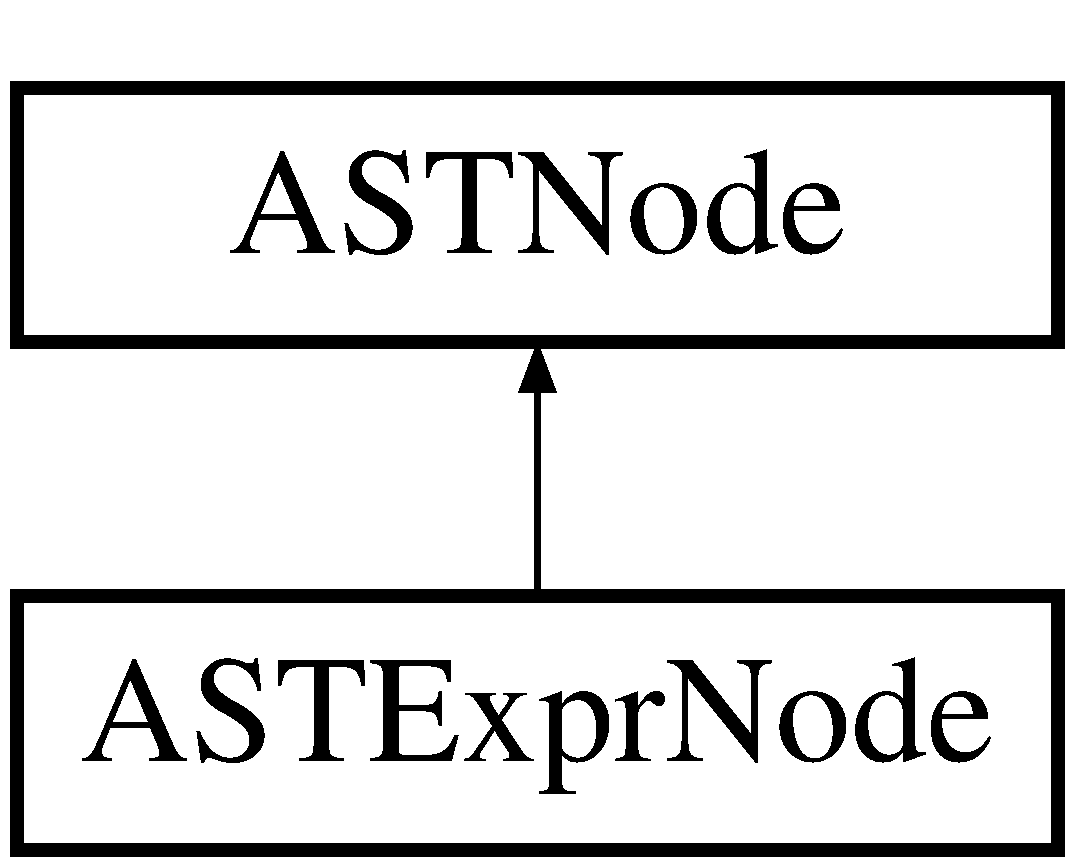
\includegraphics[height=2.000000cm]{class_a_s_t_expr_node}
\end{center}
\end{figure}
\subsection*{Public Member Functions}
\begin{DoxyCompactItemize}
\item 
\hyperlink{class_a_s_t_expr_node_ab239cadd56dc305eba5352a91a8a5499}{A\-S\-T\-Expr\-Node} (\hyperlink{class_a_s_t_node_a4fd016b5f0e44ea6aca3542d27de3859}{Node\-Type}, int)
\item 
\hyperlink{class_a_s_t_expr_node_a8f009ba4853cc2bbcfc05cd4ad026435}{A\-S\-T\-Expr\-Node} (\hyperlink{class_a_s_t_node_a4fd016b5f0e44ea6aca3542d27de3859}{Node\-Type}, \hyperlink{_a_s_t_expr_node_8h_a4f1a4923fbba2992d48ff9e103b110f5}{Expr})
\item 
\hyperlink{class_a_s_t_expr_node_a6ac628dd48fdff2a9fa0a4bcf8519897}{$\sim$\-A\-S\-T\-Expr\-Node} (void)
\item 
bool \hyperlink{class_a_s_t_expr_node_aaf52939daade8e944719282e5d2ab56c}{is\-Matched} (\hyperlink{_a_s_t_expr_node_8h_a4f1a4923fbba2992d48ff9e103b110f5}{Expr})
\item 
virtual \hyperlink{class_a_s_t_node}{A\-S\-T\-Node} $\ast$ \hyperlink{class_a_s_t_expr_node_a3cc0853d56a228c482fe322737e40d84}{add\-Child} (\hyperlink{class_a_s_t_node}{A\-S\-T\-Node} $\ast$c, int child\-Loc)
\end{DoxyCompactItemize}
\subsection*{Additional Inherited Members}


\subsection{Detailed Description}


Definition at line 6 of file A\-S\-T\-Expr\-Node.\-h.



\subsection{Constructor \& Destructor Documentation}
\hypertarget{class_a_s_t_expr_node_ab239cadd56dc305eba5352a91a8a5499}{\index{A\-S\-T\-Expr\-Node@{A\-S\-T\-Expr\-Node}!A\-S\-T\-Expr\-Node@{A\-S\-T\-Expr\-Node}}
\index{A\-S\-T\-Expr\-Node@{A\-S\-T\-Expr\-Node}!ASTExprNode@{A\-S\-T\-Expr\-Node}}
\subsubsection[{A\-S\-T\-Expr\-Node}]{\setlength{\rightskip}{0pt plus 5cm}A\-S\-T\-Expr\-Node\-::\-A\-S\-T\-Expr\-Node (
\begin{DoxyParamCaption}
\item[{{\bf Node\-Type}}]{node\-Type, }
\item[{int}]{value}
\end{DoxyParamCaption}
)}}\label{class_a_s_t_expr_node_ab239cadd56dc305eba5352a91a8a5499}


Definition at line 8 of file A\-S\-T\-Expr\-Node.\-cpp.

\hypertarget{class_a_s_t_expr_node_a8f009ba4853cc2bbcfc05cd4ad026435}{\index{A\-S\-T\-Expr\-Node@{A\-S\-T\-Expr\-Node}!A\-S\-T\-Expr\-Node@{A\-S\-T\-Expr\-Node}}
\index{A\-S\-T\-Expr\-Node@{A\-S\-T\-Expr\-Node}!ASTExprNode@{A\-S\-T\-Expr\-Node}}
\subsubsection[{A\-S\-T\-Expr\-Node}]{\setlength{\rightskip}{0pt plus 5cm}A\-S\-T\-Expr\-Node\-::\-A\-S\-T\-Expr\-Node (
\begin{DoxyParamCaption}
\item[{{\bf Node\-Type}}]{node\-Type, }
\item[{{\bf Expr}}]{value}
\end{DoxyParamCaption}
)}}\label{class_a_s_t_expr_node_a8f009ba4853cc2bbcfc05cd4ad026435}


Definition at line 34 of file A\-S\-T\-Expr\-Node.\-cpp.

\hypertarget{class_a_s_t_expr_node_a6ac628dd48fdff2a9fa0a4bcf8519897}{\index{A\-S\-T\-Expr\-Node@{A\-S\-T\-Expr\-Node}!$\sim$\-A\-S\-T\-Expr\-Node@{$\sim$\-A\-S\-T\-Expr\-Node}}
\index{$\sim$\-A\-S\-T\-Expr\-Node@{$\sim$\-A\-S\-T\-Expr\-Node}!ASTExprNode@{A\-S\-T\-Expr\-Node}}
\subsubsection[{$\sim$\-A\-S\-T\-Expr\-Node}]{\setlength{\rightskip}{0pt plus 5cm}A\-S\-T\-Expr\-Node\-::$\sim$\-A\-S\-T\-Expr\-Node (
\begin{DoxyParamCaption}
\item[{void}]{}
\end{DoxyParamCaption}
)}}\label{class_a_s_t_expr_node_a6ac628dd48fdff2a9fa0a4bcf8519897}


Definition at line 108 of file A\-S\-T\-Expr\-Node.\-cpp.



\subsection{Member Function Documentation}
\hypertarget{class_a_s_t_expr_node_a3cc0853d56a228c482fe322737e40d84}{\index{A\-S\-T\-Expr\-Node@{A\-S\-T\-Expr\-Node}!add\-Child@{add\-Child}}
\index{add\-Child@{add\-Child}!ASTExprNode@{A\-S\-T\-Expr\-Node}}
\subsubsection[{add\-Child}]{\setlength{\rightskip}{0pt plus 5cm}{\bf A\-S\-T\-Node} $\ast$ A\-S\-T\-Expr\-Node\-::add\-Child (
\begin{DoxyParamCaption}
\item[{{\bf A\-S\-T\-Node} $\ast$}]{c, }
\item[{int}]{child\-Loc}
\end{DoxyParamCaption}
)\hspace{0.3cm}{\ttfamily [virtual]}}}\label{class_a_s_t_expr_node_a3cc0853d56a228c482fe322737e40d84}


Definition at line 64 of file A\-S\-T\-Expr\-Node.\-cpp.

\hypertarget{class_a_s_t_expr_node_aaf52939daade8e944719282e5d2ab56c}{\index{A\-S\-T\-Expr\-Node@{A\-S\-T\-Expr\-Node}!is\-Matched@{is\-Matched}}
\index{is\-Matched@{is\-Matched}!ASTExprNode@{A\-S\-T\-Expr\-Node}}
\subsubsection[{is\-Matched}]{\setlength{\rightskip}{0pt plus 5cm}bool A\-S\-T\-Expr\-Node\-::is\-Matched (
\begin{DoxyParamCaption}
\item[{{\bf Expr}}]{expr}
\end{DoxyParamCaption}
)}}\label{class_a_s_t_expr_node_aaf52939daade8e944719282e5d2ab56c}


Definition at line 112 of file A\-S\-T\-Expr\-Node.\-cpp.



The documentation for this class was generated from the following files\-:\begin{DoxyCompactItemize}
\item 
F\-:/3201\-\_\-3202/\-S\-P\-A/\$\-P@/\-S\-P\-A/\-S\-P\-A/\hyperlink{_a_s_t_expr_node_8h}{A\-S\-T\-Expr\-Node.\-h}\item 
F\-:/3201\-\_\-3202/\-S\-P\-A/\$\-P@/\-S\-P\-A/\-S\-P\-A/\hyperlink{_a_s_t_expr_node_8cpp}{A\-S\-T\-Expr\-Node.\-cpp}\end{DoxyCompactItemize}

\hypertarget{class_a_s_t_node}{\section{A\-S\-T\-Node Class Reference}
\label{class_a_s_t_node}\index{A\-S\-T\-Node@{A\-S\-T\-Node}}
}


{\ttfamily \#include $<$A\-S\-T\-Node.\-h$>$}

Inheritance diagram for A\-S\-T\-Node\-:\begin{figure}[H]
\begin{center}
\leavevmode
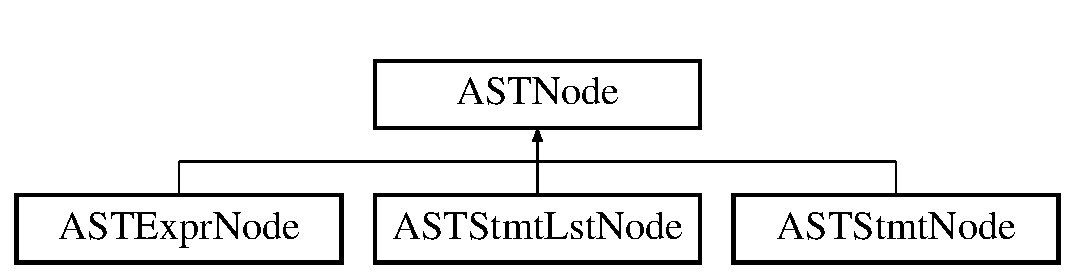
\includegraphics[height=2.000000cm]{class_a_s_t_node}
\end{center}
\end{figure}
\subsection*{Public Types}
\begin{DoxyCompactItemize}
\item 
enum \hyperlink{class_a_s_t_node_a4fd016b5f0e44ea6aca3542d27de3859}{Node\-Type} \{ \\*
\hyperlink{class_a_s_t_node_a4fd016b5f0e44ea6aca3542d27de3859a677c3ce5f7357040776de23f9999fb32}{Program}, 
\hyperlink{class_a_s_t_node_a4fd016b5f0e44ea6aca3542d27de3859a96afa6f10aedf44a6e509b83015d8196}{Procedure}, 
\hyperlink{class_a_s_t_node_a4fd016b5f0e44ea6aca3542d27de3859a3268f5ccc42956fa2011adac0700803d}{Stmt\-Lst}, 
\hyperlink{class_a_s_t_node_a4fd016b5f0e44ea6aca3542d27de3859abc11d3cef1a08db1d7489c8a70c73c75}{Assign}, 
\\*
\hyperlink{class_a_s_t_node_a4fd016b5f0e44ea6aca3542d27de3859a20e38466c592b716e5ac11969753de1c}{Call}, 
\hyperlink{class_a_s_t_node_a4fd016b5f0e44ea6aca3542d27de3859a57ddbd1d98e862fd5deaeec85c5483c4}{While}, 
\hyperlink{class_a_s_t_node_a4fd016b5f0e44ea6aca3542d27de3859a2c6c2af563ff11ef2e968214c790593c}{If}, 
\hyperlink{class_a_s_t_node_a4fd016b5f0e44ea6aca3542d27de3859a4ea10d7791557fbcf1057136cf012e16}{Operator}, 
\\*
\hyperlink{class_a_s_t_node_a4fd016b5f0e44ea6aca3542d27de3859ad1626bafffaf48dc7bd22f2f13f5a50a}{Variable}, 
\hyperlink{class_a_s_t_node_a4fd016b5f0e44ea6aca3542d27de3859a114b1c32de0827e6ee5ff81613b5bb19}{Constant}
 \}
\end{DoxyCompactItemize}
\subsection*{Public Member Functions}
\begin{DoxyCompactItemize}
\item 
\hyperlink{class_a_s_t_node_a1196ed4f19c0b62cdc42fe35946b91d2}{A\-S\-T\-Node} ()
\item 
\hyperlink{class_a_s_t_node_a512c4363de4ceef82b6189e1dbd34ec1}{A\-S\-T\-Node} (\hyperlink{class_a_s_t_node_a4fd016b5f0e44ea6aca3542d27de3859}{Node\-Type})
\item 
\hyperlink{class_a_s_t_node_a97d3345ffb311a0582a8bf1478722a70}{A\-S\-T\-Node} (\hyperlink{class_a_s_t_node_a4fd016b5f0e44ea6aca3542d27de3859}{Node\-Type}, \hyperlink{std_afx_8h_aa07ea1d188c7b45668f1bd82ffd6d87e}{P\-R\-O\-C})
\item 
\hyperlink{class_a_s_t_node_a075d226c6382610b649193f72902faf7}{$\sim$\-A\-S\-T\-Node} (void)
\item 
virtual \hyperlink{class_a_s_t_node}{A\-S\-T\-Node} $\ast$ \hyperlink{class_a_s_t_node_a595fb15c3e37a7a9e443742dca6483ca}{add\-Child} (\hyperlink{class_a_s_t_node}{A\-S\-T\-Node} $\ast$)
\item 
virtual \hyperlink{class_a_s_t_node}{A\-S\-T\-Node} $\ast$ \hyperlink{class_a_s_t_node_a70e8aa10baa353684ae8288f3460a5fc}{set\-Parent} (\hyperlink{class_a_s_t_node}{A\-S\-T\-Node} $\ast$p)
\item 
void \hyperlink{class_a_s_t_node_a940adeca834d8d00d6d9fa70be68bc0f}{set\-Root} (int)
\item 
\hyperlink{class_a_s_t_node_a4fd016b5f0e44ea6aca3542d27de3859}{A\-S\-T\-Node\-::\-Node\-Type} \hyperlink{class_a_s_t_node_afa85380e2e00c7b3166d61ae696b8365}{get\-Type} () const 
\item 
\hyperlink{class_a_s_t_node}{A\-S\-T\-Node} $\ast$ \hyperlink{class_a_s_t_node_a68ef18e60e551c9ba047e3d1809d8620}{get\-Child} (unsigned int) const 
\item 
\hyperlink{class_a_s_t_node}{A\-S\-T\-Node} $\ast$ \hyperlink{class_a_s_t_node_a62e103d706cfbace82cf124bbd080c3e}{get\-Parent} ()
\item 
int \hyperlink{class_a_s_t_node_a899c8bb0314158fc8ca7d5688b89e165}{get\-Value} () const 
\item 
bool \hyperlink{class_a_s_t_node_ae26a0a4a3beebf3ef460ff603cbc3a97}{is\-Has\-Children} ()
\item 
bool \hyperlink{class_a_s_t_node_aba44d4dd6234cab7a2c3f153b65bd97f}{is\-Root} ()
\end{DoxyCompactItemize}
\subsection*{Protected Attributes}
\begin{DoxyCompactItemize}
\item 
int \hyperlink{class_a_s_t_node_a136d1712e8cfdeb4908aceb22abc3de7}{value}
\item 
\hyperlink{class_a_s_t_node}{A\-S\-T\-Node} $\ast$ \hyperlink{class_a_s_t_node_aaa1e479bfeb485d93a4866f9c2daf171}{parent}
\item 
vector$<$ \hyperlink{class_a_s_t_node}{A\-S\-T\-Node} $\ast$ $>$ \hyperlink{class_a_s_t_node_af8f4491cf9294805337542d5873c85b2}{children}
\item 
\hyperlink{class_a_s_t_node_a4fd016b5f0e44ea6aca3542d27de3859}{Node\-Type} \hyperlink{class_a_s_t_node_a15fcdbd8403a1169b06d948a827fde55}{node\-Type}
\end{DoxyCompactItemize}


\subsection{Detailed Description}


Definition at line 5 of file A\-S\-T\-Node.\-h.



\subsection{Member Enumeration Documentation}
\hypertarget{class_a_s_t_node_a4fd016b5f0e44ea6aca3542d27de3859}{\index{A\-S\-T\-Node@{A\-S\-T\-Node}!Node\-Type@{Node\-Type}}
\index{Node\-Type@{Node\-Type}!ASTNode@{A\-S\-T\-Node}}
\subsubsection[{Node\-Type}]{\setlength{\rightskip}{0pt plus 5cm}enum {\bf A\-S\-T\-Node\-::\-Node\-Type}}}\label{class_a_s_t_node_a4fd016b5f0e44ea6aca3542d27de3859}
\begin{Desc}
\item[Enumerator]\par
\begin{description}
\index{Program@{Program}!A\-S\-T\-Node@{A\-S\-T\-Node}}\index{A\-S\-T\-Node@{A\-S\-T\-Node}!Program@{Program}}\item[{\em 
\hypertarget{class_a_s_t_node_a4fd016b5f0e44ea6aca3542d27de3859a677c3ce5f7357040776de23f9999fb32}{Program}\label{class_a_s_t_node_a4fd016b5f0e44ea6aca3542d27de3859a677c3ce5f7357040776de23f9999fb32}
}]\index{Procedure@{Procedure}!A\-S\-T\-Node@{A\-S\-T\-Node}}\index{A\-S\-T\-Node@{A\-S\-T\-Node}!Procedure@{Procedure}}\item[{\em 
\hypertarget{class_a_s_t_node_a4fd016b5f0e44ea6aca3542d27de3859a96afa6f10aedf44a6e509b83015d8196}{Procedure}\label{class_a_s_t_node_a4fd016b5f0e44ea6aca3542d27de3859a96afa6f10aedf44a6e509b83015d8196}
}]\index{Stmt\-Lst@{Stmt\-Lst}!A\-S\-T\-Node@{A\-S\-T\-Node}}\index{A\-S\-T\-Node@{A\-S\-T\-Node}!Stmt\-Lst@{Stmt\-Lst}}\item[{\em 
\hypertarget{class_a_s_t_node_a4fd016b5f0e44ea6aca3542d27de3859a3268f5ccc42956fa2011adac0700803d}{Stmt\-Lst}\label{class_a_s_t_node_a4fd016b5f0e44ea6aca3542d27de3859a3268f5ccc42956fa2011adac0700803d}
}]\index{Assign@{Assign}!A\-S\-T\-Node@{A\-S\-T\-Node}}\index{A\-S\-T\-Node@{A\-S\-T\-Node}!Assign@{Assign}}\item[{\em 
\hypertarget{class_a_s_t_node_a4fd016b5f0e44ea6aca3542d27de3859abc11d3cef1a08db1d7489c8a70c73c75}{Assign}\label{class_a_s_t_node_a4fd016b5f0e44ea6aca3542d27de3859abc11d3cef1a08db1d7489c8a70c73c75}
}]\index{Call@{Call}!A\-S\-T\-Node@{A\-S\-T\-Node}}\index{A\-S\-T\-Node@{A\-S\-T\-Node}!Call@{Call}}\item[{\em 
\hypertarget{class_a_s_t_node_a4fd016b5f0e44ea6aca3542d27de3859a20e38466c592b716e5ac11969753de1c}{Call}\label{class_a_s_t_node_a4fd016b5f0e44ea6aca3542d27de3859a20e38466c592b716e5ac11969753de1c}
}]\index{While@{While}!A\-S\-T\-Node@{A\-S\-T\-Node}}\index{A\-S\-T\-Node@{A\-S\-T\-Node}!While@{While}}\item[{\em 
\hypertarget{class_a_s_t_node_a4fd016b5f0e44ea6aca3542d27de3859a57ddbd1d98e862fd5deaeec85c5483c4}{While}\label{class_a_s_t_node_a4fd016b5f0e44ea6aca3542d27de3859a57ddbd1d98e862fd5deaeec85c5483c4}
}]\index{If@{If}!A\-S\-T\-Node@{A\-S\-T\-Node}}\index{A\-S\-T\-Node@{A\-S\-T\-Node}!If@{If}}\item[{\em 
\hypertarget{class_a_s_t_node_a4fd016b5f0e44ea6aca3542d27de3859a2c6c2af563ff11ef2e968214c790593c}{If}\label{class_a_s_t_node_a4fd016b5f0e44ea6aca3542d27de3859a2c6c2af563ff11ef2e968214c790593c}
}]\index{Operator@{Operator}!A\-S\-T\-Node@{A\-S\-T\-Node}}\index{A\-S\-T\-Node@{A\-S\-T\-Node}!Operator@{Operator}}\item[{\em 
\hypertarget{class_a_s_t_node_a4fd016b5f0e44ea6aca3542d27de3859a4ea10d7791557fbcf1057136cf012e16}{Operator}\label{class_a_s_t_node_a4fd016b5f0e44ea6aca3542d27de3859a4ea10d7791557fbcf1057136cf012e16}
}]\index{Variable@{Variable}!A\-S\-T\-Node@{A\-S\-T\-Node}}\index{A\-S\-T\-Node@{A\-S\-T\-Node}!Variable@{Variable}}\item[{\em 
\hypertarget{class_a_s_t_node_a4fd016b5f0e44ea6aca3542d27de3859ad1626bafffaf48dc7bd22f2f13f5a50a}{Variable}\label{class_a_s_t_node_a4fd016b5f0e44ea6aca3542d27de3859ad1626bafffaf48dc7bd22f2f13f5a50a}
}]\index{Constant@{Constant}!A\-S\-T\-Node@{A\-S\-T\-Node}}\index{A\-S\-T\-Node@{A\-S\-T\-Node}!Constant@{Constant}}\item[{\em 
\hypertarget{class_a_s_t_node_a4fd016b5f0e44ea6aca3542d27de3859a114b1c32de0827e6ee5ff81613b5bb19}{Constant}\label{class_a_s_t_node_a4fd016b5f0e44ea6aca3542d27de3859a114b1c32de0827e6ee5ff81613b5bb19}
}]\end{description}
\end{Desc}


Definition at line 9 of file A\-S\-T\-Node.\-h.



\subsection{Constructor \& Destructor Documentation}
\hypertarget{class_a_s_t_node_a1196ed4f19c0b62cdc42fe35946b91d2}{\index{A\-S\-T\-Node@{A\-S\-T\-Node}!A\-S\-T\-Node@{A\-S\-T\-Node}}
\index{A\-S\-T\-Node@{A\-S\-T\-Node}!ASTNode@{A\-S\-T\-Node}}
\subsubsection[{A\-S\-T\-Node}]{\setlength{\rightskip}{0pt plus 5cm}A\-S\-T\-Node\-::\-A\-S\-T\-Node (
\begin{DoxyParamCaption}
{}
\end{DoxyParamCaption}
)}}\label{class_a_s_t_node_a1196ed4f19c0b62cdc42fe35946b91d2}


Definition at line 5 of file A\-S\-T\-Node.\-cpp.

\hypertarget{class_a_s_t_node_a512c4363de4ceef82b6189e1dbd34ec1}{\index{A\-S\-T\-Node@{A\-S\-T\-Node}!A\-S\-T\-Node@{A\-S\-T\-Node}}
\index{A\-S\-T\-Node@{A\-S\-T\-Node}!ASTNode@{A\-S\-T\-Node}}
\subsubsection[{A\-S\-T\-Node}]{\setlength{\rightskip}{0pt plus 5cm}A\-S\-T\-Node\-::\-A\-S\-T\-Node (
\begin{DoxyParamCaption}
\item[{{\bf Node\-Type}}]{type}
\end{DoxyParamCaption}
)}}\label{class_a_s_t_node_a512c4363de4ceef82b6189e1dbd34ec1}


Definition at line 10 of file A\-S\-T\-Node.\-cpp.

\hypertarget{class_a_s_t_node_a97d3345ffb311a0582a8bf1478722a70}{\index{A\-S\-T\-Node@{A\-S\-T\-Node}!A\-S\-T\-Node@{A\-S\-T\-Node}}
\index{A\-S\-T\-Node@{A\-S\-T\-Node}!ASTNode@{A\-S\-T\-Node}}
\subsubsection[{A\-S\-T\-Node}]{\setlength{\rightskip}{0pt plus 5cm}A\-S\-T\-Node\-::\-A\-S\-T\-Node (
\begin{DoxyParamCaption}
\item[{{\bf Node\-Type}}]{type, }
\item[{{\bf P\-R\-O\-C}}]{p}
\end{DoxyParamCaption}
)}}\label{class_a_s_t_node_a97d3345ffb311a0582a8bf1478722a70}


Definition at line 23 of file A\-S\-T\-Node.\-cpp.

\hypertarget{class_a_s_t_node_a075d226c6382610b649193f72902faf7}{\index{A\-S\-T\-Node@{A\-S\-T\-Node}!$\sim$\-A\-S\-T\-Node@{$\sim$\-A\-S\-T\-Node}}
\index{$\sim$\-A\-S\-T\-Node@{$\sim$\-A\-S\-T\-Node}!ASTNode@{A\-S\-T\-Node}}
\subsubsection[{$\sim$\-A\-S\-T\-Node}]{\setlength{\rightskip}{0pt plus 5cm}A\-S\-T\-Node\-::$\sim$\-A\-S\-T\-Node (
\begin{DoxyParamCaption}
\item[{void}]{}
\end{DoxyParamCaption}
)}}\label{class_a_s_t_node_a075d226c6382610b649193f72902faf7}


Definition at line 131 of file A\-S\-T\-Node.\-cpp.



\subsection{Member Function Documentation}
\hypertarget{class_a_s_t_node_a595fb15c3e37a7a9e443742dca6483ca}{\index{A\-S\-T\-Node@{A\-S\-T\-Node}!add\-Child@{add\-Child}}
\index{add\-Child@{add\-Child}!ASTNode@{A\-S\-T\-Node}}
\subsubsection[{add\-Child}]{\setlength{\rightskip}{0pt plus 5cm}{\bf A\-S\-T\-Node} $\ast$ A\-S\-T\-Node\-::add\-Child (
\begin{DoxyParamCaption}
\item[{{\bf A\-S\-T\-Node} $\ast$}]{c}
\end{DoxyParamCaption}
)\hspace{0.3cm}{\ttfamily [virtual]}}}\label{class_a_s_t_node_a595fb15c3e37a7a9e443742dca6483ca}


Reimplemented in \hyperlink{class_a_s_t_stmt_node_a0396498d6bbccecd8a71a4251d237380}{A\-S\-T\-Stmt\-Node}, and \hyperlink{class_a_s_t_stmt_lst_node_a5424fe2ed759c533a1c26e6172dae45f}{A\-S\-T\-Stmt\-Lst\-Node}.



Definition at line 55 of file A\-S\-T\-Node.\-cpp.

\hypertarget{class_a_s_t_node_a68ef18e60e551c9ba047e3d1809d8620}{\index{A\-S\-T\-Node@{A\-S\-T\-Node}!get\-Child@{get\-Child}}
\index{get\-Child@{get\-Child}!ASTNode@{A\-S\-T\-Node}}
\subsubsection[{get\-Child}]{\setlength{\rightskip}{0pt plus 5cm}{\bf A\-S\-T\-Node} $\ast$ A\-S\-T\-Node\-::get\-Child (
\begin{DoxyParamCaption}
\item[{unsigned int}]{i}
\end{DoxyParamCaption}
) const}}\label{class_a_s_t_node_a68ef18e60e551c9ba047e3d1809d8620}


Definition at line 117 of file A\-S\-T\-Node.\-cpp.

\hypertarget{class_a_s_t_node_a62e103d706cfbace82cf124bbd080c3e}{\index{A\-S\-T\-Node@{A\-S\-T\-Node}!get\-Parent@{get\-Parent}}
\index{get\-Parent@{get\-Parent}!ASTNode@{A\-S\-T\-Node}}
\subsubsection[{get\-Parent}]{\setlength{\rightskip}{0pt plus 5cm}{\bf A\-S\-T\-Node} $\ast$ A\-S\-T\-Node\-::get\-Parent (
\begin{DoxyParamCaption}
{}
\end{DoxyParamCaption}
)}}\label{class_a_s_t_node_a62e103d706cfbace82cf124bbd080c3e}


Definition at line 126 of file A\-S\-T\-Node.\-cpp.

\hypertarget{class_a_s_t_node_afa85380e2e00c7b3166d61ae696b8365}{\index{A\-S\-T\-Node@{A\-S\-T\-Node}!get\-Type@{get\-Type}}
\index{get\-Type@{get\-Type}!ASTNode@{A\-S\-T\-Node}}
\subsubsection[{get\-Type}]{\setlength{\rightskip}{0pt plus 5cm}{\bf A\-S\-T\-Node\-::\-Node\-Type} A\-S\-T\-Node\-::get\-Type (
\begin{DoxyParamCaption}
{}
\end{DoxyParamCaption}
) const}}\label{class_a_s_t_node_afa85380e2e00c7b3166d61ae696b8365}


Definition at line 112 of file A\-S\-T\-Node.\-cpp.

\hypertarget{class_a_s_t_node_a899c8bb0314158fc8ca7d5688b89e165}{\index{A\-S\-T\-Node@{A\-S\-T\-Node}!get\-Value@{get\-Value}}
\index{get\-Value@{get\-Value}!ASTNode@{A\-S\-T\-Node}}
\subsubsection[{get\-Value}]{\setlength{\rightskip}{0pt plus 5cm}int A\-S\-T\-Node\-::get\-Value (
\begin{DoxyParamCaption}
{}
\end{DoxyParamCaption}
) const}}\label{class_a_s_t_node_a899c8bb0314158fc8ca7d5688b89e165}


Definition at line 37 of file A\-S\-T\-Node.\-cpp.

\hypertarget{class_a_s_t_node_ae26a0a4a3beebf3ef460ff603cbc3a97}{\index{A\-S\-T\-Node@{A\-S\-T\-Node}!is\-Has\-Children@{is\-Has\-Children}}
\index{is\-Has\-Children@{is\-Has\-Children}!ASTNode@{A\-S\-T\-Node}}
\subsubsection[{is\-Has\-Children}]{\setlength{\rightskip}{0pt plus 5cm}bool A\-S\-T\-Node\-::is\-Has\-Children (
\begin{DoxyParamCaption}
{}
\end{DoxyParamCaption}
)}}\label{class_a_s_t_node_ae26a0a4a3beebf3ef460ff603cbc3a97}


Definition at line 106 of file A\-S\-T\-Node.\-cpp.

\hypertarget{class_a_s_t_node_aba44d4dd6234cab7a2c3f153b65bd97f}{\index{A\-S\-T\-Node@{A\-S\-T\-Node}!is\-Root@{is\-Root}}
\index{is\-Root@{is\-Root}!ASTNode@{A\-S\-T\-Node}}
\subsubsection[{is\-Root}]{\setlength{\rightskip}{0pt plus 5cm}bool A\-S\-T\-Node\-::is\-Root (
\begin{DoxyParamCaption}
{}
\end{DoxyParamCaption}
)}}\label{class_a_s_t_node_aba44d4dd6234cab7a2c3f153b65bd97f}


Definition at line 101 of file A\-S\-T\-Node.\-cpp.

\hypertarget{class_a_s_t_node_a70e8aa10baa353684ae8288f3460a5fc}{\index{A\-S\-T\-Node@{A\-S\-T\-Node}!set\-Parent@{set\-Parent}}
\index{set\-Parent@{set\-Parent}!ASTNode@{A\-S\-T\-Node}}
\subsubsection[{set\-Parent}]{\setlength{\rightskip}{0pt plus 5cm}{\bf A\-S\-T\-Node} $\ast$ A\-S\-T\-Node\-::set\-Parent (
\begin{DoxyParamCaption}
\item[{{\bf A\-S\-T\-Node} $\ast$}]{p}
\end{DoxyParamCaption}
)\hspace{0.3cm}{\ttfamily [virtual]}}}\label{class_a_s_t_node_a70e8aa10baa353684ae8288f3460a5fc}


Definition at line 43 of file A\-S\-T\-Node.\-cpp.

\hypertarget{class_a_s_t_node_a940adeca834d8d00d6d9fa70be68bc0f}{\index{A\-S\-T\-Node@{A\-S\-T\-Node}!set\-Root@{set\-Root}}
\index{set\-Root@{set\-Root}!ASTNode@{A\-S\-T\-Node}}
\subsubsection[{set\-Root}]{\setlength{\rightskip}{0pt plus 5cm}void A\-S\-T\-Node\-::set\-Root (
\begin{DoxyParamCaption}
\item[{int}]{P\-R\-O\-C\-Index}
\end{DoxyParamCaption}
)}}\label{class_a_s_t_node_a940adeca834d8d00d6d9fa70be68bc0f}


Definition at line 91 of file A\-S\-T\-Node.\-cpp.



\subsection{Member Data Documentation}
\hypertarget{class_a_s_t_node_af8f4491cf9294805337542d5873c85b2}{\index{A\-S\-T\-Node@{A\-S\-T\-Node}!children@{children}}
\index{children@{children}!ASTNode@{A\-S\-T\-Node}}
\subsubsection[{children}]{\setlength{\rightskip}{0pt plus 5cm}vector$<${\bf A\-S\-T\-Node}$\ast$$>$ A\-S\-T\-Node\-::children\hspace{0.3cm}{\ttfamily [protected]}}}\label{class_a_s_t_node_af8f4491cf9294805337542d5873c85b2}


Definition at line 56 of file A\-S\-T\-Node.\-h.

\hypertarget{class_a_s_t_node_a15fcdbd8403a1169b06d948a827fde55}{\index{A\-S\-T\-Node@{A\-S\-T\-Node}!node\-Type@{node\-Type}}
\index{node\-Type@{node\-Type}!ASTNode@{A\-S\-T\-Node}}
\subsubsection[{node\-Type}]{\setlength{\rightskip}{0pt plus 5cm}{\bf Node\-Type} A\-S\-T\-Node\-::node\-Type\hspace{0.3cm}{\ttfamily [protected]}}}\label{class_a_s_t_node_a15fcdbd8403a1169b06d948a827fde55}


Definition at line 57 of file A\-S\-T\-Node.\-h.

\hypertarget{class_a_s_t_node_aaa1e479bfeb485d93a4866f9c2daf171}{\index{A\-S\-T\-Node@{A\-S\-T\-Node}!parent@{parent}}
\index{parent@{parent}!ASTNode@{A\-S\-T\-Node}}
\subsubsection[{parent}]{\setlength{\rightskip}{0pt plus 5cm}{\bf A\-S\-T\-Node}$\ast$ A\-S\-T\-Node\-::parent\hspace{0.3cm}{\ttfamily [protected]}}}\label{class_a_s_t_node_aaa1e479bfeb485d93a4866f9c2daf171}


Definition at line 55 of file A\-S\-T\-Node.\-h.

\hypertarget{class_a_s_t_node_a136d1712e8cfdeb4908aceb22abc3de7}{\index{A\-S\-T\-Node@{A\-S\-T\-Node}!value@{value}}
\index{value@{value}!ASTNode@{A\-S\-T\-Node}}
\subsubsection[{value}]{\setlength{\rightskip}{0pt plus 5cm}int A\-S\-T\-Node\-::value\hspace{0.3cm}{\ttfamily [protected]}}}\label{class_a_s_t_node_a136d1712e8cfdeb4908aceb22abc3de7}


Definition at line 54 of file A\-S\-T\-Node.\-h.



The documentation for this class was generated from the following files\-:\begin{DoxyCompactItemize}
\item 
F\-:/3201\-\_\-3202/\-S\-P\-A/\$\-P@/\-S\-P\-A/\-S\-P\-A/\hyperlink{_a_s_t_node_8h}{A\-S\-T\-Node.\-h}\item 
F\-:/3201\-\_\-3202/\-S\-P\-A/\$\-P@/\-S\-P\-A/\-S\-P\-A/\hyperlink{_a_s_t_node_8cpp}{A\-S\-T\-Node.\-cpp}\end{DoxyCompactItemize}

\hypertarget{class_a_s_t_stmt_lst_node}{\section{A\-S\-T\-Stmt\-Lst\-Node Class Reference}
\label{class_a_s_t_stmt_lst_node}\index{A\-S\-T\-Stmt\-Lst\-Node@{A\-S\-T\-Stmt\-Lst\-Node}}
}


{\ttfamily \#include $<$A\-S\-T\-Stmt\-Lst\-Node.\-h$>$}

Inheritance diagram for A\-S\-T\-Stmt\-Lst\-Node\-:\begin{figure}[H]
\begin{center}
\leavevmode
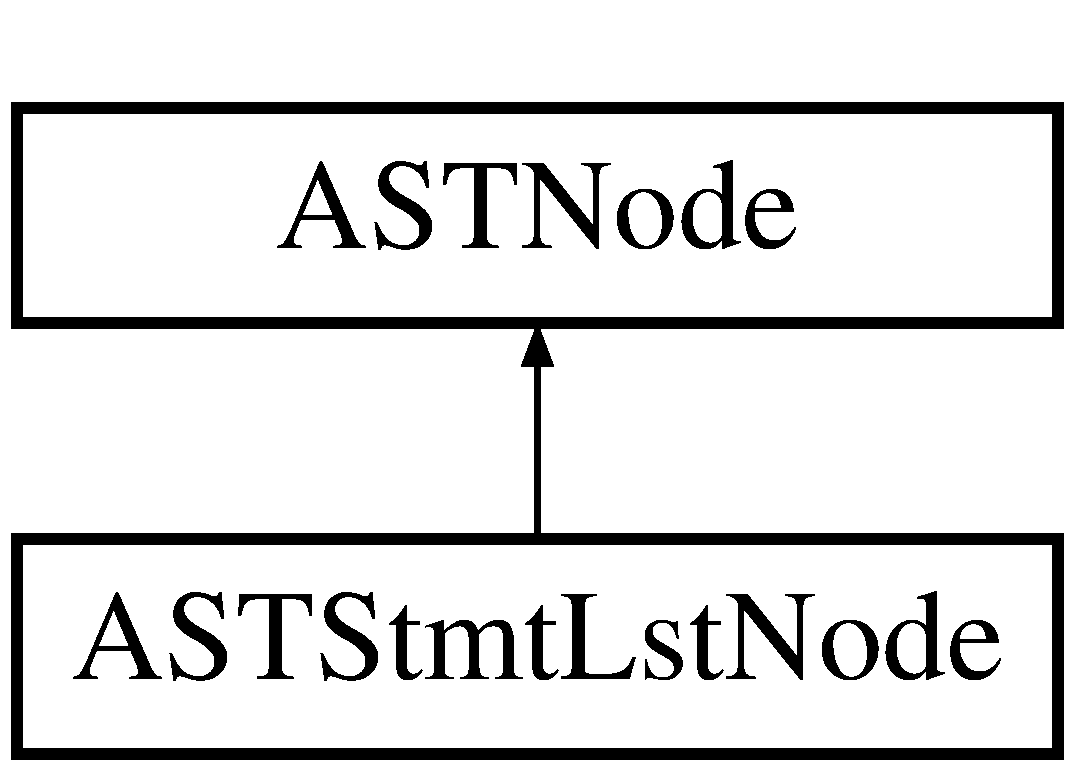
\includegraphics[height=2.000000cm]{class_a_s_t_stmt_lst_node}
\end{center}
\end{figure}
\subsection*{Public Member Functions}
\begin{DoxyCompactItemize}
\item 
\hyperlink{class_a_s_t_stmt_lst_node_a12c10755015930be83b22f9edd75f610}{A\-S\-T\-Stmt\-Lst\-Node} ()
\item 
\hyperlink{class_a_s_t_stmt_lst_node_a9d5ab5a42f1b92642e14d15a03a2e4e3}{$\sim$\-A\-S\-T\-Stmt\-Lst\-Node} (void)
\item 
int \hyperlink{class_a_s_t_stmt_lst_node_a49f21aa9b4b7836943762aee8f5ffae0}{get\-Size} ()
\item 
virtual \hyperlink{class_a_s_t_node}{A\-S\-T\-Node} $\ast$ \hyperlink{class_a_s_t_stmt_lst_node_a5424fe2ed759c533a1c26e6172dae45f}{add\-Child} (\hyperlink{class_a_s_t_node}{A\-S\-T\-Node} $\ast$)
\end{DoxyCompactItemize}
\subsection*{Additional Inherited Members}


\subsection{Detailed Description}


Definition at line 7 of file A\-S\-T\-Stmt\-Lst\-Node.\-h.



\subsection{Constructor \& Destructor Documentation}
\hypertarget{class_a_s_t_stmt_lst_node_a12c10755015930be83b22f9edd75f610}{\index{A\-S\-T\-Stmt\-Lst\-Node@{A\-S\-T\-Stmt\-Lst\-Node}!A\-S\-T\-Stmt\-Lst\-Node@{A\-S\-T\-Stmt\-Lst\-Node}}
\index{A\-S\-T\-Stmt\-Lst\-Node@{A\-S\-T\-Stmt\-Lst\-Node}!ASTStmtLstNode@{A\-S\-T\-Stmt\-Lst\-Node}}
\subsubsection[{A\-S\-T\-Stmt\-Lst\-Node}]{\setlength{\rightskip}{0pt plus 5cm}A\-S\-T\-Stmt\-Lst\-Node\-::\-A\-S\-T\-Stmt\-Lst\-Node (
\begin{DoxyParamCaption}
{}
\end{DoxyParamCaption}
)}}\label{class_a_s_t_stmt_lst_node_a12c10755015930be83b22f9edd75f610}


Definition at line 5 of file A\-S\-T\-Stmt\-Lst\-Node.\-cpp.

\hypertarget{class_a_s_t_stmt_lst_node_a9d5ab5a42f1b92642e14d15a03a2e4e3}{\index{A\-S\-T\-Stmt\-Lst\-Node@{A\-S\-T\-Stmt\-Lst\-Node}!$\sim$\-A\-S\-T\-Stmt\-Lst\-Node@{$\sim$\-A\-S\-T\-Stmt\-Lst\-Node}}
\index{$\sim$\-A\-S\-T\-Stmt\-Lst\-Node@{$\sim$\-A\-S\-T\-Stmt\-Lst\-Node}!ASTStmtLstNode@{A\-S\-T\-Stmt\-Lst\-Node}}
\subsubsection[{$\sim$\-A\-S\-T\-Stmt\-Lst\-Node}]{\setlength{\rightskip}{0pt plus 5cm}A\-S\-T\-Stmt\-Lst\-Node\-::$\sim$\-A\-S\-T\-Stmt\-Lst\-Node (
\begin{DoxyParamCaption}
\item[{void}]{}
\end{DoxyParamCaption}
)}}\label{class_a_s_t_stmt_lst_node_a9d5ab5a42f1b92642e14d15a03a2e4e3}


Definition at line 11 of file A\-S\-T\-Stmt\-Lst\-Node.\-cpp.



\subsection{Member Function Documentation}
\hypertarget{class_a_s_t_stmt_lst_node_a5424fe2ed759c533a1c26e6172dae45f}{\index{A\-S\-T\-Stmt\-Lst\-Node@{A\-S\-T\-Stmt\-Lst\-Node}!add\-Child@{add\-Child}}
\index{add\-Child@{add\-Child}!ASTStmtLstNode@{A\-S\-T\-Stmt\-Lst\-Node}}
\subsubsection[{add\-Child}]{\setlength{\rightskip}{0pt plus 5cm}{\bf A\-S\-T\-Node} $\ast$ A\-S\-T\-Stmt\-Lst\-Node\-::add\-Child (
\begin{DoxyParamCaption}
\item[{{\bf A\-S\-T\-Node} $\ast$}]{node}
\end{DoxyParamCaption}
)\hspace{0.3cm}{\ttfamily [virtual]}}}\label{class_a_s_t_stmt_lst_node_a5424fe2ed759c533a1c26e6172dae45f}


Reimplemented from \hyperlink{class_a_s_t_node_a595fb15c3e37a7a9e443742dca6483ca}{A\-S\-T\-Node}.



Definition at line 20 of file A\-S\-T\-Stmt\-Lst\-Node.\-cpp.

\hypertarget{class_a_s_t_stmt_lst_node_a49f21aa9b4b7836943762aee8f5ffae0}{\index{A\-S\-T\-Stmt\-Lst\-Node@{A\-S\-T\-Stmt\-Lst\-Node}!get\-Size@{get\-Size}}
\index{get\-Size@{get\-Size}!ASTStmtLstNode@{A\-S\-T\-Stmt\-Lst\-Node}}
\subsubsection[{get\-Size}]{\setlength{\rightskip}{0pt plus 5cm}int A\-S\-T\-Stmt\-Lst\-Node\-::get\-Size (
\begin{DoxyParamCaption}
{}
\end{DoxyParamCaption}
)}}\label{class_a_s_t_stmt_lst_node_a49f21aa9b4b7836943762aee8f5ffae0}


Definition at line 15 of file A\-S\-T\-Stmt\-Lst\-Node.\-cpp.



The documentation for this class was generated from the following files\-:\begin{DoxyCompactItemize}
\item 
F\-:/3201\-\_\-3202/\-S\-P\-A/\$\-P@/\-S\-P\-A/\-S\-P\-A/\hyperlink{_a_s_t_stmt_lst_node_8h}{A\-S\-T\-Stmt\-Lst\-Node.\-h}\item 
F\-:/3201\-\_\-3202/\-S\-P\-A/\$\-P@/\-S\-P\-A/\-S\-P\-A/\hyperlink{_a_s_t_stmt_lst_node_8cpp}{A\-S\-T\-Stmt\-Lst\-Node.\-cpp}\end{DoxyCompactItemize}

\hypertarget{class_a_s_t_stmt_node}{\section{A\-S\-T\-Stmt\-Node Class Reference}
\label{class_a_s_t_stmt_node}\index{A\-S\-T\-Stmt\-Node@{A\-S\-T\-Stmt\-Node}}
}


{\ttfamily \#include $<$A\-S\-T\-Stmt\-Node.\-h$>$}

Inheritance diagram for A\-S\-T\-Stmt\-Node\-:\begin{figure}[H]
\begin{center}
\leavevmode
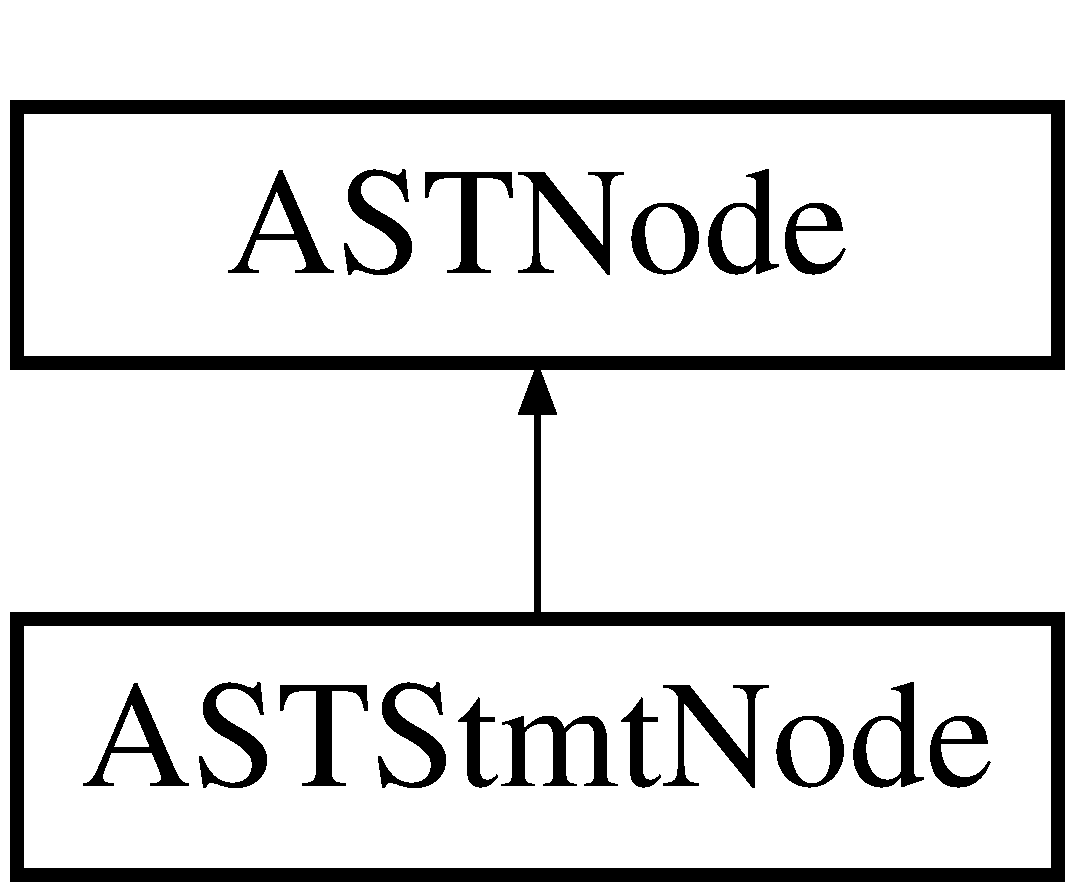
\includegraphics[height=2.000000cm]{class_a_s_t_stmt_node}
\end{center}
\end{figure}
\subsection*{Public Member Functions}
\begin{DoxyCompactItemize}
\item 
\hyperlink{class_a_s_t_stmt_node_abf3ac4ab701786816ee76defcdb3c328}{A\-S\-T\-Stmt\-Node} (int stmt\-No, \hyperlink{class_a_s_t_node_a4fd016b5f0e44ea6aca3542d27de3859}{Node\-Type} \hyperlink{class_a_s_t_node_a15fcdbd8403a1169b06d948a827fde55}{node\-Type}, \hyperlink{_a_s_t_stmt_node_8h_a4a0e50e01fef3e431767a928c2631cab}{Index} \hyperlink{class_a_s_t_node_a136d1712e8cfdeb4908aceb22abc3de7}{value})
\item 
\hyperlink{class_a_s_t_stmt_node_ac80a1656c17e5e55dff7285fd37dc313}{$\sim$\-A\-S\-T\-Stmt\-Node} ()
\item 
int \hyperlink{class_a_s_t_stmt_node_a7ccabe8c03f4ba0eb31ac4850725c4e2}{get\-Stmt\-Number} ()
\item 
virtual \hyperlink{class_a_s_t_node}{A\-S\-T\-Node} $\ast$ \hyperlink{class_a_s_t_stmt_node_a0396498d6bbccecd8a71a4251d237380}{add\-Child} (\hyperlink{class_a_s_t_node}{A\-S\-T\-Node} $\ast$c)
\item 
virtual \hyperlink{class_a_s_t_node}{A\-S\-T\-Node} $\ast$ \hyperlink{class_a_s_t_stmt_node_aa265b32dab6bb7fcb8b7f1e8a9687f9a}{add\-Child} (\hyperlink{class_a_s_t_node}{A\-S\-T\-Node} $\ast$c, int child\-Loc)
\end{DoxyCompactItemize}
\subsection*{Additional Inherited Members}


\subsection{Detailed Description}


Definition at line 7 of file A\-S\-T\-Stmt\-Node.\-h.



\subsection{Constructor \& Destructor Documentation}
\hypertarget{class_a_s_t_stmt_node_abf3ac4ab701786816ee76defcdb3c328}{\index{A\-S\-T\-Stmt\-Node@{A\-S\-T\-Stmt\-Node}!A\-S\-T\-Stmt\-Node@{A\-S\-T\-Stmt\-Node}}
\index{A\-S\-T\-Stmt\-Node@{A\-S\-T\-Stmt\-Node}!ASTStmtNode@{A\-S\-T\-Stmt\-Node}}
\subsubsection[{A\-S\-T\-Stmt\-Node}]{\setlength{\rightskip}{0pt plus 5cm}A\-S\-T\-Stmt\-Node\-::\-A\-S\-T\-Stmt\-Node (
\begin{DoxyParamCaption}
\item[{int}]{stmt\-No, }
\item[{{\bf Node\-Type}}]{node\-Type, }
\item[{{\bf Index}}]{value}
\end{DoxyParamCaption}
)}}\label{class_a_s_t_stmt_node_abf3ac4ab701786816ee76defcdb3c328}


Definition at line 9 of file A\-S\-T\-Stmt\-Node.\-cpp.

\hypertarget{class_a_s_t_stmt_node_ac80a1656c17e5e55dff7285fd37dc313}{\index{A\-S\-T\-Stmt\-Node@{A\-S\-T\-Stmt\-Node}!$\sim$\-A\-S\-T\-Stmt\-Node@{$\sim$\-A\-S\-T\-Stmt\-Node}}
\index{$\sim$\-A\-S\-T\-Stmt\-Node@{$\sim$\-A\-S\-T\-Stmt\-Node}!ASTStmtNode@{A\-S\-T\-Stmt\-Node}}
\subsubsection[{$\sim$\-A\-S\-T\-Stmt\-Node}]{\setlength{\rightskip}{0pt plus 5cm}A\-S\-T\-Stmt\-Node\-::$\sim$\-A\-S\-T\-Stmt\-Node (
\begin{DoxyParamCaption}
{}
\end{DoxyParamCaption}
)}}\label{class_a_s_t_stmt_node_ac80a1656c17e5e55dff7285fd37dc313}


Definition at line 150 of file A\-S\-T\-Stmt\-Node.\-cpp.



\subsection{Member Function Documentation}
\hypertarget{class_a_s_t_stmt_node_a0396498d6bbccecd8a71a4251d237380}{\index{A\-S\-T\-Stmt\-Node@{A\-S\-T\-Stmt\-Node}!add\-Child@{add\-Child}}
\index{add\-Child@{add\-Child}!ASTStmtNode@{A\-S\-T\-Stmt\-Node}}
\subsubsection[{add\-Child}]{\setlength{\rightskip}{0pt plus 5cm}{\bf A\-S\-T\-Node} $\ast$ A\-S\-T\-Stmt\-Node\-::add\-Child (
\begin{DoxyParamCaption}
\item[{{\bf A\-S\-T\-Node} $\ast$}]{c}
\end{DoxyParamCaption}
)\hspace{0.3cm}{\ttfamily [virtual]}}}\label{class_a_s_t_stmt_node_a0396498d6bbccecd8a71a4251d237380}


Reimplemented from \hyperlink{class_a_s_t_node_a595fb15c3e37a7a9e443742dca6483ca}{A\-S\-T\-Node}.



Definition at line 25 of file A\-S\-T\-Stmt\-Node.\-cpp.

\hypertarget{class_a_s_t_stmt_node_aa265b32dab6bb7fcb8b7f1e8a9687f9a}{\index{A\-S\-T\-Stmt\-Node@{A\-S\-T\-Stmt\-Node}!add\-Child@{add\-Child}}
\index{add\-Child@{add\-Child}!ASTStmtNode@{A\-S\-T\-Stmt\-Node}}
\subsubsection[{add\-Child}]{\setlength{\rightskip}{0pt plus 5cm}{\bf A\-S\-T\-Node} $\ast$ A\-S\-T\-Stmt\-Node\-::add\-Child (
\begin{DoxyParamCaption}
\item[{{\bf A\-S\-T\-Node} $\ast$}]{c, }
\item[{int}]{child\-Loc}
\end{DoxyParamCaption}
)\hspace{0.3cm}{\ttfamily [virtual]}}}\label{class_a_s_t_stmt_node_aa265b32dab6bb7fcb8b7f1e8a9687f9a}


Definition at line 54 of file A\-S\-T\-Stmt\-Node.\-cpp.

\hypertarget{class_a_s_t_stmt_node_a7ccabe8c03f4ba0eb31ac4850725c4e2}{\index{A\-S\-T\-Stmt\-Node@{A\-S\-T\-Stmt\-Node}!get\-Stmt\-Number@{get\-Stmt\-Number}}
\index{get\-Stmt\-Number@{get\-Stmt\-Number}!ASTStmtNode@{A\-S\-T\-Stmt\-Node}}
\subsubsection[{get\-Stmt\-Number}]{\setlength{\rightskip}{0pt plus 5cm}int A\-S\-T\-Stmt\-Node\-::get\-Stmt\-Number (
\begin{DoxyParamCaption}
{}
\end{DoxyParamCaption}
)}}\label{class_a_s_t_stmt_node_a7ccabe8c03f4ba0eb31ac4850725c4e2}


Definition at line 154 of file A\-S\-T\-Stmt\-Node.\-cpp.



The documentation for this class was generated from the following files\-:\begin{DoxyCompactItemize}
\item 
F\-:/3201\-\_\-3202/\-S\-P\-A/\$\-P@/\-S\-P\-A/\-S\-P\-A/\hyperlink{_a_s_t_stmt_node_8h}{A\-S\-T\-Stmt\-Node.\-h}\item 
F\-:/3201\-\_\-3202/\-S\-P\-A/\$\-P@/\-S\-P\-A/\-S\-P\-A/\hyperlink{_a_s_t_stmt_node_8cpp}{A\-S\-T\-Stmt\-Node.\-cpp}\end{DoxyCompactItemize}

\hypertarget{class_calls_table}{\section{Calls\-Table Class Reference}
\label{class_calls_table}\index{Calls\-Table@{Calls\-Table}}
}


{\ttfamily \#include $<$Calls\-Table.\-h$>$}

\subsection*{Public Member Functions}
\begin{DoxyCompactItemize}
\item 
\hyperlink{class_calls_table_a852d1327bef61851b3896264b682a4aa}{Calls\-Table} ()
\item 
void \hyperlink{class_calls_table_a8a0b0e665281f2c0d23f255c03282a66}{insert\-Calls} (\hyperlink{std_afx_8h_aa07ea1d188c7b45668f1bd82ffd6d87e}{P\-R\-O\-C}, \hyperlink{std_afx_8h_aa07ea1d188c7b45668f1bd82ffd6d87e}{P\-R\-O\-C})
\item 
vector$<$ \hyperlink{std_afx_8h_aa07ea1d188c7b45668f1bd82ffd6d87e}{P\-R\-O\-C} $>$ \hyperlink{class_calls_table_af50654db975ad7d3b9fa74f8547998eb}{get\-Called\-By} (\hyperlink{std_afx_8h_aa07ea1d188c7b45668f1bd82ffd6d87e}{P\-R\-O\-C})
\item 
vector$<$ \hyperlink{std_afx_8h_aa07ea1d188c7b45668f1bd82ffd6d87e}{P\-R\-O\-C} $>$ \hyperlink{class_calls_table_ade7109a5b16d953b66c49ddeef36eff1}{get\-Called\-From} (\hyperlink{std_afx_8h_aa07ea1d188c7b45668f1bd82ffd6d87e}{P\-R\-O\-C})
\item 
vector$<$ \hyperlink{std_afx_8h_aa07ea1d188c7b45668f1bd82ffd6d87e}{P\-R\-O\-C} $>$ \hyperlink{class_calls_table_a71e96fb0576531152756c529c0bb666f}{get\-Called\-By\-Star} (\hyperlink{std_afx_8h_aa07ea1d188c7b45668f1bd82ffd6d87e}{P\-R\-O\-C})
\item 
vector$<$ \hyperlink{std_afx_8h_aa07ea1d188c7b45668f1bd82ffd6d87e}{P\-R\-O\-C} $>$ \hyperlink{class_calls_table_a3f984929213fdd181d904a9bcd8b99c2}{get\-Called\-From\-Star} (\hyperlink{std_afx_8h_aa07ea1d188c7b45668f1bd82ffd6d87e}{P\-R\-O\-C})
\item 
bool \hyperlink{class_calls_table_a7533cb25ac6b5cfa990a4ab66caa7d84}{is\-Called} (\hyperlink{std_afx_8h_aa07ea1d188c7b45668f1bd82ffd6d87e}{P\-R\-O\-C}, \hyperlink{std_afx_8h_aa07ea1d188c7b45668f1bd82ffd6d87e}{P\-R\-O\-C})
\item 
bool \hyperlink{class_calls_table_a8355c71d51e270130651f17007d3b6a6}{is\-Called\-Star} (\hyperlink{std_afx_8h_aa07ea1d188c7b45668f1bd82ffd6d87e}{P\-R\-O\-C}, \hyperlink{std_afx_8h_aa07ea1d188c7b45668f1bd82ffd6d87e}{P\-R\-O\-C})
\item 
bool \hyperlink{class_calls_table_a5d6f530110e6983be8cef4b6d12b9e78}{is\-Empty} ()
\item 
void \hyperlink{class_calls_table_a978f84e07ad7bafb1737c6a290c8527a}{insert\-Stmt\-Call} (\hyperlink{std_afx_8h_a4a876b28ac3f59cecb39c2d2d76e4e7a}{S\-T\-M\-T}, \hyperlink{std_afx_8h_aa07ea1d188c7b45668f1bd82ffd6d87e}{P\-R\-O\-C})
\item 
vector$<$ \hyperlink{std_afx_8h_a4a876b28ac3f59cecb39c2d2d76e4e7a}{S\-T\-M\-T} $>$ \hyperlink{class_calls_table_ad03ad8e545d3d1225d6388c97ab0d268}{get\-Stmt\-Call} (\hyperlink{std_afx_8h_aa07ea1d188c7b45668f1bd82ffd6d87e}{P\-R\-O\-C})
\item 
void \hyperlink{class_calls_table_a21decabd3099cd7adb4ebfcdbb6bad8d}{optimize\-Calls\-Table} ()
\item 
int \hyperlink{class_calls_table_affa05af1a77dab6c79e2b43824898010}{get\-Calls\-Size} ()
\item 
int \hyperlink{class_calls_table_a9adfb829fa0361df34eadb011f80406e}{get\-Calls\-Star\-Size} ()
\item 
void \hyperlink{class_calls_table_ae9c18d5f905d063cf912ebb2c1ce4cbd}{display\-Calls\-Tables} ()
\end{DoxyCompactItemize}


\subsection{Detailed Description}


Definition at line 4 of file Calls\-Table.\-h.



\subsection{Constructor \& Destructor Documentation}
\hypertarget{class_calls_table_a852d1327bef61851b3896264b682a4aa}{\index{Calls\-Table@{Calls\-Table}!Calls\-Table@{Calls\-Table}}
\index{Calls\-Table@{Calls\-Table}!CallsTable@{Calls\-Table}}
\subsubsection[{Calls\-Table}]{\setlength{\rightskip}{0pt plus 5cm}Calls\-Table\-::\-Calls\-Table (
\begin{DoxyParamCaption}
{}
\end{DoxyParamCaption}
)}}\label{class_calls_table_a852d1327bef61851b3896264b682a4aa}
This method will be used as a constructor to create \hyperlink{class_calls_table}{Calls\-Table} 

Definition at line 8 of file Calls\-Table.\-cpp.



\subsection{Member Function Documentation}
\hypertarget{class_calls_table_ae9c18d5f905d063cf912ebb2c1ce4cbd}{\index{Calls\-Table@{Calls\-Table}!display\-Calls\-Tables@{display\-Calls\-Tables}}
\index{display\-Calls\-Tables@{display\-Calls\-Tables}!CallsTable@{Calls\-Table}}
\subsubsection[{display\-Calls\-Tables}]{\setlength{\rightskip}{0pt plus 5cm}void Calls\-Table\-::display\-Calls\-Tables (
\begin{DoxyParamCaption}
{}
\end{DoxyParamCaption}
)}}\label{class_calls_table_ae9c18d5f905d063cf912ebb2c1ce4cbd}
This method will be used for testing purposes for viewing the content of the Call table 

Definition at line 229 of file Calls\-Table.\-cpp.

\hypertarget{class_calls_table_af50654db975ad7d3b9fa74f8547998eb}{\index{Calls\-Table@{Calls\-Table}!get\-Called\-By@{get\-Called\-By}}
\index{get\-Called\-By@{get\-Called\-By}!CallsTable@{Calls\-Table}}
\subsubsection[{get\-Called\-By}]{\setlength{\rightskip}{0pt plus 5cm}vector$<$ {\bf P\-R\-O\-C} $>$ Calls\-Table\-::get\-Called\-By (
\begin{DoxyParamCaption}
\item[{{\bf P\-R\-O\-C}}]{p}
\end{DoxyParamCaption}
)}}\label{class_calls_table_af50654db975ad7d3b9fa74f8547998eb}
This method will be used to return the list of procedures called by procedure p 
\begin{DoxyParams}{Parameters}
{\em p} & target procedure \\
\hline
\end{DoxyParams}
\begin{DoxyReturn}{Returns}
a vector of all procedures 
\end{DoxyReturn}


Definition at line 107 of file Calls\-Table.\-cpp.

\hypertarget{class_calls_table_a71e96fb0576531152756c529c0bb666f}{\index{Calls\-Table@{Calls\-Table}!get\-Called\-By\-Star@{get\-Called\-By\-Star}}
\index{get\-Called\-By\-Star@{get\-Called\-By\-Star}!CallsTable@{Calls\-Table}}
\subsubsection[{get\-Called\-By\-Star}]{\setlength{\rightskip}{0pt plus 5cm}vector$<$ {\bf P\-R\-O\-C} $>$ Calls\-Table\-::get\-Called\-By\-Star (
\begin{DoxyParamCaption}
\item[{{\bf P\-R\-O\-C}}]{p}
\end{DoxyParamCaption}
)}}\label{class_calls_table_a71e96fb0576531152756c529c0bb666f}
This method will be used to return the list of procedures call directly or indirectly by procedure p 
\begin{DoxyParams}{Parameters}
{\em p} & target procedure \\
\hline
\end{DoxyParams}
\begin{DoxyReturn}{Returns}
a vector of all procedures 
\end{DoxyReturn}


Definition at line 132 of file Calls\-Table.\-cpp.

\hypertarget{class_calls_table_ade7109a5b16d953b66c49ddeef36eff1}{\index{Calls\-Table@{Calls\-Table}!get\-Called\-From@{get\-Called\-From}}
\index{get\-Called\-From@{get\-Called\-From}!CallsTable@{Calls\-Table}}
\subsubsection[{get\-Called\-From}]{\setlength{\rightskip}{0pt plus 5cm}vector$<$ {\bf P\-R\-O\-C} $>$ Calls\-Table\-::get\-Called\-From (
\begin{DoxyParamCaption}
\item[{{\bf P\-R\-O\-C}}]{p}
\end{DoxyParamCaption}
)}}\label{class_calls_table_ade7109a5b16d953b66c49ddeef36eff1}
This method will be used to return the list of procedures called from procedure p 
\begin{DoxyParams}{Parameters}
{\em p} & target procedure \\
\hline
\end{DoxyParams}
\begin{DoxyReturn}{Returns}
a vector of all procedures 
\end{DoxyReturn}


Definition at line 120 of file Calls\-Table.\-cpp.

\hypertarget{class_calls_table_a3f984929213fdd181d904a9bcd8b99c2}{\index{Calls\-Table@{Calls\-Table}!get\-Called\-From\-Star@{get\-Called\-From\-Star}}
\index{get\-Called\-From\-Star@{get\-Called\-From\-Star}!CallsTable@{Calls\-Table}}
\subsubsection[{get\-Called\-From\-Star}]{\setlength{\rightskip}{0pt plus 5cm}vector$<$ {\bf P\-R\-O\-C} $>$ Calls\-Table\-::get\-Called\-From\-Star (
\begin{DoxyParamCaption}
\item[{{\bf P\-R\-O\-C}}]{p}
\end{DoxyParamCaption}
)}}\label{class_calls_table_a3f984929213fdd181d904a9bcd8b99c2}
This method will be used to return the list of procedure called directly or indirectly from procedure p 
\begin{DoxyParams}{Parameters}
{\em p} & target procedure \\
\hline
\end{DoxyParams}
\begin{DoxyReturn}{Returns}
a vector of all procedures 
\end{DoxyReturn}


Definition at line 144 of file Calls\-Table.\-cpp.

\hypertarget{class_calls_table_affa05af1a77dab6c79e2b43824898010}{\index{Calls\-Table@{Calls\-Table}!get\-Calls\-Size@{get\-Calls\-Size}}
\index{get\-Calls\-Size@{get\-Calls\-Size}!CallsTable@{Calls\-Table}}
\subsubsection[{get\-Calls\-Size}]{\setlength{\rightskip}{0pt plus 5cm}int Calls\-Table\-::get\-Calls\-Size (
\begin{DoxyParamCaption}
{}
\end{DoxyParamCaption}
)}}\label{class_calls_table_affa05af1a77dab6c79e2b43824898010}


Definition at line 212 of file Calls\-Table.\-cpp.

\hypertarget{class_calls_table_a9adfb829fa0361df34eadb011f80406e}{\index{Calls\-Table@{Calls\-Table}!get\-Calls\-Star\-Size@{get\-Calls\-Star\-Size}}
\index{get\-Calls\-Star\-Size@{get\-Calls\-Star\-Size}!CallsTable@{Calls\-Table}}
\subsubsection[{get\-Calls\-Star\-Size}]{\setlength{\rightskip}{0pt plus 5cm}int Calls\-Table\-::get\-Calls\-Star\-Size (
\begin{DoxyParamCaption}
{}
\end{DoxyParamCaption}
)}}\label{class_calls_table_a9adfb829fa0361df34eadb011f80406e}


Definition at line 217 of file Calls\-Table.\-cpp.

\hypertarget{class_calls_table_ad03ad8e545d3d1225d6388c97ab0d268}{\index{Calls\-Table@{Calls\-Table}!get\-Stmt\-Call@{get\-Stmt\-Call}}
\index{get\-Stmt\-Call@{get\-Stmt\-Call}!CallsTable@{Calls\-Table}}
\subsubsection[{get\-Stmt\-Call}]{\setlength{\rightskip}{0pt plus 5cm}vector$<$ {\bf S\-T\-M\-T} $>$ Calls\-Table\-::get\-Stmt\-Call (
\begin{DoxyParamCaption}
\item[{{\bf P\-R\-O\-C}}]{p}
\end{DoxyParamCaption}
)}}\label{class_calls_table_ad03ad8e545d3d1225d6388c97ab0d268}
This method will be used to get the list of stmt which procedure p is called from 
\begin{DoxyParams}{Parameters}
{\em p} & the target procedure \\
\hline
\end{DoxyParams}
\begin{DoxyReturn}{Returns}
a vector of all statements 
\end{DoxyReturn}


Definition at line 205 of file Calls\-Table.\-cpp.

\hypertarget{class_calls_table_a8a0b0e665281f2c0d23f255c03282a66}{\index{Calls\-Table@{Calls\-Table}!insert\-Calls@{insert\-Calls}}
\index{insert\-Calls@{insert\-Calls}!CallsTable@{Calls\-Table}}
\subsubsection[{insert\-Calls}]{\setlength{\rightskip}{0pt plus 5cm}void Calls\-Table\-::insert\-Calls (
\begin{DoxyParamCaption}
\item[{{\bf P\-R\-O\-C}}]{p1, }
\item[{{\bf P\-R\-O\-C}}]{p2}
\end{DoxyParamCaption}
)}}\label{class_calls_table_a8a0b0e665281f2c0d23f255c03282a66}
This method will be used to insert the Calls relation. 
\begin{DoxyParams}{Parameters}
{\em p1} & procedure calling p2 \\
\hline
{\em p2} & procedure being called by p1 \\
\hline
\end{DoxyParams}


Definition at line 17 of file Calls\-Table.\-cpp.

\hypertarget{class_calls_table_a978f84e07ad7bafb1737c6a290c8527a}{\index{Calls\-Table@{Calls\-Table}!insert\-Stmt\-Call@{insert\-Stmt\-Call}}
\index{insert\-Stmt\-Call@{insert\-Stmt\-Call}!CallsTable@{Calls\-Table}}
\subsubsection[{insert\-Stmt\-Call}]{\setlength{\rightskip}{0pt plus 5cm}void Calls\-Table\-::insert\-Stmt\-Call (
\begin{DoxyParamCaption}
\item[{{\bf S\-T\-M\-T}}]{s, }
\item[{{\bf P\-R\-O\-C}}]{p}
\end{DoxyParamCaption}
)}}\label{class_calls_table_a978f84e07ad7bafb1737c6a290c8527a}
This method will be used to insert calls made from stmt to procedure into the call table 
\begin{DoxyParams}{Parameters}
{\em s} & stmt which called the procedure p \\
\hline
{\em p} & procedure which is called by stmt s \\
\hline
\end{DoxyParams}


Definition at line 188 of file Calls\-Table.\-cpp.

\hypertarget{class_calls_table_a7533cb25ac6b5cfa990a4ab66caa7d84}{\index{Calls\-Table@{Calls\-Table}!is\-Called@{is\-Called}}
\index{is\-Called@{is\-Called}!CallsTable@{Calls\-Table}}
\subsubsection[{is\-Called}]{\setlength{\rightskip}{0pt plus 5cm}bool Calls\-Table\-::is\-Called (
\begin{DoxyParamCaption}
\item[{{\bf P\-R\-O\-C}}]{p1, }
\item[{{\bf P\-R\-O\-C}}]{p2}
\end{DoxyParamCaption}
)}}\label{class_calls_table_a7533cb25ac6b5cfa990a4ab66caa7d84}
This method will be used to check if the procedure p1 calls procedure p2 
\begin{DoxyParams}{Parameters}
{\em p1} & procedure called from \\
\hline
{\em p2} & procedure called to \\
\hline
\end{DoxyParams}
\begin{DoxyReturn}{Returns}
true if the procedure p1 calls procedure p2, and false otherwise 
\end{DoxyReturn}


Definition at line 157 of file Calls\-Table.\-cpp.

\hypertarget{class_calls_table_a8355c71d51e270130651f17007d3b6a6}{\index{Calls\-Table@{Calls\-Table}!is\-Called\-Star@{is\-Called\-Star}}
\index{is\-Called\-Star@{is\-Called\-Star}!CallsTable@{Calls\-Table}}
\subsubsection[{is\-Called\-Star}]{\setlength{\rightskip}{0pt plus 5cm}bool Calls\-Table\-::is\-Called\-Star (
\begin{DoxyParamCaption}
\item[{{\bf P\-R\-O\-C}}]{p1, }
\item[{{\bf P\-R\-O\-C}}]{p2}
\end{DoxyParamCaption}
)}}\label{class_calls_table_a8355c71d51e270130651f17007d3b6a6}
This method will be used to check if the procedure p1 directly or indirectly calls procedure p2 
\begin{DoxyParams}{Parameters}
{\em p1} & procedure called from \\
\hline
{\em p2} & procedure called to \\
\hline
\end{DoxyParams}
\begin{DoxyReturn}{Returns}
true if the procedure p1 directly or indirectly calls procedure p2, and false otherwise 
\end{DoxyReturn}


Definition at line 168 of file Calls\-Table.\-cpp.

\hypertarget{class_calls_table_a5d6f530110e6983be8cef4b6d12b9e78}{\index{Calls\-Table@{Calls\-Table}!is\-Empty@{is\-Empty}}
\index{is\-Empty@{is\-Empty}!CallsTable@{Calls\-Table}}
\subsubsection[{is\-Empty}]{\setlength{\rightskip}{0pt plus 5cm}bool Calls\-Table\-::is\-Empty (
\begin{DoxyParamCaption}
{}
\end{DoxyParamCaption}
)}}\label{class_calls_table_a5d6f530110e6983be8cef4b6d12b9e78}
This method will be used to check if the Calls table is empty \begin{DoxyReturn}{Returns}
true if the Calls table is empty, and false otherwise 
\end{DoxyReturn}


Definition at line 177 of file Calls\-Table.\-cpp.

\hypertarget{class_calls_table_a21decabd3099cd7adb4ebfcdbb6bad8d}{\index{Calls\-Table@{Calls\-Table}!optimize\-Calls\-Table@{optimize\-Calls\-Table}}
\index{optimize\-Calls\-Table@{optimize\-Calls\-Table}!CallsTable@{Calls\-Table}}
\subsubsection[{optimize\-Calls\-Table}]{\setlength{\rightskip}{0pt plus 5cm}void Calls\-Table\-::optimize\-Calls\-Table (
\begin{DoxyParamCaption}
{}
\end{DoxyParamCaption}
)}}\label{class_calls_table_a21decabd3099cd7adb4ebfcdbb6bad8d}
This method will be used to optimise the populated call table for fast access 

Definition at line 32 of file Calls\-Table.\-cpp.



The documentation for this class was generated from the following files\-:\begin{DoxyCompactItemize}
\item 
\$\-P@/\-S\-P\-A/\-S\-P\-A/\hyperlink{_calls_table_8h}{Calls\-Table.\-h}\item 
\$\-P@/\-S\-P\-A/\-S\-P\-A/\hyperlink{_calls_table_8cpp}{Calls\-Table.\-cpp}\end{DoxyCompactItemize}

\hypertarget{class_c_f_g_builder}{\section{C\-F\-G\-Builder Class Reference}
\label{class_c_f_g_builder}\index{C\-F\-G\-Builder@{C\-F\-G\-Builder}}
}


{\ttfamily \#include $<$C\-F\-G\-Builder.\-h$>$}

\subsection*{Static Public Member Functions}
\begin{DoxyCompactItemize}
\item 
static void \hyperlink{class_c_f_g_builder_a457b07159cb51cc00030522c3e8a1169}{build\-C\-F\-G} ()
\end{DoxyCompactItemize}


\subsection{Detailed Description}


Definition at line 10 of file C\-F\-G\-Builder.\-h.



\subsection{Member Function Documentation}
\hypertarget{class_c_f_g_builder_a457b07159cb51cc00030522c3e8a1169}{\index{C\-F\-G\-Builder@{C\-F\-G\-Builder}!build\-C\-F\-G@{build\-C\-F\-G}}
\index{build\-C\-F\-G@{build\-C\-F\-G}!CFGBuilder@{C\-F\-G\-Builder}}
\subsubsection[{build\-C\-F\-G}]{\setlength{\rightskip}{0pt plus 5cm}void C\-F\-G\-Builder\-::build\-C\-F\-G (
\begin{DoxyParamCaption}
{}
\end{DoxyParamCaption}
)\hspace{0.3cm}{\ttfamily [static]}}}\label{class_c_f_g_builder_a457b07159cb51cc00030522c3e8a1169}
This method will be used to build the C\-F\-Gs from the P\-K\-B\-::\-Root of the A\-S\-T At the end of a procedure, it will be added to a list that will contains all the C\-F\-Gs in a program to prepare for query evaluation 

Definition at line 11 of file C\-F\-G\-Builder.\-cpp.



The documentation for this class was generated from the following files\-:\begin{DoxyCompactItemize}
\item 
\$\-P@/\-S\-P\-A/\-S\-P\-A/\hyperlink{_c_f_g_builder_8h}{C\-F\-G\-Builder.\-h}\item 
\$\-P@/\-S\-P\-A/\-S\-P\-A/\hyperlink{_c_f_g_builder_8cpp}{C\-F\-G\-Builder.\-cpp}\end{DoxyCompactItemize}

\hypertarget{class_c_f_g_node}{\section{C\-F\-G\-Node Class Reference}
\label{class_c_f_g_node}\index{C\-F\-G\-Node@{C\-F\-G\-Node}}
}


{\ttfamily \#include $<$C\-F\-G\-Node.\-h$>$}

\subsection*{Public Types}
\begin{DoxyCompactItemize}
\item 
enum \hyperlink{class_c_f_g_node_aa0933713506a9c0226e705703ee5b079}{Node\-Type} \{ \hyperlink{class_c_f_g_node_aa0933713506a9c0226e705703ee5b079aa2e8603898955894b9dee1c4357f7438}{Standard\-Node}, 
\hyperlink{class_c_f_g_node_aa0933713506a9c0226e705703ee5b079ade6fc811a65caa8511c48b93134a90e7}{While\-Node}, 
\hyperlink{class_c_f_g_node_aa0933713506a9c0226e705703ee5b079a12589e59a33dfed127168c3663a6e52e}{If\-Node}, 
\hyperlink{class_c_f_g_node_aa0933713506a9c0226e705703ee5b079a653298400dbc11a4a806566fc8da20d3}{Dummy\-Node}
 \}
\end{DoxyCompactItemize}
\subsection*{Public Member Functions}
\begin{DoxyCompactItemize}
\item 
\hyperlink{class_c_f_g_node_addba1ddd8abe5f584389e05926251eaa}{C\-F\-G\-Node} (\hyperlink{class_c_f_g_node_aa0933713506a9c0226e705703ee5b079}{Node\-Type}, \hyperlink{std_afx_8h_abcc2d0120d16c2587a85b314010f6399}{P\-R\-O\-G\-\_\-\-L\-I\-N\-E} start, \hyperlink{std_afx_8h_abcc2d0120d16c2587a85b314010f6399}{P\-R\-O\-G\-\_\-\-L\-I\-N\-E} end, \hyperlink{std_afx_8h_aa07ea1d188c7b45668f1bd82ffd6d87e}{P\-R\-O\-C} p)
\item 
void \hyperlink{class_c_f_g_node_aa1031de36b07269df1fe0adcf5557b90}{set\-Link} (\hyperlink{class_c_f_g_node}{C\-F\-G\-Node} $\ast$node)
\item 
void \hyperlink{class_c_f_g_node_a247dcbf53b30ba6a38d945d0f0f81a3c}{set\-End\-Program\-Line} (\hyperlink{std_afx_8h_abcc2d0120d16c2587a85b314010f6399}{P\-R\-O\-G\-\_\-\-L\-I\-N\-E} p)
\item 
void \hyperlink{class_c_f_g_node_a846539f346c2569c94c9a5057eee6bd9}{set\-Start\-Node} ()
\item 
bool \hyperlink{class_c_f_g_node_af92552f9f6b3e6d2de45315d96c73d5d}{is\-Start\-Node} ()
\item 
void \hyperlink{class_c_f_g_node_aea9ee4d496ada4a81b69d658448923df}{set\-End\-Node} ()
\item 
bool \hyperlink{class_c_f_g_node_a3ab53c9e1cf0896ccfbf5a3c19d2cadf}{is\-End\-Node} ()
\item 
bool \hyperlink{class_c_f_g_node_a20b7acc68b6f1cc793865a761ad05fff}{is\-Dummy} ()
\item 
\hyperlink{class_c_f_g_node_aa0933713506a9c0226e705703ee5b079}{Node\-Type} \hyperlink{class_c_f_g_node_adb8c96a8b6c41ab78223b379ae8edd06}{get\-Type} ()
\item 
void \hyperlink{class_c_f_g_node_ae3c039c5f6e2c55e50faa63b0941b11e}{add\-Next\-Node} (\hyperlink{class_c_f_g_node}{C\-F\-G\-Node} $\ast$node)
\item 
void \hyperlink{class_c_f_g_node_ab2c09ac0d4d4700d7cc2bab9a2044c24}{add\-Previous\-Node} (\hyperlink{class_c_f_g_node}{C\-F\-G\-Node} $\ast$node)
\item 
vector$<$ \hyperlink{class_c_f_g_node}{C\-F\-G\-Node} $\ast$ $>$ \hyperlink{class_c_f_g_node_aa462795f2f35b263c5e6c3f39ab88e21}{get\-Previous\-Nodes} ()
\item 
vector$<$ \hyperlink{class_c_f_g_node}{C\-F\-G\-Node} $\ast$ $>$ \hyperlink{class_c_f_g_node_a715f4e65329fdd0948f39eaf44d37ebd}{get\-Next\-Nodes} ()
\item 
\hyperlink{std_afx_8h_aa07ea1d188c7b45668f1bd82ffd6d87e}{P\-R\-O\-C} \hyperlink{class_c_f_g_node_a2c9700b808aad05029293f0d1cd13b01}{get\-Procedure} ()
\item 
vector$<$ \hyperlink{std_afx_8h_abcc2d0120d16c2587a85b314010f6399}{P\-R\-O\-G\-\_\-\-L\-I\-N\-E} $>$ \hyperlink{class_c_f_g_node_a00d7decf2f7e7068accae7b2e59f4a7a}{get\-Program\-Lines} ()
\item 
bool \hyperlink{class_c_f_g_node_aa0b5bc3202db67e6834fb82fc7c059cf}{is\-Next} (\hyperlink{std_afx_8h_abcc2d0120d16c2587a85b314010f6399}{P\-R\-O\-G\-\_\-\-L\-I\-N\-E} p1, \hyperlink{std_afx_8h_abcc2d0120d16c2587a85b314010f6399}{P\-R\-O\-G\-\_\-\-L\-I\-N\-E} p2)
\end{DoxyCompactItemize}


\subsection{Detailed Description}


Definition at line 5 of file C\-F\-G\-Node.\-h.



\subsection{Member Enumeration Documentation}
\hypertarget{class_c_f_g_node_aa0933713506a9c0226e705703ee5b079}{\index{C\-F\-G\-Node@{C\-F\-G\-Node}!Node\-Type@{Node\-Type}}
\index{Node\-Type@{Node\-Type}!CFGNode@{C\-F\-G\-Node}}
\subsubsection[{Node\-Type}]{\setlength{\rightskip}{0pt plus 5cm}enum {\bf C\-F\-G\-Node\-::\-Node\-Type}}}\label{class_c_f_g_node_aa0933713506a9c0226e705703ee5b079}
\begin{Desc}
\item[Enumerator]\par
\begin{description}
\index{Standard\-Node@{Standard\-Node}!C\-F\-G\-Node@{C\-F\-G\-Node}}\index{C\-F\-G\-Node@{C\-F\-G\-Node}!Standard\-Node@{Standard\-Node}}\item[{\em 
\hypertarget{class_c_f_g_node_aa0933713506a9c0226e705703ee5b079aa2e8603898955894b9dee1c4357f7438}{Standard\-Node}\label{class_c_f_g_node_aa0933713506a9c0226e705703ee5b079aa2e8603898955894b9dee1c4357f7438}
}]\index{While\-Node@{While\-Node}!C\-F\-G\-Node@{C\-F\-G\-Node}}\index{C\-F\-G\-Node@{C\-F\-G\-Node}!While\-Node@{While\-Node}}\item[{\em 
\hypertarget{class_c_f_g_node_aa0933713506a9c0226e705703ee5b079ade6fc811a65caa8511c48b93134a90e7}{While\-Node}\label{class_c_f_g_node_aa0933713506a9c0226e705703ee5b079ade6fc811a65caa8511c48b93134a90e7}
}]\index{If\-Node@{If\-Node}!C\-F\-G\-Node@{C\-F\-G\-Node}}\index{C\-F\-G\-Node@{C\-F\-G\-Node}!If\-Node@{If\-Node}}\item[{\em 
\hypertarget{class_c_f_g_node_aa0933713506a9c0226e705703ee5b079a12589e59a33dfed127168c3663a6e52e}{If\-Node}\label{class_c_f_g_node_aa0933713506a9c0226e705703ee5b079a12589e59a33dfed127168c3663a6e52e}
}]\index{Dummy\-Node@{Dummy\-Node}!C\-F\-G\-Node@{C\-F\-G\-Node}}\index{C\-F\-G\-Node@{C\-F\-G\-Node}!Dummy\-Node@{Dummy\-Node}}\item[{\em 
\hypertarget{class_c_f_g_node_aa0933713506a9c0226e705703ee5b079a653298400dbc11a4a806566fc8da20d3}{Dummy\-Node}\label{class_c_f_g_node_aa0933713506a9c0226e705703ee5b079a653298400dbc11a4a806566fc8da20d3}
}]\end{description}
\end{Desc}


Definition at line 8 of file C\-F\-G\-Node.\-h.



\subsection{Constructor \& Destructor Documentation}
\hypertarget{class_c_f_g_node_addba1ddd8abe5f584389e05926251eaa}{\index{C\-F\-G\-Node@{C\-F\-G\-Node}!C\-F\-G\-Node@{C\-F\-G\-Node}}
\index{C\-F\-G\-Node@{C\-F\-G\-Node}!CFGNode@{C\-F\-G\-Node}}
\subsubsection[{C\-F\-G\-Node}]{\setlength{\rightskip}{0pt plus 5cm}C\-F\-G\-Node\-::\-C\-F\-G\-Node (
\begin{DoxyParamCaption}
\item[{{\bf Node\-Type}}]{type, }
\item[{{\bf P\-R\-O\-G\-\_\-\-L\-I\-N\-E}}]{start, }
\item[{{\bf P\-R\-O\-G\-\_\-\-L\-I\-N\-E}}]{end, }
\item[{{\bf P\-R\-O\-C}}]{p}
\end{DoxyParamCaption}
)}}\label{class_c_f_g_node_addba1ddd8abe5f584389e05926251eaa}
This method will be used to create a new C\-F\-G Node 
\begin{DoxyParams}{Parameters}
{\em type} & The type of Node which is while or if or standard or dummy \\
\hline
{\em start} & The starting prog line of the C\-F\-G Node \\
\hline
{\em end} & The ending prog line of the C\-F\-G Node \\
\hline
{\em p} & The procedure of the C\-F\-G Node \\
\hline
\end{DoxyParams}


Definition at line 11 of file C\-F\-G\-Node.\-cpp.



\subsection{Member Function Documentation}
\hypertarget{class_c_f_g_node_ae3c039c5f6e2c55e50faa63b0941b11e}{\index{C\-F\-G\-Node@{C\-F\-G\-Node}!add\-Next\-Node@{add\-Next\-Node}}
\index{add\-Next\-Node@{add\-Next\-Node}!CFGNode@{C\-F\-G\-Node}}
\subsubsection[{add\-Next\-Node}]{\setlength{\rightskip}{0pt plus 5cm}void C\-F\-G\-Node\-::add\-Next\-Node (
\begin{DoxyParamCaption}
\item[{{\bf C\-F\-G\-Node} $\ast$}]{node}
\end{DoxyParamCaption}
)}}\label{class_c_f_g_node_ae3c039c5f6e2c55e50faa63b0941b11e}
This method will be used to add the next C\-F\-G Node  node the node that is next to the node 

Definition at line 86 of file C\-F\-G\-Node.\-cpp.

\hypertarget{class_c_f_g_node_ab2c09ac0d4d4700d7cc2bab9a2044c24}{\index{C\-F\-G\-Node@{C\-F\-G\-Node}!add\-Previous\-Node@{add\-Previous\-Node}}
\index{add\-Previous\-Node@{add\-Previous\-Node}!CFGNode@{C\-F\-G\-Node}}
\subsubsection[{add\-Previous\-Node}]{\setlength{\rightskip}{0pt plus 5cm}void C\-F\-G\-Node\-::add\-Previous\-Node (
\begin{DoxyParamCaption}
\item[{{\bf C\-F\-G\-Node} $\ast$}]{node}
\end{DoxyParamCaption}
)}}\label{class_c_f_g_node_ab2c09ac0d4d4700d7cc2bab9a2044c24}
This method will be used to add the previous C\-F\-G Node  node the node that is before the node 

Definition at line 95 of file C\-F\-G\-Node.\-cpp.

\hypertarget{class_c_f_g_node_a715f4e65329fdd0948f39eaf44d37ebd}{\index{C\-F\-G\-Node@{C\-F\-G\-Node}!get\-Next\-Nodes@{get\-Next\-Nodes}}
\index{get\-Next\-Nodes@{get\-Next\-Nodes}!CFGNode@{C\-F\-G\-Node}}
\subsubsection[{get\-Next\-Nodes}]{\setlength{\rightskip}{0pt plus 5cm}vector$<$ {\bf C\-F\-G\-Node} $\ast$ $>$ C\-F\-G\-Node\-::get\-Next\-Nodes (
\begin{DoxyParamCaption}
{}
\end{DoxyParamCaption}
)}}\label{class_c_f_g_node_a715f4e65329fdd0948f39eaf44d37ebd}
This method will be used to return all list of node that is before the Node This method will be used to return a list of node that is after the Node 

Definition at line 119 of file C\-F\-G\-Node.\-cpp.

\hypertarget{class_c_f_g_node_aa462795f2f35b263c5e6c3f39ab88e21}{\index{C\-F\-G\-Node@{C\-F\-G\-Node}!get\-Previous\-Nodes@{get\-Previous\-Nodes}}
\index{get\-Previous\-Nodes@{get\-Previous\-Nodes}!CFGNode@{C\-F\-G\-Node}}
\subsubsection[{get\-Previous\-Nodes}]{\setlength{\rightskip}{0pt plus 5cm}vector$<$ {\bf C\-F\-G\-Node} $\ast$ $>$ C\-F\-G\-Node\-::get\-Previous\-Nodes (
\begin{DoxyParamCaption}
{}
\end{DoxyParamCaption}
)}}\label{class_c_f_g_node_aa462795f2f35b263c5e6c3f39ab88e21}
This method will be used to return a list of node that is before the Node 

Definition at line 103 of file C\-F\-G\-Node.\-cpp.

\hypertarget{class_c_f_g_node_a2c9700b808aad05029293f0d1cd13b01}{\index{C\-F\-G\-Node@{C\-F\-G\-Node}!get\-Procedure@{get\-Procedure}}
\index{get\-Procedure@{get\-Procedure}!CFGNode@{C\-F\-G\-Node}}
\subsubsection[{get\-Procedure}]{\setlength{\rightskip}{0pt plus 5cm}{\bf P\-R\-O\-C} C\-F\-G\-Node\-::get\-Procedure (
\begin{DoxyParamCaption}
{}
\end{DoxyParamCaption}
)}}\label{class_c_f_g_node_a2c9700b808aad05029293f0d1cd13b01}
This method will be used to return all list of node that is after the Node This method will be used to return the procedure these C\-F\-G node belong to 

Definition at line 135 of file C\-F\-G\-Node.\-cpp.

\hypertarget{class_c_f_g_node_a00d7decf2f7e7068accae7b2e59f4a7a}{\index{C\-F\-G\-Node@{C\-F\-G\-Node}!get\-Program\-Lines@{get\-Program\-Lines}}
\index{get\-Program\-Lines@{get\-Program\-Lines}!CFGNode@{C\-F\-G\-Node}}
\subsubsection[{get\-Program\-Lines}]{\setlength{\rightskip}{0pt plus 5cm}vector$<$ {\bf P\-R\-O\-G\-\_\-\-L\-I\-N\-E} $>$ C\-F\-G\-Node\-::get\-Program\-Lines (
\begin{DoxyParamCaption}
{}
\end{DoxyParamCaption}
)}}\label{class_c_f_g_node_a00d7decf2f7e7068accae7b2e59f4a7a}
This method will be used to return P\-R\-O\-G Line that it contains 

Definition at line 142 of file C\-F\-G\-Node.\-cpp.

\hypertarget{class_c_f_g_node_adb8c96a8b6c41ab78223b379ae8edd06}{\index{C\-F\-G\-Node@{C\-F\-G\-Node}!get\-Type@{get\-Type}}
\index{get\-Type@{get\-Type}!CFGNode@{C\-F\-G\-Node}}
\subsubsection[{get\-Type}]{\setlength{\rightskip}{0pt plus 5cm}{\bf C\-F\-G\-Node\-::\-Node\-Type} C\-F\-G\-Node\-::get\-Type (
\begin{DoxyParamCaption}
{}
\end{DoxyParamCaption}
)}}\label{class_c_f_g_node_adb8c96a8b6c41ab78223b379ae8edd06}
This method will be used to return the Node Type 

Definition at line 78 of file C\-F\-G\-Node.\-cpp.

\hypertarget{class_c_f_g_node_a20b7acc68b6f1cc793865a761ad05fff}{\index{C\-F\-G\-Node@{C\-F\-G\-Node}!is\-Dummy@{is\-Dummy}}
\index{is\-Dummy@{is\-Dummy}!CFGNode@{C\-F\-G\-Node}}
\subsubsection[{is\-Dummy}]{\setlength{\rightskip}{0pt plus 5cm}bool C\-F\-G\-Node\-::is\-Dummy (
\begin{DoxyParamCaption}
{}
\end{DoxyParamCaption}
)}}\label{class_c_f_g_node_a20b7acc68b6f1cc793865a761ad05fff}
This method will be used to get whether the node is a dummy C\-F\-G Node 

Definition at line 71 of file C\-F\-G\-Node.\-cpp.

\hypertarget{class_c_f_g_node_a3ab53c9e1cf0896ccfbf5a3c19d2cadf}{\index{C\-F\-G\-Node@{C\-F\-G\-Node}!is\-End\-Node@{is\-End\-Node}}
\index{is\-End\-Node@{is\-End\-Node}!CFGNode@{C\-F\-G\-Node}}
\subsubsection[{is\-End\-Node}]{\setlength{\rightskip}{0pt plus 5cm}bool C\-F\-G\-Node\-::is\-End\-Node (
\begin{DoxyParamCaption}
{}
\end{DoxyParamCaption}
)}}\label{class_c_f_g_node_a3ab53c9e1cf0896ccfbf5a3c19d2cadf}
This method will be used to get whether the node is a ending C\-F\-G node 

Definition at line 64 of file C\-F\-G\-Node.\-cpp.

\hypertarget{class_c_f_g_node_aa0b5bc3202db67e6834fb82fc7c059cf}{\index{C\-F\-G\-Node@{C\-F\-G\-Node}!is\-Next@{is\-Next}}
\index{is\-Next@{is\-Next}!CFGNode@{C\-F\-G\-Node}}
\subsubsection[{is\-Next}]{\setlength{\rightskip}{0pt plus 5cm}bool C\-F\-G\-Node\-::is\-Next (
\begin{DoxyParamCaption}
\item[{{\bf P\-R\-O\-G\-\_\-\-L\-I\-N\-E}}]{p1, }
\item[{{\bf P\-R\-O\-G\-\_\-\-L\-I\-N\-E}}]{p2}
\end{DoxyParamCaption}
)}}\label{class_c_f_g_node_aa0b5bc3202db67e6834fb82fc7c059cf}
This method will be used to return if P\-R\-O\-G Line p1 is next to P\-R\-O\-G Line p2  p1 The P\-R\-O\-G Line that is before p2  p2 The P\-R\-O\-G Line that is after p1 

Definition at line 158 of file C\-F\-G\-Node.\-cpp.

\hypertarget{class_c_f_g_node_af92552f9f6b3e6d2de45315d96c73d5d}{\index{C\-F\-G\-Node@{C\-F\-G\-Node}!is\-Start\-Node@{is\-Start\-Node}}
\index{is\-Start\-Node@{is\-Start\-Node}!CFGNode@{C\-F\-G\-Node}}
\subsubsection[{is\-Start\-Node}]{\setlength{\rightskip}{0pt plus 5cm}bool C\-F\-G\-Node\-::is\-Start\-Node (
\begin{DoxyParamCaption}
{}
\end{DoxyParamCaption}
)}}\label{class_c_f_g_node_af92552f9f6b3e6d2de45315d96c73d5d}
This method will be used to get whether the node is a starting C\-F\-G node 

Definition at line 50 of file C\-F\-G\-Node.\-cpp.

\hypertarget{class_c_f_g_node_aea9ee4d496ada4a81b69d658448923df}{\index{C\-F\-G\-Node@{C\-F\-G\-Node}!set\-End\-Node@{set\-End\-Node}}
\index{set\-End\-Node@{set\-End\-Node}!CFGNode@{C\-F\-G\-Node}}
\subsubsection[{set\-End\-Node}]{\setlength{\rightskip}{0pt plus 5cm}void C\-F\-G\-Node\-::set\-End\-Node (
\begin{DoxyParamCaption}
{}
\end{DoxyParamCaption}
)}}\label{class_c_f_g_node_aea9ee4d496ada4a81b69d658448923df}
This method will be used to set \hyperlink{class_c_f_g_node}{C\-F\-G\-Node} as ending C\-F\-G node 

Definition at line 57 of file C\-F\-G\-Node.\-cpp.

\hypertarget{class_c_f_g_node_a247dcbf53b30ba6a38d945d0f0f81a3c}{\index{C\-F\-G\-Node@{C\-F\-G\-Node}!set\-End\-Program\-Line@{set\-End\-Program\-Line}}
\index{set\-End\-Program\-Line@{set\-End\-Program\-Line}!CFGNode@{C\-F\-G\-Node}}
\subsubsection[{set\-End\-Program\-Line}]{\setlength{\rightskip}{0pt plus 5cm}void C\-F\-G\-Node\-::set\-End\-Program\-Line (
\begin{DoxyParamCaption}
\item[{{\bf P\-R\-O\-G\-\_\-\-L\-I\-N\-E}}]{p}
\end{DoxyParamCaption}
)}}\label{class_c_f_g_node_a247dcbf53b30ba6a38d945d0f0f81a3c}
\hypertarget{class_c_f_g_node_aa1031de36b07269df1fe0adcf5557b90}{\index{C\-F\-G\-Node@{C\-F\-G\-Node}!set\-Link@{set\-Link}}
\index{set\-Link@{set\-Link}!CFGNode@{C\-F\-G\-Node}}
\subsubsection[{set\-Link}]{\setlength{\rightskip}{0pt plus 5cm}void C\-F\-G\-Node\-::set\-Link (
\begin{DoxyParamCaption}
\item[{{\bf C\-F\-G\-Node} $\ast$}]{node}
\end{DoxyParamCaption}
)}}\label{class_c_f_g_node_aa1031de36b07269df1fe0adcf5557b90}
This method will be used to link a C\-F\-G Node(\-Next Node) 
\begin{DoxyParams}{Parameters}
{\em node} & The C\-F\-G Node that is to be link next \\
\hline
\end{DoxyParams}


Definition at line 24 of file C\-F\-G\-Node.\-cpp.

\hypertarget{class_c_f_g_node_a846539f346c2569c94c9a5057eee6bd9}{\index{C\-F\-G\-Node@{C\-F\-G\-Node}!set\-Start\-Node@{set\-Start\-Node}}
\index{set\-Start\-Node@{set\-Start\-Node}!CFGNode@{C\-F\-G\-Node}}
\subsubsection[{set\-Start\-Node}]{\setlength{\rightskip}{0pt plus 5cm}void C\-F\-G\-Node\-::set\-Start\-Node (
\begin{DoxyParamCaption}
{}
\end{DoxyParamCaption}
)}}\label{class_c_f_g_node_a846539f346c2569c94c9a5057eee6bd9}
This method will be used to set the \hyperlink{class_c_f_g_node}{C\-F\-G\-Node} as starting C\-F\-G node 

Definition at line 43 of file C\-F\-G\-Node.\-cpp.



The documentation for this class was generated from the following files\-:\begin{DoxyCompactItemize}
\item 
\$\-P@/\-S\-P\-A/\-S\-P\-A/\hyperlink{_c_f_g_node_8h}{C\-F\-G\-Node.\-h}\item 
\$\-P@/\-S\-P\-A/\-S\-P\-A/\hyperlink{_c_f_g_node_8cpp}{C\-F\-G\-Node.\-cpp}\end{DoxyCompactItemize}

\hypertarget{class_design_extractor}{\section{Design\-Extractor Class Reference}
\label{class_design_extractor}\index{Design\-Extractor@{Design\-Extractor}}
}


{\ttfamily \#include $<$Design\-Extractor.\-h$>$}

\subsection*{Static Public Member Functions}
\begin{DoxyCompactItemize}
\item 
static void \hyperlink{class_design_extractor_ac94dbcf2971a599ed5fa74f830194352}{extract\-Design} ()
\end{DoxyCompactItemize}


\subsection{Detailed Description}


Definition at line 14 of file Design\-Extractor.\-h.



\subsection{Member Function Documentation}
\hypertarget{class_design_extractor_ac94dbcf2971a599ed5fa74f830194352}{\index{Design\-Extractor@{Design\-Extractor}!extract\-Design@{extract\-Design}}
\index{extract\-Design@{extract\-Design}!DesignExtractor@{Design\-Extractor}}
\subsubsection[{extract\-Design}]{\setlength{\rightskip}{0pt plus 5cm}void Design\-Extractor\-::extract\-Design (
\begin{DoxyParamCaption}
{}
\end{DoxyParamCaption}
)\hspace{0.3cm}{\ttfamily [static]}}}\label{class_design_extractor_ac94dbcf2971a599ed5fa74f830194352}
Extracts the design of the static root node in \hyperlink{class_p_k_b}{P\-K\-B} Class and populate the respective tables (Modifies, Uses, Follows, Parents, Calls) 

Definition at line 17 of file Design\-Extractor.\-cpp.



The documentation for this class was generated from the following files\-:\begin{DoxyCompactItemize}
\item 
\$\-P@/\-S\-P\-A/\-S\-P\-A/\hyperlink{_design_extractor_8h}{Design\-Extractor.\-h}\item 
\$\-P@/\-S\-P\-A/\-S\-P\-A/\hyperlink{_design_extractor_8cpp}{Design\-Extractor.\-cpp}\end{DoxyCompactItemize}

\hypertarget{class_disjoint_set}{\section{Disjoint\-Set Class Reference}
\label{class_disjoint_set}\index{Disjoint\-Set@{Disjoint\-Set}}
}


{\ttfamily \#include $<$Disjoint\-Set.\-h$>$}

\subsection*{Public Member Functions}
\begin{DoxyCompactItemize}
\item 
\hyperlink{class_disjoint_set_a17dd77fd729d931a85c7eaa6b4c4e3be}{Disjoint\-Set} (void)
\item 
void \hyperlink{class_disjoint_set_ac62ea511f969199977d039e3e15d46a2}{make\-Set} (string)
\item 
void \hyperlink{class_disjoint_set_a22cc258d720bca3005988d0d0332407f}{set\-Union} (string, string)
\item 
string \hyperlink{class_disjoint_set_a6d9eba4514ca79960afc293535c208a7}{find} (string)
\item 
vector$<$ unordered\-\_\-set$<$ string $>$ $>$ \hyperlink{class_disjoint_set_a886bb5c7813ba93c3a527d6f63e3e8c7}{get\-Components} ()
\end{DoxyCompactItemize}


\subsection{Detailed Description}


Definition at line 4 of file Disjoint\-Set.\-h.



\subsection{Constructor \& Destructor Documentation}
\hypertarget{class_disjoint_set_a17dd77fd729d931a85c7eaa6b4c4e3be}{\index{Disjoint\-Set@{Disjoint\-Set}!Disjoint\-Set@{Disjoint\-Set}}
\index{Disjoint\-Set@{Disjoint\-Set}!DisjointSet@{Disjoint\-Set}}
\subsubsection[{Disjoint\-Set}]{\setlength{\rightskip}{0pt plus 5cm}Disjoint\-Set\-::\-Disjoint\-Set (
\begin{DoxyParamCaption}
\item[{void}]{}
\end{DoxyParamCaption}
)}}\label{class_disjoint_set_a17dd77fd729d931a85c7eaa6b4c4e3be}


Definition at line 4 of file Disjoint\-Set.\-cpp.



\subsection{Member Function Documentation}
\hypertarget{class_disjoint_set_a6d9eba4514ca79960afc293535c208a7}{\index{Disjoint\-Set@{Disjoint\-Set}!find@{find}}
\index{find@{find}!DisjointSet@{Disjoint\-Set}}
\subsubsection[{find}]{\setlength{\rightskip}{0pt plus 5cm}string Disjoint\-Set\-::find (
\begin{DoxyParamCaption}
\item[{string}]{var}
\end{DoxyParamCaption}
)}}\label{class_disjoint_set_a6d9eba4514ca79960afc293535c208a7}


Definition at line 19 of file Disjoint\-Set.\-cpp.

\hypertarget{class_disjoint_set_a886bb5c7813ba93c3a527d6f63e3e8c7}{\index{Disjoint\-Set@{Disjoint\-Set}!get\-Components@{get\-Components}}
\index{get\-Components@{get\-Components}!DisjointSet@{Disjoint\-Set}}
\subsubsection[{get\-Components}]{\setlength{\rightskip}{0pt plus 5cm}vector$<$ unordered\-\_\-set$<$ string $>$ $>$ Disjoint\-Set\-::get\-Components (
\begin{DoxyParamCaption}
{}
\end{DoxyParamCaption}
)}}\label{class_disjoint_set_a886bb5c7813ba93c3a527d6f63e3e8c7}


Definition at line 48 of file Disjoint\-Set.\-cpp.

\hypertarget{class_disjoint_set_ac62ea511f969199977d039e3e15d46a2}{\index{Disjoint\-Set@{Disjoint\-Set}!make\-Set@{make\-Set}}
\index{make\-Set@{make\-Set}!DisjointSet@{Disjoint\-Set}}
\subsubsection[{make\-Set}]{\setlength{\rightskip}{0pt plus 5cm}void Disjoint\-Set\-::make\-Set (
\begin{DoxyParamCaption}
\item[{string}]{var}
\end{DoxyParamCaption}
)}}\label{class_disjoint_set_ac62ea511f969199977d039e3e15d46a2}


Definition at line 9 of file Disjoint\-Set.\-cpp.

\hypertarget{class_disjoint_set_a22cc258d720bca3005988d0d0332407f}{\index{Disjoint\-Set@{Disjoint\-Set}!set\-Union@{set\-Union}}
\index{set\-Union@{set\-Union}!DisjointSet@{Disjoint\-Set}}
\subsubsection[{set\-Union}]{\setlength{\rightskip}{0pt plus 5cm}void Disjoint\-Set\-::set\-Union (
\begin{DoxyParamCaption}
\item[{string}]{var1, }
\item[{string}]{var2}
\end{DoxyParamCaption}
)}}\label{class_disjoint_set_a22cc258d720bca3005988d0d0332407f}


Definition at line 29 of file Disjoint\-Set.\-cpp.



The documentation for this class was generated from the following files\-:\begin{DoxyCompactItemize}
\item 
\$\-P@/\-S\-P\-A/\-S\-P\-A/\hyperlink{_disjoint_set_8h}{Disjoint\-Set.\-h}\item 
\$\-P@/\-S\-P\-A/\-S\-P\-A/\hyperlink{_disjoint_set_8cpp}{Disjoint\-Set.\-cpp}\end{DoxyCompactItemize}

\hypertarget{class_follows_table}{\section{Follows\-Table Class Reference}
\label{class_follows_table}\index{Follows\-Table@{Follows\-Table}}
}


{\ttfamily \#include $<$Follows\-Table.\-h$>$}

\subsection*{Public Member Functions}
\begin{DoxyCompactItemize}
\item 
\hyperlink{class_follows_table_a3f8037760cee7e5dc50a2df832f6c4ad}{Follows\-Table} ()
\item 
void \hyperlink{class_follows_table_a7bea1745b1f8b37e9ed96f5159116b8b}{insert\-Follows} (\hyperlink{std_afx_8h_a4a876b28ac3f59cecb39c2d2d76e4e7a}{S\-T\-M\-T} s1, \hyperlink{std_afx_8h_a4a876b28ac3f59cecb39c2d2d76e4e7a}{S\-T\-M\-T} s2)
\item 
bool \hyperlink{class_follows_table_a0eaf7b1c70730a6f658be07d1c6d60c4}{is\-Empty} ()
\item 
bool \hyperlink{class_follows_table_abe6692baa87cd5982996dd33400db8c1}{is\-Follows} (\hyperlink{std_afx_8h_a4a876b28ac3f59cecb39c2d2d76e4e7a}{S\-T\-M\-T} s1, \hyperlink{std_afx_8h_a4a876b28ac3f59cecb39c2d2d76e4e7a}{S\-T\-M\-T} s2)
\item 
\hyperlink{std_afx_8h_a4a876b28ac3f59cecb39c2d2d76e4e7a}{S\-T\-M\-T} \hyperlink{class_follows_table_aac4f2858b050a35ae0b351d5d2baee7b}{get\-Follows\-By} (\hyperlink{std_afx_8h_a4a876b28ac3f59cecb39c2d2d76e4e7a}{S\-T\-M\-T} s1)
\item 
\hyperlink{std_afx_8h_a4a876b28ac3f59cecb39c2d2d76e4e7a}{S\-T\-M\-T} \hyperlink{class_follows_table_a66ba94980e93271d5a99efe43915db76}{get\-Follows\-From} (\hyperlink{std_afx_8h_a4a876b28ac3f59cecb39c2d2d76e4e7a}{S\-T\-M\-T} s2)
\item 
bool \hyperlink{class_follows_table_ad68f64135cb00d8a29919bd924519fc6}{is\-Follows\-Star} (\hyperlink{std_afx_8h_a4a876b28ac3f59cecb39c2d2d76e4e7a}{S\-T\-M\-T} s1, \hyperlink{std_afx_8h_a4a876b28ac3f59cecb39c2d2d76e4e7a}{S\-T\-M\-T} s2)
\item 
vector$<$ \hyperlink{std_afx_8h_a4a876b28ac3f59cecb39c2d2d76e4e7a}{S\-T\-M\-T} $>$ \hyperlink{class_follows_table_a016f03c806ce676c62b51c623d549659}{get\-Follows\-Star\-By} (\hyperlink{std_afx_8h_a4a876b28ac3f59cecb39c2d2d76e4e7a}{S\-T\-M\-T} s1)
\item 
vector$<$ \hyperlink{std_afx_8h_a4a876b28ac3f59cecb39c2d2d76e4e7a}{S\-T\-M\-T} $>$ \hyperlink{class_follows_table_ab77cdda2c13684c54934884161a673c3}{get\-Follows\-Star\-From} (\hyperlink{std_afx_8h_a4a876b28ac3f59cecb39c2d2d76e4e7a}{S\-T\-M\-T} s2)
\end{DoxyCompactItemize}


\subsection{Detailed Description}


Definition at line 4 of file Follows\-Table.\-h.



\subsection{Constructor \& Destructor Documentation}
\hypertarget{class_follows_table_a3f8037760cee7e5dc50a2df832f6c4ad}{\index{Follows\-Table@{Follows\-Table}!Follows\-Table@{Follows\-Table}}
\index{Follows\-Table@{Follows\-Table}!FollowsTable@{Follows\-Table}}
\subsubsection[{Follows\-Table}]{\setlength{\rightskip}{0pt plus 5cm}Follows\-Table\-::\-Follows\-Table (
\begin{DoxyParamCaption}
{}
\end{DoxyParamCaption}
)}}\label{class_follows_table_a3f8037760cee7e5dc50a2df832f6c4ad}


Definition at line 6 of file Follows\-Table.\-cpp.



\subsection{Member Function Documentation}
\hypertarget{class_follows_table_aac4f2858b050a35ae0b351d5d2baee7b}{\index{Follows\-Table@{Follows\-Table}!get\-Follows\-By@{get\-Follows\-By}}
\index{get\-Follows\-By@{get\-Follows\-By}!FollowsTable@{Follows\-Table}}
\subsubsection[{get\-Follows\-By}]{\setlength{\rightskip}{0pt plus 5cm}{\bf S\-T\-M\-T} Follows\-Table\-::get\-Follows\-By (
\begin{DoxyParamCaption}
\item[{{\bf S\-T\-M\-T}}]{s1}
\end{DoxyParamCaption}
)}}\label{class_follows_table_aac4f2858b050a35ae0b351d5d2baee7b}
This method returns the statement that follows from s1, or -\/1 if no such statement exists. O(1) 
\begin{DoxyParams}{Parameters}
{\em s1} & target statement \\
\hline
\end{DoxyParams}
\begin{DoxyReturn}{Returns}
the statement 
\end{DoxyReturn}


Definition at line 53 of file Follows\-Table.\-cpp.

\hypertarget{class_follows_table_a66ba94980e93271d5a99efe43915db76}{\index{Follows\-Table@{Follows\-Table}!get\-Follows\-From@{get\-Follows\-From}}
\index{get\-Follows\-From@{get\-Follows\-From}!FollowsTable@{Follows\-Table}}
\subsubsection[{get\-Follows\-From}]{\setlength{\rightskip}{0pt plus 5cm}{\bf S\-T\-M\-T} Follows\-Table\-::get\-Follows\-From (
\begin{DoxyParamCaption}
\item[{{\bf S\-T\-M\-T}}]{s2}
\end{DoxyParamCaption}
)}}\label{class_follows_table_a66ba94980e93271d5a99efe43915db76}
This method returns the statement that s2 follows from, or -\/1 if no such statement exists. O(1) 
\begin{DoxyParams}{Parameters}
{\em s2} & target statement \\
\hline
\end{DoxyParams}
\begin{DoxyReturn}{Returns}
the statement 
\end{DoxyReturn}


Definition at line 67 of file Follows\-Table.\-cpp.

\hypertarget{class_follows_table_a016f03c806ce676c62b51c623d549659}{\index{Follows\-Table@{Follows\-Table}!get\-Follows\-Star\-By@{get\-Follows\-Star\-By}}
\index{get\-Follows\-Star\-By@{get\-Follows\-Star\-By}!FollowsTable@{Follows\-Table}}
\subsubsection[{get\-Follows\-Star\-By}]{\setlength{\rightskip}{0pt plus 5cm}vector$<$ {\bf S\-T\-M\-T} $>$ Follows\-Table\-::get\-Follows\-Star\-By (
\begin{DoxyParamCaption}
\item[{{\bf S\-T\-M\-T}}]{s1}
\end{DoxyParamCaption}
)}}\label{class_follows_table_a016f03c806ce676c62b51c623d549659}
This method returns a list of statements that follows from s1, directly or indirectly. O(n) $<$= O(r), where n is the number of siblings right of s1 
\begin{DoxyParams}{Parameters}
{\em s1} & target statement \\
\hline
\end{DoxyParams}
\begin{DoxyReturn}{Returns}
the vector 
\end{DoxyReturn}


Definition at line 100 of file Follows\-Table.\-cpp.

\hypertarget{class_follows_table_ab77cdda2c13684c54934884161a673c3}{\index{Follows\-Table@{Follows\-Table}!get\-Follows\-Star\-From@{get\-Follows\-Star\-From}}
\index{get\-Follows\-Star\-From@{get\-Follows\-Star\-From}!FollowsTable@{Follows\-Table}}
\subsubsection[{get\-Follows\-Star\-From}]{\setlength{\rightskip}{0pt plus 5cm}vector$<$ {\bf S\-T\-M\-T} $>$ Follows\-Table\-::get\-Follows\-Star\-From (
\begin{DoxyParamCaption}
\item[{{\bf S\-T\-M\-T}}]{s2}
\end{DoxyParamCaption}
)}}\label{class_follows_table_ab77cdda2c13684c54934884161a673c3}
This method returns a list of statements that s2 follows from, directly or indirectly. O(n) $<$= O(r), where n is the number of siblings left of s2 
\begin{DoxyParams}{Parameters}
{\em s2} & target statement \\
\hline
\end{DoxyParams}
\begin{DoxyReturn}{Returns}
the vector 
\end{DoxyReturn}


Definition at line 119 of file Follows\-Table.\-cpp.

\hypertarget{class_follows_table_a7bea1745b1f8b37e9ed96f5159116b8b}{\index{Follows\-Table@{Follows\-Table}!insert\-Follows@{insert\-Follows}}
\index{insert\-Follows@{insert\-Follows}!FollowsTable@{Follows\-Table}}
\subsubsection[{insert\-Follows}]{\setlength{\rightskip}{0pt plus 5cm}void Follows\-Table\-::insert\-Follows (
\begin{DoxyParamCaption}
\item[{{\bf S\-T\-M\-T}}]{s1, }
\item[{{\bf S\-T\-M\-T}}]{s2}
\end{DoxyParamCaption}
)}}\label{class_follows_table_a7bea1745b1f8b37e9ed96f5159116b8b}
This method will be used to insert the Follows relation. Let r be the number of relationships in \hyperlink{class_follows_table}{Follows\-Table}. Armotised\-: O(1) (O(k) after k insertions) Worst\-: O(c) $<$= O(r), where c is the number of relationships in the table 
\begin{DoxyParams}{Parameters}
{\em s1} & statement followed by s2 \\
\hline
{\em s2} & statement following s1 \\
\hline
\end{DoxyParams}


Definition at line 19 of file Follows\-Table.\-cpp.

\hypertarget{class_follows_table_a0eaf7b1c70730a6f658be07d1c6d60c4}{\index{Follows\-Table@{Follows\-Table}!is\-Empty@{is\-Empty}}
\index{is\-Empty@{is\-Empty}!FollowsTable@{Follows\-Table}}
\subsubsection[{is\-Empty}]{\setlength{\rightskip}{0pt plus 5cm}bool Follows\-Table\-::is\-Empty (
\begin{DoxyParamCaption}
{}
\end{DoxyParamCaption}
)}}\label{class_follows_table_a0eaf7b1c70730a6f658be07d1c6d60c4}
This method will be used to check if the Follows table is empty. O(1) \begin{DoxyReturn}{Returns}
true if the Follows table is empty, and false otherwise 
\end{DoxyReturn}


Definition at line 30 of file Follows\-Table.\-cpp.

\hypertarget{class_follows_table_abe6692baa87cd5982996dd33400db8c1}{\index{Follows\-Table@{Follows\-Table}!is\-Follows@{is\-Follows}}
\index{is\-Follows@{is\-Follows}!FollowsTable@{Follows\-Table}}
\subsubsection[{is\-Follows}]{\setlength{\rightskip}{0pt plus 5cm}bool Follows\-Table\-::is\-Follows (
\begin{DoxyParamCaption}
\item[{{\bf S\-T\-M\-T}}]{s1, }
\item[{{\bf S\-T\-M\-T}}]{s2}
\end{DoxyParamCaption}
)}}\label{class_follows_table_abe6692baa87cd5982996dd33400db8c1}
This method will be used to check if statement s1 is followed by statement s2. O(1) 
\begin{DoxyParams}{Parameters}
{\em s1} & statement followed by s2 \\
\hline
{\em s2} & statement following s1 \\
\hline
\end{DoxyParams}
\begin{DoxyReturn}{Returns}
true if statement s1 is followed by statement s2. 
\end{DoxyReturn}


Definition at line 42 of file Follows\-Table.\-cpp.

\hypertarget{class_follows_table_ad68f64135cb00d8a29919bd924519fc6}{\index{Follows\-Table@{Follows\-Table}!is\-Follows\-Star@{is\-Follows\-Star}}
\index{is\-Follows\-Star@{is\-Follows\-Star}!FollowsTable@{Follows\-Table}}
\subsubsection[{is\-Follows\-Star}]{\setlength{\rightskip}{0pt plus 5cm}bool Follows\-Table\-::is\-Follows\-Star (
\begin{DoxyParamCaption}
\item[{{\bf S\-T\-M\-T}}]{s1, }
\item[{{\bf S\-T\-M\-T}}]{s2}
\end{DoxyParamCaption}
)}}\label{class_follows_table_ad68f64135cb00d8a29919bd924519fc6}
This method will be used to check if the statement s1 is followed by statement s2 directly or indirectly. O(n) $<$= O(r), where n is the number of siblings right of s1 
\begin{DoxyParams}{Parameters}
{\em s1} & earlier statement \\
\hline
{\em s2} & later statement \\
\hline
\end{DoxyParams}
\begin{DoxyReturn}{Returns}
true if statement s1 is followed by statement s2 directly or indirectly. 
\end{DoxyReturn}


Definition at line 82 of file Follows\-Table.\-cpp.



The documentation for this class was generated from the following files\-:\begin{DoxyCompactItemize}
\item 
\$\-P@/\-S\-P\-A/\-S\-P\-A/\hyperlink{_follows_table_8h}{Follows\-Table.\-h}\item 
\$\-P@/\-S\-P\-A/\-S\-P\-A/\hyperlink{_follows_table_8cpp}{Follows\-Table.\-cpp}\end{DoxyCompactItemize}

\hypertarget{class_helper}{\section{Helper Class Reference}
\label{class_helper}\index{Helper@{Helper}}
}


{\ttfamily \#include $<$Helper.\-h$>$}

\subsection*{Static Public Member Functions}
\begin{DoxyCompactItemize}
\item 
static string \hyperlink{class_helper_a85c37e6dcc54697849c236a0d8199295}{int\-To\-String} (int i)
\item 
static string \hyperlink{class_helper_a499fbc5539805320c20bfde4e05a1575}{char\-To\-String} (char c)
\item 
static int \hyperlink{class_helper_a194a08a1b9cb31ed7d156f678c688aad}{string\-To\-Int} (string s)
\item 
static bool \hyperlink{class_helper_a29cdec2e31bf868c4c4fc454251d9441}{is\-Number} (string s)
\end{DoxyCompactItemize}


\subsection{Detailed Description}


Definition at line 4 of file Helper.\-h.



\subsection{Member Function Documentation}
\hypertarget{class_helper_a499fbc5539805320c20bfde4e05a1575}{\index{Helper@{Helper}!char\-To\-String@{char\-To\-String}}
\index{char\-To\-String@{char\-To\-String}!Helper@{Helper}}
\subsubsection[{char\-To\-String}]{\setlength{\rightskip}{0pt plus 5cm}string Helper\-::char\-To\-String (
\begin{DoxyParamCaption}
\item[{char}]{c}
\end{DoxyParamCaption}
)\hspace{0.3cm}{\ttfamily [static]}}}\label{class_helper_a499fbc5539805320c20bfde4e05a1575}
Converts a character to a string 
\begin{DoxyParams}{Parameters}
{\em i} & The character to convert \\
\hline
\end{DoxyParams}
\begin{DoxyReturn}{Returns}
the converted string 
\end{DoxyReturn}


Definition at line 22 of file Helper.\-cpp.

\hypertarget{class_helper_a85c37e6dcc54697849c236a0d8199295}{\index{Helper@{Helper}!int\-To\-String@{int\-To\-String}}
\index{int\-To\-String@{int\-To\-String}!Helper@{Helper}}
\subsubsection[{int\-To\-String}]{\setlength{\rightskip}{0pt plus 5cm}string Helper\-::int\-To\-String (
\begin{DoxyParamCaption}
\item[{int}]{i}
\end{DoxyParamCaption}
)\hspace{0.3cm}{\ttfamily [static]}}}\label{class_helper_a85c37e6dcc54697849c236a0d8199295}
Converts an integer to a string 
\begin{DoxyParams}{Parameters}
{\em i} & The integer to convert \\
\hline
\end{DoxyParams}
\begin{DoxyReturn}{Returns}
the converted string 
\end{DoxyReturn}


Definition at line 10 of file Helper.\-cpp.

\hypertarget{class_helper_a29cdec2e31bf868c4c4fc454251d9441}{\index{Helper@{Helper}!is\-Number@{is\-Number}}
\index{is\-Number@{is\-Number}!Helper@{Helper}}
\subsubsection[{is\-Number}]{\setlength{\rightskip}{0pt plus 5cm}bool Helper\-::is\-Number (
\begin{DoxyParamCaption}
\item[{string}]{s}
\end{DoxyParamCaption}
)\hspace{0.3cm}{\ttfamily [static]}}}\label{class_helper_a29cdec2e31bf868c4c4fc454251d9441}
Check that a string is a number 
\begin{DoxyParams}{Parameters}
{\em s} & The string to check \\
\hline
\end{DoxyParams}
\begin{DoxyReturn}{Returns}
True if it is a number, false otherwise 
\end{DoxyReturn}


Definition at line 47 of file Helper.\-cpp.

\hypertarget{class_helper_a194a08a1b9cb31ed7d156f678c688aad}{\index{Helper@{Helper}!string\-To\-Int@{string\-To\-Int}}
\index{string\-To\-Int@{string\-To\-Int}!Helper@{Helper}}
\subsubsection[{string\-To\-Int}]{\setlength{\rightskip}{0pt plus 5cm}int Helper\-::string\-To\-Int (
\begin{DoxyParamCaption}
\item[{string}]{s}
\end{DoxyParamCaption}
)\hspace{0.3cm}{\ttfamily [static]}}}\label{class_helper_a194a08a1b9cb31ed7d156f678c688aad}
Converts a string to an integer 
\begin{DoxyParams}{Parameters}
{\em s} & The string to convert \\
\hline
\end{DoxyParams}
\begin{DoxyReturn}{Returns}
the converted integer 
\end{DoxyReturn}


Definition at line 34 of file Helper.\-cpp.



The documentation for this class was generated from the following files\-:\begin{DoxyCompactItemize}
\item 
F\-:/3201\-\_\-3202/\-S\-P\-A/\$\-P@/\-S\-P\-A/\-S\-P\-A/\hyperlink{_helper_8h}{Helper.\-h}\item 
F\-:/3201\-\_\-3202/\-S\-P\-A/\$\-P@/\-S\-P\-A/\-S\-P\-A/\hyperlink{_helper_8cpp}{Helper.\-cpp}\end{DoxyCompactItemize}

\hypertarget{class_modifies_table}{\section{Modifies\-Table Class Reference}
\label{class_modifies_table}\index{Modifies\-Table@{Modifies\-Table}}
}


{\ttfamily \#include $<$Modifies\-Table.\-h$>$}

\subsection*{Public Member Functions}
\begin{DoxyCompactItemize}
\item 
\hyperlink{class_modifies_table_a2dea8d4e7a270929f4377c67373fca37}{Modifies\-Table} ()
\item 
void \hyperlink{class_modifies_table_a3e91bef9a2c4013c88d228a525a33cdc}{insert\-Stmt\-Modifies} (\hyperlink{std_afx_8h_a4a876b28ac3f59cecb39c2d2d76e4e7a}{S\-T\-M\-T}, \hyperlink{std_afx_8h_a3112e3faf0465bb5d85272a347b7f2f1}{V\-A\-R})
\item 
void \hyperlink{class_modifies_table_a7778040a756972c67fde562a11ff60cd}{insert\-Proc\-Modifies} (\hyperlink{std_afx_8h_aa07ea1d188c7b45668f1bd82ffd6d87e}{P\-R\-O\-C}, \hyperlink{std_afx_8h_a3112e3faf0465bb5d85272a347b7f2f1}{V\-A\-R})
\item 
vector$<$ \hyperlink{std_afx_8h_a3112e3faf0465bb5d85272a347b7f2f1}{V\-A\-R} $>$ \hyperlink{class_modifies_table_ac22b398e6014719c45a3e7cdb64a9e7d}{get\-Modified\-By\-Stmt} (\hyperlink{std_afx_8h_a4a876b28ac3f59cecb39c2d2d76e4e7a}{S\-T\-M\-T})
\item 
vector$<$ \hyperlink{std_afx_8h_a3112e3faf0465bb5d85272a347b7f2f1}{V\-A\-R} $>$ \hyperlink{class_modifies_table_a9165ee107f7534642ad8c3d896a53f8f}{get\-Modified\-By\-Proc} (\hyperlink{std_afx_8h_aa07ea1d188c7b45668f1bd82ffd6d87e}{P\-R\-O\-C})
\item 
vector$<$ \hyperlink{std_afx_8h_a4a876b28ac3f59cecb39c2d2d76e4e7a}{S\-T\-M\-T} $>$ \hyperlink{class_modifies_table_a7409a0061105a3b15e37304716f9fea0}{get\-Modifies\-Stmt} (\hyperlink{std_afx_8h_a3112e3faf0465bb5d85272a347b7f2f1}{V\-A\-R})
\item 
vector$<$ \hyperlink{std_afx_8h_aa07ea1d188c7b45668f1bd82ffd6d87e}{P\-R\-O\-C} $>$ \hyperlink{class_modifies_table_ac008bce49680e1faf50112f70e955e61}{get\-Modifies\-Proc} (\hyperlink{std_afx_8h_a3112e3faf0465bb5d85272a347b7f2f1}{V\-A\-R})
\item 
bool \hyperlink{class_modifies_table_ada8e10f591ad8b0eac97fac0590d8258}{is\-Modified\-Stmt} (\hyperlink{std_afx_8h_a4a876b28ac3f59cecb39c2d2d76e4e7a}{S\-T\-M\-T}, \hyperlink{std_afx_8h_a3112e3faf0465bb5d85272a347b7f2f1}{V\-A\-R})
\item 
bool \hyperlink{class_modifies_table_a718a3b7236dc726cc77d7c2e2a9d0e0c}{is\-Modified\-Proc} (\hyperlink{std_afx_8h_aa07ea1d188c7b45668f1bd82ffd6d87e}{P\-R\-O\-C}, \hyperlink{std_afx_8h_a3112e3faf0465bb5d85272a347b7f2f1}{V\-A\-R})
\item 
bool \hyperlink{class_modifies_table_af8abc48c5108dd52ebb9347ec666d32a}{is\-Empty} ()
\item 
void \hyperlink{class_modifies_table_a6100167fc40b57e2b6601fea3a250749}{link\-Call\-Stmt\-To\-Proc\-Modifies} (\hyperlink{std_afx_8h_a4a876b28ac3f59cecb39c2d2d76e4e7a}{S\-T\-M\-T}, \hyperlink{std_afx_8h_aa07ea1d188c7b45668f1bd82ffd6d87e}{P\-R\-O\-C})
\item 
void \hyperlink{class_modifies_table_aa4b0ed2a7410b71283cf777adb13736f}{optimize\-Modifies\-Table} ()
\item 
void \hyperlink{class_modifies_table_a6c3019c8072065c9a13531e9f81b7dbb}{display\-Modifies\-Tables} ()
\item 
int \hyperlink{class_modifies_table_aa5a7467d1632f8f487960709a2f328fe}{get\-Mod\-Proc\-Size} ()
\item 
int \hyperlink{class_modifies_table_acb6e37b6ebf85849e05967fdde73b37f}{get\-Mod\-Stmt\-Size} ()
\end{DoxyCompactItemize}


\subsection{Detailed Description}


Definition at line 4 of file Modifies\-Table.\-h.



\subsection{Constructor \& Destructor Documentation}
\hypertarget{class_modifies_table_a2dea8d4e7a270929f4377c67373fca37}{\index{Modifies\-Table@{Modifies\-Table}!Modifies\-Table@{Modifies\-Table}}
\index{Modifies\-Table@{Modifies\-Table}!ModifiesTable@{Modifies\-Table}}
\subsubsection[{Modifies\-Table}]{\setlength{\rightskip}{0pt plus 5cm}Modifies\-Table\-::\-Modifies\-Table (
\begin{DoxyParamCaption}
{}
\end{DoxyParamCaption}
)}}\label{class_modifies_table_a2dea8d4e7a270929f4377c67373fca37}
This method will be used as a constructor to create \hyperlink{class_modifies_table}{Modifies\-Table} 

Definition at line 10 of file Modifies\-Table.\-cpp.



\subsection{Member Function Documentation}
\hypertarget{class_modifies_table_a6c3019c8072065c9a13531e9f81b7dbb}{\index{Modifies\-Table@{Modifies\-Table}!display\-Modifies\-Tables@{display\-Modifies\-Tables}}
\index{display\-Modifies\-Tables@{display\-Modifies\-Tables}!ModifiesTable@{Modifies\-Table}}
\subsubsection[{display\-Modifies\-Tables}]{\setlength{\rightskip}{0pt plus 5cm}void Modifies\-Table\-::display\-Modifies\-Tables (
\begin{DoxyParamCaption}
{}
\end{DoxyParamCaption}
)}}\label{class_modifies_table_a6c3019c8072065c9a13531e9f81b7dbb}
This method will be used for testing purposes for viewing the content of the Modifies table 

Definition at line 192 of file Modifies\-Table.\-cpp.

\hypertarget{class_modifies_table_a9165ee107f7534642ad8c3d896a53f8f}{\index{Modifies\-Table@{Modifies\-Table}!get\-Modified\-By\-Proc@{get\-Modified\-By\-Proc}}
\index{get\-Modified\-By\-Proc@{get\-Modified\-By\-Proc}!ModifiesTable@{Modifies\-Table}}
\subsubsection[{get\-Modified\-By\-Proc}]{\setlength{\rightskip}{0pt plus 5cm}vector$<$ {\bf V\-A\-R} $>$ Modifies\-Table\-::get\-Modified\-By\-Proc (
\begin{DoxyParamCaption}
\item[{{\bf P\-R\-O\-C}}]{p}
\end{DoxyParamCaption}
)}}\label{class_modifies_table_a9165ee107f7534642ad8c3d896a53f8f}
This method returns a list of variables that are modified by the target procedure. 
\begin{DoxyParams}{Parameters}
{\em p} & target procedure \\
\hline
\end{DoxyParams}
\begin{DoxyReturn}{Returns}
a vector of all variables 
\end{DoxyReturn}


Definition at line 56 of file Modifies\-Table.\-cpp.

\hypertarget{class_modifies_table_ac22b398e6014719c45a3e7cdb64a9e7d}{\index{Modifies\-Table@{Modifies\-Table}!get\-Modified\-By\-Stmt@{get\-Modified\-By\-Stmt}}
\index{get\-Modified\-By\-Stmt@{get\-Modified\-By\-Stmt}!ModifiesTable@{Modifies\-Table}}
\subsubsection[{get\-Modified\-By\-Stmt}]{\setlength{\rightskip}{0pt plus 5cm}vector$<$ {\bf V\-A\-R} $>$ Modifies\-Table\-::get\-Modified\-By\-Stmt (
\begin{DoxyParamCaption}
\item[{{\bf S\-T\-M\-T}}]{s}
\end{DoxyParamCaption}
)}}\label{class_modifies_table_ac22b398e6014719c45a3e7cdb64a9e7d}
This method returns a list of variables that are modified by the target statement. 
\begin{DoxyParams}{Parameters}
{\em s} & target statement \\
\hline
\end{DoxyParams}
\begin{DoxyReturn}{Returns}
a vector of all variables 
\end{DoxyReturn}


Definition at line 44 of file Modifies\-Table.\-cpp.

\hypertarget{class_modifies_table_ac008bce49680e1faf50112f70e955e61}{\index{Modifies\-Table@{Modifies\-Table}!get\-Modifies\-Proc@{get\-Modifies\-Proc}}
\index{get\-Modifies\-Proc@{get\-Modifies\-Proc}!ModifiesTable@{Modifies\-Table}}
\subsubsection[{get\-Modifies\-Proc}]{\setlength{\rightskip}{0pt plus 5cm}vector$<$ {\bf P\-R\-O\-C} $>$ Modifies\-Table\-::get\-Modifies\-Proc (
\begin{DoxyParamCaption}
\item[{{\bf V\-A\-R}}]{v}
\end{DoxyParamCaption}
)}}\label{class_modifies_table_ac008bce49680e1faf50112f70e955e61}
This method returns a list of procedures that are modified by the target variable. 
\begin{DoxyParams}{Parameters}
{\em v} & target variable \\
\hline
\end{DoxyParams}
\begin{DoxyReturn}{Returns}
a vector of all procedures 
\end{DoxyReturn}


Definition at line 80 of file Modifies\-Table.\-cpp.

\hypertarget{class_modifies_table_a7409a0061105a3b15e37304716f9fea0}{\index{Modifies\-Table@{Modifies\-Table}!get\-Modifies\-Stmt@{get\-Modifies\-Stmt}}
\index{get\-Modifies\-Stmt@{get\-Modifies\-Stmt}!ModifiesTable@{Modifies\-Table}}
\subsubsection[{get\-Modifies\-Stmt}]{\setlength{\rightskip}{0pt plus 5cm}vector$<$ {\bf S\-T\-M\-T} $>$ Modifies\-Table\-::get\-Modifies\-Stmt (
\begin{DoxyParamCaption}
\item[{{\bf V\-A\-R}}]{v}
\end{DoxyParamCaption}
)}}\label{class_modifies_table_a7409a0061105a3b15e37304716f9fea0}
This method returns a list of statements that are modified by the target variable. 
\begin{DoxyParams}{Parameters}
{\em v} & target variable \\
\hline
\end{DoxyParams}
\begin{DoxyReturn}{Returns}
a vector of all statements 
\end{DoxyReturn}


Definition at line 68 of file Modifies\-Table.\-cpp.

\hypertarget{class_modifies_table_aa5a7467d1632f8f487960709a2f328fe}{\index{Modifies\-Table@{Modifies\-Table}!get\-Mod\-Proc\-Size@{get\-Mod\-Proc\-Size}}
\index{get\-Mod\-Proc\-Size@{get\-Mod\-Proc\-Size}!ModifiesTable@{Modifies\-Table}}
\subsubsection[{get\-Mod\-Proc\-Size}]{\setlength{\rightskip}{0pt plus 5cm}int Modifies\-Table\-::get\-Mod\-Proc\-Size (
\begin{DoxyParamCaption}
{}
\end{DoxyParamCaption}
)}}\label{class_modifies_table_aa5a7467d1632f8f487960709a2f328fe}


Definition at line 176 of file Modifies\-Table.\-cpp.

\hypertarget{class_modifies_table_acb6e37b6ebf85849e05967fdde73b37f}{\index{Modifies\-Table@{Modifies\-Table}!get\-Mod\-Stmt\-Size@{get\-Mod\-Stmt\-Size}}
\index{get\-Mod\-Stmt\-Size@{get\-Mod\-Stmt\-Size}!ModifiesTable@{Modifies\-Table}}
\subsubsection[{get\-Mod\-Stmt\-Size}]{\setlength{\rightskip}{0pt plus 5cm}int Modifies\-Table\-::get\-Mod\-Stmt\-Size (
\begin{DoxyParamCaption}
{}
\end{DoxyParamCaption}
)}}\label{class_modifies_table_acb6e37b6ebf85849e05967fdde73b37f}


Definition at line 181 of file Modifies\-Table.\-cpp.

\hypertarget{class_modifies_table_a7778040a756972c67fde562a11ff60cd}{\index{Modifies\-Table@{Modifies\-Table}!insert\-Proc\-Modifies@{insert\-Proc\-Modifies}}
\index{insert\-Proc\-Modifies@{insert\-Proc\-Modifies}!ModifiesTable@{Modifies\-Table}}
\subsubsection[{insert\-Proc\-Modifies}]{\setlength{\rightskip}{0pt plus 5cm}void Modifies\-Table\-::insert\-Proc\-Modifies (
\begin{DoxyParamCaption}
\item[{{\bf P\-R\-O\-C}}]{p, }
\item[{{\bf V\-A\-R}}]{v}
\end{DoxyParamCaption}
)}}\label{class_modifies_table_a7778040a756972c67fde562a11ff60cd}
This method will be used to insert the Modifies relation, where the first argument of the relation is a procedure 
\begin{DoxyParams}{Parameters}
{\em p} & procedure that modifies v \\
\hline
{\em v} & variable that is modified by p \\
\hline
\end{DoxyParams}


Definition at line 33 of file Modifies\-Table.\-cpp.

\hypertarget{class_modifies_table_a3e91bef9a2c4013c88d228a525a33cdc}{\index{Modifies\-Table@{Modifies\-Table}!insert\-Stmt\-Modifies@{insert\-Stmt\-Modifies}}
\index{insert\-Stmt\-Modifies@{insert\-Stmt\-Modifies}!ModifiesTable@{Modifies\-Table}}
\subsubsection[{insert\-Stmt\-Modifies}]{\setlength{\rightskip}{0pt plus 5cm}void Modifies\-Table\-::insert\-Stmt\-Modifies (
\begin{DoxyParamCaption}
\item[{{\bf S\-T\-M\-T}}]{s, }
\item[{{\bf V\-A\-R}}]{v}
\end{DoxyParamCaption}
)}}\label{class_modifies_table_a3e91bef9a2c4013c88d228a525a33cdc}
This method will be used to insert the Modifies relation, where the first argument of the relation is a statement 
\begin{DoxyParams}{Parameters}
{\em s} & statement that modifies v \\
\hline
{\em v} & variable that is modified by s \\
\hline
\end{DoxyParams}


Definition at line 19 of file Modifies\-Table.\-cpp.

\hypertarget{class_modifies_table_af8abc48c5108dd52ebb9347ec666d32a}{\index{Modifies\-Table@{Modifies\-Table}!is\-Empty@{is\-Empty}}
\index{is\-Empty@{is\-Empty}!ModifiesTable@{Modifies\-Table}}
\subsubsection[{is\-Empty}]{\setlength{\rightskip}{0pt plus 5cm}bool Modifies\-Table\-::is\-Empty (
\begin{DoxyParamCaption}
{}
\end{DoxyParamCaption}
)}}\label{class_modifies_table_af8abc48c5108dd52ebb9347ec666d32a}
This method will be used to check if the Modifies table is empty. \begin{DoxyReturn}{Returns}
true if the Modifies table is empty, and false otherwise 
\end{DoxyReturn}


Definition at line 113 of file Modifies\-Table.\-cpp.

\hypertarget{class_modifies_table_a718a3b7236dc726cc77d7c2e2a9d0e0c}{\index{Modifies\-Table@{Modifies\-Table}!is\-Modified\-Proc@{is\-Modified\-Proc}}
\index{is\-Modified\-Proc@{is\-Modified\-Proc}!ModifiesTable@{Modifies\-Table}}
\subsubsection[{is\-Modified\-Proc}]{\setlength{\rightskip}{0pt plus 5cm}bool Modifies\-Table\-::is\-Modified\-Proc (
\begin{DoxyParamCaption}
\item[{{\bf P\-R\-O\-C}}]{p, }
\item[{{\bf V\-A\-R}}]{v}
\end{DoxyParamCaption}
)}}\label{class_modifies_table_a718a3b7236dc726cc77d7c2e2a9d0e0c}
This method will be used to check if the procedure p modifies variable v. 
\begin{DoxyParams}{Parameters}
{\em p} & procedure that modifies v \\
\hline
{\em v} & variable that is modified by s \\
\hline
\end{DoxyParams}
\begin{DoxyReturn}{Returns}
true if the procedure p modifies variable v. 
\end{DoxyReturn}


Definition at line 104 of file Modifies\-Table.\-cpp.

\hypertarget{class_modifies_table_ada8e10f591ad8b0eac97fac0590d8258}{\index{Modifies\-Table@{Modifies\-Table}!is\-Modified\-Stmt@{is\-Modified\-Stmt}}
\index{is\-Modified\-Stmt@{is\-Modified\-Stmt}!ModifiesTable@{Modifies\-Table}}
\subsubsection[{is\-Modified\-Stmt}]{\setlength{\rightskip}{0pt plus 5cm}bool Modifies\-Table\-::is\-Modified\-Stmt (
\begin{DoxyParamCaption}
\item[{{\bf S\-T\-M\-T}}]{s, }
\item[{{\bf V\-A\-R}}]{v}
\end{DoxyParamCaption}
)}}\label{class_modifies_table_ada8e10f591ad8b0eac97fac0590d8258}
This method will be used to check if the statement s modifies variable v. 
\begin{DoxyParams}{Parameters}
{\em s} & statement that modifies v \\
\hline
{\em v} & variable that is modified by s \\
\hline
\end{DoxyParams}
\begin{DoxyReturn}{Returns}
true if the statement s modifies variable v. 
\end{DoxyReturn}


Definition at line 93 of file Modifies\-Table.\-cpp.

\hypertarget{class_modifies_table_a6100167fc40b57e2b6601fea3a250749}{\index{Modifies\-Table@{Modifies\-Table}!link\-Call\-Stmt\-To\-Proc\-Modifies@{link\-Call\-Stmt\-To\-Proc\-Modifies}}
\index{link\-Call\-Stmt\-To\-Proc\-Modifies@{link\-Call\-Stmt\-To\-Proc\-Modifies}!ModifiesTable@{Modifies\-Table}}
\subsubsection[{link\-Call\-Stmt\-To\-Proc\-Modifies}]{\setlength{\rightskip}{0pt plus 5cm}void Modifies\-Table\-::link\-Call\-Stmt\-To\-Proc\-Modifies (
\begin{DoxyParamCaption}
\item[{{\bf S\-T\-M\-T}}]{s, }
\item[{{\bf P\-R\-O\-C}}]{p}
\end{DoxyParamCaption}
)}}\label{class_modifies_table_a6100167fc40b57e2b6601fea3a250749}


Definition at line 123 of file Modifies\-Table.\-cpp.

\hypertarget{class_modifies_table_aa4b0ed2a7410b71283cf777adb13736f}{\index{Modifies\-Table@{Modifies\-Table}!optimize\-Modifies\-Table@{optimize\-Modifies\-Table}}
\index{optimize\-Modifies\-Table@{optimize\-Modifies\-Table}!ModifiesTable@{Modifies\-Table}}
\subsubsection[{optimize\-Modifies\-Table}]{\setlength{\rightskip}{0pt plus 5cm}void Modifies\-Table\-::optimize\-Modifies\-Table (
\begin{DoxyParamCaption}
{}
\end{DoxyParamCaption}
)}}\label{class_modifies_table_aa4b0ed2a7410b71283cf777adb13736f}
This method will be used to optimise the populated Modifies table for fast access 

Definition at line 131 of file Modifies\-Table.\-cpp.



The documentation for this class was generated from the following files\-:\begin{DoxyCompactItemize}
\item 
\$\-P@/\-S\-P\-A/\-S\-P\-A/\hyperlink{_modifies_table_8h}{Modifies\-Table.\-h}\item 
\$\-P@/\-S\-P\-A/\-S\-P\-A/\hyperlink{_modifies_table_8cpp}{Modifies\-Table.\-cpp}\end{DoxyCompactItemize}

\hypertarget{class_multi_query_eval}{\section{Multi\-Query\-Eval Class Reference}
\label{class_multi_query_eval}\index{Multi\-Query\-Eval@{Multi\-Query\-Eval}}
}


{\ttfamily \#include $<$Multi\-Query\-Eval.\-h$>$}

\subsection*{Public Member Functions}
\begin{DoxyCompactItemize}
\item 
\hyperlink{class_multi_query_eval_a481834620df8ce6d15665edc212a3117}{Multi\-Query\-Eval} (const string \&query)
\item 
bool \hyperlink{class_multi_query_eval_ac2e6dda08c96c54c65c52048919c6387}{is\-Select\-Boolean} ()
\item 
bool \hyperlink{class_multi_query_eval_ae681859389cf10505a7ff1d13fd927b4}{is\-Early\-Quit} ()
\item 
vector$<$ string $>$ \hyperlink{class_multi_query_eval_a654afcc3d4de43ed97a7169212a44930}{get\-Final\-Answer} ()
\end{DoxyCompactItemize}
\subsection*{Static Public Member Functions}
\begin{DoxyCompactItemize}
\item 
static vector$<$ string $>$ \hyperlink{class_multi_query_eval_a161e8cba59f38392a59a71a21fb7672e}{evaluate\-Query} (const string \&query)
\end{DoxyCompactItemize}


\subsection{Detailed Description}


Definition at line 14 of file Multi\-Query\-Eval.\-h.



\subsection{Constructor \& Destructor Documentation}
\hypertarget{class_multi_query_eval_a481834620df8ce6d15665edc212a3117}{\index{Multi\-Query\-Eval@{Multi\-Query\-Eval}!Multi\-Query\-Eval@{Multi\-Query\-Eval}}
\index{Multi\-Query\-Eval@{Multi\-Query\-Eval}!MultiQueryEval@{Multi\-Query\-Eval}}
\subsubsection[{Multi\-Query\-Eval}]{\setlength{\rightskip}{0pt plus 5cm}Multi\-Query\-Eval\-::\-Multi\-Query\-Eval (
\begin{DoxyParamCaption}
\item[{const string \&}]{query}
\end{DoxyParamCaption}
)}}\label{class_multi_query_eval_a481834620df8ce6d15665edc212a3117}
Does all the query evaluation. 
\begin{DoxyParams}{Parameters}
{\em query} & query string \\
\hline
\end{DoxyParams}
\begin{DoxyReturn}{Returns}
the \hyperlink{class_multi_query_eval}{Multi\-Query\-Eval} object with answers if any 
\end{DoxyReturn}


Definition at line 38 of file Multi\-Query\-Eval.\-cpp.



\subsection{Member Function Documentation}
\hypertarget{class_multi_query_eval_a161e8cba59f38392a59a71a21fb7672e}{\index{Multi\-Query\-Eval@{Multi\-Query\-Eval}!evaluate\-Query@{evaluate\-Query}}
\index{evaluate\-Query@{evaluate\-Query}!MultiQueryEval@{Multi\-Query\-Eval}}
\subsubsection[{evaluate\-Query}]{\setlength{\rightskip}{0pt plus 5cm}static vector$<$string$>$ Multi\-Query\-Eval\-::evaluate\-Query (
\begin{DoxyParamCaption}
\item[{const string \&}]{query}
\end{DoxyParamCaption}
)\hspace{0.3cm}{\ttfamily [static]}}}\label{class_multi_query_eval_a161e8cba59f38392a59a71a21fb7672e}
\hypertarget{class_multi_query_eval_a654afcc3d4de43ed97a7169212a44930}{\index{Multi\-Query\-Eval@{Multi\-Query\-Eval}!get\-Final\-Answer@{get\-Final\-Answer}}
\index{get\-Final\-Answer@{get\-Final\-Answer}!MultiQueryEval@{Multi\-Query\-Eval}}
\subsubsection[{get\-Final\-Answer}]{\setlength{\rightskip}{0pt plus 5cm}vector$<$ string $>$ Multi\-Query\-Eval\-::get\-Final\-Answer (
\begin{DoxyParamCaption}
{}
\end{DoxyParamCaption}
)}}\label{class_multi_query_eval_a654afcc3d4de43ed97a7169212a44930}
Does all the query evaluation. 
\begin{DoxyParams}{Parameters}
{\em query} & query string \\
\hline
\end{DoxyParams}
\begin{DoxyReturn}{Returns}
the \hyperlink{class_multi_query_eval}{Multi\-Query\-Eval} object with answers if any 
\end{DoxyReturn}


Definition at line 29 of file Multi\-Query\-Eval.\-cpp.

\hypertarget{class_multi_query_eval_ae681859389cf10505a7ff1d13fd927b4}{\index{Multi\-Query\-Eval@{Multi\-Query\-Eval}!is\-Early\-Quit@{is\-Early\-Quit}}
\index{is\-Early\-Quit@{is\-Early\-Quit}!MultiQueryEval@{Multi\-Query\-Eval}}
\subsubsection[{is\-Early\-Quit}]{\setlength{\rightskip}{0pt plus 5cm}bool Multi\-Query\-Eval\-::is\-Early\-Quit (
\begin{DoxyParamCaption}
{}
\end{DoxyParamCaption}
)}}\label{class_multi_query_eval_ae681859389cf10505a7ff1d13fd927b4}
Returns whether the result of the query terminating early, i.\-e. query is always false after checks \begin{DoxyReturn}{Returns}
true if it terminating early, false otherwise 
\end{DoxyReturn}


Definition at line 19 of file Multi\-Query\-Eval.\-cpp.

\hypertarget{class_multi_query_eval_ac2e6dda08c96c54c65c52048919c6387}{\index{Multi\-Query\-Eval@{Multi\-Query\-Eval}!is\-Select\-Boolean@{is\-Select\-Boolean}}
\index{is\-Select\-Boolean@{is\-Select\-Boolean}!MultiQueryEval@{Multi\-Query\-Eval}}
\subsubsection[{is\-Select\-Boolean}]{\setlength{\rightskip}{0pt plus 5cm}bool Multi\-Query\-Eval\-::is\-Select\-Boolean (
\begin{DoxyParamCaption}
{}
\end{DoxyParamCaption}
)}}\label{class_multi_query_eval_ac2e6dda08c96c54c65c52048919c6387}
Returns whether the query is of type Select Boolean \begin{DoxyReturn}{Returns}
true if it is of type select boolean, false otherwise 
\end{DoxyReturn}


Definition at line 10 of file Multi\-Query\-Eval.\-cpp.



The documentation for this class was generated from the following files\-:\begin{DoxyCompactItemize}
\item 
\$\-P@/\-S\-P\-A/\-S\-P\-A/\hyperlink{_multi_query_eval_8h}{Multi\-Query\-Eval.\-h}\item 
\$\-P@/\-S\-P\-A/\-S\-P\-A/\hyperlink{_multi_query_eval_8cpp}{Multi\-Query\-Eval.\-cpp}\end{DoxyCompactItemize}

\hypertarget{class_parent_table}{\section{Parent\-Table Class Reference}
\label{class_parent_table}\index{Parent\-Table@{Parent\-Table}}
}


{\ttfamily \#include $<$Parent\-Table.\-h$>$}

\subsection*{Public Member Functions}
\begin{DoxyCompactItemize}
\item 
\hyperlink{class_parent_table_a3fa054014eba4cb913f1b9245263857d}{Parent\-Table} ()
\item 
void \hyperlink{class_parent_table_a775e3418a8653096b53276af58715c36}{insert\-Parent} (\hyperlink{std_afx_8h_a4a876b28ac3f59cecb39c2d2d76e4e7a}{S\-T\-M\-T} s1, \hyperlink{std_afx_8h_a4a876b28ac3f59cecb39c2d2d76e4e7a}{S\-T\-M\-T} s2)
\item 
bool \hyperlink{class_parent_table_ad7e627299fad7b2725558efb4e5b3105}{is\-Empty} ()
\item 
bool \hyperlink{class_parent_table_a879660be86e4983a0199ce0a74b59488}{is\-Parent} (\hyperlink{std_afx_8h_a4a876b28ac3f59cecb39c2d2d76e4e7a}{S\-T\-M\-T} s1, \hyperlink{std_afx_8h_a4a876b28ac3f59cecb39c2d2d76e4e7a}{S\-T\-M\-T} s2)
\item 
vector$<$ \hyperlink{std_afx_8h_a4a876b28ac3f59cecb39c2d2d76e4e7a}{S\-T\-M\-T} $>$ \hyperlink{class_parent_table_a86302e8f70ace7674fd2184654c156a8}{get\-Children} (\hyperlink{std_afx_8h_a4a876b28ac3f59cecb39c2d2d76e4e7a}{S\-T\-M\-T} s1)
\item 
\hyperlink{std_afx_8h_a4a876b28ac3f59cecb39c2d2d76e4e7a}{S\-T\-M\-T} \hyperlink{class_parent_table_ae53225a6ba566239960cca6783983a7b}{get\-Parent} (\hyperlink{std_afx_8h_a4a876b28ac3f59cecb39c2d2d76e4e7a}{S\-T\-M\-T} s2)
\item 
bool \hyperlink{class_parent_table_abdad8cbd9c06af20257361dbbb35fe2d}{is\-Parent\-Star} (\hyperlink{std_afx_8h_a4a876b28ac3f59cecb39c2d2d76e4e7a}{S\-T\-M\-T} s1, \hyperlink{std_afx_8h_a4a876b28ac3f59cecb39c2d2d76e4e7a}{S\-T\-M\-T} s2)
\item 
vector$<$ \hyperlink{std_afx_8h_a4a876b28ac3f59cecb39c2d2d76e4e7a}{S\-T\-M\-T} $>$ \hyperlink{class_parent_table_af10014b72f9b69bc3e58f251ce7d60c0}{get\-Children\-Star} (\hyperlink{std_afx_8h_a4a876b28ac3f59cecb39c2d2d76e4e7a}{S\-T\-M\-T} s1)
\item 
vector$<$ \hyperlink{std_afx_8h_a4a876b28ac3f59cecb39c2d2d76e4e7a}{S\-T\-M\-T} $>$ \hyperlink{class_parent_table_a01f37ca19b8e3f56d86279f1884e5380}{get\-Parent\-Star} (\hyperlink{std_afx_8h_a4a876b28ac3f59cecb39c2d2d76e4e7a}{S\-T\-M\-T} s2)
\end{DoxyCompactItemize}


\subsection{Detailed Description}


Definition at line 4 of file Parent\-Table.\-h.



\subsection{Constructor \& Destructor Documentation}
\hypertarget{class_parent_table_a3fa054014eba4cb913f1b9245263857d}{\index{Parent\-Table@{Parent\-Table}!Parent\-Table@{Parent\-Table}}
\index{Parent\-Table@{Parent\-Table}!ParentTable@{Parent\-Table}}
\subsubsection[{Parent\-Table}]{\setlength{\rightskip}{0pt plus 5cm}Parent\-Table\-::\-Parent\-Table (
\begin{DoxyParamCaption}
{}
\end{DoxyParamCaption}
)}}\label{class_parent_table_a3fa054014eba4cb913f1b9245263857d}


Definition at line 5 of file Parent\-Table.\-cpp.



\subsection{Member Function Documentation}
\hypertarget{class_parent_table_a86302e8f70ace7674fd2184654c156a8}{\index{Parent\-Table@{Parent\-Table}!get\-Children@{get\-Children}}
\index{get\-Children@{get\-Children}!ParentTable@{Parent\-Table}}
\subsubsection[{get\-Children}]{\setlength{\rightskip}{0pt plus 5cm}vector$<$ {\bf S\-T\-M\-T} $>$ Parent\-Table\-::get\-Children (
\begin{DoxyParamCaption}
\item[{{\bf S\-T\-M\-T}}]{s1}
\end{DoxyParamCaption}
)}}\label{class_parent_table_a86302e8f70ace7674fd2184654c156a8}
This method returns a list of all statements that s1 is the parent of. O(1) 
\begin{DoxyParams}{Parameters}
{\em s2} & target statement \\
\hline
\end{DoxyParams}
\begin{DoxyReturn}{Returns}
the vector 
\end{DoxyReturn}


Definition at line 53 of file Parent\-Table.\-cpp.

\hypertarget{class_parent_table_af10014b72f9b69bc3e58f251ce7d60c0}{\index{Parent\-Table@{Parent\-Table}!get\-Children\-Star@{get\-Children\-Star}}
\index{get\-Children\-Star@{get\-Children\-Star}!ParentTable@{Parent\-Table}}
\subsubsection[{get\-Children\-Star}]{\setlength{\rightskip}{0pt plus 5cm}vector$<$ {\bf S\-T\-M\-T} $>$ Parent\-Table\-::get\-Children\-Star (
\begin{DoxyParamCaption}
\item[{{\bf S\-T\-M\-T}}]{s1}
\end{DoxyParamCaption}
)}}\label{class_parent_table_af10014b72f9b69bc3e58f251ce7d60c0}
This method returns a list of statements that s2 is the ancestor of. O(n) $<$= O(r), where n is the number of children of s1 
\begin{DoxyParams}{Parameters}
{\em s1} & target statement \\
\hline
\end{DoxyParams}
\begin{DoxyReturn}{Returns}
the vector 
\end{DoxyReturn}


Definition at line 98 of file Parent\-Table.\-cpp.

\hypertarget{class_parent_table_ae53225a6ba566239960cca6783983a7b}{\index{Parent\-Table@{Parent\-Table}!get\-Parent@{get\-Parent}}
\index{get\-Parent@{get\-Parent}!ParentTable@{Parent\-Table}}
\subsubsection[{get\-Parent}]{\setlength{\rightskip}{0pt plus 5cm}{\bf S\-T\-M\-T} Parent\-Table\-::get\-Parent (
\begin{DoxyParamCaption}
\item[{{\bf S\-T\-M\-T}}]{s2}
\end{DoxyParamCaption}
)}}\label{class_parent_table_ae53225a6ba566239960cca6783983a7b}
This method returns the statement that is the parent of s2. O(1) 
\begin{DoxyParams}{Parameters}
{\em s2} & target statement \\
\hline
\end{DoxyParams}
\begin{DoxyReturn}{Returns}
the statement 
\end{DoxyReturn}


Definition at line 66 of file Parent\-Table.\-cpp.

\hypertarget{class_parent_table_a01f37ca19b8e3f56d86279f1884e5380}{\index{Parent\-Table@{Parent\-Table}!get\-Parent\-Star@{get\-Parent\-Star}}
\index{get\-Parent\-Star@{get\-Parent\-Star}!ParentTable@{Parent\-Table}}
\subsubsection[{get\-Parent\-Star}]{\setlength{\rightskip}{0pt plus 5cm}vector$<$ {\bf S\-T\-M\-T} $>$ Parent\-Table\-::get\-Parent\-Star (
\begin{DoxyParamCaption}
\item[{{\bf S\-T\-M\-T}}]{s2}
\end{DoxyParamCaption}
)}}\label{class_parent_table_a01f37ca19b8e3f56d86279f1884e5380}
This method returns a list of statements that is the ancestor of s2. O(n) $<$= O(r), where n is the depth of s2 
\begin{DoxyParams}{Parameters}
{\em s2} & target statement \\
\hline
\end{DoxyParams}
\begin{DoxyReturn}{Returns}
the vector 
\end{DoxyReturn}


Definition at line 124 of file Parent\-Table.\-cpp.

\hypertarget{class_parent_table_a775e3418a8653096b53276af58715c36}{\index{Parent\-Table@{Parent\-Table}!insert\-Parent@{insert\-Parent}}
\index{insert\-Parent@{insert\-Parent}!ParentTable@{Parent\-Table}}
\subsubsection[{insert\-Parent}]{\setlength{\rightskip}{0pt plus 5cm}void Parent\-Table\-::insert\-Parent (
\begin{DoxyParamCaption}
\item[{{\bf S\-T\-M\-T}}]{s1, }
\item[{{\bf S\-T\-M\-T}}]{s2}
\end{DoxyParamCaption}
)}}\label{class_parent_table_a775e3418a8653096b53276af58715c36}
This method will be used to insert the Parent relation. Let r be the number of relationships in \hyperlink{class_parent_table}{Parent\-Table}. Armotised\-: O(1) (O(k) after k insertions) Worst\-: O(c) $<$= O(r), where c is the number of relationships in the table 
\begin{DoxyParams}{Parameters}
{\em s1} & statement followed by s2 \\
\hline
{\em s2} & statement following s1 \\
\hline
\end{DoxyParams}


Definition at line 17 of file Parent\-Table.\-cpp.

\hypertarget{class_parent_table_ad7e627299fad7b2725558efb4e5b3105}{\index{Parent\-Table@{Parent\-Table}!is\-Empty@{is\-Empty}}
\index{is\-Empty@{is\-Empty}!ParentTable@{Parent\-Table}}
\subsubsection[{is\-Empty}]{\setlength{\rightskip}{0pt plus 5cm}bool Parent\-Table\-::is\-Empty (
\begin{DoxyParamCaption}
{}
\end{DoxyParamCaption}
)}}\label{class_parent_table_ad7e627299fad7b2725558efb4e5b3105}
This method will be used to check if the Parent table is empty. O(1) \begin{DoxyReturn}{Returns}
true if the Parent table is empty, and false otherwise 
\end{DoxyReturn}


Definition at line 30 of file Parent\-Table.\-cpp.

\hypertarget{class_parent_table_a879660be86e4983a0199ce0a74b59488}{\index{Parent\-Table@{Parent\-Table}!is\-Parent@{is\-Parent}}
\index{is\-Parent@{is\-Parent}!ParentTable@{Parent\-Table}}
\subsubsection[{is\-Parent}]{\setlength{\rightskip}{0pt plus 5cm}bool Parent\-Table\-::is\-Parent (
\begin{DoxyParamCaption}
\item[{{\bf S\-T\-M\-T}}]{s1, }
\item[{{\bf S\-T\-M\-T}}]{s2}
\end{DoxyParamCaption}
)}}\label{class_parent_table_a879660be86e4983a0199ce0a74b59488}
This method will be used to check if the statement s1 is the parent of statement s2. O(1) 
\begin{DoxyParams}{Parameters}
{\em s1} & statement that is parent of s2 \\
\hline
{\em s2} & statement that is child of s1 \\
\hline
\end{DoxyParams}
\begin{DoxyReturn}{Returns}
true if statement s1 is an parent of statement s2. 
\end{DoxyReturn}


Definition at line 42 of file Parent\-Table.\-cpp.

\hypertarget{class_parent_table_abdad8cbd9c06af20257361dbbb35fe2d}{\index{Parent\-Table@{Parent\-Table}!is\-Parent\-Star@{is\-Parent\-Star}}
\index{is\-Parent\-Star@{is\-Parent\-Star}!ParentTable@{Parent\-Table}}
\subsubsection[{is\-Parent\-Star}]{\setlength{\rightskip}{0pt plus 5cm}bool Parent\-Table\-::is\-Parent\-Star (
\begin{DoxyParamCaption}
\item[{{\bf S\-T\-M\-T}}]{s1, }
\item[{{\bf S\-T\-M\-T}}]{s2}
\end{DoxyParamCaption}
)}}\label{class_parent_table_abdad8cbd9c06af20257361dbbb35fe2d}
This method will be used to check if statement s1 is an ancestor of statement s2. O(n) $<$= O(r), where n is the depth of s2 
\begin{DoxyParams}{Parameters}
{\em s1} & ancestor statement \\
\hline
{\em s2} & descendant statement \\
\hline
\end{DoxyParams}
\begin{DoxyReturn}{Returns}
true if statement s1 is an ancestor of statement s2. 
\end{DoxyReturn}


Definition at line 80 of file Parent\-Table.\-cpp.



The documentation for this class was generated from the following files\-:\begin{DoxyCompactItemize}
\item 
\$\-P@/\-S\-P\-A/\-S\-P\-A/\hyperlink{_parent_table_8h}{Parent\-Table.\-h}\item 
\$\-P@/\-S\-P\-A/\-S\-P\-A/\hyperlink{_parent_table_8cpp}{Parent\-Table.\-cpp}\end{DoxyCompactItemize}

\hypertarget{class_parser}{\section{Parser Class Reference}
\label{class_parser}\index{Parser@{Parser}}
}


{\ttfamily \#include $<$Parser.\-h$>$}

\subsection*{Public Member Functions}
\begin{DoxyCompactItemize}
\item 
\hyperlink{class_parser_acd9c0f3bce4b7b75d1e92fa486a3e1e7}{Parser} (string)
\item 
void \hyperlink{class_parser_ab719a2182049abf008ca54516d1232b3}{build\-A\-S\-T} ()
\end{DoxyCompactItemize}
\subsection*{Static Public Attributes}
\begin{DoxyCompactItemize}
\item 
static vector$<$ vector$<$ string $>$ $>$ \hyperlink{class_parser_a1368ccf7ae7cbbec8d5591b9153730eb}{tokenized\-\_\-codes}
\end{DoxyCompactItemize}


\subsection{Detailed Description}


Definition at line 5 of file Parser.\-h.



\subsection{Constructor \& Destructor Documentation}
\hypertarget{class_parser_acd9c0f3bce4b7b75d1e92fa486a3e1e7}{\index{Parser@{Parser}!Parser@{Parser}}
\index{Parser@{Parser}!Parser@{Parser}}
\subsubsection[{Parser}]{\setlength{\rightskip}{0pt plus 5cm}Parser\-::\-Parser (
\begin{DoxyParamCaption}
\item[{string}]{file\-Name}
\end{DoxyParamCaption}
)}}\label{class_parser_acd9c0f3bce4b7b75d1e92fa486a3e1e7}
This method will be used to create a new parser with a source file 
\begin{DoxyParams}{Parameters}
{\em file\-Name} & The location of source file \\
\hline
\end{DoxyParams}


Definition at line 21 of file Parser.\-cpp.



\subsection{Member Function Documentation}
\hypertarget{class_parser_ab719a2182049abf008ca54516d1232b3}{\index{Parser@{Parser}!build\-A\-S\-T@{build\-A\-S\-T}}
\index{build\-A\-S\-T@{build\-A\-S\-T}!Parser@{Parser}}
\subsubsection[{build\-A\-S\-T}]{\setlength{\rightskip}{0pt plus 5cm}void Parser\-::build\-A\-S\-T (
\begin{DoxyParamCaption}
{}
\end{DoxyParamCaption}
)}}\label{class_parser_ab719a2182049abf008ca54516d1232b3}
This method will be used to buld A\-S\-T Tree 

Definition at line 244 of file Parser.\-cpp.



\subsection{Member Data Documentation}
\hypertarget{class_parser_a1368ccf7ae7cbbec8d5591b9153730eb}{\index{Parser@{Parser}!tokenized\-\_\-codes@{tokenized\-\_\-codes}}
\index{tokenized\-\_\-codes@{tokenized\-\_\-codes}!Parser@{Parser}}
\subsubsection[{tokenized\-\_\-codes}]{\setlength{\rightskip}{0pt plus 5cm}vector$<$ vector$<$ string $>$ $>$ Parser\-::tokenized\-\_\-codes\hspace{0.3cm}{\ttfamily [static]}}}\label{class_parser_a1368ccf7ae7cbbec8d5591b9153730eb}


Definition at line 8 of file Parser.\-h.



The documentation for this class was generated from the following files\-:\begin{DoxyCompactItemize}
\item 
\$\-P@/\-S\-P\-A/\-S\-P\-A/\hyperlink{_parser_8h}{Parser.\-h}\item 
\$\-P@/\-S\-P\-A/\-S\-P\-A/\hyperlink{_parser_8cpp}{Parser.\-cpp}\end{DoxyCompactItemize}

\hypertarget{class_p_k_b}{\section{P\-K\-B Class Reference}
\label{class_p_k_b}\index{P\-K\-B@{P\-K\-B}}
}


{\ttfamily \#include $<$P\-K\-B.\-h$>$}

\subsection*{Static Public Member Functions}
\begin{DoxyCompactItemize}
\item 
static void \hyperlink{class_p_k_b_ad04fe66a4c4025d324c397cdea48ceb9}{add\-To\-C\-F\-G\-List} (\hyperlink{class_c_f_g_node}{C\-F\-G\-Node} $\ast$start, \hyperlink{std_afx_8h_aa07ea1d188c7b45668f1bd82ffd6d87e}{P\-R\-O\-C} p)
\item 
static \hyperlink{class_c_f_g_node}{C\-F\-G\-Node} $\ast$ \hyperlink{class_p_k_b_a9b1870153dfe169e9f112bb3a73d5692}{get\-C\-F\-G\-Head} (\hyperlink{std_afx_8h_aa07ea1d188c7b45668f1bd82ffd6d87e}{P\-R\-O\-C} p)
\end{DoxyCompactItemize}
\subsection*{Static Public Attributes}
\begin{DoxyCompactItemize}
\item 
static \hyperlink{class_a_s_t_node}{A\-S\-T\-Node} $\ast$ \hyperlink{class_p_k_b_a5978f3d40a8d0bb732ba708440d499b8}{root\-Node}
\item 
static int \hyperlink{class_p_k_b_ae3b310bfb545d59911cd4f6bb54ebd94}{max\-Prog\-Lines}
\item 
static \hyperlink{class_p_r_o_c_table}{P\-R\-O\-C\-Table} \hyperlink{class_p_k_b_ae426b49eef5572e594a3a465e6e462b3}{procedures}
\item 
static \hyperlink{class_v_a_r_table}{V\-A\-R\-Table} \hyperlink{class_p_k_b_a04a10fef1b34afbe28d6e217e7e11d20}{variables}
\item 
static \hyperlink{class_uses_table}{Uses\-Table} \hyperlink{class_p_k_b_aec685879d658ff43471889ddbee175a9}{uses}
\item 
static \hyperlink{class_modifies_table}{Modifies\-Table} \hyperlink{class_p_k_b_acdeea65712ec5e26401bf04ca41fa526}{modifies}
\item 
static \hyperlink{class_calls_table}{Calls\-Table} \hyperlink{class_p_k_b_a7876c3653d636ee8a726941d0f98e3ae}{calls}
\item 
static \hyperlink{class_follows_table}{Follows\-Table} \hyperlink{class_p_k_b_a93dcc37be7f8e851ff4317925c07a9f5}{follows}
\item 
static \hyperlink{class_parent_table}{Parent\-Table} \hyperlink{class_p_k_b_a92894a22bbf3b6e449f30c6bee9f070a}{parent}
\item 
static vector$<$ \hyperlink{class_a_s_t_node_a4fd016b5f0e44ea6aca3542d27de3859}{A\-S\-T\-Node\-::\-Node\-Type} $>$ \hyperlink{class_p_k_b_a295e1559f863827d703055a49a1b888b}{statement\-Table}
\item 
static unordered\-\_\-set$<$ \hyperlink{std_afx_8h_a4a876b28ac3f59cecb39c2d2d76e4e7a}{S\-T\-M\-T} $>$ \hyperlink{class_p_k_b_a616513239f3fa6971424332dfabe0ead}{assign\-Table}
\item 
static unordered\-\_\-map$<$ \hyperlink{std_afx_8h_a4a876b28ac3f59cecb39c2d2d76e4e7a}{S\-T\-M\-T}, \\*
\hyperlink{class_a_s_t_node}{A\-S\-T\-Node} $\ast$ $>$ \hyperlink{class_p_k_b_a4bed7a639eeaebec0f877429f1b73079}{assign\-Nodes}
\item 
static unordered\-\_\-set$<$ \hyperlink{std_afx_8h_a4a876b28ac3f59cecb39c2d2d76e4e7a}{S\-T\-M\-T} $>$ \hyperlink{class_p_k_b_a4df9c934e4846c58863ed3513a1ff34a}{call\-Table}
\item 
static unordered\-\_\-map$<$ \hyperlink{std_afx_8h_a4a876b28ac3f59cecb39c2d2d76e4e7a}{S\-T\-M\-T}, \\*
\hyperlink{class_a_s_t_node}{A\-S\-T\-Node} $\ast$ $>$ \hyperlink{class_p_k_b_a54cdb3a6553fd54b689a812d3187ccce}{call\-Nodes}
\item 
static unordered\-\_\-set$<$ \hyperlink{std_afx_8h_a4a876b28ac3f59cecb39c2d2d76e4e7a}{S\-T\-M\-T} $>$ \hyperlink{class_p_k_b_ac2d6057e757e3f104e38866f8b6a16e9}{while\-Table}
\item 
static unordered\-\_\-map$<$ \hyperlink{std_afx_8h_a4a876b28ac3f59cecb39c2d2d76e4e7a}{S\-T\-M\-T}, \\*
\hyperlink{class_a_s_t_node}{A\-S\-T\-Node} $\ast$ $>$ \hyperlink{class_p_k_b_a4be6809486f222460f02b45261602dc7}{while\-Nodes}
\item 
static unordered\-\_\-set$<$ \hyperlink{std_afx_8h_a4a876b28ac3f59cecb39c2d2d76e4e7a}{S\-T\-M\-T} $>$ \hyperlink{class_p_k_b_a151454c4bd06a6a0df1905cb21634f13}{if\-Table}
\item 
static unordered\-\_\-map$<$ \hyperlink{std_afx_8h_a4a876b28ac3f59cecb39c2d2d76e4e7a}{S\-T\-M\-T}, \\*
\hyperlink{class_a_s_t_node}{A\-S\-T\-Node} $\ast$ $>$ \hyperlink{class_p_k_b_abc04a09157ed8733ea6ce207af0a837d}{if\-Nodes}
\item 
static vector$<$ \hyperlink{class_a_s_t_node}{A\-S\-T\-Node} $\ast$ $>$ \hyperlink{class_p_k_b_a04aa565187bc3a566ac0163027e46f46}{statement\-Nodes}
\item 
static vector$<$ pair$<$ \hyperlink{std_afx_8h_a4a876b28ac3f59cecb39c2d2d76e4e7a}{S\-T\-M\-T}, \hyperlink{std_afx_8h_a4a876b28ac3f59cecb39c2d2d76e4e7a}{S\-T\-M\-T} $>$ $>$ \hyperlink{class_p_k_b_a960218307dbb38c796142a0f392205b6}{The\-Beginning\-And\-The\-End}
\item 
static unordered\-\_\-map$<$ int, \\*
vector$<$ \hyperlink{std_afx_8h_a4a876b28ac3f59cecb39c2d2d76e4e7a}{S\-T\-M\-T} $>$ $>$ \hyperlink{class_p_k_b_a3354b7bf1c997e868b9273e5d19d673e}{constants\-Table}
\end{DoxyCompactItemize}


\subsection{Detailed Description}


Definition at line 13 of file P\-K\-B.\-h.



\subsection{Member Function Documentation}
\hypertarget{class_p_k_b_ad04fe66a4c4025d324c397cdea48ceb9}{\index{P\-K\-B@{P\-K\-B}!add\-To\-C\-F\-G\-List@{add\-To\-C\-F\-G\-List}}
\index{add\-To\-C\-F\-G\-List@{add\-To\-C\-F\-G\-List}!PKB@{P\-K\-B}}
\subsubsection[{add\-To\-C\-F\-G\-List}]{\setlength{\rightskip}{0pt plus 5cm}void P\-K\-B\-::add\-To\-C\-F\-G\-List (
\begin{DoxyParamCaption}
\item[{{\bf C\-F\-G\-Node} $\ast$}]{start, }
\item[{{\bf P\-R\-O\-C}}]{p}
\end{DoxyParamCaption}
)\hspace{0.3cm}{\ttfamily [static]}}}\label{class_p_k_b_ad04fe66a4c4025d324c397cdea48ceb9}


Definition at line 35 of file P\-K\-B.\-cpp.

\hypertarget{class_p_k_b_a9b1870153dfe169e9f112bb3a73d5692}{\index{P\-K\-B@{P\-K\-B}!get\-C\-F\-G\-Head@{get\-C\-F\-G\-Head}}
\index{get\-C\-F\-G\-Head@{get\-C\-F\-G\-Head}!PKB@{P\-K\-B}}
\subsubsection[{get\-C\-F\-G\-Head}]{\setlength{\rightskip}{0pt plus 5cm}{\bf C\-F\-G\-Node} $\ast$ P\-K\-B\-::get\-C\-F\-G\-Head (
\begin{DoxyParamCaption}
\item[{{\bf P\-R\-O\-C}}]{p}
\end{DoxyParamCaption}
)\hspace{0.3cm}{\ttfamily [static]}}}\label{class_p_k_b_a9b1870153dfe169e9f112bb3a73d5692}


Definition at line 49 of file P\-K\-B.\-cpp.



\subsection{Member Data Documentation}
\hypertarget{class_p_k_b_a4bed7a639eeaebec0f877429f1b73079}{\index{P\-K\-B@{P\-K\-B}!assign\-Nodes@{assign\-Nodes}}
\index{assign\-Nodes@{assign\-Nodes}!PKB@{P\-K\-B}}
\subsubsection[{assign\-Nodes}]{\setlength{\rightskip}{0pt plus 5cm}unordered\-\_\-map$<$ int, {\bf A\-S\-T\-Node} $\ast$ $>$ P\-K\-B\-::assign\-Nodes\hspace{0.3cm}{\ttfamily [static]}}}\label{class_p_k_b_a4bed7a639eeaebec0f877429f1b73079}


Definition at line 33 of file P\-K\-B.\-h.

\hypertarget{class_p_k_b_a616513239f3fa6971424332dfabe0ead}{\index{P\-K\-B@{P\-K\-B}!assign\-Table@{assign\-Table}}
\index{assign\-Table@{assign\-Table}!PKB@{P\-K\-B}}
\subsubsection[{assign\-Table}]{\setlength{\rightskip}{0pt plus 5cm}unordered\-\_\-set$<$ {\bf S\-T\-M\-T} $>$ P\-K\-B\-::assign\-Table\hspace{0.3cm}{\ttfamily [static]}}}\label{class_p_k_b_a616513239f3fa6971424332dfabe0ead}


Definition at line 32 of file P\-K\-B.\-h.

\hypertarget{class_p_k_b_a54cdb3a6553fd54b689a812d3187ccce}{\index{P\-K\-B@{P\-K\-B}!call\-Nodes@{call\-Nodes}}
\index{call\-Nodes@{call\-Nodes}!PKB@{P\-K\-B}}
\subsubsection[{call\-Nodes}]{\setlength{\rightskip}{0pt plus 5cm}unordered\-\_\-map$<$ int, {\bf A\-S\-T\-Node} $\ast$ $>$ P\-K\-B\-::call\-Nodes\hspace{0.3cm}{\ttfamily [static]}}}\label{class_p_k_b_a54cdb3a6553fd54b689a812d3187ccce}


Definition at line 35 of file P\-K\-B.\-h.

\hypertarget{class_p_k_b_a7876c3653d636ee8a726941d0f98e3ae}{\index{P\-K\-B@{P\-K\-B}!calls@{calls}}
\index{calls@{calls}!PKB@{P\-K\-B}}
\subsubsection[{calls}]{\setlength{\rightskip}{0pt plus 5cm}{\bf Calls\-Table} P\-K\-B\-::calls\hspace{0.3cm}{\ttfamily [static]}}}\label{class_p_k_b_a7876c3653d636ee8a726941d0f98e3ae}


Definition at line 26 of file P\-K\-B.\-h.

\hypertarget{class_p_k_b_a4df9c934e4846c58863ed3513a1ff34a}{\index{P\-K\-B@{P\-K\-B}!call\-Table@{call\-Table}}
\index{call\-Table@{call\-Table}!PKB@{P\-K\-B}}
\subsubsection[{call\-Table}]{\setlength{\rightskip}{0pt plus 5cm}unordered\-\_\-set$<$ {\bf S\-T\-M\-T} $>$ P\-K\-B\-::call\-Table\hspace{0.3cm}{\ttfamily [static]}}}\label{class_p_k_b_a4df9c934e4846c58863ed3513a1ff34a}


Definition at line 34 of file P\-K\-B.\-h.

\hypertarget{class_p_k_b_a3354b7bf1c997e868b9273e5d19d673e}{\index{P\-K\-B@{P\-K\-B}!constants\-Table@{constants\-Table}}
\index{constants\-Table@{constants\-Table}!PKB@{P\-K\-B}}
\subsubsection[{constants\-Table}]{\setlength{\rightskip}{0pt plus 5cm}unordered\-\_\-map$<$ int, vector$<$ {\bf S\-T\-M\-T} $>$ $>$ P\-K\-B\-::constants\-Table\hspace{0.3cm}{\ttfamily [static]}}}\label{class_p_k_b_a3354b7bf1c997e868b9273e5d19d673e}


Definition at line 42 of file P\-K\-B.\-h.

\hypertarget{class_p_k_b_a93dcc37be7f8e851ff4317925c07a9f5}{\index{P\-K\-B@{P\-K\-B}!follows@{follows}}
\index{follows@{follows}!PKB@{P\-K\-B}}
\subsubsection[{follows}]{\setlength{\rightskip}{0pt plus 5cm}{\bf Follows\-Table} P\-K\-B\-::follows\hspace{0.3cm}{\ttfamily [static]}}}\label{class_p_k_b_a93dcc37be7f8e851ff4317925c07a9f5}


Definition at line 28 of file P\-K\-B.\-h.

\hypertarget{class_p_k_b_abc04a09157ed8733ea6ce207af0a837d}{\index{P\-K\-B@{P\-K\-B}!if\-Nodes@{if\-Nodes}}
\index{if\-Nodes@{if\-Nodes}!PKB@{P\-K\-B}}
\subsubsection[{if\-Nodes}]{\setlength{\rightskip}{0pt plus 5cm}unordered\-\_\-map$<$ int, {\bf A\-S\-T\-Node} $\ast$ $>$ P\-K\-B\-::if\-Nodes\hspace{0.3cm}{\ttfamily [static]}}}\label{class_p_k_b_abc04a09157ed8733ea6ce207af0a837d}


Definition at line 39 of file P\-K\-B.\-h.

\hypertarget{class_p_k_b_a151454c4bd06a6a0df1905cb21634f13}{\index{P\-K\-B@{P\-K\-B}!if\-Table@{if\-Table}}
\index{if\-Table@{if\-Table}!PKB@{P\-K\-B}}
\subsubsection[{if\-Table}]{\setlength{\rightskip}{0pt plus 5cm}unordered\-\_\-set$<$ {\bf S\-T\-M\-T} $>$ P\-K\-B\-::if\-Table\hspace{0.3cm}{\ttfamily [static]}}}\label{class_p_k_b_a151454c4bd06a6a0df1905cb21634f13}


Definition at line 38 of file P\-K\-B.\-h.

\hypertarget{class_p_k_b_ae3b310bfb545d59911cd4f6bb54ebd94}{\index{P\-K\-B@{P\-K\-B}!max\-Prog\-Lines@{max\-Prog\-Lines}}
\index{max\-Prog\-Lines@{max\-Prog\-Lines}!PKB@{P\-K\-B}}
\subsubsection[{max\-Prog\-Lines}]{\setlength{\rightskip}{0pt plus 5cm}int P\-K\-B\-::max\-Prog\-Lines\hspace{0.3cm}{\ttfamily [static]}}}\label{class_p_k_b_ae3b310bfb545d59911cd4f6bb54ebd94}


Definition at line 19 of file P\-K\-B.\-h.

\hypertarget{class_p_k_b_acdeea65712ec5e26401bf04ca41fa526}{\index{P\-K\-B@{P\-K\-B}!modifies@{modifies}}
\index{modifies@{modifies}!PKB@{P\-K\-B}}
\subsubsection[{modifies}]{\setlength{\rightskip}{0pt plus 5cm}{\bf Modifies\-Table} P\-K\-B\-::modifies\hspace{0.3cm}{\ttfamily [static]}}}\label{class_p_k_b_acdeea65712ec5e26401bf04ca41fa526}


Definition at line 25 of file P\-K\-B.\-h.

\hypertarget{class_p_k_b_a92894a22bbf3b6e449f30c6bee9f070a}{\index{P\-K\-B@{P\-K\-B}!parent@{parent}}
\index{parent@{parent}!PKB@{P\-K\-B}}
\subsubsection[{parent}]{\setlength{\rightskip}{0pt plus 5cm}{\bf Parent\-Table} P\-K\-B\-::parent\hspace{0.3cm}{\ttfamily [static]}}}\label{class_p_k_b_a92894a22bbf3b6e449f30c6bee9f070a}


Definition at line 29 of file P\-K\-B.\-h.

\hypertarget{class_p_k_b_ae426b49eef5572e594a3a465e6e462b3}{\index{P\-K\-B@{P\-K\-B}!procedures@{procedures}}
\index{procedures@{procedures}!PKB@{P\-K\-B}}
\subsubsection[{procedures}]{\setlength{\rightskip}{0pt plus 5cm}{\bf P\-R\-O\-C\-Table} P\-K\-B\-::procedures\hspace{0.3cm}{\ttfamily [static]}}}\label{class_p_k_b_ae426b49eef5572e594a3a465e6e462b3}


Definition at line 21 of file P\-K\-B.\-h.

\hypertarget{class_p_k_b_a5978f3d40a8d0bb732ba708440d499b8}{\index{P\-K\-B@{P\-K\-B}!root\-Node@{root\-Node}}
\index{root\-Node@{root\-Node}!PKB@{P\-K\-B}}
\subsubsection[{root\-Node}]{\setlength{\rightskip}{0pt plus 5cm}{\bf A\-S\-T\-Node} $\ast$ P\-K\-B\-::root\-Node\hspace{0.3cm}{\ttfamily [static]}}}\label{class_p_k_b_a5978f3d40a8d0bb732ba708440d499b8}


Definition at line 16 of file P\-K\-B.\-h.

\hypertarget{class_p_k_b_a04aa565187bc3a566ac0163027e46f46}{\index{P\-K\-B@{P\-K\-B}!statement\-Nodes@{statement\-Nodes}}
\index{statement\-Nodes@{statement\-Nodes}!PKB@{P\-K\-B}}
\subsubsection[{statement\-Nodes}]{\setlength{\rightskip}{0pt plus 5cm}vector$<$ {\bf A\-S\-T\-Node} $\ast$ $>$ P\-K\-B\-::statement\-Nodes\hspace{0.3cm}{\ttfamily [static]}}}\label{class_p_k_b_a04aa565187bc3a566ac0163027e46f46}


Definition at line 40 of file P\-K\-B.\-h.

\hypertarget{class_p_k_b_a295e1559f863827d703055a49a1b888b}{\index{P\-K\-B@{P\-K\-B}!statement\-Table@{statement\-Table}}
\index{statement\-Table@{statement\-Table}!PKB@{P\-K\-B}}
\subsubsection[{statement\-Table}]{\setlength{\rightskip}{0pt plus 5cm}vector$<$ {\bf A\-S\-T\-Node\-::\-Node\-Type} $>$ P\-K\-B\-::statement\-Table\hspace{0.3cm}{\ttfamily [static]}}}\label{class_p_k_b_a295e1559f863827d703055a49a1b888b}


Definition at line 31 of file P\-K\-B.\-h.

\hypertarget{class_p_k_b_a960218307dbb38c796142a0f392205b6}{\index{P\-K\-B@{P\-K\-B}!The\-Beginning\-And\-The\-End@{The\-Beginning\-And\-The\-End}}
\index{The\-Beginning\-And\-The\-End@{The\-Beginning\-And\-The\-End}!PKB@{P\-K\-B}}
\subsubsection[{The\-Beginning\-And\-The\-End}]{\setlength{\rightskip}{0pt plus 5cm}vector$<$ pair$<$ {\bf S\-T\-M\-T}, {\bf S\-T\-M\-T} $>$ $>$ P\-K\-B\-::\-The\-Beginning\-And\-The\-End\hspace{0.3cm}{\ttfamily [static]}}}\label{class_p_k_b_a960218307dbb38c796142a0f392205b6}


Definition at line 41 of file P\-K\-B.\-h.

\hypertarget{class_p_k_b_aec685879d658ff43471889ddbee175a9}{\index{P\-K\-B@{P\-K\-B}!uses@{uses}}
\index{uses@{uses}!PKB@{P\-K\-B}}
\subsubsection[{uses}]{\setlength{\rightskip}{0pt plus 5cm}{\bf Uses\-Table} P\-K\-B\-::uses\hspace{0.3cm}{\ttfamily [static]}}}\label{class_p_k_b_aec685879d658ff43471889ddbee175a9}


Definition at line 24 of file P\-K\-B.\-h.

\hypertarget{class_p_k_b_a04a10fef1b34afbe28d6e217e7e11d20}{\index{P\-K\-B@{P\-K\-B}!variables@{variables}}
\index{variables@{variables}!PKB@{P\-K\-B}}
\subsubsection[{variables}]{\setlength{\rightskip}{0pt plus 5cm}{\bf V\-A\-R\-Table} P\-K\-B\-::variables\hspace{0.3cm}{\ttfamily [static]}}}\label{class_p_k_b_a04a10fef1b34afbe28d6e217e7e11d20}


Definition at line 22 of file P\-K\-B.\-h.

\hypertarget{class_p_k_b_a4be6809486f222460f02b45261602dc7}{\index{P\-K\-B@{P\-K\-B}!while\-Nodes@{while\-Nodes}}
\index{while\-Nodes@{while\-Nodes}!PKB@{P\-K\-B}}
\subsubsection[{while\-Nodes}]{\setlength{\rightskip}{0pt plus 5cm}unordered\-\_\-map$<$ int, {\bf A\-S\-T\-Node} $\ast$ $>$ P\-K\-B\-::while\-Nodes\hspace{0.3cm}{\ttfamily [static]}}}\label{class_p_k_b_a4be6809486f222460f02b45261602dc7}


Definition at line 37 of file P\-K\-B.\-h.

\hypertarget{class_p_k_b_ac2d6057e757e3f104e38866f8b6a16e9}{\index{P\-K\-B@{P\-K\-B}!while\-Table@{while\-Table}}
\index{while\-Table@{while\-Table}!PKB@{P\-K\-B}}
\subsubsection[{while\-Table}]{\setlength{\rightskip}{0pt plus 5cm}unordered\-\_\-set$<$ {\bf S\-T\-M\-T} $>$ P\-K\-B\-::while\-Table\hspace{0.3cm}{\ttfamily [static]}}}\label{class_p_k_b_ac2d6057e757e3f104e38866f8b6a16e9}


Definition at line 36 of file P\-K\-B.\-h.



The documentation for this class was generated from the following files\-:\begin{DoxyCompactItemize}
\item 
\$\-P@/\-S\-P\-A/\-S\-P\-A/\hyperlink{_p_k_b_8h}{P\-K\-B.\-h}\item 
\$\-P@/\-S\-P\-A/\-S\-P\-A/\hyperlink{_p_k_b_8cpp}{P\-K\-B.\-cpp}\end{DoxyCompactItemize}

\hypertarget{class_p_k_b_controller}{\section{P\-K\-B\-Controller Class Reference}
\label{class_p_k_b_controller}\index{P\-K\-B\-Controller@{P\-K\-B\-Controller}}
}


{\ttfamily \#include $<$P\-K\-B\-Controller.\-h$>$}

\subsection*{Static Public Member Functions}
\begin{DoxyCompactItemize}
\item 
static void \hyperlink{class_p_k_b_controller_ab0881bbe5298a9ef944e176463e3ea2b}{initialize\-P\-K\-B} (string filename)
\end{DoxyCompactItemize}


\subsection{Detailed Description}


Definition at line 9 of file P\-K\-B\-Controller.\-h.



\subsection{Member Function Documentation}
\hypertarget{class_p_k_b_controller_ab0881bbe5298a9ef944e176463e3ea2b}{\index{P\-K\-B\-Controller@{P\-K\-B\-Controller}!initialize\-P\-K\-B@{initialize\-P\-K\-B}}
\index{initialize\-P\-K\-B@{initialize\-P\-K\-B}!PKBController@{P\-K\-B\-Controller}}
\subsubsection[{initialize\-P\-K\-B}]{\setlength{\rightskip}{0pt plus 5cm}void P\-K\-B\-Controller\-::initialize\-P\-K\-B (
\begin{DoxyParamCaption}
\item[{string}]{filename}
\end{DoxyParamCaption}
)\hspace{0.3cm}{\ttfamily [static]}}}\label{class_p_k_b_controller_ab0881bbe5298a9ef944e176463e3ea2b}
Method to initalize the \hyperlink{class_p_k_b}{P\-K\-B}, builds the A\-S\-T from a S\-I\-M\-P\-L\-E source file, builds the C\-F\-G and initialization for queries 
\begin{DoxyParams}{Parameters}
{\em filename} & the file name of the S\-I\-M\-P\-L\-E source file \\
\hline
\end{DoxyParams}
\begin{DoxyReturn}{Returns}
the converted integer 
\end{DoxyReturn}


Definition at line 9 of file P\-K\-B\-Controller.\-cpp.



The documentation for this class was generated from the following files\-:\begin{DoxyCompactItemize}
\item 
F\-:/3201\-\_\-3202/\-S\-P\-A/\$\-P@/\-S\-P\-A/\-S\-P\-A/\hyperlink{_p_k_b_controller_8h}{P\-K\-B\-Controller.\-h}\item 
F\-:/3201\-\_\-3202/\-S\-P\-A/\$\-P@/\-S\-P\-A/\-S\-P\-A/\hyperlink{_p_k_b_controller_8cpp}{P\-K\-B\-Controller.\-cpp}\end{DoxyCompactItemize}

\hypertarget{class_p_r_o_c_table}{\section{P\-R\-O\-C\-Table Class Reference}
\label{class_p_r_o_c_table}\index{P\-R\-O\-C\-Table@{P\-R\-O\-C\-Table}}
}


{\ttfamily \#include $<$P\-R\-O\-C\-Table.\-h$>$}

\subsection*{Public Member Functions}
\begin{DoxyCompactItemize}
\item 
\hyperlink{class_p_r_o_c_table_ae47886261b2133db8dfaef035a8b5e86}{P\-R\-O\-C\-Table} ()
\item 
\hyperlink{_p_r_o_c_table_8h_a5440d93cde0c3651bf66bf75c77bf1b9}{P\-R\-O\-C\-Index} \hyperlink{class_p_r_o_c_table_ab9d9433d1944bed976173ea489d0cc16}{insert\-P\-R\-O\-C} (string P\-R\-O\-C\-Name)
\item 
string \hyperlink{class_p_r_o_c_table_a14ba41df2d1ded70867e7c4c047feb11}{get\-P\-R\-O\-C\-Name} (\hyperlink{_p_r_o_c_table_8h_a5440d93cde0c3651bf66bf75c77bf1b9}{P\-R\-O\-C\-Index})
\item 
\hyperlink{_p_r_o_c_table_8h_a5440d93cde0c3651bf66bf75c77bf1b9}{P\-R\-O\-C\-Index} \hyperlink{class_p_r_o_c_table_a9984496728a855e3d7815a6b518d4b5a}{get\-P\-R\-O\-C\-Index} (string P\-R\-O\-C\-Name)
\item 
bool \hyperlink{class_p_r_o_c_table_ac253ff3421050856f9f133d39bcb37ae}{is\-Exists} (\hyperlink{_p_r_o_c_table_8h_a5440d93cde0c3651bf66bf75c77bf1b9}{P\-R\-O\-C\-Index} i)
\item 
int \hyperlink{class_p_r_o_c_table_a3e3c64ee427bf7ae177f5222591b1ab0}{get\-Size} ()
\end{DoxyCompactItemize}


\subsection{Detailed Description}


Definition at line 4 of file P\-R\-O\-C\-Table.\-h.



\subsection{Constructor \& Destructor Documentation}
\hypertarget{class_p_r_o_c_table_ae47886261b2133db8dfaef035a8b5e86}{\index{P\-R\-O\-C\-Table@{P\-R\-O\-C\-Table}!P\-R\-O\-C\-Table@{P\-R\-O\-C\-Table}}
\index{P\-R\-O\-C\-Table@{P\-R\-O\-C\-Table}!PROCTable@{P\-R\-O\-C\-Table}}
\subsubsection[{P\-R\-O\-C\-Table}]{\setlength{\rightskip}{0pt plus 5cm}P\-R\-O\-C\-Table\-::\-P\-R\-O\-C\-Table (
\begin{DoxyParamCaption}
{}
\end{DoxyParamCaption}
)}}\label{class_p_r_o_c_table_ae47886261b2133db8dfaef035a8b5e86}
This method will be used as a constructor to create Proc\-Table 

Definition at line 9 of file P\-R\-O\-C\-Table.\-cpp.



\subsection{Member Function Documentation}
\hypertarget{class_p_r_o_c_table_a9984496728a855e3d7815a6b518d4b5a}{\index{P\-R\-O\-C\-Table@{P\-R\-O\-C\-Table}!get\-P\-R\-O\-C\-Index@{get\-P\-R\-O\-C\-Index}}
\index{get\-P\-R\-O\-C\-Index@{get\-P\-R\-O\-C\-Index}!PROCTable@{P\-R\-O\-C\-Table}}
\subsubsection[{get\-P\-R\-O\-C\-Index}]{\setlength{\rightskip}{0pt plus 5cm}{\bf P\-R\-O\-C\-Index} P\-R\-O\-C\-Table\-::get\-P\-R\-O\-C\-Index (
\begin{DoxyParamCaption}
\item[{string}]{P\-R\-O\-C\-Name}
\end{DoxyParamCaption}
)}}\label{class_p_r_o_c_table_a9984496728a855e3d7815a6b518d4b5a}
This method will be used to get the index of the procedure name in the procedure table 
\begin{DoxyParams}{Parameters}
{\em P\-R\-O\-C\-Name} & the proecure name being requested for \\
\hline
\end{DoxyParams}
\begin{DoxyReturn}{Returns}
The index of the procedure in the proc table 
\end{DoxyReturn}


Definition at line 59 of file P\-R\-O\-C\-Table.\-cpp.

\hypertarget{class_p_r_o_c_table_a14ba41df2d1ded70867e7c4c047feb11}{\index{P\-R\-O\-C\-Table@{P\-R\-O\-C\-Table}!get\-P\-R\-O\-C\-Name@{get\-P\-R\-O\-C\-Name}}
\index{get\-P\-R\-O\-C\-Name@{get\-P\-R\-O\-C\-Name}!PROCTable@{P\-R\-O\-C\-Table}}
\subsubsection[{get\-P\-R\-O\-C\-Name}]{\setlength{\rightskip}{0pt plus 5cm}string P\-R\-O\-C\-Table\-::get\-P\-R\-O\-C\-Name (
\begin{DoxyParamCaption}
\item[{{\bf P\-R\-O\-C\-Index}}]{i}
\end{DoxyParamCaption}
)}}\label{class_p_r_o_c_table_a14ba41df2d1ded70867e7c4c047feb11}
This method will be used to get the procedure name via the index of the procedure table 
\begin{DoxyParams}{Parameters}
{\em i} & the index of the procedure table being requested \\
\hline
\end{DoxyParams}
\begin{DoxyReturn}{Returns}
the actual string of the variable at index i 
\end{DoxyReturn}


Definition at line 44 of file P\-R\-O\-C\-Table.\-cpp.

\hypertarget{class_p_r_o_c_table_a3e3c64ee427bf7ae177f5222591b1ab0}{\index{P\-R\-O\-C\-Table@{P\-R\-O\-C\-Table}!get\-Size@{get\-Size}}
\index{get\-Size@{get\-Size}!PROCTable@{P\-R\-O\-C\-Table}}
\subsubsection[{get\-Size}]{\setlength{\rightskip}{0pt plus 5cm}int P\-R\-O\-C\-Table\-::get\-Size (
\begin{DoxyParamCaption}
{}
\end{DoxyParamCaption}
)}}\label{class_p_r_o_c_table_a3e3c64ee427bf7ae177f5222591b1ab0}
This method will be used to get the number of procedure in the procedure table \begin{DoxyReturn}{Returns}
The size of the proc table 
\end{DoxyReturn}


Definition at line 34 of file P\-R\-O\-C\-Table.\-cpp.

\hypertarget{class_p_r_o_c_table_ab9d9433d1944bed976173ea489d0cc16}{\index{P\-R\-O\-C\-Table@{P\-R\-O\-C\-Table}!insert\-P\-R\-O\-C@{insert\-P\-R\-O\-C}}
\index{insert\-P\-R\-O\-C@{insert\-P\-R\-O\-C}!PROCTable@{P\-R\-O\-C\-Table}}
\subsubsection[{insert\-P\-R\-O\-C}]{\setlength{\rightskip}{0pt plus 5cm}{\bf P\-R\-O\-C\-Index} P\-R\-O\-C\-Table\-::insert\-P\-R\-O\-C (
\begin{DoxyParamCaption}
\item[{string}]{P\-R\-O\-C\-Name}
\end{DoxyParamCaption}
)}}\label{class_p_r_o_c_table_ab9d9433d1944bed976173ea489d0cc16}
This method will be used to insert procedure name into the procedure table 
\begin{DoxyParams}{Parameters}
{\em P\-R\-O\-C\-Name} & the Procedure name being inserted \\
\hline
\end{DoxyParams}
\begin{DoxyReturn}{Returns}
The index of the procedure in the proc table 
\end{DoxyReturn}


Definition at line 19 of file P\-R\-O\-C\-Table.\-cpp.

\hypertarget{class_p_r_o_c_table_ac253ff3421050856f9f133d39bcb37ae}{\index{P\-R\-O\-C\-Table@{P\-R\-O\-C\-Table}!is\-Exists@{is\-Exists}}
\index{is\-Exists@{is\-Exists}!PROCTable@{P\-R\-O\-C\-Table}}
\subsubsection[{is\-Exists}]{\setlength{\rightskip}{0pt plus 5cm}bool P\-R\-O\-C\-Table\-::is\-Exists (
\begin{DoxyParamCaption}
\item[{{\bf P\-R\-O\-C\-Index}}]{i}
\end{DoxyParamCaption}
)}}\label{class_p_r_o_c_table_ac253ff3421050856f9f133d39bcb37ae}
This method will be used to check wheather an index is a valid index for the procedure table 
\begin{DoxyParams}{Parameters}
{\em i} & the index being tested for \\
\hline
\end{DoxyParams}
\begin{DoxyReturn}{Returns}
true if the procedure index exists, false otherwise 
\end{DoxyReturn}


Definition at line 74 of file P\-R\-O\-C\-Table.\-cpp.



The documentation for this class was generated from the following files\-:\begin{DoxyCompactItemize}
\item 
\$\-P@/\-S\-P\-A/\-S\-P\-A/\hyperlink{_p_r_o_c_table_8h}{P\-R\-O\-C\-Table.\-h}\item 
\$\-P@/\-S\-P\-A/\-S\-P\-A/\hyperlink{_p_r_o_c_table_8cpp}{P\-R\-O\-C\-Table.\-cpp}\end{DoxyCompactItemize}

\hypertarget{class_query_optimiser}{\section{Query\-Optimiser Class Reference}
\label{class_query_optimiser}\index{Query\-Optimiser@{Query\-Optimiser}}
}


{\ttfamily \#include $<$Query\-Optimiser.\-h$>$}

\subsection*{Public Member Functions}
\begin{DoxyCompactItemize}
\item 
\hyperlink{class_query_optimiser_a33d30651f9b0e9f6bfde1ab819794a79}{Query\-Optimiser} (void)
\item 
\hyperlink{class_query_optimiser_af29054f27b2ca3b0a99c42a28373a935}{$\sim$\-Query\-Optimiser} (void)
\end{DoxyCompactItemize}


\subsection{Detailed Description}


Definition at line 4 of file Query\-Optimiser.\-h.



\subsection{Constructor \& Destructor Documentation}
\hypertarget{class_query_optimiser_a33d30651f9b0e9f6bfde1ab819794a79}{\index{Query\-Optimiser@{Query\-Optimiser}!Query\-Optimiser@{Query\-Optimiser}}
\index{Query\-Optimiser@{Query\-Optimiser}!QueryOptimiser@{Query\-Optimiser}}
\subsubsection[{Query\-Optimiser}]{\setlength{\rightskip}{0pt plus 5cm}Query\-Optimiser\-::\-Query\-Optimiser (
\begin{DoxyParamCaption}
\item[{void}]{}
\end{DoxyParamCaption}
)}}\label{class_query_optimiser_a33d30651f9b0e9f6bfde1ab819794a79}


Definition at line 13 of file Query\-Optimiser.\-cpp.

\hypertarget{class_query_optimiser_af29054f27b2ca3b0a99c42a28373a935}{\index{Query\-Optimiser@{Query\-Optimiser}!$\sim$\-Query\-Optimiser@{$\sim$\-Query\-Optimiser}}
\index{$\sim$\-Query\-Optimiser@{$\sim$\-Query\-Optimiser}!QueryOptimiser@{Query\-Optimiser}}
\subsubsection[{$\sim$\-Query\-Optimiser}]{\setlength{\rightskip}{0pt plus 5cm}Query\-Optimiser\-::$\sim$\-Query\-Optimiser (
\begin{DoxyParamCaption}
\item[{void}]{}
\end{DoxyParamCaption}
)}}\label{class_query_optimiser_af29054f27b2ca3b0a99c42a28373a935}


Definition at line 36 of file Query\-Optimiser.\-cpp.



The documentation for this class was generated from the following files\-:\begin{DoxyCompactItemize}
\item 
\$\-P@/\-S\-P\-A/\-S\-P\-A/\hyperlink{_query_optimiser_8h}{Query\-Optimiser.\-h}\item 
\$\-P@/\-S\-P\-A/\-S\-P\-A/\hyperlink{_query_optimiser_8cpp}{Query\-Optimiser.\-cpp}\end{DoxyCompactItemize}

\hypertarget{class_rules_of_engagement}{\section{Rules\-Of\-Engagement Class Reference}
\label{class_rules_of_engagement}\index{Rules\-Of\-Engagement@{Rules\-Of\-Engagement}}
}


{\ttfamily \#include $<$Rules\-Of\-Engagement.\-h$>$}

\subsection*{Public Types}
\begin{DoxyCompactItemize}
\item 
enum \hyperlink{class_rules_of_engagement_a5dd2b28fd0c906d9b08e29e371713ead}{Query\-Var} \{ \\*
\hyperlink{class_rules_of_engagement_a5dd2b28fd0c906d9b08e29e371713eadaab34e372c1b64076502beba90e0afaf9}{Procedure}, 
\hyperlink{class_rules_of_engagement_a5dd2b28fd0c906d9b08e29e371713eadaf2f49b1a5bb530fff2bb591349d850cd}{Statement\-\_\-\-List}, 
\hyperlink{class_rules_of_engagement_a5dd2b28fd0c906d9b08e29e371713eadaa8e11c65c22baf0626ac3993cd82f37c}{Statement}, 
\hyperlink{class_rules_of_engagement_a5dd2b28fd0c906d9b08e29e371713eada15e00fc67ee38d30f53a32bf2d6990e1}{Assign}, 
\\*
\hyperlink{class_rules_of_engagement_a5dd2b28fd0c906d9b08e29e371713eada36c5ed1bbf1ea556a09749d743eb2b51}{Call}, 
\hyperlink{class_rules_of_engagement_a5dd2b28fd0c906d9b08e29e371713eadaea50c71b856bf8fa6b50ebd5bd1602b6}{While}, 
\hyperlink{class_rules_of_engagement_a5dd2b28fd0c906d9b08e29e371713eadae83e4c31ffaacea1cb82bb0c92ebec1f}{If}, 
\hyperlink{class_rules_of_engagement_a5dd2b28fd0c906d9b08e29e371713eada2cbcab2ebd1a31dfd75cf5f8ec2f9a83}{Prog\-\_\-\-Line}, 
\\*
\hyperlink{class_rules_of_engagement_a5dd2b28fd0c906d9b08e29e371713eada22bb3bc5b545fb86bd4db389985f26a0}{Variable}, 
\hyperlink{class_rules_of_engagement_a5dd2b28fd0c906d9b08e29e371713eada50808eddb9dd64f550ed8a5d303c415e}{Constant}, 
\hyperlink{class_rules_of_engagement_a5dd2b28fd0c906d9b08e29e371713eada9e5c7c59bdbe22a0aa66d26d6d241bbb}{Wild\-Card}, 
\hyperlink{class_rules_of_engagement_a5dd2b28fd0c906d9b08e29e371713eadaa5f0e7dd40345ec4288b8faa4fb02216}{Integer}, 
\\*
\hyperlink{class_rules_of_engagement_a5dd2b28fd0c906d9b08e29e371713eada6861f185780af85c0d245304aa6ff3e9}{String}
 \}
\item 
enum \hyperlink{class_rules_of_engagement_a5e08db2a0638b98dbb06ad923a33d817}{Query\-Relations} \{ \\*
\hyperlink{class_rules_of_engagement_a5e08db2a0638b98dbb06ad923a33d817abae4f52e1c993a6380df3dd62572c642}{Modifies\-Stmt}, 
\hyperlink{class_rules_of_engagement_a5e08db2a0638b98dbb06ad923a33d817ab6fb0c84110b127d5c5fc1cf480e968f}{Modifies\-Proc}, 
\hyperlink{class_rules_of_engagement_a5e08db2a0638b98dbb06ad923a33d817a3ce67a0e2e0b5f4e01ad7fdf44847e4b}{Uses\-Stmt}, 
\hyperlink{class_rules_of_engagement_a5e08db2a0638b98dbb06ad923a33d817a59a7855fd0e89e86364b93e3a9f7195b}{Uses\-Proc}, 
\\*
\hyperlink{class_rules_of_engagement_a5e08db2a0638b98dbb06ad923a33d817adfcddba8719b17324edc73144ba7235b}{Calls}, 
\hyperlink{class_rules_of_engagement_a5e08db2a0638b98dbb06ad923a33d817a5ebf10b197861c910dfbe6812907f54e}{Calls\-Star}, 
\hyperlink{class_rules_of_engagement_a5e08db2a0638b98dbb06ad923a33d817acd9c6b3199ba1cc97d2457c420448229}{Parent}, 
\hyperlink{class_rules_of_engagement_a5e08db2a0638b98dbb06ad923a33d817aeee940998c2b90aec52255948df63fd7}{Parent\-Star}, 
\\*
\hyperlink{class_rules_of_engagement_a5e08db2a0638b98dbb06ad923a33d817a177d6b0c4d14e6be26ad8816fb4ff648}{Follows}, 
\hyperlink{class_rules_of_engagement_a5e08db2a0638b98dbb06ad923a33d817ac77b8ced2790f3c0a5be242c334cef2b}{Follows\-Star}, 
\hyperlink{class_rules_of_engagement_a5e08db2a0638b98dbb06ad923a33d817a00579ec789f6ad28531037e00075e717}{Next}, 
\hyperlink{class_rules_of_engagement_a5e08db2a0638b98dbb06ad923a33d817a9326ba3ff070cd1704e07a9130b54972}{Next\-Star}, 
\\*
\hyperlink{class_rules_of_engagement_a5e08db2a0638b98dbb06ad923a33d817a9c8683c88dcfe00106bc8b0b37217bbe}{Affects}, 
\hyperlink{class_rules_of_engagement_a5e08db2a0638b98dbb06ad923a33d817a3222933186b8d29c1cafb28b56237299}{Affects\-Star}, 
\hyperlink{class_rules_of_engagement_a5e08db2a0638b98dbb06ad923a33d817ab9e971b0219e177c3344a68cf17aa2fd}{Pattern\-Modifies}, 
\hyperlink{class_rules_of_engagement_a5e08db2a0638b98dbb06ad923a33d817a2bfef6c7a0d6a15f89ff2e2e66c2569d}{Pattern\-Uses}
 \}
\item 
enum \hyperlink{class_rules_of_engagement_adbb576232837064bb23c3f3564335079}{Pattern\-L\-H\-S\-Type} \{ \hyperlink{class_rules_of_engagement_adbb576232837064bb23c3f3564335079a83af3c000bcbddb7c2f85b1657cd97bd}{P\-L\-Wildcard}, 
\hyperlink{class_rules_of_engagement_adbb576232837064bb23c3f3564335079aecba1553cf1b1e91cb699c87c2230d44}{P\-L\-String\-Variable}
 \}
\item 
enum \hyperlink{class_rules_of_engagement_a97613ded2253a252de010070d7c54ac1}{Pattern\-R\-H\-S\-Type} \{ \hyperlink{class_rules_of_engagement_a97613ded2253a252de010070d7c54ac1ab823799dfda20af778a3848abfc46e84}{P\-R\-Wildcard}, 
\hyperlink{class_rules_of_engagement_a97613ded2253a252de010070d7c54ac1a956642bd04a30d5d37ea95257f79d331}{P\-R\-Sub}, 
\hyperlink{class_rules_of_engagement_a97613ded2253a252de010070d7c54ac1a106d4eaf9b0bc4cefdee0e20e244e06a}{P\-R\-No\-Sub}
 \}
\item 
typedef bool($\ast$ \hyperlink{class_rules_of_engagement_aad838c0ef69d7c4ee9bef23a431ff6c1}{is\-Relation} )(int, int)
\item 
typedef vector$<$ int $>$($\ast$ \hyperlink{class_rules_of_engagement_a1a051f48865a7a4d7f07f0a89f16aafe}{get\-All\-Types} )()
\end{DoxyCompactItemize}
\subsection*{Static Public Member Functions}
\begin{DoxyCompactItemize}
\item 
static void \hyperlink{class_rules_of_engagement_a4ffc088479ffe671fdcc3ff658faa973}{initialise} ()
\item 
static int \hyperlink{class_rules_of_engagement_af0e6596cfee9a230105c42e6d9ee5cca}{convert\-Argument\-To\-Integer} (const \hyperlink{class_rules_of_engagement_a5e08db2a0638b98dbb06ad923a33d817}{Query\-Relations} \&type, const bool first, const string \&arg)
\item 
static \hyperlink{class_rules_of_engagement_aad838c0ef69d7c4ee9bef23a431ff6c1}{is\-Relation} \hyperlink{class_rules_of_engagement_a18a80f1ce5bcf4c10fa520a0785c0922}{get\-Relation} (\hyperlink{class_rules_of_engagement_a5e08db2a0638b98dbb06ad923a33d817}{Query\-Relations} rel)
\item 
static \hyperlink{class_rules_of_engagement_a1a051f48865a7a4d7f07f0a89f16aafe}{get\-All\-Types} \hyperlink{class_rules_of_engagement_a2b4845903e7378ebf4955714da0d36bf}{get\-Type} (\hyperlink{class_rules_of_engagement_a5dd2b28fd0c906d9b08e29e371713ead}{Query\-Var} type)
\item 
static bool \hyperlink{class_rules_of_engagement_a6d82299f9e291ea53856f9eeff143451}{satisfy\-Pattern} (const int index, const \hyperlink{class_rules_of_engagement_a97613ded2253a252de010070d7c54ac1}{Rules\-Of\-Engagement\-::\-Pattern\-R\-H\-S\-Type} R\-H\-S, const string \&R\-H\-S\-Var\-Name, const \hyperlink{class_a_s_t_expr_node}{A\-S\-T\-Expr\-Node} $\ast$R\-H\-Sexprs)
\end{DoxyCompactItemize}
\subsection*{Static Public Attributes}
\begin{DoxyCompactItemize}
\item 
static unordered\-\_\-map$<$ string, \\*
unordered\-\_\-set$<$ \hyperlink{class_rules_of_engagement_a5e08db2a0638b98dbb06ad923a33d817}{Query\-Relations} $>$ $>$ \hyperlink{class_rules_of_engagement_ae9b3fd791855b69fdf746d47df2b2bdd}{token\-To\-Rel}
\item 
static unordered\-\_\-map$<$ string, \\*
\hyperlink{class_rules_of_engagement_a5dd2b28fd0c906d9b08e29e371713ead}{Query\-Var} $>$ \hyperlink{class_rules_of_engagement_ab3e59955494f404502bf165417df74c9}{token\-To\-Var}
\item 
static unordered\-\_\-map$<$ \hyperlink{class_rules_of_engagement_a5dd2b28fd0c906d9b08e29e371713ead}{Query\-Var}, \\*
set$<$ string $>$ $>$ \hyperlink{class_rules_of_engagement_af8095e34ef7cd49343e8d2dfd1f47e3e}{allowable\-Conditions}
\item 
static unordered\-\_\-map$<$ string, \\*
\hyperlink{class_rules_of_engagement_a5dd2b28fd0c906d9b08e29e371713ead}{Query\-Var} $>$ \hyperlink{class_rules_of_engagement_a5f44ebe9fe8019b6415272f410673755}{condition\-Types}
\item 
static unordered\-\_\-map\\*
$<$ \hyperlink{class_rules_of_engagement_a5e08db2a0638b98dbb06ad923a33d817}{Query\-Relations}, set\\*
$<$ \hyperlink{class_rules_of_engagement_a5dd2b28fd0c906d9b08e29e371713ead}{Query\-Var} $>$ $>$ \hyperlink{class_rules_of_engagement_a0a16b8602e2522f007f54f157a0f1203}{allowable\-First\-Argument}
\item 
static unordered\-\_\-map\\*
$<$ \hyperlink{class_rules_of_engagement_a5e08db2a0638b98dbb06ad923a33d817}{Query\-Relations}, \hyperlink{class_rules_of_engagement_a5dd2b28fd0c906d9b08e29e371713ead}{Query\-Var} $>$ \hyperlink{class_rules_of_engagement_a7dd292534cee25afe99b1187a6e07774}{privileged\-First\-Argument}
\item 
static unordered\-\_\-map\\*
$<$ \hyperlink{class_rules_of_engagement_a5e08db2a0638b98dbb06ad923a33d817}{Query\-Relations}, set\\*
$<$ \hyperlink{class_rules_of_engagement_a5dd2b28fd0c906d9b08e29e371713ead}{Query\-Var} $>$ $>$ \hyperlink{class_rules_of_engagement_a365f61557120f33a18021667e746f13e}{allowable\-Second\-Argument}
\item 
static unordered\-\_\-map\\*
$<$ \hyperlink{class_rules_of_engagement_a5e08db2a0638b98dbb06ad923a33d817}{Query\-Relations}, \hyperlink{class_rules_of_engagement_a5dd2b28fd0c906d9b08e29e371713ead}{Query\-Var} $>$ \hyperlink{class_rules_of_engagement_acdc0a8ed701246134911b36aac249c6c}{privileged\-Second\-Argument}
\item 
static unordered\-\_\-set\\*
$<$ \hyperlink{class_rules_of_engagement_a5e08db2a0638b98dbb06ad923a33d817}{Query\-Relations} $>$ \hyperlink{class_rules_of_engagement_a8c7c45f1c886563e1a9e62cd0c22866d}{allowable\-Self\-Reference}
\item 
static unordered\-\_\-map\\*
$<$ \hyperlink{class_rules_of_engagement_a5e08db2a0638b98dbb06ad923a33d817}{Query\-Relations}, bool $>$ \hyperlink{class_rules_of_engagement_a343933b8d961a5dfab7a3cdd979820cf}{empty\-Rel}
\end{DoxyCompactItemize}


\subsection{Detailed Description}


Definition at line 5 of file Rules\-Of\-Engagement.\-h.



\subsection{Member Typedef Documentation}
\hypertarget{class_rules_of_engagement_a1a051f48865a7a4d7f07f0a89f16aafe}{\index{Rules\-Of\-Engagement@{Rules\-Of\-Engagement}!get\-All\-Types@{get\-All\-Types}}
\index{get\-All\-Types@{get\-All\-Types}!RulesOfEngagement@{Rules\-Of\-Engagement}}
\subsubsection[{get\-All\-Types}]{\setlength{\rightskip}{0pt plus 5cm}typedef vector$<$int$>$($\ast$ Rules\-Of\-Engagement\-::get\-All\-Types)()}}\label{class_rules_of_engagement_a1a051f48865a7a4d7f07f0a89f16aafe}


Definition at line 64 of file Rules\-Of\-Engagement.\-h.

\hypertarget{class_rules_of_engagement_aad838c0ef69d7c4ee9bef23a431ff6c1}{\index{Rules\-Of\-Engagement@{Rules\-Of\-Engagement}!is\-Relation@{is\-Relation}}
\index{is\-Relation@{is\-Relation}!RulesOfEngagement@{Rules\-Of\-Engagement}}
\subsubsection[{is\-Relation}]{\setlength{\rightskip}{0pt plus 5cm}typedef bool($\ast$ Rules\-Of\-Engagement\-::is\-Relation)(int, int)}}\label{class_rules_of_engagement_aad838c0ef69d7c4ee9bef23a431ff6c1}


Definition at line 60 of file Rules\-Of\-Engagement.\-h.



\subsection{Member Enumeration Documentation}
\hypertarget{class_rules_of_engagement_adbb576232837064bb23c3f3564335079}{\index{Rules\-Of\-Engagement@{Rules\-Of\-Engagement}!Pattern\-L\-H\-S\-Type@{Pattern\-L\-H\-S\-Type}}
\index{Pattern\-L\-H\-S\-Type@{Pattern\-L\-H\-S\-Type}!RulesOfEngagement@{Rules\-Of\-Engagement}}
\subsubsection[{Pattern\-L\-H\-S\-Type}]{\setlength{\rightskip}{0pt plus 5cm}enum {\bf Rules\-Of\-Engagement\-::\-Pattern\-L\-H\-S\-Type}}}\label{class_rules_of_engagement_adbb576232837064bb23c3f3564335079}
\begin{Desc}
\item[Enumerator]\par
\begin{description}
\index{P\-L\-Wildcard@{P\-L\-Wildcard}!Rules\-Of\-Engagement@{Rules\-Of\-Engagement}}\index{Rules\-Of\-Engagement@{Rules\-Of\-Engagement}!P\-L\-Wildcard@{P\-L\-Wildcard}}\item[{\em 
\hypertarget{class_rules_of_engagement_adbb576232837064bb23c3f3564335079a83af3c000bcbddb7c2f85b1657cd97bd}{P\-L\-Wildcard}\label{class_rules_of_engagement_adbb576232837064bb23c3f3564335079a83af3c000bcbddb7c2f85b1657cd97bd}
}]\index{P\-L\-String\-Variable@{P\-L\-String\-Variable}!Rules\-Of\-Engagement@{Rules\-Of\-Engagement}}\index{Rules\-Of\-Engagement@{Rules\-Of\-Engagement}!P\-L\-String\-Variable@{P\-L\-String\-Variable}}\item[{\em 
\hypertarget{class_rules_of_engagement_adbb576232837064bb23c3f3564335079aecba1553cf1b1e91cb699c87c2230d44}{P\-L\-String\-Variable}\label{class_rules_of_engagement_adbb576232837064bb23c3f3564335079aecba1553cf1b1e91cb699c87c2230d44}
}]\end{description}
\end{Desc}


Definition at line 98 of file Rules\-Of\-Engagement.\-h.

\hypertarget{class_rules_of_engagement_a97613ded2253a252de010070d7c54ac1}{\index{Rules\-Of\-Engagement@{Rules\-Of\-Engagement}!Pattern\-R\-H\-S\-Type@{Pattern\-R\-H\-S\-Type}}
\index{Pattern\-R\-H\-S\-Type@{Pattern\-R\-H\-S\-Type}!RulesOfEngagement@{Rules\-Of\-Engagement}}
\subsubsection[{Pattern\-R\-H\-S\-Type}]{\setlength{\rightskip}{0pt plus 5cm}enum {\bf Rules\-Of\-Engagement\-::\-Pattern\-R\-H\-S\-Type}}}\label{class_rules_of_engagement_a97613ded2253a252de010070d7c54ac1}
\begin{Desc}
\item[Enumerator]\par
\begin{description}
\index{P\-R\-Wildcard@{P\-R\-Wildcard}!Rules\-Of\-Engagement@{Rules\-Of\-Engagement}}\index{Rules\-Of\-Engagement@{Rules\-Of\-Engagement}!P\-R\-Wildcard@{P\-R\-Wildcard}}\item[{\em 
\hypertarget{class_rules_of_engagement_a97613ded2253a252de010070d7c54ac1ab823799dfda20af778a3848abfc46e84}{P\-R\-Wildcard}\label{class_rules_of_engagement_a97613ded2253a252de010070d7c54ac1ab823799dfda20af778a3848abfc46e84}
}]\index{P\-R\-Sub@{P\-R\-Sub}!Rules\-Of\-Engagement@{Rules\-Of\-Engagement}}\index{Rules\-Of\-Engagement@{Rules\-Of\-Engagement}!P\-R\-Sub@{P\-R\-Sub}}\item[{\em 
\hypertarget{class_rules_of_engagement_a97613ded2253a252de010070d7c54ac1a956642bd04a30d5d37ea95257f79d331}{P\-R\-Sub}\label{class_rules_of_engagement_a97613ded2253a252de010070d7c54ac1a956642bd04a30d5d37ea95257f79d331}
}]\index{P\-R\-No\-Sub@{P\-R\-No\-Sub}!Rules\-Of\-Engagement@{Rules\-Of\-Engagement}}\index{Rules\-Of\-Engagement@{Rules\-Of\-Engagement}!P\-R\-No\-Sub@{P\-R\-No\-Sub}}\item[{\em 
\hypertarget{class_rules_of_engagement_a97613ded2253a252de010070d7c54ac1a106d4eaf9b0bc4cefdee0e20e244e06a}{P\-R\-No\-Sub}\label{class_rules_of_engagement_a97613ded2253a252de010070d7c54ac1a106d4eaf9b0bc4cefdee0e20e244e06a}
}]\end{description}
\end{Desc}


Definition at line 102 of file Rules\-Of\-Engagement.\-h.

\hypertarget{class_rules_of_engagement_a5e08db2a0638b98dbb06ad923a33d817}{\index{Rules\-Of\-Engagement@{Rules\-Of\-Engagement}!Query\-Relations@{Query\-Relations}}
\index{Query\-Relations@{Query\-Relations}!RulesOfEngagement@{Rules\-Of\-Engagement}}
\subsubsection[{Query\-Relations}]{\setlength{\rightskip}{0pt plus 5cm}enum {\bf Rules\-Of\-Engagement\-::\-Query\-Relations}}}\label{class_rules_of_engagement_a5e08db2a0638b98dbb06ad923a33d817}
\begin{Desc}
\item[Enumerator]\par
\begin{description}
\index{Modifies\-Stmt@{Modifies\-Stmt}!Rules\-Of\-Engagement@{Rules\-Of\-Engagement}}\index{Rules\-Of\-Engagement@{Rules\-Of\-Engagement}!Modifies\-Stmt@{Modifies\-Stmt}}\item[{\em 
\hypertarget{class_rules_of_engagement_a5e08db2a0638b98dbb06ad923a33d817abae4f52e1c993a6380df3dd62572c642}{Modifies\-Stmt}\label{class_rules_of_engagement_a5e08db2a0638b98dbb06ad923a33d817abae4f52e1c993a6380df3dd62572c642}
}]\index{Modifies\-Proc@{Modifies\-Proc}!Rules\-Of\-Engagement@{Rules\-Of\-Engagement}}\index{Rules\-Of\-Engagement@{Rules\-Of\-Engagement}!Modifies\-Proc@{Modifies\-Proc}}\item[{\em 
\hypertarget{class_rules_of_engagement_a5e08db2a0638b98dbb06ad923a33d817ab6fb0c84110b127d5c5fc1cf480e968f}{Modifies\-Proc}\label{class_rules_of_engagement_a5e08db2a0638b98dbb06ad923a33d817ab6fb0c84110b127d5c5fc1cf480e968f}
}]\index{Uses\-Stmt@{Uses\-Stmt}!Rules\-Of\-Engagement@{Rules\-Of\-Engagement}}\index{Rules\-Of\-Engagement@{Rules\-Of\-Engagement}!Uses\-Stmt@{Uses\-Stmt}}\item[{\em 
\hypertarget{class_rules_of_engagement_a5e08db2a0638b98dbb06ad923a33d817a3ce67a0e2e0b5f4e01ad7fdf44847e4b}{Uses\-Stmt}\label{class_rules_of_engagement_a5e08db2a0638b98dbb06ad923a33d817a3ce67a0e2e0b5f4e01ad7fdf44847e4b}
}]\index{Uses\-Proc@{Uses\-Proc}!Rules\-Of\-Engagement@{Rules\-Of\-Engagement}}\index{Rules\-Of\-Engagement@{Rules\-Of\-Engagement}!Uses\-Proc@{Uses\-Proc}}\item[{\em 
\hypertarget{class_rules_of_engagement_a5e08db2a0638b98dbb06ad923a33d817a59a7855fd0e89e86364b93e3a9f7195b}{Uses\-Proc}\label{class_rules_of_engagement_a5e08db2a0638b98dbb06ad923a33d817a59a7855fd0e89e86364b93e3a9f7195b}
}]\index{Calls@{Calls}!Rules\-Of\-Engagement@{Rules\-Of\-Engagement}}\index{Rules\-Of\-Engagement@{Rules\-Of\-Engagement}!Calls@{Calls}}\item[{\em 
\hypertarget{class_rules_of_engagement_a5e08db2a0638b98dbb06ad923a33d817adfcddba8719b17324edc73144ba7235b}{Calls}\label{class_rules_of_engagement_a5e08db2a0638b98dbb06ad923a33d817adfcddba8719b17324edc73144ba7235b}
}]\index{Calls\-Star@{Calls\-Star}!Rules\-Of\-Engagement@{Rules\-Of\-Engagement}}\index{Rules\-Of\-Engagement@{Rules\-Of\-Engagement}!Calls\-Star@{Calls\-Star}}\item[{\em 
\hypertarget{class_rules_of_engagement_a5e08db2a0638b98dbb06ad923a33d817a5ebf10b197861c910dfbe6812907f54e}{Calls\-Star}\label{class_rules_of_engagement_a5e08db2a0638b98dbb06ad923a33d817a5ebf10b197861c910dfbe6812907f54e}
}]\index{Parent@{Parent}!Rules\-Of\-Engagement@{Rules\-Of\-Engagement}}\index{Rules\-Of\-Engagement@{Rules\-Of\-Engagement}!Parent@{Parent}}\item[{\em 
\hypertarget{class_rules_of_engagement_a5e08db2a0638b98dbb06ad923a33d817acd9c6b3199ba1cc97d2457c420448229}{Parent}\label{class_rules_of_engagement_a5e08db2a0638b98dbb06ad923a33d817acd9c6b3199ba1cc97d2457c420448229}
}]\index{Parent\-Star@{Parent\-Star}!Rules\-Of\-Engagement@{Rules\-Of\-Engagement}}\index{Rules\-Of\-Engagement@{Rules\-Of\-Engagement}!Parent\-Star@{Parent\-Star}}\item[{\em 
\hypertarget{class_rules_of_engagement_a5e08db2a0638b98dbb06ad923a33d817aeee940998c2b90aec52255948df63fd7}{Parent\-Star}\label{class_rules_of_engagement_a5e08db2a0638b98dbb06ad923a33d817aeee940998c2b90aec52255948df63fd7}
}]\index{Follows@{Follows}!Rules\-Of\-Engagement@{Rules\-Of\-Engagement}}\index{Rules\-Of\-Engagement@{Rules\-Of\-Engagement}!Follows@{Follows}}\item[{\em 
\hypertarget{class_rules_of_engagement_a5e08db2a0638b98dbb06ad923a33d817a177d6b0c4d14e6be26ad8816fb4ff648}{Follows}\label{class_rules_of_engagement_a5e08db2a0638b98dbb06ad923a33d817a177d6b0c4d14e6be26ad8816fb4ff648}
}]\index{Follows\-Star@{Follows\-Star}!Rules\-Of\-Engagement@{Rules\-Of\-Engagement}}\index{Rules\-Of\-Engagement@{Rules\-Of\-Engagement}!Follows\-Star@{Follows\-Star}}\item[{\em 
\hypertarget{class_rules_of_engagement_a5e08db2a0638b98dbb06ad923a33d817ac77b8ced2790f3c0a5be242c334cef2b}{Follows\-Star}\label{class_rules_of_engagement_a5e08db2a0638b98dbb06ad923a33d817ac77b8ced2790f3c0a5be242c334cef2b}
}]\index{Next@{Next}!Rules\-Of\-Engagement@{Rules\-Of\-Engagement}}\index{Rules\-Of\-Engagement@{Rules\-Of\-Engagement}!Next@{Next}}\item[{\em 
\hypertarget{class_rules_of_engagement_a5e08db2a0638b98dbb06ad923a33d817a00579ec789f6ad28531037e00075e717}{Next}\label{class_rules_of_engagement_a5e08db2a0638b98dbb06ad923a33d817a00579ec789f6ad28531037e00075e717}
}]\index{Next\-Star@{Next\-Star}!Rules\-Of\-Engagement@{Rules\-Of\-Engagement}}\index{Rules\-Of\-Engagement@{Rules\-Of\-Engagement}!Next\-Star@{Next\-Star}}\item[{\em 
\hypertarget{class_rules_of_engagement_a5e08db2a0638b98dbb06ad923a33d817a9326ba3ff070cd1704e07a9130b54972}{Next\-Star}\label{class_rules_of_engagement_a5e08db2a0638b98dbb06ad923a33d817a9326ba3ff070cd1704e07a9130b54972}
}]\index{Affects@{Affects}!Rules\-Of\-Engagement@{Rules\-Of\-Engagement}}\index{Rules\-Of\-Engagement@{Rules\-Of\-Engagement}!Affects@{Affects}}\item[{\em 
\hypertarget{class_rules_of_engagement_a5e08db2a0638b98dbb06ad923a33d817a9c8683c88dcfe00106bc8b0b37217bbe}{Affects}\label{class_rules_of_engagement_a5e08db2a0638b98dbb06ad923a33d817a9c8683c88dcfe00106bc8b0b37217bbe}
}]\index{Affects\-Star@{Affects\-Star}!Rules\-Of\-Engagement@{Rules\-Of\-Engagement}}\index{Rules\-Of\-Engagement@{Rules\-Of\-Engagement}!Affects\-Star@{Affects\-Star}}\item[{\em 
\hypertarget{class_rules_of_engagement_a5e08db2a0638b98dbb06ad923a33d817a3222933186b8d29c1cafb28b56237299}{Affects\-Star}\label{class_rules_of_engagement_a5e08db2a0638b98dbb06ad923a33d817a3222933186b8d29c1cafb28b56237299}
}]\index{Pattern\-Modifies@{Pattern\-Modifies}!Rules\-Of\-Engagement@{Rules\-Of\-Engagement}}\index{Rules\-Of\-Engagement@{Rules\-Of\-Engagement}!Pattern\-Modifies@{Pattern\-Modifies}}\item[{\em 
\hypertarget{class_rules_of_engagement_a5e08db2a0638b98dbb06ad923a33d817ab9e971b0219e177c3344a68cf17aa2fd}{Pattern\-Modifies}\label{class_rules_of_engagement_a5e08db2a0638b98dbb06ad923a33d817ab9e971b0219e177c3344a68cf17aa2fd}
}]\index{Pattern\-Uses@{Pattern\-Uses}!Rules\-Of\-Engagement@{Rules\-Of\-Engagement}}\index{Rules\-Of\-Engagement@{Rules\-Of\-Engagement}!Pattern\-Uses@{Pattern\-Uses}}\item[{\em 
\hypertarget{class_rules_of_engagement_a5e08db2a0638b98dbb06ad923a33d817a2bfef6c7a0d6a15f89ff2e2e66c2569d}{Pattern\-Uses}\label{class_rules_of_engagement_a5e08db2a0638b98dbb06ad923a33d817a2bfef6c7a0d6a15f89ff2e2e66c2569d}
}]\end{description}
\end{Desc}


Definition at line 26 of file Rules\-Of\-Engagement.\-h.

\hypertarget{class_rules_of_engagement_a5dd2b28fd0c906d9b08e29e371713ead}{\index{Rules\-Of\-Engagement@{Rules\-Of\-Engagement}!Query\-Var@{Query\-Var}}
\index{Query\-Var@{Query\-Var}!RulesOfEngagement@{Rules\-Of\-Engagement}}
\subsubsection[{Query\-Var}]{\setlength{\rightskip}{0pt plus 5cm}enum {\bf Rules\-Of\-Engagement\-::\-Query\-Var}}}\label{class_rules_of_engagement_a5dd2b28fd0c906d9b08e29e371713ead}
\begin{Desc}
\item[Enumerator]\par
\begin{description}
\index{Procedure@{Procedure}!Rules\-Of\-Engagement@{Rules\-Of\-Engagement}}\index{Rules\-Of\-Engagement@{Rules\-Of\-Engagement}!Procedure@{Procedure}}\item[{\em 
\hypertarget{class_rules_of_engagement_a5dd2b28fd0c906d9b08e29e371713eadaab34e372c1b64076502beba90e0afaf9}{Procedure}\label{class_rules_of_engagement_a5dd2b28fd0c906d9b08e29e371713eadaab34e372c1b64076502beba90e0afaf9}
}]\index{Statement\-\_\-\-List@{Statement\-\_\-\-List}!Rules\-Of\-Engagement@{Rules\-Of\-Engagement}}\index{Rules\-Of\-Engagement@{Rules\-Of\-Engagement}!Statement\-\_\-\-List@{Statement\-\_\-\-List}}\item[{\em 
\hypertarget{class_rules_of_engagement_a5dd2b28fd0c906d9b08e29e371713eadaf2f49b1a5bb530fff2bb591349d850cd}{Statement\-\_\-\-List}\label{class_rules_of_engagement_a5dd2b28fd0c906d9b08e29e371713eadaf2f49b1a5bb530fff2bb591349d850cd}
}]\index{Statement@{Statement}!Rules\-Of\-Engagement@{Rules\-Of\-Engagement}}\index{Rules\-Of\-Engagement@{Rules\-Of\-Engagement}!Statement@{Statement}}\item[{\em 
\hypertarget{class_rules_of_engagement_a5dd2b28fd0c906d9b08e29e371713eadaa8e11c65c22baf0626ac3993cd82f37c}{Statement}\label{class_rules_of_engagement_a5dd2b28fd0c906d9b08e29e371713eadaa8e11c65c22baf0626ac3993cd82f37c}
}]\index{Assign@{Assign}!Rules\-Of\-Engagement@{Rules\-Of\-Engagement}}\index{Rules\-Of\-Engagement@{Rules\-Of\-Engagement}!Assign@{Assign}}\item[{\em 
\hypertarget{class_rules_of_engagement_a5dd2b28fd0c906d9b08e29e371713eada15e00fc67ee38d30f53a32bf2d6990e1}{Assign}\label{class_rules_of_engagement_a5dd2b28fd0c906d9b08e29e371713eada15e00fc67ee38d30f53a32bf2d6990e1}
}]\index{Call@{Call}!Rules\-Of\-Engagement@{Rules\-Of\-Engagement}}\index{Rules\-Of\-Engagement@{Rules\-Of\-Engagement}!Call@{Call}}\item[{\em 
\hypertarget{class_rules_of_engagement_a5dd2b28fd0c906d9b08e29e371713eada36c5ed1bbf1ea556a09749d743eb2b51}{Call}\label{class_rules_of_engagement_a5dd2b28fd0c906d9b08e29e371713eada36c5ed1bbf1ea556a09749d743eb2b51}
}]\index{While@{While}!Rules\-Of\-Engagement@{Rules\-Of\-Engagement}}\index{Rules\-Of\-Engagement@{Rules\-Of\-Engagement}!While@{While}}\item[{\em 
\hypertarget{class_rules_of_engagement_a5dd2b28fd0c906d9b08e29e371713eadaea50c71b856bf8fa6b50ebd5bd1602b6}{While}\label{class_rules_of_engagement_a5dd2b28fd0c906d9b08e29e371713eadaea50c71b856bf8fa6b50ebd5bd1602b6}
}]\index{If@{If}!Rules\-Of\-Engagement@{Rules\-Of\-Engagement}}\index{Rules\-Of\-Engagement@{Rules\-Of\-Engagement}!If@{If}}\item[{\em 
\hypertarget{class_rules_of_engagement_a5dd2b28fd0c906d9b08e29e371713eadae83e4c31ffaacea1cb82bb0c92ebec1f}{If}\label{class_rules_of_engagement_a5dd2b28fd0c906d9b08e29e371713eadae83e4c31ffaacea1cb82bb0c92ebec1f}
}]\index{Prog\-\_\-\-Line@{Prog\-\_\-\-Line}!Rules\-Of\-Engagement@{Rules\-Of\-Engagement}}\index{Rules\-Of\-Engagement@{Rules\-Of\-Engagement}!Prog\-\_\-\-Line@{Prog\-\_\-\-Line}}\item[{\em 
\hypertarget{class_rules_of_engagement_a5dd2b28fd0c906d9b08e29e371713eada2cbcab2ebd1a31dfd75cf5f8ec2f9a83}{Prog\-\_\-\-Line}\label{class_rules_of_engagement_a5dd2b28fd0c906d9b08e29e371713eada2cbcab2ebd1a31dfd75cf5f8ec2f9a83}
}]\index{Variable@{Variable}!Rules\-Of\-Engagement@{Rules\-Of\-Engagement}}\index{Rules\-Of\-Engagement@{Rules\-Of\-Engagement}!Variable@{Variable}}\item[{\em 
\hypertarget{class_rules_of_engagement_a5dd2b28fd0c906d9b08e29e371713eada22bb3bc5b545fb86bd4db389985f26a0}{Variable}\label{class_rules_of_engagement_a5dd2b28fd0c906d9b08e29e371713eada22bb3bc5b545fb86bd4db389985f26a0}
}]\index{Constant@{Constant}!Rules\-Of\-Engagement@{Rules\-Of\-Engagement}}\index{Rules\-Of\-Engagement@{Rules\-Of\-Engagement}!Constant@{Constant}}\item[{\em 
\hypertarget{class_rules_of_engagement_a5dd2b28fd0c906d9b08e29e371713eada50808eddb9dd64f550ed8a5d303c415e}{Constant}\label{class_rules_of_engagement_a5dd2b28fd0c906d9b08e29e371713eada50808eddb9dd64f550ed8a5d303c415e}
}]\index{Wild\-Card@{Wild\-Card}!Rules\-Of\-Engagement@{Rules\-Of\-Engagement}}\index{Rules\-Of\-Engagement@{Rules\-Of\-Engagement}!Wild\-Card@{Wild\-Card}}\item[{\em 
\hypertarget{class_rules_of_engagement_a5dd2b28fd0c906d9b08e29e371713eada9e5c7c59bdbe22a0aa66d26d6d241bbb}{Wild\-Card}\label{class_rules_of_engagement_a5dd2b28fd0c906d9b08e29e371713eada9e5c7c59bdbe22a0aa66d26d6d241bbb}
}]\index{Integer@{Integer}!Rules\-Of\-Engagement@{Rules\-Of\-Engagement}}\index{Rules\-Of\-Engagement@{Rules\-Of\-Engagement}!Integer@{Integer}}\item[{\em 
\hypertarget{class_rules_of_engagement_a5dd2b28fd0c906d9b08e29e371713eadaa5f0e7dd40345ec4288b8faa4fb02216}{Integer}\label{class_rules_of_engagement_a5dd2b28fd0c906d9b08e29e371713eadaa5f0e7dd40345ec4288b8faa4fb02216}
}]\index{String@{String}!Rules\-Of\-Engagement@{Rules\-Of\-Engagement}}\index{Rules\-Of\-Engagement@{Rules\-Of\-Engagement}!String@{String}}\item[{\em 
\hypertarget{class_rules_of_engagement_a5dd2b28fd0c906d9b08e29e371713eada6861f185780af85c0d245304aa6ff3e9}{String}\label{class_rules_of_engagement_a5dd2b28fd0c906d9b08e29e371713eada6861f185780af85c0d245304aa6ff3e9}
}]\end{description}
\end{Desc}


Definition at line 10 of file Rules\-Of\-Engagement.\-h.



\subsection{Member Function Documentation}
\hypertarget{class_rules_of_engagement_af0e6596cfee9a230105c42e6d9ee5cca}{\index{Rules\-Of\-Engagement@{Rules\-Of\-Engagement}!convert\-Argument\-To\-Integer@{convert\-Argument\-To\-Integer}}
\index{convert\-Argument\-To\-Integer@{convert\-Argument\-To\-Integer}!RulesOfEngagement@{Rules\-Of\-Engagement}}
\subsubsection[{convert\-Argument\-To\-Integer}]{\setlength{\rightskip}{0pt plus 5cm}int Rules\-Of\-Engagement\-::convert\-Argument\-To\-Integer (
\begin{DoxyParamCaption}
\item[{const {\bf Query\-Relations} \&}]{type, }
\item[{const bool}]{first, }
\item[{const string \&}]{arg}
\end{DoxyParamCaption}
)\hspace{0.3cm}{\ttfamily [static]}}}\label{class_rules_of_engagement_af0e6596cfee9a230105c42e6d9ee5cca}


Definition at line 289 of file Rules\-Of\-Engagement.\-cpp.

\hypertarget{class_rules_of_engagement_a18a80f1ce5bcf4c10fa520a0785c0922}{\index{Rules\-Of\-Engagement@{Rules\-Of\-Engagement}!get\-Relation@{get\-Relation}}
\index{get\-Relation@{get\-Relation}!RulesOfEngagement@{Rules\-Of\-Engagement}}
\subsubsection[{get\-Relation}]{\setlength{\rightskip}{0pt plus 5cm}{\bf Rules\-Of\-Engagement\-::is\-Relation} Rules\-Of\-Engagement\-::get\-Relation (
\begin{DoxyParamCaption}
\item[{{\bf Rules\-Of\-Engagement\-::\-Query\-Relations}}]{rel}
\end{DoxyParamCaption}
)\hspace{0.3cm}{\ttfamily [static]}}}\label{class_rules_of_engagement_a18a80f1ce5bcf4c10fa520a0785c0922}


Definition at line 322 of file Rules\-Of\-Engagement.\-cpp.

\hypertarget{class_rules_of_engagement_a2b4845903e7378ebf4955714da0d36bf}{\index{Rules\-Of\-Engagement@{Rules\-Of\-Engagement}!get\-Type@{get\-Type}}
\index{get\-Type@{get\-Type}!RulesOfEngagement@{Rules\-Of\-Engagement}}
\subsubsection[{get\-Type}]{\setlength{\rightskip}{0pt plus 5cm}{\bf Rules\-Of\-Engagement\-::get\-All\-Types} Rules\-Of\-Engagement\-::get\-Type (
\begin{DoxyParamCaption}
\item[{{\bf Rules\-Of\-Engagement\-::\-Query\-Var}}]{type}
\end{DoxyParamCaption}
)\hspace{0.3cm}{\ttfamily [static]}}}\label{class_rules_of_engagement_a2b4845903e7378ebf4955714da0d36bf}


Definition at line 392 of file Rules\-Of\-Engagement.\-cpp.

\hypertarget{class_rules_of_engagement_a4ffc088479ffe671fdcc3ff658faa973}{\index{Rules\-Of\-Engagement@{Rules\-Of\-Engagement}!initialise@{initialise}}
\index{initialise@{initialise}!RulesOfEngagement@{Rules\-Of\-Engagement}}
\subsubsection[{initialise}]{\setlength{\rightskip}{0pt plus 5cm}void Rules\-Of\-Engagement\-::initialise (
\begin{DoxyParamCaption}
{}
\end{DoxyParamCaption}
)\hspace{0.3cm}{\ttfamily [static]}}}\label{class_rules_of_engagement_a4ffc088479ffe671fdcc3ff658faa973}


Definition at line 26 of file Rules\-Of\-Engagement.\-cpp.

\hypertarget{class_rules_of_engagement_a6d82299f9e291ea53856f9eeff143451}{\index{Rules\-Of\-Engagement@{Rules\-Of\-Engagement}!satisfy\-Pattern@{satisfy\-Pattern}}
\index{satisfy\-Pattern@{satisfy\-Pattern}!RulesOfEngagement@{Rules\-Of\-Engagement}}
\subsubsection[{satisfy\-Pattern}]{\setlength{\rightskip}{0pt plus 5cm}bool Rules\-Of\-Engagement\-::satisfy\-Pattern (
\begin{DoxyParamCaption}
\item[{const int}]{index, }
\item[{const {\bf Rules\-Of\-Engagement\-::\-Pattern\-R\-H\-S\-Type}}]{R\-H\-S, }
\item[{const string \&}]{R\-H\-S\-Var\-Name, }
\item[{const {\bf A\-S\-T\-Expr\-Node} $\ast$}]{R\-H\-Sexprs}
\end{DoxyParamCaption}
)\hspace{0.3cm}{\ttfamily [static]}}}\label{class_rules_of_engagement_a6d82299f9e291ea53856f9eeff143451}
This method will be used to check wheather this assignment is valid with the pattern being checked 
\begin{DoxyParams}{Parameters}
{\em index} & index of the assingent being checked \\
\hline
{\em R\-H\-S} & the right hand side's type \\
\hline
{\em R\-H\-S\-Var\-Name} & right hand side's variable name \\
\hline
{\em R\-H\-Sexprs} & a right hand side expression tree \\
\hline
\end{DoxyParams}


Definition at line 486 of file Rules\-Of\-Engagement.\-cpp.



\subsection{Member Data Documentation}
\hypertarget{class_rules_of_engagement_af8095e34ef7cd49343e8d2dfd1f47e3e}{\index{Rules\-Of\-Engagement@{Rules\-Of\-Engagement}!allowable\-Conditions@{allowable\-Conditions}}
\index{allowable\-Conditions@{allowable\-Conditions}!RulesOfEngagement@{Rules\-Of\-Engagement}}
\subsubsection[{allowable\-Conditions}]{\setlength{\rightskip}{0pt plus 5cm}unordered\-\_\-map$<$ {\bf Rules\-Of\-Engagement\-::\-Query\-Var}, set$<$ string $>$ $>$ Rules\-Of\-Engagement\-::allowable\-Conditions\hspace{0.3cm}{\ttfamily [static]}}}\label{class_rules_of_engagement_af8095e34ef7cd49343e8d2dfd1f47e3e}


Definition at line 49 of file Rules\-Of\-Engagement.\-h.

\hypertarget{class_rules_of_engagement_a0a16b8602e2522f007f54f157a0f1203}{\index{Rules\-Of\-Engagement@{Rules\-Of\-Engagement}!allowable\-First\-Argument@{allowable\-First\-Argument}}
\index{allowable\-First\-Argument@{allowable\-First\-Argument}!RulesOfEngagement@{Rules\-Of\-Engagement}}
\subsubsection[{allowable\-First\-Argument}]{\setlength{\rightskip}{0pt plus 5cm}unordered\-\_\-map$<$ {\bf Rules\-Of\-Engagement\-::\-Query\-Relations}, set$<$ {\bf Rules\-Of\-Engagement\-::\-Query\-Var} $>$ $>$ Rules\-Of\-Engagement\-::allowable\-First\-Argument\hspace{0.3cm}{\ttfamily [static]}}}\label{class_rules_of_engagement_a0a16b8602e2522f007f54f157a0f1203}


Definition at line 51 of file Rules\-Of\-Engagement.\-h.

\hypertarget{class_rules_of_engagement_a365f61557120f33a18021667e746f13e}{\index{Rules\-Of\-Engagement@{Rules\-Of\-Engagement}!allowable\-Second\-Argument@{allowable\-Second\-Argument}}
\index{allowable\-Second\-Argument@{allowable\-Second\-Argument}!RulesOfEngagement@{Rules\-Of\-Engagement}}
\subsubsection[{allowable\-Second\-Argument}]{\setlength{\rightskip}{0pt plus 5cm}unordered\-\_\-map$<$ {\bf Rules\-Of\-Engagement\-::\-Query\-Relations}, set$<$ {\bf Rules\-Of\-Engagement\-::\-Query\-Var} $>$ $>$ Rules\-Of\-Engagement\-::allowable\-Second\-Argument\hspace{0.3cm}{\ttfamily [static]}}}\label{class_rules_of_engagement_a365f61557120f33a18021667e746f13e}


Definition at line 53 of file Rules\-Of\-Engagement.\-h.

\hypertarget{class_rules_of_engagement_a8c7c45f1c886563e1a9e62cd0c22866d}{\index{Rules\-Of\-Engagement@{Rules\-Of\-Engagement}!allowable\-Self\-Reference@{allowable\-Self\-Reference}}
\index{allowable\-Self\-Reference@{allowable\-Self\-Reference}!RulesOfEngagement@{Rules\-Of\-Engagement}}
\subsubsection[{allowable\-Self\-Reference}]{\setlength{\rightskip}{0pt plus 5cm}unordered\-\_\-set$<$ {\bf Rules\-Of\-Engagement\-::\-Query\-Relations} $>$ Rules\-Of\-Engagement\-::allowable\-Self\-Reference\hspace{0.3cm}{\ttfamily [static]}}}\label{class_rules_of_engagement_a8c7c45f1c886563e1a9e62cd0c22866d}


Definition at line 55 of file Rules\-Of\-Engagement.\-h.

\hypertarget{class_rules_of_engagement_a5f44ebe9fe8019b6415272f410673755}{\index{Rules\-Of\-Engagement@{Rules\-Of\-Engagement}!condition\-Types@{condition\-Types}}
\index{condition\-Types@{condition\-Types}!RulesOfEngagement@{Rules\-Of\-Engagement}}
\subsubsection[{condition\-Types}]{\setlength{\rightskip}{0pt plus 5cm}unordered\-\_\-map$<$ string, {\bf Rules\-Of\-Engagement\-::\-Query\-Var} $>$ Rules\-Of\-Engagement\-::condition\-Types\hspace{0.3cm}{\ttfamily [static]}}}\label{class_rules_of_engagement_a5f44ebe9fe8019b6415272f410673755}


Definition at line 50 of file Rules\-Of\-Engagement.\-h.

\hypertarget{class_rules_of_engagement_a343933b8d961a5dfab7a3cdd979820cf}{\index{Rules\-Of\-Engagement@{Rules\-Of\-Engagement}!empty\-Rel@{empty\-Rel}}
\index{empty\-Rel@{empty\-Rel}!RulesOfEngagement@{Rules\-Of\-Engagement}}
\subsubsection[{empty\-Rel}]{\setlength{\rightskip}{0pt plus 5cm}unordered\-\_\-map$<$ {\bf Rules\-Of\-Engagement\-::\-Query\-Relations}, bool $>$ Rules\-Of\-Engagement\-::empty\-Rel\hspace{0.3cm}{\ttfamily [static]}}}\label{class_rules_of_engagement_a343933b8d961a5dfab7a3cdd979820cf}


Definition at line 62 of file Rules\-Of\-Engagement.\-h.

\hypertarget{class_rules_of_engagement_a7dd292534cee25afe99b1187a6e07774}{\index{Rules\-Of\-Engagement@{Rules\-Of\-Engagement}!privileged\-First\-Argument@{privileged\-First\-Argument}}
\index{privileged\-First\-Argument@{privileged\-First\-Argument}!RulesOfEngagement@{Rules\-Of\-Engagement}}
\subsubsection[{privileged\-First\-Argument}]{\setlength{\rightskip}{0pt plus 5cm}unordered\-\_\-map$<$ {\bf Rules\-Of\-Engagement\-::\-Query\-Relations}, {\bf Rules\-Of\-Engagement\-::\-Query\-Var} $>$ Rules\-Of\-Engagement\-::privileged\-First\-Argument\hspace{0.3cm}{\ttfamily [static]}}}\label{class_rules_of_engagement_a7dd292534cee25afe99b1187a6e07774}


Definition at line 52 of file Rules\-Of\-Engagement.\-h.

\hypertarget{class_rules_of_engagement_acdc0a8ed701246134911b36aac249c6c}{\index{Rules\-Of\-Engagement@{Rules\-Of\-Engagement}!privileged\-Second\-Argument@{privileged\-Second\-Argument}}
\index{privileged\-Second\-Argument@{privileged\-Second\-Argument}!RulesOfEngagement@{Rules\-Of\-Engagement}}
\subsubsection[{privileged\-Second\-Argument}]{\setlength{\rightskip}{0pt plus 5cm}unordered\-\_\-map$<$ {\bf Rules\-Of\-Engagement\-::\-Query\-Relations}, {\bf Rules\-Of\-Engagement\-::\-Query\-Var} $>$ Rules\-Of\-Engagement\-::privileged\-Second\-Argument\hspace{0.3cm}{\ttfamily [static]}}}\label{class_rules_of_engagement_acdc0a8ed701246134911b36aac249c6c}


Definition at line 54 of file Rules\-Of\-Engagement.\-h.

\hypertarget{class_rules_of_engagement_ae9b3fd791855b69fdf746d47df2b2bdd}{\index{Rules\-Of\-Engagement@{Rules\-Of\-Engagement}!token\-To\-Rel@{token\-To\-Rel}}
\index{token\-To\-Rel@{token\-To\-Rel}!RulesOfEngagement@{Rules\-Of\-Engagement}}
\subsubsection[{token\-To\-Rel}]{\setlength{\rightskip}{0pt plus 5cm}unordered\-\_\-map$<$ string, unordered\-\_\-set$<$ {\bf Rules\-Of\-Engagement\-::\-Query\-Relations} $>$ $>$ Rules\-Of\-Engagement\-::token\-To\-Rel\hspace{0.3cm}{\ttfamily [static]}}}\label{class_rules_of_engagement_ae9b3fd791855b69fdf746d47df2b2bdd}


Definition at line 47 of file Rules\-Of\-Engagement.\-h.

\hypertarget{class_rules_of_engagement_ab3e59955494f404502bf165417df74c9}{\index{Rules\-Of\-Engagement@{Rules\-Of\-Engagement}!token\-To\-Var@{token\-To\-Var}}
\index{token\-To\-Var@{token\-To\-Var}!RulesOfEngagement@{Rules\-Of\-Engagement}}
\subsubsection[{token\-To\-Var}]{\setlength{\rightskip}{0pt plus 5cm}unordered\-\_\-map$<$ string, {\bf Rules\-Of\-Engagement\-::\-Query\-Var} $>$ Rules\-Of\-Engagement\-::token\-To\-Var\hspace{0.3cm}{\ttfamily [static]}}}\label{class_rules_of_engagement_ab3e59955494f404502bf165417df74c9}


Definition at line 48 of file Rules\-Of\-Engagement.\-h.



The documentation for this class was generated from the following files\-:\begin{DoxyCompactItemize}
\item 
F\-:/3201\-\_\-3202/\-S\-P\-A/\$\-P@/\-S\-P\-A/\-S\-P\-A/\hyperlink{_rules_of_engagement_8h}{Rules\-Of\-Engagement.\-h}\item 
F\-:/3201\-\_\-3202/\-S\-P\-A/\$\-P@/\-S\-P\-A/\-S\-P\-A/\hyperlink{_rules_of_engagement_8cpp}{Rules\-Of\-Engagement.\-cpp}\end{DoxyCompactItemize}

\hypertarget{class_s_p_a_exception}{\section{S\-P\-A\-Exception Class Reference}
\label{class_s_p_a_exception}\index{S\-P\-A\-Exception@{S\-P\-A\-Exception}}
}


{\ttfamily \#include $<$S\-P\-A\-Exception.\-h$>$}

Inheritance diagram for S\-P\-A\-Exception\-:\begin{figure}[H]
\begin{center}
\leavevmode
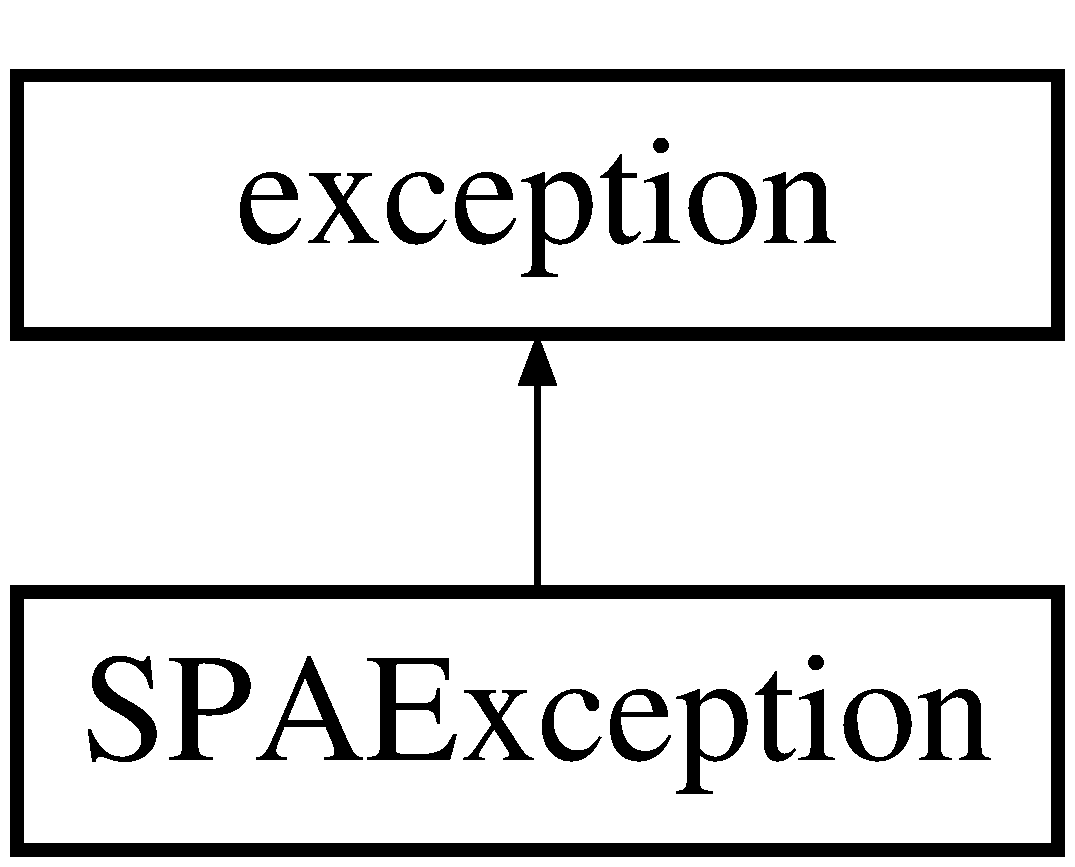
\includegraphics[height=2.000000cm]{class_s_p_a_exception}
\end{center}
\end{figure}
\subsection*{Public Member Functions}
\begin{DoxyCompactItemize}
\item 
\hyperlink{class_s_p_a_exception_a8f17fd2540fce63ba93e51c51765010d}{S\-P\-A\-Exception} ()
\item 
\hyperlink{class_s_p_a_exception_a422623fc7b2c546620c231cf8eebd53b}{S\-P\-A\-Exception} (string)
\item 
virtual const char $\ast$ \hyperlink{class_s_p_a_exception_a968d8912a66e211f71e47a710f5d6667}{what} () const   throw ()
\end{DoxyCompactItemize}
\subsection*{Public Attributes}
\begin{DoxyCompactItemize}
\item 
string \hyperlink{class_s_p_a_exception_a01dacc987941a94c516cb08988dc7d51}{message}
\end{DoxyCompactItemize}


\subsection{Detailed Description}


Definition at line 5 of file S\-P\-A\-Exception.\-h.



\subsection{Constructor \& Destructor Documentation}
\hypertarget{class_s_p_a_exception_a8f17fd2540fce63ba93e51c51765010d}{\index{S\-P\-A\-Exception@{S\-P\-A\-Exception}!S\-P\-A\-Exception@{S\-P\-A\-Exception}}
\index{S\-P\-A\-Exception@{S\-P\-A\-Exception}!SPAException@{S\-P\-A\-Exception}}
\subsubsection[{S\-P\-A\-Exception}]{\setlength{\rightskip}{0pt plus 5cm}S\-P\-A\-Exception\-::\-S\-P\-A\-Exception (
\begin{DoxyParamCaption}
{}
\end{DoxyParamCaption}
)}}\label{class_s_p_a_exception_a8f17fd2540fce63ba93e51c51765010d}
Constructor for \hyperlink{class_s_p_a_exception}{S\-P\-A\-Exception}, a custom exception used for the S\-P\-A program 

Definition at line 8 of file S\-P\-A\-Exception.\-cpp.

\hypertarget{class_s_p_a_exception_a422623fc7b2c546620c231cf8eebd53b}{\index{S\-P\-A\-Exception@{S\-P\-A\-Exception}!S\-P\-A\-Exception@{S\-P\-A\-Exception}}
\index{S\-P\-A\-Exception@{S\-P\-A\-Exception}!SPAException@{S\-P\-A\-Exception}}
\subsubsection[{S\-P\-A\-Exception}]{\setlength{\rightskip}{0pt plus 5cm}S\-P\-A\-Exception\-::\-S\-P\-A\-Exception (
\begin{DoxyParamCaption}
\item[{string}]{msg}
\end{DoxyParamCaption}
)}}\label{class_s_p_a_exception_a422623fc7b2c546620c231cf8eebd53b}
Constructor for \hyperlink{class_s_p_a_exception}{S\-P\-A\-Exception}, a custom exception used for the S\-P\-A program 
\begin{DoxyParams}{Parameters}
{\em msg} & the error message of the Exception \\
\hline
\end{DoxyParams}


Definition at line 16 of file S\-P\-A\-Exception.\-cpp.



\subsection{Member Function Documentation}
\hypertarget{class_s_p_a_exception_a968d8912a66e211f71e47a710f5d6667}{\index{S\-P\-A\-Exception@{S\-P\-A\-Exception}!what@{what}}
\index{what@{what}!SPAException@{S\-P\-A\-Exception}}
\subsubsection[{what}]{\setlength{\rightskip}{0pt plus 5cm}const char $\ast$ S\-P\-A\-Exception\-::what (
\begin{DoxyParamCaption}
{}
\end{DoxyParamCaption}
) const  throw ()\hspace{0.3cm}{\ttfamily [virtual]}}}\label{class_s_p_a_exception_a968d8912a66e211f71e47a710f5d6667}
Returns a null terminated character sequence containing a generic description of the exception. \begin{DoxyReturn}{Returns}
the error message that is thrown 
\end{DoxyReturn}


Definition at line 24 of file S\-P\-A\-Exception.\-cpp.



\subsection{Member Data Documentation}
\hypertarget{class_s_p_a_exception_a01dacc987941a94c516cb08988dc7d51}{\index{S\-P\-A\-Exception@{S\-P\-A\-Exception}!message@{message}}
\index{message@{message}!SPAException@{S\-P\-A\-Exception}}
\subsubsection[{message}]{\setlength{\rightskip}{0pt plus 5cm}string S\-P\-A\-Exception\-::message}}\label{class_s_p_a_exception_a01dacc987941a94c516cb08988dc7d51}


Definition at line 8 of file S\-P\-A\-Exception.\-h.



The documentation for this class was generated from the following files\-:\begin{DoxyCompactItemize}
\item 
\$\-P@/\-S\-P\-A/\-S\-P\-A/\hyperlink{_s_p_a_exception_8h}{S\-P\-A\-Exception.\-h}\item 
\$\-P@/\-S\-P\-A/\-S\-P\-A/\hyperlink{_s_p_a_exception_8cpp}{S\-P\-A\-Exception.\-cpp}\end{DoxyCompactItemize}

\hypertarget{class_synonym_table}{\section{Synonym\-Table Class Reference}
\label{class_synonym_table}\index{Synonym\-Table@{Synonym\-Table}}
}


{\ttfamily \#include $<$Synonym\-Table.\-h$>$}

\subsection*{Public Member Functions}
\begin{DoxyCompactItemize}
\item 
int \hyperlink{class_synonym_table_a4c07332f021c0d969bd913be1bf82bd6}{get\-Size} () const 
\item 
void \hyperlink{class_synonym_table_abda36f6346220b4d99efc9e522f57ac1}{insert} (const string \&name, \hyperlink{class_rules_of_engagement_a5dd2b28fd0c906d9b08e29e371713ead}{Rules\-Of\-Engagement\-::\-Query\-Var} type)
\item 
vector$<$ string $>$ \hyperlink{class_synonym_table_acb150fae4c378832b51b514da7d85bc2}{get\-All\-Names} () const 
\item 
bool \hyperlink{class_synonym_table_aa580c404821e407357fd6cc512504f76}{is\-In\-Table} (const string \&name) const 
\item 
vector$<$ string $>$ \hyperlink{class_synonym_table_ab43bd9f067e43b73afa7c096cb56f07a}{get\-All\-Of\-Type} (\hyperlink{class_rules_of_engagement_a5dd2b28fd0c906d9b08e29e371713ead}{Rules\-Of\-Engagement\-::\-Query\-Var} type) const 
\item 
\hyperlink{class_rules_of_engagement_a5dd2b28fd0c906d9b08e29e371713ead}{Rules\-Of\-Engagement\-::\-Query\-Var} \hyperlink{class_synonym_table_abda3f936a0e70d91ae26470c6a1b902a}{get\-Type} (const string \&) const 
\item 
int \hyperlink{class_synonym_table_a040c55f27a2f9c23aedf6818c40324df}{get\-Synonym\-Index} (const string \&name) const 
\item 
void \hyperlink{class_synonym_table_a57707788e5729fcb3edb8c17d56ea056}{set\-Selected} (const string \&name)
\item 
vector$<$ string $>$ \hyperlink{class_synonym_table_a10082dabe233a4cc136012604fdd0c99}{get\-All\-Selected} () const 
\item 
bool \hyperlink{class_synonym_table_aedd2ee139a4bea5ebff46e0e795b303f}{is\-Selected} (const string \&name) const 
\item 
void \hyperlink{class_synonym_table_a2f84ea7622341e430ccef2fe54cd0493}{put\-Into\-Class} (const string \&name, int class\-Index)
\item 
int \hyperlink{class_synonym_table_ae9aefbf36f2f08661aff39d903f4d4e9}{get\-Class} (const string \&name) const 
\item 
bool \hyperlink{class_synonym_table_aedd5d18cb3c7f31827142e52b76f725a}{set\-Specific\-Attribute} (const string \&name, const string \&condition, const string \&attribute)
\item 
unordered\-\_\-map$<$ string, string $>$ \hyperlink{class_synonym_table_aae3ea3b80a7c9d8527299bb709da36e7}{get\-All\-Specific\-Attributes} (const string \&name) const 
\item 
void \hyperlink{class_synonym_table_aa3939003680ee31c93b61adb82e5e407}{set\-Generic\-Attribute} (const string \&name, const string \&own\-Attribute, \hyperlink{class_rules_of_engagement_a5dd2b28fd0c906d9b08e29e371713ead}{Rules\-Of\-Engagement\-::\-Query\-Var} other\-Variable, const string \&other\-Attribute)
\item 
unordered\-\_\-map$<$ string, \\*
unordered\-\_\-map\\*
$<$ \hyperlink{class_rules_of_engagement_a5dd2b28fd0c906d9b08e29e371713ead}{Rules\-Of\-Engagement\-::\-Query\-Var}, \\*
string $>$ $>$ \hyperlink{class_synonym_table_a24fafd4eef36373854f0552639d1a23a}{get\-All\-Generic\-Attributes} (const string \&name) const 
\item 
void \hyperlink{class_synonym_table_a394f3fe82c0e8908e531fed0353a043b}{set\-Self\-Reference} (const string \&name, \hyperlink{class_rules_of_engagement_a5e08db2a0638b98dbb06ad923a33d817}{Rules\-Of\-Engagement\-::\-Query\-Relations} relation)
\item 
unordered\-\_\-set\\*
$<$ \hyperlink{class_rules_of_engagement_a5e08db2a0638b98dbb06ad923a33d817}{Rules\-Of\-Engagement\-::\-Query\-Relations} $>$ \hyperlink{class_synonym_table_a644d28f9dc3c765572a83c98cf75b66d}{get\-All\-Self\-References} (const string \&name) const 
\item 
void \hyperlink{class_synonym_table_ad53932d85419c69ff93db7a0b094791b}{set\-First\-Generic} (const string \&name, \hyperlink{class_rules_of_engagement_a5e08db2a0638b98dbb06ad923a33d817}{Rules\-Of\-Engagement\-::\-Query\-Relations} relation)
\item 
unordered\-\_\-set\\*
$<$ \hyperlink{class_rules_of_engagement_a5e08db2a0638b98dbb06ad923a33d817}{Rules\-Of\-Engagement\-::\-Query\-Relations} $>$ \hyperlink{class_synonym_table_a6fd51931d0f5a80722fdd74dddbc6b68}{get\-All\-First\-Generic} (const string \&name) const 
\item 
void \hyperlink{class_synonym_table_a55b56ddfb36fe07ec341d470da958401}{set\-First\-Specific} (const string \&name, \hyperlink{class_rules_of_engagement_a5e08db2a0638b98dbb06ad923a33d817}{Rules\-Of\-Engagement\-::\-Query\-Relations} relation, const string \&specific)
\item 
vector$<$ pair\\*
$<$ \hyperlink{class_rules_of_engagement_a5e08db2a0638b98dbb06ad923a33d817}{Rules\-Of\-Engagement\-::\-Query\-Relations}, \\*
string $>$ $>$ \hyperlink{class_synonym_table_af223b1e48694ef48618a60753cf4d163}{get\-All\-First\-Specific} (const string \&name) const 
\item 
void \hyperlink{class_synonym_table_a163973b15f35deae030c1b194a06c1a2}{set\-Second\-Generic} (const string \&name, \hyperlink{class_rules_of_engagement_a5e08db2a0638b98dbb06ad923a33d817}{Rules\-Of\-Engagement\-::\-Query\-Relations} relation)
\item 
unordered\-\_\-set\\*
$<$ \hyperlink{class_rules_of_engagement_a5e08db2a0638b98dbb06ad923a33d817}{Rules\-Of\-Engagement\-::\-Query\-Relations} $>$ \hyperlink{class_synonym_table_aab6e5790402227ff0f28fe93fdc9d24f}{get\-All\-Second\-Generic} (const string \&name) const 
\item 
void \hyperlink{class_synonym_table_afd36238b0cd5ace74c15dfe30a302670}{set\-Second\-Specific} (const string \&name, \hyperlink{class_rules_of_engagement_a5e08db2a0638b98dbb06ad923a33d817}{Rules\-Of\-Engagement\-::\-Query\-Relations} relation, const string \&specific)
\item 
vector$<$ pair\\*
$<$ \hyperlink{class_rules_of_engagement_a5e08db2a0638b98dbb06ad923a33d817}{Rules\-Of\-Engagement\-::\-Query\-Relations}, \\*
string $>$ $>$ \hyperlink{class_synonym_table_a4e0c4cdc09a90edb32b1af4bc26172d6}{get\-All\-Second\-Specific} (const string \&name) const 
\end{DoxyCompactItemize}


\subsection{Detailed Description}


Definition at line 5 of file Synonym\-Table.\-h.



\subsection{Member Function Documentation}
\hypertarget{class_synonym_table_a6fd51931d0f5a80722fdd74dddbc6b68}{\index{Synonym\-Table@{Synonym\-Table}!get\-All\-First\-Generic@{get\-All\-First\-Generic}}
\index{get\-All\-First\-Generic@{get\-All\-First\-Generic}!SynonymTable@{Synonym\-Table}}
\subsubsection[{get\-All\-First\-Generic}]{\setlength{\rightskip}{0pt plus 5cm}unordered\-\_\-set$<$ {\bf Rules\-Of\-Engagement\-::\-Query\-Relations} $>$ Synonym\-Table\-::get\-All\-First\-Generic (
\begin{DoxyParamCaption}
\item[{const string \&}]{name}
\end{DoxyParamCaption}
) const}}\label{class_synonym_table_a6fd51931d0f5a80722fdd74dddbc6b68}
This method Returns all generic conditions (synonym is first argument) on the synonym. 
\begin{DoxyParams}{Parameters}
{\em name} & name of own synonym \\
\hline
\end{DoxyParams}
\begin{DoxyReturn}{Returns}
an unordered set containing all the generic conditions (synonym is first argument) 
\end{DoxyReturn}


Definition at line 251 of file Synonym\-Table.\-cpp.

\hypertarget{class_synonym_table_af223b1e48694ef48618a60753cf4d163}{\index{Synonym\-Table@{Synonym\-Table}!get\-All\-First\-Specific@{get\-All\-First\-Specific}}
\index{get\-All\-First\-Specific@{get\-All\-First\-Specific}!SynonymTable@{Synonym\-Table}}
\subsubsection[{get\-All\-First\-Specific}]{\setlength{\rightskip}{0pt plus 5cm}vector$<$ pair$<$ {\bf Rules\-Of\-Engagement\-::\-Query\-Relations}, string $>$ $>$ Synonym\-Table\-::get\-All\-First\-Specific (
\begin{DoxyParamCaption}
\item[{const string \&}]{name}
\end{DoxyParamCaption}
) const}}\label{class_synonym_table_af223b1e48694ef48618a60753cf4d163}
This method Returns all specific conditions (synonym is first argument) on the synonym. 
\begin{DoxyParams}{Parameters}
{\em name} & name of own synonym \\
\hline
\end{DoxyParams}
\begin{DoxyReturn}{Returns}
an unordered set containing all the specific conditions (synonym is first argument) 
\end{DoxyReturn}


Definition at line 275 of file Synonym\-Table.\-cpp.

\hypertarget{class_synonym_table_a24fafd4eef36373854f0552639d1a23a}{\index{Synonym\-Table@{Synonym\-Table}!get\-All\-Generic\-Attributes@{get\-All\-Generic\-Attributes}}
\index{get\-All\-Generic\-Attributes@{get\-All\-Generic\-Attributes}!SynonymTable@{Synonym\-Table}}
\subsubsection[{get\-All\-Generic\-Attributes}]{\setlength{\rightskip}{0pt plus 5cm}unordered\-\_\-map$<$ string, unordered\-\_\-map$<$ {\bf Rules\-Of\-Engagement\-::\-Query\-Var}, string $>$ $>$ Synonym\-Table\-::get\-All\-Generic\-Attributes (
\begin{DoxyParamCaption}
\item[{const string \&}]{name}
\end{DoxyParamCaption}
) const}}\label{class_synonym_table_a24fafd4eef36373854f0552639d1a23a}
This method Returns all generic conditions on the synonym. 
\begin{DoxyParams}{Parameters}
{\em name} & name of own synonym \\
\hline
\end{DoxyParams}
\begin{DoxyReturn}{Returns}
an unordered map containing all the generic conditions 
\end{DoxyReturn}


Definition at line 207 of file Synonym\-Table.\-cpp.

\hypertarget{class_synonym_table_acb150fae4c378832b51b514da7d85bc2}{\index{Synonym\-Table@{Synonym\-Table}!get\-All\-Names@{get\-All\-Names}}
\index{get\-All\-Names@{get\-All\-Names}!SynonymTable@{Synonym\-Table}}
\subsubsection[{get\-All\-Names}]{\setlength{\rightskip}{0pt plus 5cm}vector$<$ string $>$ Synonym\-Table\-::get\-All\-Names (
\begin{DoxyParamCaption}
{}
\end{DoxyParamCaption}
) const}}\label{class_synonym_table_acb150fae4c378832b51b514da7d85bc2}
This method Returns a vector of all synonyms in \hyperlink{class_synonym_table}{Synonym\-Table}. \begin{DoxyReturn}{Returns}
the vector 
\end{DoxyReturn}


Definition at line 54 of file Synonym\-Table.\-cpp.

\hypertarget{class_synonym_table_ab43bd9f067e43b73afa7c096cb56f07a}{\index{Synonym\-Table@{Synonym\-Table}!get\-All\-Of\-Type@{get\-All\-Of\-Type}}
\index{get\-All\-Of\-Type@{get\-All\-Of\-Type}!SynonymTable@{Synonym\-Table}}
\subsubsection[{get\-All\-Of\-Type}]{\setlength{\rightskip}{0pt plus 5cm}vector$<$ string $>$ Synonym\-Table\-::get\-All\-Of\-Type (
\begin{DoxyParamCaption}
\item[{{\bf Rules\-Of\-Engagement\-::\-Query\-Var}}]{type}
\end{DoxyParamCaption}
) const}}\label{class_synonym_table_ab43bd9f067e43b73afa7c096cb56f07a}
This method Returns a vector of all synonyms of the given type. 
\begin{DoxyParams}{Parameters}
{\em type} & type of variable \\
\hline
\end{DoxyParams}
\begin{DoxyReturn}{Returns}
the vector 
\end{DoxyReturn}


Definition at line 74 of file Synonym\-Table.\-cpp.

\hypertarget{class_synonym_table_aab6e5790402227ff0f28fe93fdc9d24f}{\index{Synonym\-Table@{Synonym\-Table}!get\-All\-Second\-Generic@{get\-All\-Second\-Generic}}
\index{get\-All\-Second\-Generic@{get\-All\-Second\-Generic}!SynonymTable@{Synonym\-Table}}
\subsubsection[{get\-All\-Second\-Generic}]{\setlength{\rightskip}{0pt plus 5cm}unordered\-\_\-set$<$ {\bf Rules\-Of\-Engagement\-::\-Query\-Relations} $>$ Synonym\-Table\-::get\-All\-Second\-Generic (
\begin{DoxyParamCaption}
\item[{const string \&}]{name}
\end{DoxyParamCaption}
) const}}\label{class_synonym_table_aab6e5790402227ff0f28fe93fdc9d24f}
This method Returns all generic conditions (synonym is second argument) on the synonym. 
\begin{DoxyParams}{Parameters}
{\em name} & name of own synonym \\
\hline
\end{DoxyParams}
\begin{DoxyReturn}{Returns}
an unordered set containing all the generic conditions (synonym is second argument) 
\end{DoxyReturn}


Definition at line 297 of file Synonym\-Table.\-cpp.

\hypertarget{class_synonym_table_a4e0c4cdc09a90edb32b1af4bc26172d6}{\index{Synonym\-Table@{Synonym\-Table}!get\-All\-Second\-Specific@{get\-All\-Second\-Specific}}
\index{get\-All\-Second\-Specific@{get\-All\-Second\-Specific}!SynonymTable@{Synonym\-Table}}
\subsubsection[{get\-All\-Second\-Specific}]{\setlength{\rightskip}{0pt plus 5cm}vector$<$ pair$<$ {\bf Rules\-Of\-Engagement\-::\-Query\-Relations}, string $>$ $>$ Synonym\-Table\-::get\-All\-Second\-Specific (
\begin{DoxyParamCaption}
\item[{const string \&}]{name}
\end{DoxyParamCaption}
) const}}\label{class_synonym_table_a4e0c4cdc09a90edb32b1af4bc26172d6}
This method Returns all specific conditions (synonym is second argument) on the synonym. 
\begin{DoxyParams}{Parameters}
{\em name} & name of own synonym \\
\hline
\end{DoxyParams}
\begin{DoxyReturn}{Returns}
an unordered set containing all the specific conditions (synonym is second argument) 
\end{DoxyReturn}


Definition at line 321 of file Synonym\-Table.\-cpp.

\hypertarget{class_synonym_table_a10082dabe233a4cc136012604fdd0c99}{\index{Synonym\-Table@{Synonym\-Table}!get\-All\-Selected@{get\-All\-Selected}}
\index{get\-All\-Selected@{get\-All\-Selected}!SynonymTable@{Synonym\-Table}}
\subsubsection[{get\-All\-Selected}]{\setlength{\rightskip}{0pt plus 5cm}vector$<$ string $>$ Synonym\-Table\-::get\-All\-Selected (
\begin{DoxyParamCaption}
{}
\end{DoxyParamCaption}
) const}}\label{class_synonym_table_a10082dabe233a4cc136012604fdd0c99}
This method Returns a vector of all selected for synonyms. \begin{DoxyReturn}{Returns}
the vector 
\end{DoxyReturn}


Definition at line 117 of file Synonym\-Table.\-cpp.

\hypertarget{class_synonym_table_a644d28f9dc3c765572a83c98cf75b66d}{\index{Synonym\-Table@{Synonym\-Table}!get\-All\-Self\-References@{get\-All\-Self\-References}}
\index{get\-All\-Self\-References@{get\-All\-Self\-References}!SynonymTable@{Synonym\-Table}}
\subsubsection[{get\-All\-Self\-References}]{\setlength{\rightskip}{0pt plus 5cm}unordered\-\_\-set$<$ {\bf Rules\-Of\-Engagement\-::\-Query\-Relations} $>$ Synonym\-Table\-::get\-All\-Self\-References (
\begin{DoxyParamCaption}
\item[{const string \&}]{name}
\end{DoxyParamCaption}
) const}}\label{class_synonym_table_a644d28f9dc3c765572a83c98cf75b66d}
This method Returns all self references on the synonym. 
\begin{DoxyParams}{Parameters}
{\em name} & name of own synonym \\
\hline
\end{DoxyParams}
\begin{DoxyReturn}{Returns}
an unordered set containing all the self references 
\end{DoxyReturn}


Definition at line 229 of file Synonym\-Table.\-cpp.

\hypertarget{class_synonym_table_aae3ea3b80a7c9d8527299bb709da36e7}{\index{Synonym\-Table@{Synonym\-Table}!get\-All\-Specific\-Attributes@{get\-All\-Specific\-Attributes}}
\index{get\-All\-Specific\-Attributes@{get\-All\-Specific\-Attributes}!SynonymTable@{Synonym\-Table}}
\subsubsection[{get\-All\-Specific\-Attributes}]{\setlength{\rightskip}{0pt plus 5cm}unordered\-\_\-map$<$ string, string $>$ Synonym\-Table\-::get\-All\-Specific\-Attributes (
\begin{DoxyParamCaption}
\item[{const string \&}]{name}
\end{DoxyParamCaption}
) const}}\label{class_synonym_table_aae3ea3b80a7c9d8527299bb709da36e7}
This method Returns all specific conditions on the synonym. 
\begin{DoxyParams}{Parameters}
{\em name} & name of synonym \\
\hline
\end{DoxyParams}
\begin{DoxyReturn}{Returns}
an unordered map containing all the specific conditions 
\end{DoxyReturn}


Definition at line 180 of file Synonym\-Table.\-cpp.

\hypertarget{class_synonym_table_ae9aefbf36f2f08661aff39d903f4d4e9}{\index{Synonym\-Table@{Synonym\-Table}!get\-Class@{get\-Class}}
\index{get\-Class@{get\-Class}!SynonymTable@{Synonym\-Table}}
\subsubsection[{get\-Class}]{\setlength{\rightskip}{0pt plus 5cm}int Synonym\-Table\-::get\-Class (
\begin{DoxyParamCaption}
\item[{const string \&}]{name}
\end{DoxyParamCaption}
) const}}\label{class_synonym_table_ae9aefbf36f2f08661aff39d903f4d4e9}
This method Returns the partition that the given synonym is in. 
\begin{DoxyParams}{Parameters}
{\em name} & name of synonym \\
\hline
\end{DoxyParams}
\begin{DoxyReturn}{Returns}
the partition 
\end{DoxyReturn}


Definition at line 150 of file Synonym\-Table.\-cpp.

\hypertarget{class_synonym_table_a4c07332f021c0d969bd913be1bf82bd6}{\index{Synonym\-Table@{Synonym\-Table}!get\-Size@{get\-Size}}
\index{get\-Size@{get\-Size}!SynonymTable@{Synonym\-Table}}
\subsubsection[{get\-Size}]{\setlength{\rightskip}{0pt plus 5cm}int Synonym\-Table\-::get\-Size (
\begin{DoxyParamCaption}
{}
\end{DoxyParamCaption}
) const}}\label{class_synonym_table_a4c07332f021c0d969bd913be1bf82bd6}
This method Returns the number of synonyms in the \hyperlink{class_synonym_table}{Synonym\-Table} \begin{DoxyReturn}{Returns}
the number of synonyms 
\end{DoxyReturn}


Definition at line 9 of file Synonym\-Table.\-cpp.

\hypertarget{class_synonym_table_a040c55f27a2f9c23aedf6818c40324df}{\index{Synonym\-Table@{Synonym\-Table}!get\-Synonym\-Index@{get\-Synonym\-Index}}
\index{get\-Synonym\-Index@{get\-Synonym\-Index}!SynonymTable@{Synonym\-Table}}
\subsubsection[{get\-Synonym\-Index}]{\setlength{\rightskip}{0pt plus 5cm}int Synonym\-Table\-::get\-Synonym\-Index (
\begin{DoxyParamCaption}
\item[{const string \&}]{name}
\end{DoxyParamCaption}
) const}}\label{class_synonym_table_a040c55f27a2f9c23aedf6818c40324df}
This method Returns the index in the \hyperlink{class_synonym_table}{Synonym\-Table}, of the given synonym. 
\begin{DoxyParams}{Parameters}
{\em name} & name of synonym \\
\hline
\end{DoxyParams}
\begin{DoxyReturn}{Returns}
the index 
\end{DoxyReturn}


Definition at line 98 of file Synonym\-Table.\-cpp.

\hypertarget{class_synonym_table_abda3f936a0e70d91ae26470c6a1b902a}{\index{Synonym\-Table@{Synonym\-Table}!get\-Type@{get\-Type}}
\index{get\-Type@{get\-Type}!SynonymTable@{Synonym\-Table}}
\subsubsection[{get\-Type}]{\setlength{\rightskip}{0pt plus 5cm}{\bf Rules\-Of\-Engagement\-::\-Query\-Var} Synonym\-Table\-::get\-Type (
\begin{DoxyParamCaption}
\item[{const string \&}]{name}
\end{DoxyParamCaption}
) const}}\label{class_synonym_table_abda3f936a0e70d91ae26470c6a1b902a}
This method Returns the type of the given synonym. 
\begin{DoxyParams}{Parameters}
{\em name} & name of synonym \\
\hline
\end{DoxyParams}
\begin{DoxyReturn}{Returns}
the type 
\end{DoxyReturn}


Definition at line 88 of file Synonym\-Table.\-cpp.

\hypertarget{class_synonym_table_abda36f6346220b4d99efc9e522f57ac1}{\index{Synonym\-Table@{Synonym\-Table}!insert@{insert}}
\index{insert@{insert}!SynonymTable@{Synonym\-Table}}
\subsubsection[{insert}]{\setlength{\rightskip}{0pt plus 5cm}void Synonym\-Table\-::insert (
\begin{DoxyParamCaption}
\item[{const string \&}]{name, }
\item[{{\bf Rules\-Of\-Engagement\-::\-Query\-Var}}]{type}
\end{DoxyParamCaption}
)}}\label{class_synonym_table_abda36f6346220b4d99efc9e522f57ac1}
This method Inserts the synonym in the \hyperlink{class_synonym_table}{Synonym\-Table} if it is not already present. 
\begin{DoxyParams}{Parameters}
{\em name} & name of synonym \\
\hline
{\em type} & type of variable \\
\hline
\end{DoxyParams}


Definition at line 19 of file Synonym\-Table.\-cpp.

\hypertarget{class_synonym_table_aa580c404821e407357fd6cc512504f76}{\index{Synonym\-Table@{Synonym\-Table}!is\-In\-Table@{is\-In\-Table}}
\index{is\-In\-Table@{is\-In\-Table}!SynonymTable@{Synonym\-Table}}
\subsubsection[{is\-In\-Table}]{\setlength{\rightskip}{0pt plus 5cm}bool Synonym\-Table\-::is\-In\-Table (
\begin{DoxyParamCaption}
\item[{const string \&}]{name}
\end{DoxyParamCaption}
) const}}\label{class_synonym_table_aa580c404821e407357fd6cc512504f76}
This method Returns true if the synonym is in \hyperlink{class_synonym_table}{Synonym\-Table}. 
\begin{DoxyParams}{Parameters}
{\em name} & name of synonym \\
\hline
\end{DoxyParams}
\begin{DoxyReturn}{Returns}
true if the synonym is in \hyperlink{class_synonym_table}{Synonym\-Table}, and false otherwise. 
\end{DoxyReturn}


Definition at line 64 of file Synonym\-Table.\-cpp.

\hypertarget{class_synonym_table_aedd2ee139a4bea5ebff46e0e795b303f}{\index{Synonym\-Table@{Synonym\-Table}!is\-Selected@{is\-Selected}}
\index{is\-Selected@{is\-Selected}!SynonymTable@{Synonym\-Table}}
\subsubsection[{is\-Selected}]{\setlength{\rightskip}{0pt plus 5cm}bool Synonym\-Table\-::is\-Selected (
\begin{DoxyParamCaption}
\item[{const string \&}]{name}
\end{DoxyParamCaption}
) const}}\label{class_synonym_table_aedd2ee139a4bea5ebff46e0e795b303f}
This method Returns true if the given synonym is selected for. 
\begin{DoxyParams}{Parameters}
{\em name} & name of synonym \\
\hline
\end{DoxyParams}
\begin{DoxyReturn}{Returns}
true if the synonym is selected for, and false otherwise. 
\end{DoxyReturn}


Definition at line 130 of file Synonym\-Table.\-cpp.

\hypertarget{class_synonym_table_a2f84ea7622341e430ccef2fe54cd0493}{\index{Synonym\-Table@{Synonym\-Table}!put\-Into\-Class@{put\-Into\-Class}}
\index{put\-Into\-Class@{put\-Into\-Class}!SynonymTable@{Synonym\-Table}}
\subsubsection[{put\-Into\-Class}]{\setlength{\rightskip}{0pt plus 5cm}void Synonym\-Table\-::put\-Into\-Class (
\begin{DoxyParamCaption}
\item[{const string \&}]{name, }
\item[{int}]{class\-Index}
\end{DoxyParamCaption}
)}}\label{class_synonym_table_a2f84ea7622341e430ccef2fe54cd0493}
This method Sets the partition that the given synonym is in. 
\begin{DoxyParams}{Parameters}
{\em name} & name of synonym \\
\hline
{\em class\-Index} & index of the partition \\
\hline
\end{DoxyParams}


Definition at line 140 of file Synonym\-Table.\-cpp.

\hypertarget{class_synonym_table_ad53932d85419c69ff93db7a0b094791b}{\index{Synonym\-Table@{Synonym\-Table}!set\-First\-Generic@{set\-First\-Generic}}
\index{set\-First\-Generic@{set\-First\-Generic}!SynonymTable@{Synonym\-Table}}
\subsubsection[{set\-First\-Generic}]{\setlength{\rightskip}{0pt plus 5cm}void Synonym\-Table\-::set\-First\-Generic (
\begin{DoxyParamCaption}
\item[{const string \&}]{name, }
\item[{{\bf Rules\-Of\-Engagement\-::\-Query\-Relations}}]{relation}
\end{DoxyParamCaption}
)}}\label{class_synonym_table_ad53932d85419c69ff93db7a0b094791b}
This method Sets a generic condition on the synonym (first argument). It must be of the form relation(name, \-\_\-). 
\begin{DoxyParams}{Parameters}
{\em name} & name of own synonym \\
\hline
{\em relation} & type of variable \\
\hline
\end{DoxyParams}


Definition at line 239 of file Synonym\-Table.\-cpp.

\hypertarget{class_synonym_table_a55b56ddfb36fe07ec341d470da958401}{\index{Synonym\-Table@{Synonym\-Table}!set\-First\-Specific@{set\-First\-Specific}}
\index{set\-First\-Specific@{set\-First\-Specific}!SynonymTable@{Synonym\-Table}}
\subsubsection[{set\-First\-Specific}]{\setlength{\rightskip}{0pt plus 5cm}void Synonym\-Table\-::set\-First\-Specific (
\begin{DoxyParamCaption}
\item[{const string \&}]{name, }
\item[{{\bf Rules\-Of\-Engagement\-::\-Query\-Relations}}]{relation, }
\item[{const string \&}]{specific}
\end{DoxyParamCaption}
)}}\label{class_synonym_table_a55b56ddfb36fe07ec341d470da958401}
This method Sets a specific condition on the synonym (first argument). It must be of the form relation(name, specific). 
\begin{DoxyParams}{Parameters}
{\em name} & name of own synonym \\
\hline
{\em relation} & type of variable \\
\hline
{\em specific} & the specific attribute \\
\hline
\end{DoxyParams}


Definition at line 263 of file Synonym\-Table.\-cpp.

\hypertarget{class_synonym_table_aa3939003680ee31c93b61adb82e5e407}{\index{Synonym\-Table@{Synonym\-Table}!set\-Generic\-Attribute@{set\-Generic\-Attribute}}
\index{set\-Generic\-Attribute@{set\-Generic\-Attribute}!SynonymTable@{Synonym\-Table}}
\subsubsection[{set\-Generic\-Attribute}]{\setlength{\rightskip}{0pt plus 5cm}void Synonym\-Table\-::set\-Generic\-Attribute (
\begin{DoxyParamCaption}
\item[{const string \&}]{name, }
\item[{const string \&}]{own\-Attribute, }
\item[{{\bf Rules\-Of\-Engagement\-::\-Query\-Var}}]{other\-Variable, }
\item[{const string \&}]{other\-Attribute}
\end{DoxyParamCaption}
)}}\label{class_synonym_table_aa3939003680ee31c93b61adb82e5e407}
This method Sets a generic condition on the synonym. It must be of the form name.\-own\-Attribute = type.\-attribute 
\begin{DoxyParams}{Parameters}
{\em name} & name of own synonym \\
\hline
{\em own\-Attribute} & name of own attribute \\
\hline
{\em other\-Variable} & name of other synonym \\
\hline
{\em other\-Attribute} & name of other attribute \\
\hline
\end{DoxyParams}


Definition at line 192 of file Synonym\-Table.\-cpp.

\hypertarget{class_synonym_table_a163973b15f35deae030c1b194a06c1a2}{\index{Synonym\-Table@{Synonym\-Table}!set\-Second\-Generic@{set\-Second\-Generic}}
\index{set\-Second\-Generic@{set\-Second\-Generic}!SynonymTable@{Synonym\-Table}}
\subsubsection[{set\-Second\-Generic}]{\setlength{\rightskip}{0pt plus 5cm}void Synonym\-Table\-::set\-Second\-Generic (
\begin{DoxyParamCaption}
\item[{const string \&}]{name, }
\item[{{\bf Rules\-Of\-Engagement\-::\-Query\-Relations}}]{relation}
\end{DoxyParamCaption}
)}}\label{class_synonym_table_a163973b15f35deae030c1b194a06c1a2}
This method Sets a generic condition on the synonym (second argument). It must be of the form relation(\-\_\-, name). 
\begin{DoxyParams}{Parameters}
{\em name} & name of own synonym \\
\hline
{\em relation} & type of variable \\
\hline
\end{DoxyParams}


Definition at line 285 of file Synonym\-Table.\-cpp.

\hypertarget{class_synonym_table_afd36238b0cd5ace74c15dfe30a302670}{\index{Synonym\-Table@{Synonym\-Table}!set\-Second\-Specific@{set\-Second\-Specific}}
\index{set\-Second\-Specific@{set\-Second\-Specific}!SynonymTable@{Synonym\-Table}}
\subsubsection[{set\-Second\-Specific}]{\setlength{\rightskip}{0pt plus 5cm}void Synonym\-Table\-::set\-Second\-Specific (
\begin{DoxyParamCaption}
\item[{const string \&}]{name, }
\item[{{\bf Rules\-Of\-Engagement\-::\-Query\-Relations}}]{relation, }
\item[{const string \&}]{specific}
\end{DoxyParamCaption}
)}}\label{class_synonym_table_afd36238b0cd5ace74c15dfe30a302670}
This method Sets a specific condition on the synonym (second argument). It must be of the form relation(specific, name). 
\begin{DoxyParams}{Parameters}
{\em name} & name of own synonym \\
\hline
{\em relation} & type of variable \\
\hline
{\em specific} & the specific attribute \\
\hline
\end{DoxyParams}


Definition at line 309 of file Synonym\-Table.\-cpp.

\hypertarget{class_synonym_table_a57707788e5729fcb3edb8c17d56ea056}{\index{Synonym\-Table@{Synonym\-Table}!set\-Selected@{set\-Selected}}
\index{set\-Selected@{set\-Selected}!SynonymTable@{Synonym\-Table}}
\subsubsection[{set\-Selected}]{\setlength{\rightskip}{0pt plus 5cm}void Synonym\-Table\-::set\-Selected (
\begin{DoxyParamCaption}
\item[{const string \&}]{name}
\end{DoxyParamCaption}
)}}\label{class_synonym_table_a57707788e5729fcb3edb8c17d56ea056}
This method Sets the synonym as one that is selected for. 
\begin{DoxyParams}{Parameters}
{\em name} & name of synonym \\
\hline
\end{DoxyParams}


Definition at line 107 of file Synonym\-Table.\-cpp.

\hypertarget{class_synonym_table_a394f3fe82c0e8908e531fed0353a043b}{\index{Synonym\-Table@{Synonym\-Table}!set\-Self\-Reference@{set\-Self\-Reference}}
\index{set\-Self\-Reference@{set\-Self\-Reference}!SynonymTable@{Synonym\-Table}}
\subsubsection[{set\-Self\-Reference}]{\setlength{\rightskip}{0pt plus 5cm}void Synonym\-Table\-::set\-Self\-Reference (
\begin{DoxyParamCaption}
\item[{const string \&}]{name, }
\item[{{\bf Rules\-Of\-Engagement\-::\-Query\-Relations}}]{relation}
\end{DoxyParamCaption}
)}}\label{class_synonym_table_a394f3fe82c0e8908e531fed0353a043b}
This method Sets a self reference condition on the synonym. It must be of the form relation(name, name). 
\begin{DoxyParams}{Parameters}
{\em name} & name of own synonym \\
\hline
{\em relation} & type of variable \\
\hline
\end{DoxyParams}


Definition at line 217 of file Synonym\-Table.\-cpp.

\hypertarget{class_synonym_table_aedd5d18cb3c7f31827142e52b76f725a}{\index{Synonym\-Table@{Synonym\-Table}!set\-Specific\-Attribute@{set\-Specific\-Attribute}}
\index{set\-Specific\-Attribute@{set\-Specific\-Attribute}!SynonymTable@{Synonym\-Table}}
\subsubsection[{set\-Specific\-Attribute}]{\setlength{\rightskip}{0pt plus 5cm}bool Synonym\-Table\-::set\-Specific\-Attribute (
\begin{DoxyParamCaption}
\item[{const string \&}]{name, }
\item[{const string \&}]{condition, }
\item[{const string \&}]{attribute}
\end{DoxyParamCaption}
)}}\label{class_synonym_table_aedd5d18cb3c7f31827142e52b76f725a}
This method Sets a specific condition on the synonym. It must be of the form name.\-condition = attribute. 
\begin{DoxyParams}{Parameters}
{\em name} & name of synonym \\
\hline
{\em condition} & name of condition \\
\hline
{\em attribute} & name of attribute \\
\hline
\end{DoxyParams}
\begin{DoxyReturn}{Returns}
true if the condition has not been set before, and false otherwise. 
\end{DoxyReturn}


Definition at line 162 of file Synonym\-Table.\-cpp.



The documentation for this class was generated from the following files\-:\begin{DoxyCompactItemize}
\item 
\$\-P@/\-S\-P\-A/\-S\-P\-A/\hyperlink{_synonym_table_8h}{Synonym\-Table.\-h}\item 
\$\-P@/\-S\-P\-A/\-S\-P\-A/\hyperlink{_synonym_table_8cpp}{Synonym\-Table.\-cpp}\end{DoxyCompactItemize}

\hypertarget{class_uses_table}{\section{Uses\-Table Class Reference}
\label{class_uses_table}\index{Uses\-Table@{Uses\-Table}}
}


{\ttfamily \#include $<$Uses\-Table.\-h$>$}

\subsection*{Public Member Functions}
\begin{DoxyCompactItemize}
\item 
\hyperlink{class_uses_table_a22b7102c56cfa8e9fa4d806c3ad4c586}{Uses\-Table} ()
\item 
void \hyperlink{class_uses_table_ae29b8e5db64f12f6966916c62d4f911b}{insert\-Stmt\-Uses} (\hyperlink{std_afx_8h_a4a876b28ac3f59cecb39c2d2d76e4e7a}{S\-T\-M\-T}, \hyperlink{std_afx_8h_a3112e3faf0465bb5d85272a347b7f2f1}{V\-A\-R})
\item 
void \hyperlink{class_uses_table_a6d7e75d504e79223fa6f9676fb81963a}{insert\-Proc\-Uses} (\hyperlink{std_afx_8h_aa07ea1d188c7b45668f1bd82ffd6d87e}{P\-R\-O\-C}, \hyperlink{std_afx_8h_a3112e3faf0465bb5d85272a347b7f2f1}{V\-A\-R})
\item 
vector$<$ \hyperlink{std_afx_8h_a3112e3faf0465bb5d85272a347b7f2f1}{V\-A\-R} $>$ \hyperlink{class_uses_table_ae6da24dd1e776a415bb74255635b1731}{get\-Used\-By\-Stmt} (\hyperlink{std_afx_8h_a4a876b28ac3f59cecb39c2d2d76e4e7a}{S\-T\-M\-T})
\item 
vector$<$ \hyperlink{std_afx_8h_a3112e3faf0465bb5d85272a347b7f2f1}{V\-A\-R} $>$ \hyperlink{class_uses_table_a606a8c1dc8c9cc3b783e765c09e6891a}{get\-Used\-By\-Proc} (\hyperlink{std_afx_8h_aa07ea1d188c7b45668f1bd82ffd6d87e}{P\-R\-O\-C})
\item 
vector$<$ \hyperlink{std_afx_8h_a4a876b28ac3f59cecb39c2d2d76e4e7a}{S\-T\-M\-T} $>$ \hyperlink{class_uses_table_ae9bc0a7a3183df114286107f0ad72b8b}{get\-Used\-In\-Stmt} (\hyperlink{std_afx_8h_a3112e3faf0465bb5d85272a347b7f2f1}{V\-A\-R})
\item 
vector$<$ \hyperlink{std_afx_8h_aa07ea1d188c7b45668f1bd82ffd6d87e}{P\-R\-O\-C} $>$ \hyperlink{class_uses_table_aaedcc22a6cb307cb6c851e7c64815371}{get\-Used\-In\-Proc} (\hyperlink{std_afx_8h_a3112e3faf0465bb5d85272a347b7f2f1}{V\-A\-R})
\item 
bool \hyperlink{class_uses_table_a0efe799acfbeea3b597258408896ca12}{is\-Used\-Stmt} (\hyperlink{std_afx_8h_a4a876b28ac3f59cecb39c2d2d76e4e7a}{S\-T\-M\-T}, \hyperlink{std_afx_8h_a3112e3faf0465bb5d85272a347b7f2f1}{V\-A\-R})
\item 
bool \hyperlink{class_uses_table_a53a4e37ac552ca2d7b8c7cfc56d3b3db}{is\-Used\-Proc} (\hyperlink{std_afx_8h_aa07ea1d188c7b45668f1bd82ffd6d87e}{P\-R\-O\-C}, \hyperlink{std_afx_8h_a3112e3faf0465bb5d85272a347b7f2f1}{V\-A\-R})
\item 
bool \hyperlink{class_uses_table_a614dc66288e6d06a5fd48a1ec5c0a3bd}{is\-Empty} ()
\item 
void \hyperlink{class_uses_table_a8a3c75dcaa454948816182d1ce301649}{link\-Call\-Stmt\-To\-Proc\-Uses} (\hyperlink{std_afx_8h_a4a876b28ac3f59cecb39c2d2d76e4e7a}{S\-T\-M\-T}, \hyperlink{std_afx_8h_aa07ea1d188c7b45668f1bd82ffd6d87e}{P\-R\-O\-C})
\item 
void \hyperlink{class_uses_table_a3c9dfd512e58af4d15a9471dcc7521cd}{optimize\-Uses\-Table} ()
\item 
void \hyperlink{class_uses_table_a4bfa9a051b7e791a9b8715a6237f068f}{display\-Uses\-Tables} ()
\end{DoxyCompactItemize}


\subsection{Detailed Description}


Definition at line 4 of file Uses\-Table.\-h.



\subsection{Constructor \& Destructor Documentation}
\hypertarget{class_uses_table_a22b7102c56cfa8e9fa4d806c3ad4c586}{\index{Uses\-Table@{Uses\-Table}!Uses\-Table@{Uses\-Table}}
\index{Uses\-Table@{Uses\-Table}!UsesTable@{Uses\-Table}}
\subsubsection[{Uses\-Table}]{\setlength{\rightskip}{0pt plus 5cm}Uses\-Table\-::\-Uses\-Table (
\begin{DoxyParamCaption}
{}
\end{DoxyParamCaption}
)}}\label{class_uses_table_a22b7102c56cfa8e9fa4d806c3ad4c586}


Definition at line 8 of file Uses\-Table.\-cpp.



\subsection{Member Function Documentation}
\hypertarget{class_uses_table_a4bfa9a051b7e791a9b8715a6237f068f}{\index{Uses\-Table@{Uses\-Table}!display\-Uses\-Tables@{display\-Uses\-Tables}}
\index{display\-Uses\-Tables@{display\-Uses\-Tables}!UsesTable@{Uses\-Table}}
\subsubsection[{display\-Uses\-Tables}]{\setlength{\rightskip}{0pt plus 5cm}void Uses\-Table\-::display\-Uses\-Tables (
\begin{DoxyParamCaption}
{}
\end{DoxyParamCaption}
)}}\label{class_uses_table_a4bfa9a051b7e791a9b8715a6237f068f}


Definition at line 123 of file Uses\-Table.\-cpp.

\hypertarget{class_uses_table_a606a8c1dc8c9cc3b783e765c09e6891a}{\index{Uses\-Table@{Uses\-Table}!get\-Used\-By\-Proc@{get\-Used\-By\-Proc}}
\index{get\-Used\-By\-Proc@{get\-Used\-By\-Proc}!UsesTable@{Uses\-Table}}
\subsubsection[{get\-Used\-By\-Proc}]{\setlength{\rightskip}{0pt plus 5cm}vector$<$ {\bf V\-A\-R} $>$ Uses\-Table\-::get\-Used\-By\-Proc (
\begin{DoxyParamCaption}
\item[{{\bf P\-R\-O\-C}}]{p}
\end{DoxyParamCaption}
)}}\label{class_uses_table_a606a8c1dc8c9cc3b783e765c09e6891a}


Definition at line 34 of file Uses\-Table.\-cpp.

\hypertarget{class_uses_table_ae6da24dd1e776a415bb74255635b1731}{\index{Uses\-Table@{Uses\-Table}!get\-Used\-By\-Stmt@{get\-Used\-By\-Stmt}}
\index{get\-Used\-By\-Stmt@{get\-Used\-By\-Stmt}!UsesTable@{Uses\-Table}}
\subsubsection[{get\-Used\-By\-Stmt}]{\setlength{\rightskip}{0pt plus 5cm}vector$<$ {\bf V\-A\-R} $>$ Uses\-Table\-::get\-Used\-By\-Stmt (
\begin{DoxyParamCaption}
\item[{{\bf S\-T\-M\-T}}]{s}
\end{DoxyParamCaption}
)}}\label{class_uses_table_ae6da24dd1e776a415bb74255635b1731}


Definition at line 27 of file Uses\-Table.\-cpp.

\hypertarget{class_uses_table_aaedcc22a6cb307cb6c851e7c64815371}{\index{Uses\-Table@{Uses\-Table}!get\-Used\-In\-Proc@{get\-Used\-In\-Proc}}
\index{get\-Used\-In\-Proc@{get\-Used\-In\-Proc}!UsesTable@{Uses\-Table}}
\subsubsection[{get\-Used\-In\-Proc}]{\setlength{\rightskip}{0pt plus 5cm}vector$<$ {\bf P\-R\-O\-C} $>$ Uses\-Table\-::get\-Used\-In\-Proc (
\begin{DoxyParamCaption}
\item[{{\bf V\-A\-R}}]{v}
\end{DoxyParamCaption}
)}}\label{class_uses_table_aaedcc22a6cb307cb6c851e7c64815371}


Definition at line 48 of file Uses\-Table.\-cpp.

\hypertarget{class_uses_table_ae9bc0a7a3183df114286107f0ad72b8b}{\index{Uses\-Table@{Uses\-Table}!get\-Used\-In\-Stmt@{get\-Used\-In\-Stmt}}
\index{get\-Used\-In\-Stmt@{get\-Used\-In\-Stmt}!UsesTable@{Uses\-Table}}
\subsubsection[{get\-Used\-In\-Stmt}]{\setlength{\rightskip}{0pt plus 5cm}vector$<$ {\bf S\-T\-M\-T} $>$ Uses\-Table\-::get\-Used\-In\-Stmt (
\begin{DoxyParamCaption}
\item[{{\bf V\-A\-R}}]{v}
\end{DoxyParamCaption}
)}}\label{class_uses_table_ae9bc0a7a3183df114286107f0ad72b8b}


Definition at line 41 of file Uses\-Table.\-cpp.

\hypertarget{class_uses_table_a6d7e75d504e79223fa6f9676fb81963a}{\index{Uses\-Table@{Uses\-Table}!insert\-Proc\-Uses@{insert\-Proc\-Uses}}
\index{insert\-Proc\-Uses@{insert\-Proc\-Uses}!UsesTable@{Uses\-Table}}
\subsubsection[{insert\-Proc\-Uses}]{\setlength{\rightskip}{0pt plus 5cm}void Uses\-Table\-::insert\-Proc\-Uses (
\begin{DoxyParamCaption}
\item[{{\bf P\-R\-O\-C}}]{p, }
\item[{{\bf V\-A\-R}}]{v}
\end{DoxyParamCaption}
)}}\label{class_uses_table_a6d7e75d504e79223fa6f9676fb81963a}


Definition at line 21 of file Uses\-Table.\-cpp.

\hypertarget{class_uses_table_ae29b8e5db64f12f6966916c62d4f911b}{\index{Uses\-Table@{Uses\-Table}!insert\-Stmt\-Uses@{insert\-Stmt\-Uses}}
\index{insert\-Stmt\-Uses@{insert\-Stmt\-Uses}!UsesTable@{Uses\-Table}}
\subsubsection[{insert\-Stmt\-Uses}]{\setlength{\rightskip}{0pt plus 5cm}void Uses\-Table\-::insert\-Stmt\-Uses (
\begin{DoxyParamCaption}
\item[{{\bf S\-T\-M\-T}}]{s, }
\item[{{\bf V\-A\-R}}]{v}
\end{DoxyParamCaption}
)}}\label{class_uses_table_ae29b8e5db64f12f6966916c62d4f911b}


Definition at line 12 of file Uses\-Table.\-cpp.

\hypertarget{class_uses_table_a614dc66288e6d06a5fd48a1ec5c0a3bd}{\index{Uses\-Table@{Uses\-Table}!is\-Empty@{is\-Empty}}
\index{is\-Empty@{is\-Empty}!UsesTable@{Uses\-Table}}
\subsubsection[{is\-Empty}]{\setlength{\rightskip}{0pt plus 5cm}bool Uses\-Table\-::is\-Empty (
\begin{DoxyParamCaption}
{}
\end{DoxyParamCaption}
)}}\label{class_uses_table_a614dc66288e6d06a5fd48a1ec5c0a3bd}


Definition at line 65 of file Uses\-Table.\-cpp.

\hypertarget{class_uses_table_a53a4e37ac552ca2d7b8c7cfc56d3b3db}{\index{Uses\-Table@{Uses\-Table}!is\-Used\-Proc@{is\-Used\-Proc}}
\index{is\-Used\-Proc@{is\-Used\-Proc}!UsesTable@{Uses\-Table}}
\subsubsection[{is\-Used\-Proc}]{\setlength{\rightskip}{0pt plus 5cm}bool Uses\-Table\-::is\-Used\-Proc (
\begin{DoxyParamCaption}
\item[{{\bf P\-R\-O\-C}}]{p, }
\item[{{\bf V\-A\-R}}]{v}
\end{DoxyParamCaption}
)}}\label{class_uses_table_a53a4e37ac552ca2d7b8c7cfc56d3b3db}


Definition at line 60 of file Uses\-Table.\-cpp.

\hypertarget{class_uses_table_a0efe799acfbeea3b597258408896ca12}{\index{Uses\-Table@{Uses\-Table}!is\-Used\-Stmt@{is\-Used\-Stmt}}
\index{is\-Used\-Stmt@{is\-Used\-Stmt}!UsesTable@{Uses\-Table}}
\subsubsection[{is\-Used\-Stmt}]{\setlength{\rightskip}{0pt plus 5cm}bool Uses\-Table\-::is\-Used\-Stmt (
\begin{DoxyParamCaption}
\item[{{\bf S\-T\-M\-T}}]{s, }
\item[{{\bf V\-A\-R}}]{v}
\end{DoxyParamCaption}
)}}\label{class_uses_table_a0efe799acfbeea3b597258408896ca12}


Definition at line 55 of file Uses\-Table.\-cpp.

\hypertarget{class_uses_table_a8a3c75dcaa454948816182d1ce301649}{\index{Uses\-Table@{Uses\-Table}!link\-Call\-Stmt\-To\-Proc\-Uses@{link\-Call\-Stmt\-To\-Proc\-Uses}}
\index{link\-Call\-Stmt\-To\-Proc\-Uses@{link\-Call\-Stmt\-To\-Proc\-Uses}!UsesTable@{Uses\-Table}}
\subsubsection[{link\-Call\-Stmt\-To\-Proc\-Uses}]{\setlength{\rightskip}{0pt plus 5cm}void Uses\-Table\-::link\-Call\-Stmt\-To\-Proc\-Uses (
\begin{DoxyParamCaption}
\item[{{\bf S\-T\-M\-T}}]{s, }
\item[{{\bf P\-R\-O\-C}}]{p}
\end{DoxyParamCaption}
)}}\label{class_uses_table_a8a3c75dcaa454948816182d1ce301649}


Definition at line 70 of file Uses\-Table.\-cpp.

\hypertarget{class_uses_table_a3c9dfd512e58af4d15a9471dcc7521cd}{\index{Uses\-Table@{Uses\-Table}!optimize\-Uses\-Table@{optimize\-Uses\-Table}}
\index{optimize\-Uses\-Table@{optimize\-Uses\-Table}!UsesTable@{Uses\-Table}}
\subsubsection[{optimize\-Uses\-Table}]{\setlength{\rightskip}{0pt plus 5cm}void Uses\-Table\-::optimize\-Uses\-Table (
\begin{DoxyParamCaption}
{}
\end{DoxyParamCaption}
)}}\label{class_uses_table_a3c9dfd512e58af4d15a9471dcc7521cd}


Definition at line 75 of file Uses\-Table.\-cpp.



The documentation for this class was generated from the following files\-:\begin{DoxyCompactItemize}
\item 
F\-:/3201\-\_\-3202/\-S\-P\-A/\$\-P@/\-S\-P\-A/\-S\-P\-A/\hyperlink{_uses_table_8h}{Uses\-Table.\-h}\item 
F\-:/3201\-\_\-3202/\-S\-P\-A/\$\-P@/\-S\-P\-A/\-S\-P\-A/\hyperlink{_uses_table_8cpp}{Uses\-Table.\-cpp}\end{DoxyCompactItemize}

\hypertarget{class_v_a_r_table}{\section{V\-A\-R\-Table Class Reference}
\label{class_v_a_r_table}\index{V\-A\-R\-Table@{V\-A\-R\-Table}}
}


{\ttfamily \#include $<$V\-A\-R\-Table.\-h$>$}

\subsection*{Public Member Functions}
\begin{DoxyCompactItemize}
\item 
\hyperlink{class_v_a_r_table_ab4ffd9746e7bce05352a1dd60d0c503e}{V\-A\-R\-Table} (void)
\item 
\hyperlink{class_v_a_r_table_ad24e80818aa35cb9f2bbed38e1f7d736}{$\sim$\-V\-A\-R\-Table} (void)
\item 
\hyperlink{_v_a_r_table_8h_ae716a4a307ade1abe51a35c62d682768}{V\-A\-R\-Index} \hyperlink{class_v_a_r_table_a5341fbc44864bfae2ae862a6e0d525fb}{insert\-V\-A\-R} (string V\-A\-R\-Name)
\item 
string \hyperlink{class_v_a_r_table_a9e1255a72f25a721c845fd02a7b6f7a8}{get\-V\-A\-R\-Name} (\hyperlink{_v_a_r_table_8h_ae716a4a307ade1abe51a35c62d682768}{V\-A\-R\-Index})
\item 
\hyperlink{_v_a_r_table_8h_ae716a4a307ade1abe51a35c62d682768}{V\-A\-R\-Index} \hyperlink{class_v_a_r_table_a3d4abc9505bdbc02744dda496a9a464c}{get\-V\-A\-R\-Index} (string V\-A\-R\-Name)
\item 
int \hyperlink{class_v_a_r_table_a90e1174adf4ace3d2353f07da6776a4d}{get\-Size} ()
\item 
bool \hyperlink{class_v_a_r_table_a3c9005b0a77bcbd7541e446ecf0c9dd4}{is\-Exists} (\hyperlink{_v_a_r_table_8h_ae716a4a307ade1abe51a35c62d682768}{V\-A\-R\-Index})
\end{DoxyCompactItemize}


\subsection{Detailed Description}


Definition at line 6 of file V\-A\-R\-Table.\-h.



\subsection{Constructor \& Destructor Documentation}
\hypertarget{class_v_a_r_table_ab4ffd9746e7bce05352a1dd60d0c503e}{\index{V\-A\-R\-Table@{V\-A\-R\-Table}!V\-A\-R\-Table@{V\-A\-R\-Table}}
\index{V\-A\-R\-Table@{V\-A\-R\-Table}!VARTable@{V\-A\-R\-Table}}
\subsubsection[{V\-A\-R\-Table}]{\setlength{\rightskip}{0pt plus 5cm}V\-A\-R\-Table\-::\-V\-A\-R\-Table (
\begin{DoxyParamCaption}
\item[{void}]{}
\end{DoxyParamCaption}
)}}\label{class_v_a_r_table_ab4ffd9746e7bce05352a1dd60d0c503e}


Definition at line 7 of file V\-A\-R\-Table.\-cpp.

\hypertarget{class_v_a_r_table_ad24e80818aa35cb9f2bbed38e1f7d736}{\index{V\-A\-R\-Table@{V\-A\-R\-Table}!$\sim$\-V\-A\-R\-Table@{$\sim$\-V\-A\-R\-Table}}
\index{$\sim$\-V\-A\-R\-Table@{$\sim$\-V\-A\-R\-Table}!VARTable@{V\-A\-R\-Table}}
\subsubsection[{$\sim$\-V\-A\-R\-Table}]{\setlength{\rightskip}{0pt plus 5cm}V\-A\-R\-Table\-::$\sim$\-V\-A\-R\-Table (
\begin{DoxyParamCaption}
\item[{void}]{}
\end{DoxyParamCaption}
)}}\label{class_v_a_r_table_ad24e80818aa35cb9f2bbed38e1f7d736}


Definition at line 12 of file V\-A\-R\-Table.\-cpp.



\subsection{Member Function Documentation}
\hypertarget{class_v_a_r_table_a90e1174adf4ace3d2353f07da6776a4d}{\index{V\-A\-R\-Table@{V\-A\-R\-Table}!get\-Size@{get\-Size}}
\index{get\-Size@{get\-Size}!VARTable@{V\-A\-R\-Table}}
\subsubsection[{get\-Size}]{\setlength{\rightskip}{0pt plus 5cm}int V\-A\-R\-Table\-::get\-Size (
\begin{DoxyParamCaption}
{}
\end{DoxyParamCaption}
)}}\label{class_v_a_r_table_a90e1174adf4ace3d2353f07da6776a4d}
This method will be used to get the amount of variable in the variable table \begin{DoxyReturn}{Returns}
The size of the var table 
\end{DoxyReturn}


Definition at line 36 of file V\-A\-R\-Table.\-cpp.

\hypertarget{class_v_a_r_table_a3d4abc9505bdbc02744dda496a9a464c}{\index{V\-A\-R\-Table@{V\-A\-R\-Table}!get\-V\-A\-R\-Index@{get\-V\-A\-R\-Index}}
\index{get\-V\-A\-R\-Index@{get\-V\-A\-R\-Index}!VARTable@{V\-A\-R\-Table}}
\subsubsection[{get\-V\-A\-R\-Index}]{\setlength{\rightskip}{0pt plus 5cm}{\bf V\-A\-R\-Index} V\-A\-R\-Table\-::get\-V\-A\-R\-Index (
\begin{DoxyParamCaption}
\item[{string}]{V\-A\-R\-Name}
\end{DoxyParamCaption}
)}}\label{class_v_a_r_table_a3d4abc9505bdbc02744dda496a9a464c}
This method will be used return the index of the V\-A\-R\-Name variable in the variable table 
\begin{DoxyParams}{Parameters}
{\em V\-A\-R\-Name} & the name of the variable being requested for \\
\hline
\end{DoxyParams}
\begin{DoxyReturn}{Returns}
The index of the variable in the var table 
\end{DoxyReturn}


Definition at line 61 of file V\-A\-R\-Table.\-cpp.

\hypertarget{class_v_a_r_table_a9e1255a72f25a721c845fd02a7b6f7a8}{\index{V\-A\-R\-Table@{V\-A\-R\-Table}!get\-V\-A\-R\-Name@{get\-V\-A\-R\-Name}}
\index{get\-V\-A\-R\-Name@{get\-V\-A\-R\-Name}!VARTable@{V\-A\-R\-Table}}
\subsubsection[{get\-V\-A\-R\-Name}]{\setlength{\rightskip}{0pt plus 5cm}string V\-A\-R\-Table\-::get\-V\-A\-R\-Name (
\begin{DoxyParamCaption}
\item[{{\bf V\-A\-R\-Index}}]{i}
\end{DoxyParamCaption}
)}}\label{class_v_a_r_table_a9e1255a72f25a721c845fd02a7b6f7a8}
This method will be used to return the string of the variable at index i in the variable table 
\begin{DoxyParams}{Parameters}
{\em i} & the index of the variable being requested for \\
\hline
\end{DoxyParams}
\begin{DoxyReturn}{Returns}
the actual string of the variable at index i 
\end{DoxyReturn}


Definition at line 46 of file V\-A\-R\-Table.\-cpp.

\hypertarget{class_v_a_r_table_a5341fbc44864bfae2ae862a6e0d525fb}{\index{V\-A\-R\-Table@{V\-A\-R\-Table}!insert\-V\-A\-R@{insert\-V\-A\-R}}
\index{insert\-V\-A\-R@{insert\-V\-A\-R}!VARTable@{V\-A\-R\-Table}}
\subsubsection[{insert\-V\-A\-R}]{\setlength{\rightskip}{0pt plus 5cm}{\bf V\-A\-R\-Index} V\-A\-R\-Table\-::insert\-V\-A\-R (
\begin{DoxyParamCaption}
\item[{string}]{V\-A\-R\-Name}
\end{DoxyParamCaption}
)}}\label{class_v_a_r_table_a5341fbc44864bfae2ae862a6e0d525fb}
This method will be use to add variable into the variable table 
\begin{DoxyParams}{Parameters}
{\em V\-A\-R\-Name} & the variable being added \\
\hline
\end{DoxyParams}
\begin{DoxyReturn}{Returns}
The index of the variable in the var table 
\end{DoxyReturn}


Definition at line 21 of file V\-A\-R\-Table.\-cpp.

\hypertarget{class_v_a_r_table_a3c9005b0a77bcbd7541e446ecf0c9dd4}{\index{V\-A\-R\-Table@{V\-A\-R\-Table}!is\-Exists@{is\-Exists}}
\index{is\-Exists@{is\-Exists}!VARTable@{V\-A\-R\-Table}}
\subsubsection[{is\-Exists}]{\setlength{\rightskip}{0pt plus 5cm}bool V\-A\-R\-Table\-::is\-Exists (
\begin{DoxyParamCaption}
\item[{{\bf V\-A\-R\-Index}}]{i}
\end{DoxyParamCaption}
)}}\label{class_v_a_r_table_a3c9005b0a77bcbd7541e446ecf0c9dd4}
This method will be used to check if a index is a valid variable table index 
\begin{DoxyParams}{Parameters}
{\em i} & the index of the variable table which is being checked \\
\hline
\end{DoxyParams}
\begin{DoxyReturn}{Returns}
true if the variable index exists, false otherwise 
\end{DoxyReturn}


Definition at line 77 of file V\-A\-R\-Table.\-cpp.



The documentation for this class was generated from the following files\-:\begin{DoxyCompactItemize}
\item 
F\-:/3201\-\_\-3202/\-S\-P\-A/\$\-P@/\-S\-P\-A/\-S\-P\-A/\hyperlink{_v_a_r_table_8h}{V\-A\-R\-Table.\-h}\item 
F\-:/3201\-\_\-3202/\-S\-P\-A/\$\-P@/\-S\-P\-A/\-S\-P\-A/\hyperlink{_v_a_r_table_8cpp}{V\-A\-R\-Table.\-cpp}\end{DoxyCompactItemize}

\chapter{File Documentation}
\hypertarget{_answer_table_8cpp}{\section{F\-:/3201\-\_\-3202/\-S\-P\-A/\$P@/\-S\-P\-A/\-S\-P\-A/\-Answer\-Table.cpp File Reference}
\label{_answer_table_8cpp}\index{F\-:/3201\-\_\-3202/\-S\-P\-A/\$\-P@/\-S\-P\-A/\-S\-P\-A/\-Answer\-Table.\-cpp@{F\-:/3201\-\_\-3202/\-S\-P\-A/\$\-P"@/\-S\-P\-A/\-S\-P\-A/\-Answer\-Table.\-cpp}}
}
{\ttfamily \#include \char`\"{}Answer\-Table.\-h\char`\"{}}\\*
{\ttfamily \#include \char`\"{}P\-K\-B.\-h\char`\"{}}\\*
{\ttfamily \#include \char`\"{}Helper.\-h\char`\"{}}\\*

\hypertarget{_answer_table_8h}{\section{F\-:/3201\-\_\-3202/\-S\-P\-A/\$P@/\-S\-P\-A/\-S\-P\-A/\-Answer\-Table.h File Reference}
\label{_answer_table_8h}\index{F\-:/3201\-\_\-3202/\-S\-P\-A/\$\-P@/\-S\-P\-A/\-S\-P\-A/\-Answer\-Table.\-h@{F\-:/3201\-\_\-3202/\-S\-P\-A/\$\-P"@/\-S\-P\-A/\-S\-P\-A/\-Answer\-Table.\-h}}
}
{\ttfamily \#include \char`\"{}std\-Afx.\-h\char`\"{}}\\*
{\ttfamily \#include \char`\"{}Rules\-Of\-Engagement.\-h\char`\"{}}\\*
{\ttfamily \#include \char`\"{}Synonym\-Table.\-h\char`\"{}}\\*
\subsection*{Classes}
\begin{DoxyCompactItemize}
\item 
class \hyperlink{class_answer_table}{Answer\-Table}
\end{DoxyCompactItemize}

\hypertarget{_assignment_parser_8cpp}{\section{F\-:/3201\-\_\-3202/\-S\-P\-A/\$P@/\-S\-P\-A/\-S\-P\-A/\-Assignment\-Parser.cpp File Reference}
\label{_assignment_parser_8cpp}\index{F\-:/3201\-\_\-3202/\-S\-P\-A/\$\-P@/\-S\-P\-A/\-S\-P\-A/\-Assignment\-Parser.\-cpp@{F\-:/3201\-\_\-3202/\-S\-P\-A/\$\-P"@/\-S\-P\-A/\-S\-P\-A/\-Assignment\-Parser.\-cpp}}
}
{\ttfamily \#include \char`\"{}Std\-Afx.\-h\char`\"{}}\\*
{\ttfamily \#include \char`\"{}Assignment\-Parser.\-h\char`\"{}}\\*
{\ttfamily \#include \char`\"{}P\-K\-B.\-h\char`\"{}}\\*
{\ttfamily \#include \char`\"{}Helper.\-h\char`\"{}}\\*

\hypertarget{_assignment_parser_8h}{\section{\$P@/\-S\-P\-A/\-S\-P\-A/\-Assignment\-Parser.h File Reference}
\label{_assignment_parser_8h}\index{\$\-P@/\-S\-P\-A/\-S\-P\-A/\-Assignment\-Parser.\-h@{\$\-P"@/\-S\-P\-A/\-S\-P\-A/\-Assignment\-Parser.\-h}}
}
{\ttfamily \#include \char`\"{}Std\-Afx.\-h\char`\"{}}\\*
{\ttfamily \#include \char`\"{}A\-S\-T\-Expr\-Node.\-h\char`\"{}}\\*
\subsection*{Classes}
\begin{DoxyCompactItemize}
\item 
class \hyperlink{class_assignment_parser}{Assignment\-Parser}
\end{DoxyCompactItemize}
\subsection*{Typedefs}
\begin{DoxyCompactItemize}
\item 
typedef vector$<$ string $>$ \hyperlink{_assignment_parser_8h_a0010edefe335219faef92129305dbb82}{Math\-Expression}
\end{DoxyCompactItemize}


\subsection{Typedef Documentation}
\hypertarget{_assignment_parser_8h_a0010edefe335219faef92129305dbb82}{\index{Assignment\-Parser.\-h@{Assignment\-Parser.\-h}!Math\-Expression@{Math\-Expression}}
\index{Math\-Expression@{Math\-Expression}!AssignmentParser.h@{Assignment\-Parser.\-h}}
\subsubsection[{Math\-Expression}]{\setlength{\rightskip}{0pt plus 5cm}typedef vector$<$string$>$ {\bf Math\-Expression}}}\label{_assignment_parser_8h_a0010edefe335219faef92129305dbb82}


Definition at line 5 of file Assignment\-Parser.\-h.


\hypertarget{_a_s_t_expr_node_8cpp}{\section{F\-:/3201\-\_\-3202/\-S\-P\-A/\$P@/\-S\-P\-A/\-S\-P\-A/\-A\-S\-T\-Expr\-Node.cpp File Reference}
\label{_a_s_t_expr_node_8cpp}\index{F\-:/3201\-\_\-3202/\-S\-P\-A/\$\-P@/\-S\-P\-A/\-S\-P\-A/\-A\-S\-T\-Expr\-Node.\-cpp@{F\-:/3201\-\_\-3202/\-S\-P\-A/\$\-P"@/\-S\-P\-A/\-S\-P\-A/\-A\-S\-T\-Expr\-Node.\-cpp}}
}
{\ttfamily \#include \char`\"{}Std\-Afx.\-h\char`\"{}}\\*
{\ttfamily \#include \char`\"{}A\-S\-T\-Expr\-Node.\-h\char`\"{}}\\*
{\ttfamily \#include \char`\"{}P\-K\-B.\-h\char`\"{}}\\*
{\ttfamily \#include \char`\"{}Helper.\-h\char`\"{}}\\*
{\ttfamily \#include $<$typeinfo.\-h$>$}\\*
{\ttfamily \#include $<$sstream$>$}\\*

\hypertarget{_a_s_t_expr_node_8h}{\section{\$P@/\-S\-P\-A/\-S\-P\-A/\-A\-S\-T\-Expr\-Node.h File Reference}
\label{_a_s_t_expr_node_8h}\index{\$\-P@/\-S\-P\-A/\-S\-P\-A/\-A\-S\-T\-Expr\-Node.\-h@{\$\-P"@/\-S\-P\-A/\-S\-P\-A/\-A\-S\-T\-Expr\-Node.\-h}}
}
{\ttfamily \#include \char`\"{}Ast\-Node.\-h\char`\"{}}\\*
\subsection*{Classes}
\begin{DoxyCompactItemize}
\item 
class \hyperlink{class_a_s_t_expr_node}{A\-S\-T\-Expr\-Node}
\end{DoxyCompactItemize}
\subsection*{Typedefs}
\begin{DoxyCompactItemize}
\item 
typedef string \hyperlink{_a_s_t_expr_node_8h_a4f1a4923fbba2992d48ff9e103b110f5}{Expr}
\end{DoxyCompactItemize}


\subsection{Typedef Documentation}
\hypertarget{_a_s_t_expr_node_8h_a4f1a4923fbba2992d48ff9e103b110f5}{\index{A\-S\-T\-Expr\-Node.\-h@{A\-S\-T\-Expr\-Node.\-h}!Expr@{Expr}}
\index{Expr@{Expr}!ASTExprNode.h@{A\-S\-T\-Expr\-Node.\-h}}
\subsubsection[{Expr}]{\setlength{\rightskip}{0pt plus 5cm}typedef string {\bf Expr}}}\label{_a_s_t_expr_node_8h_a4f1a4923fbba2992d48ff9e103b110f5}


Definition at line 4 of file A\-S\-T\-Expr\-Node.\-h.


\hypertarget{_a_s_t_node_8cpp}{\section{\$P@/\-S\-P\-A/\-S\-P\-A/\-A\-S\-T\-Node.cpp File Reference}
\label{_a_s_t_node_8cpp}\index{\$\-P@/\-S\-P\-A/\-S\-P\-A/\-A\-S\-T\-Node.\-cpp@{\$\-P"@/\-S\-P\-A/\-S\-P\-A/\-A\-S\-T\-Node.\-cpp}}
}
{\ttfamily \#include \char`\"{}A\-S\-T\-Node.\-h\char`\"{}}\\*

\hypertarget{_a_s_t_node_8h}{\section{\$P@/\-S\-P\-A/\-S\-P\-A/\-A\-S\-T\-Node.h File Reference}
\label{_a_s_t_node_8h}\index{\$\-P@/\-S\-P\-A/\-S\-P\-A/\-A\-S\-T\-Node.\-h@{\$\-P"@/\-S\-P\-A/\-S\-P\-A/\-A\-S\-T\-Node.\-h}}
}
{\ttfamily \#include \char`\"{}Std\-Afx.\-h\char`\"{}}\\*
{\ttfamily \#include \char`\"{}S\-P\-A\-Exception.\-h\char`\"{}}\\*
\subsection*{Classes}
\begin{DoxyCompactItemize}
\item 
class \hyperlink{class_a_s_t_node}{A\-S\-T\-Node}
\end{DoxyCompactItemize}

\hypertarget{_a_s_t_stmt_lst_node_8cpp}{\section{F\-:/3201\-\_\-3202/\-S\-P\-A/\$P@/\-S\-P\-A/\-S\-P\-A/\-A\-S\-T\-Stmt\-Lst\-Node.cpp File Reference}
\label{_a_s_t_stmt_lst_node_8cpp}\index{F\-:/3201\-\_\-3202/\-S\-P\-A/\$\-P@/\-S\-P\-A/\-S\-P\-A/\-A\-S\-T\-Stmt\-Lst\-Node.\-cpp@{F\-:/3201\-\_\-3202/\-S\-P\-A/\$\-P"@/\-S\-P\-A/\-S\-P\-A/\-A\-S\-T\-Stmt\-Lst\-Node.\-cpp}}
}
{\ttfamily \#include \char`\"{}Std\-Afx.\-h\char`\"{}}\\*
{\ttfamily \#include \char`\"{}A\-S\-T\-Stmt\-Lst\-Node.\-h\char`\"{}}\\*

\hypertarget{_a_s_t_stmt_lst_node_8h}{\section{F\-:/3201\-\_\-3202/\-S\-P\-A/\$P@/\-S\-P\-A/\-S\-P\-A/\-A\-S\-T\-Stmt\-Lst\-Node.h File Reference}
\label{_a_s_t_stmt_lst_node_8h}\index{F\-:/3201\-\_\-3202/\-S\-P\-A/\$\-P@/\-S\-P\-A/\-S\-P\-A/\-A\-S\-T\-Stmt\-Lst\-Node.\-h@{F\-:/3201\-\_\-3202/\-S\-P\-A/\$\-P"@/\-S\-P\-A/\-S\-P\-A/\-A\-S\-T\-Stmt\-Lst\-Node.\-h}}
}
{\ttfamily \#include \char`\"{}Ast\-Node.\-h\char`\"{}}\\*
{\ttfamily \#include \char`\"{}A\-S\-T\-Stmt\-Node.\-h\char`\"{}}\\*
\subsection*{Classes}
\begin{DoxyCompactItemize}
\item 
class \hyperlink{class_a_s_t_stmt_lst_node}{A\-S\-T\-Stmt\-Lst\-Node}
\end{DoxyCompactItemize}

\hypertarget{_a_s_t_stmt_node_8cpp}{\section{F\-:/3201\-\_\-3202/\-S\-P\-A/\$P@/\-S\-P\-A/\-S\-P\-A/\-A\-S\-T\-Stmt\-Node.cpp File Reference}
\label{_a_s_t_stmt_node_8cpp}\index{F\-:/3201\-\_\-3202/\-S\-P\-A/\$\-P@/\-S\-P\-A/\-S\-P\-A/\-A\-S\-T\-Stmt\-Node.\-cpp@{F\-:/3201\-\_\-3202/\-S\-P\-A/\$\-P"@/\-S\-P\-A/\-S\-P\-A/\-A\-S\-T\-Stmt\-Node.\-cpp}}
}
{\ttfamily \#include \char`\"{}Std\-Afx.\-h\char`\"{}}\\*
{\ttfamily \#include \char`\"{}A\-S\-T\-Stmt\-Node.\-h\char`\"{}}\\*
{\ttfamily \#include \char`\"{}A\-S\-T\-Node.\-h\char`\"{}}\\*
{\ttfamily \#include \char`\"{}P\-K\-B.\-h\char`\"{}}\\*
{\ttfamily \#include \char`\"{}A\-S\-T\-Expr\-Node.\-h\char`\"{}}\\*
{\ttfamily \#include \char`\"{}A\-S\-T\-Stmt\-Lst\-Node.\-h\char`\"{}}\\*

\hypertarget{_a_s_t_stmt_node_8h}{\section{\$P@/\-S\-P\-A/\-S\-P\-A/\-A\-S\-T\-Stmt\-Node.h File Reference}
\label{_a_s_t_stmt_node_8h}\index{\$\-P@/\-S\-P\-A/\-S\-P\-A/\-A\-S\-T\-Stmt\-Node.\-h@{\$\-P"@/\-S\-P\-A/\-S\-P\-A/\-A\-S\-T\-Stmt\-Node.\-h}}
}
{\ttfamily \#include \char`\"{}Ast\-Node.\-h\char`\"{}}\\*
\subsection*{Classes}
\begin{DoxyCompactItemize}
\item 
class \hyperlink{class_a_s_t_stmt_node}{A\-S\-T\-Stmt\-Node}
\end{DoxyCompactItemize}
\subsection*{Typedefs}
\begin{DoxyCompactItemize}
\item 
typedef int \hyperlink{_a_s_t_stmt_node_8h_a4a0e50e01fef3e431767a928c2631cab}{Index}
\end{DoxyCompactItemize}


\subsection{Typedef Documentation}
\hypertarget{_a_s_t_stmt_node_8h_a4a0e50e01fef3e431767a928c2631cab}{\index{A\-S\-T\-Stmt\-Node.\-h@{A\-S\-T\-Stmt\-Node.\-h}!Index@{Index}}
\index{Index@{Index}!ASTStmtNode.h@{A\-S\-T\-Stmt\-Node.\-h}}
\subsubsection[{Index}]{\setlength{\rightskip}{0pt plus 5cm}typedef int {\bf Index}}}\label{_a_s_t_stmt_node_8h_a4a0e50e01fef3e431767a928c2631cab}


Definition at line 5 of file A\-S\-T\-Stmt\-Node.\-h.


\hypertarget{_calls_table_8cpp}{\section{F\-:/3201\-\_\-3202/\-S\-P\-A/\$P@/\-S\-P\-A/\-S\-P\-A/\-Calls\-Table.cpp File Reference}
\label{_calls_table_8cpp}\index{F\-:/3201\-\_\-3202/\-S\-P\-A/\$\-P@/\-S\-P\-A/\-S\-P\-A/\-Calls\-Table.\-cpp@{F\-:/3201\-\_\-3202/\-S\-P\-A/\$\-P"@/\-S\-P\-A/\-S\-P\-A/\-Calls\-Table.\-cpp}}
}
{\ttfamily \#include \char`\"{}Std\-Afx.\-h\char`\"{}}\\*
{\ttfamily \#include \char`\"{}Calls\-Table.\-h\char`\"{}}\\*
{\ttfamily \#include \char`\"{}P\-K\-B.\-h\char`\"{}}\\*

\hypertarget{_calls_table_8h}{\section{F\-:/3201\-\_\-3202/\-S\-P\-A/\$P@/\-S\-P\-A/\-S\-P\-A/\-Calls\-Table.h File Reference}
\label{_calls_table_8h}\index{F\-:/3201\-\_\-3202/\-S\-P\-A/\$\-P@/\-S\-P\-A/\-S\-P\-A/\-Calls\-Table.\-h@{F\-:/3201\-\_\-3202/\-S\-P\-A/\$\-P"@/\-S\-P\-A/\-S\-P\-A/\-Calls\-Table.\-h}}
}
{\ttfamily \#include \char`\"{}Std\-Afx.\-h\char`\"{}}\\*
\subsection*{Classes}
\begin{DoxyCompactItemize}
\item 
class \hyperlink{class_calls_table}{Calls\-Table}
\end{DoxyCompactItemize}

\hypertarget{_c_f_g_builder_8cpp}{\section{\$P@/\-S\-P\-A/\-S\-P\-A/\-C\-F\-G\-Builder.cpp File Reference}
\label{_c_f_g_builder_8cpp}\index{\$\-P@/\-S\-P\-A/\-S\-P\-A/\-C\-F\-G\-Builder.\-cpp@{\$\-P"@/\-S\-P\-A/\-S\-P\-A/\-C\-F\-G\-Builder.\-cpp}}
}
{\ttfamily \#include \char`\"{}C\-F\-G\-Builder.\-h\char`\"{}}\\*

\hypertarget{_c_f_g_builder_8h}{\section{F\-:/3201\-\_\-3202/\-S\-P\-A/\$P@/\-S\-P\-A/\-S\-P\-A/\-C\-F\-G\-Builder.h File Reference}
\label{_c_f_g_builder_8h}\index{F\-:/3201\-\_\-3202/\-S\-P\-A/\$\-P@/\-S\-P\-A/\-S\-P\-A/\-C\-F\-G\-Builder.\-h@{F\-:/3201\-\_\-3202/\-S\-P\-A/\$\-P"@/\-S\-P\-A/\-S\-P\-A/\-C\-F\-G\-Builder.\-h}}
}
{\ttfamily \#include \char`\"{}Std\-Afx.\-h\char`\"{}}\\*
{\ttfamily \#include \char`\"{}S\-P\-A\-Exception.\-h\char`\"{}}\\*
{\ttfamily \#include \char`\"{}A\-S\-T\-Node.\-h\char`\"{}}\\*
{\ttfamily \#include \char`\"{}C\-F\-G\-Node.\-h\char`\"{}}\\*
{\ttfamily \#include \char`\"{}P\-K\-B.\-h\char`\"{}}\\*
{\ttfamily \#include \char`\"{}A\-S\-T\-Stmt\-Lst\-Node.\-h\char`\"{}}\\*
{\ttfamily \#include \char`\"{}A\-S\-T\-Stmt\-Node.\-h\char`\"{}}\\*
\subsection*{Classes}
\begin{DoxyCompactItemize}
\item 
class \hyperlink{class_c_f_g_builder}{C\-F\-G\-Builder}
\end{DoxyCompactItemize}

\hypertarget{_c_f_g_node_8cpp}{\section{\$P@/\-S\-P\-A/\-S\-P\-A/\-C\-F\-G\-Node.cpp File Reference}
\label{_c_f_g_node_8cpp}\index{\$\-P@/\-S\-P\-A/\-S\-P\-A/\-C\-F\-G\-Node.\-cpp@{\$\-P"@/\-S\-P\-A/\-S\-P\-A/\-C\-F\-G\-Node.\-cpp}}
}
{\ttfamily \#include \char`\"{}C\-F\-G\-Node.\-h\char`\"{}}\\*

\hypertarget{_c_f_g_node_8h}{\section{\$P@/\-S\-P\-A/\-S\-P\-A/\-C\-F\-G\-Node.h File Reference}
\label{_c_f_g_node_8h}\index{\$\-P@/\-S\-P\-A/\-S\-P\-A/\-C\-F\-G\-Node.\-h@{\$\-P"@/\-S\-P\-A/\-S\-P\-A/\-C\-F\-G\-Node.\-h}}
}
{\ttfamily \#include \char`\"{}Std\-Afx.\-h\char`\"{}}\\*
{\ttfamily \#include \char`\"{}S\-P\-A\-Exception.\-h\char`\"{}}\\*
\subsection*{Classes}
\begin{DoxyCompactItemize}
\item 
class \hyperlink{class_c_f_g_node}{C\-F\-G\-Node}
\end{DoxyCompactItemize}

\hypertarget{_design_extractor_8cpp}{\section{\$P@/\-S\-P\-A/\-S\-P\-A/\-Design\-Extractor.cpp File Reference}
\label{_design_extractor_8cpp}\index{\$\-P@/\-S\-P\-A/\-S\-P\-A/\-Design\-Extractor.\-cpp@{\$\-P"@/\-S\-P\-A/\-S\-P\-A/\-Design\-Extractor.\-cpp}}
}
{\ttfamily \#include \char`\"{}Design\-Extractor.\-h\char`\"{}}\\*
{\ttfamily \#include \char`\"{}C\-F\-G\-Builder.\-h\char`\"{}}\\*
{\ttfamily \#include \char`\"{}Rules\-Of\-Engagement.\-h\char`\"{}}\\*

\hypertarget{_design_extractor_8h}{\section{\$P@/\-S\-P\-A/\-S\-P\-A/\-Design\-Extractor.h File Reference}
\label{_design_extractor_8h}\index{\$\-P@/\-S\-P\-A/\-S\-P\-A/\-Design\-Extractor.\-h@{\$\-P"@/\-S\-P\-A/\-S\-P\-A/\-Design\-Extractor.\-h}}
}
{\ttfamily \#include \char`\"{}Std\-Afx.\-h\char`\"{}}\\*
{\ttfamily \#include \char`\"{}P\-K\-B.\-h\char`\"{}}\\*
{\ttfamily \#include \char`\"{}A\-S\-T\-Node.\-h\char`\"{}}\\*
{\ttfamily \#include \char`\"{}A\-S\-T\-Stmt\-Lst\-Node.\-h\char`\"{}}\\*
{\ttfamily \#include \char`\"{}A\-S\-T\-Stmt\-Node.\-h\char`\"{}}\\*
{\ttfamily \#include \char`\"{}A\-S\-T\-Expr\-Node.\-h\char`\"{}}\\*
{\ttfamily \#include \char`\"{}Calls\-Table.\-h\char`\"{}}\\*
{\ttfamily \#include \char`\"{}Modifies\-Table.\-h\char`\"{}}\\*
{\ttfamily \#include \char`\"{}Uses\-Table.\-h\char`\"{}}\\*
{\ttfamily \#include \char`\"{}Parent\-Table.\-h\char`\"{}}\\*
{\ttfamily \#include \char`\"{}Follows\-Table.\-h\char`\"{}}\\*
\subsection*{Classes}
\begin{DoxyCompactItemize}
\item 
class \hyperlink{class_design_extractor}{Design\-Extractor}
\end{DoxyCompactItemize}

\hypertarget{_disjoint_set_8cpp}{\section{\$P@/\-S\-P\-A/\-S\-P\-A/\-Disjoint\-Set.cpp File Reference}
\label{_disjoint_set_8cpp}\index{\$\-P@/\-S\-P\-A/\-S\-P\-A/\-Disjoint\-Set.\-cpp@{\$\-P"@/\-S\-P\-A/\-S\-P\-A/\-Disjoint\-Set.\-cpp}}
}
{\ttfamily \#include \char`\"{}Disjoint\-Set.\-h\char`\"{}}\\*

\hypertarget{_disjoint_set_8h}{\section{\$P@/\-S\-P\-A/\-S\-P\-A/\-Disjoint\-Set.h File Reference}
\label{_disjoint_set_8h}\index{\$\-P@/\-S\-P\-A/\-S\-P\-A/\-Disjoint\-Set.\-h@{\$\-P"@/\-S\-P\-A/\-S\-P\-A/\-Disjoint\-Set.\-h}}
}
{\ttfamily \#include \char`\"{}std\-Afx.\-h\char`\"{}}\\*
\subsection*{Classes}
\begin{DoxyCompactItemize}
\item 
class \hyperlink{class_disjoint_set}{Disjoint\-Set}
\end{DoxyCompactItemize}

\hypertarget{_follows_table_8cpp}{\section{F\-:/3201\-\_\-3202/\-S\-P\-A/\$P@/\-S\-P\-A/\-S\-P\-A/\-Follows\-Table.cpp File Reference}
\label{_follows_table_8cpp}\index{F\-:/3201\-\_\-3202/\-S\-P\-A/\$\-P@/\-S\-P\-A/\-S\-P\-A/\-Follows\-Table.\-cpp@{F\-:/3201\-\_\-3202/\-S\-P\-A/\$\-P"@/\-S\-P\-A/\-S\-P\-A/\-Follows\-Table.\-cpp}}
}
{\ttfamily \#include \char`\"{}Std\-Afx.\-h\char`\"{}}\\*
{\ttfamily \#include \char`\"{}Follows\-Table.\-h\char`\"{}}\\*

\hypertarget{_follows_table_8h}{\section{\$P@/\-S\-P\-A/\-S\-P\-A/\-Follows\-Table.h File Reference}
\label{_follows_table_8h}\index{\$\-P@/\-S\-P\-A/\-S\-P\-A/\-Follows\-Table.\-h@{\$\-P"@/\-S\-P\-A/\-S\-P\-A/\-Follows\-Table.\-h}}
}
{\ttfamily \#include \char`\"{}Std\-Afx.\-h\char`\"{}}\\*
\subsection*{Classes}
\begin{DoxyCompactItemize}
\item 
class \hyperlink{class_follows_table}{Follows\-Table}
\end{DoxyCompactItemize}

\hypertarget{_helper_8cpp}{\section{F\-:/3201\-\_\-3202/\-S\-P\-A/\$P@/\-S\-P\-A/\-S\-P\-A/\-Helper.cpp File Reference}
\label{_helper_8cpp}\index{F\-:/3201\-\_\-3202/\-S\-P\-A/\$\-P@/\-S\-P\-A/\-S\-P\-A/\-Helper.\-cpp@{F\-:/3201\-\_\-3202/\-S\-P\-A/\$\-P"@/\-S\-P\-A/\-S\-P\-A/\-Helper.\-cpp}}
}
{\ttfamily \#include \char`\"{}Helper.\-h\char`\"{}}\\*
{\ttfamily \#include $<$sstream$>$}\\*

\hypertarget{_helper_8h}{\section{F\-:/3201\-\_\-3202/\-S\-P\-A/\$P@/\-S\-P\-A/\-S\-P\-A/\-Helper.h File Reference}
\label{_helper_8h}\index{F\-:/3201\-\_\-3202/\-S\-P\-A/\$\-P@/\-S\-P\-A/\-S\-P\-A/\-Helper.\-h@{F\-:/3201\-\_\-3202/\-S\-P\-A/\$\-P"@/\-S\-P\-A/\-S\-P\-A/\-Helper.\-h}}
}
{\ttfamily \#include \char`\"{}Std\-Afx.\-h\char`\"{}}\\*
\subsection*{Classes}
\begin{DoxyCompactItemize}
\item 
class \hyperlink{class_helper}{Helper}
\end{DoxyCompactItemize}

\hypertarget{_modifies_table_8cpp}{\section{\$P@/\-S\-P\-A/\-S\-P\-A/\-Modifies\-Table.cpp File Reference}
\label{_modifies_table_8cpp}\index{\$\-P@/\-S\-P\-A/\-S\-P\-A/\-Modifies\-Table.\-cpp@{\$\-P"@/\-S\-P\-A/\-S\-P\-A/\-Modifies\-Table.\-cpp}}
}
{\ttfamily \#include \char`\"{}Std\-Afx.\-h\char`\"{}}\\*
{\ttfamily \#include \char`\"{}P\-K\-B.\-h\char`\"{}}\\*
{\ttfamily \#include \char`\"{}Modifies\-Table.\-h\char`\"{}}\\*

\hypertarget{_modifies_table_8h}{\section{\$P@/\-S\-P\-A/\-S\-P\-A/\-Modifies\-Table.h File Reference}
\label{_modifies_table_8h}\index{\$\-P@/\-S\-P\-A/\-S\-P\-A/\-Modifies\-Table.\-h@{\$\-P"@/\-S\-P\-A/\-S\-P\-A/\-Modifies\-Table.\-h}}
}
{\ttfamily \#include \char`\"{}Std\-Afx.\-h\char`\"{}}\\*
\subsection*{Classes}
\begin{DoxyCompactItemize}
\item 
class \hyperlink{class_modifies_table}{Modifies\-Table}
\end{DoxyCompactItemize}

\hypertarget{_multi_query_eval_8cpp}{\section{\$P@/\-S\-P\-A/\-S\-P\-A/\-Multi\-Query\-Eval.cpp File Reference}
\label{_multi_query_eval_8cpp}\index{\$\-P@/\-S\-P\-A/\-S\-P\-A/\-Multi\-Query\-Eval.\-cpp@{\$\-P"@/\-S\-P\-A/\-S\-P\-A/\-Multi\-Query\-Eval.\-cpp}}
}
{\ttfamily \#include \char`\"{}Multi\-Query\-Eval.\-h\char`\"{}}\\*
{\ttfamily \#include \char`\"{}Helper.\-h\char`\"{}}\\*
{\ttfamily \#include \char`\"{}P\-K\-B.\-h\char`\"{}}\\*
{\ttfamily \#include \char`\"{}Rules\-Of\-Engagement.\-h\char`\"{}}\\*
{\ttfamily \#include \char`\"{}Answer\-Table.\-h\char`\"{}}\\*
{\ttfamily \#include \char`\"{}A\-S\-T\-Stmt\-Node.\-h\char`\"{}}\\*
{\ttfamily \#include \char`\"{}A\-S\-T\-Stmt\-Lst\-Node.\-h\char`\"{}}\\*
{\ttfamily \#include \char`\"{}Assignment\-Parser.\-h\char`\"{}}\\*

\hypertarget{_multi_query_eval_8h}{\section{\$P@/\-S\-P\-A/\-S\-P\-A/\-Multi\-Query\-Eval.h File Reference}
\label{_multi_query_eval_8h}\index{\$\-P@/\-S\-P\-A/\-S\-P\-A/\-Multi\-Query\-Eval.\-h@{\$\-P"@/\-S\-P\-A/\-S\-P\-A/\-Multi\-Query\-Eval.\-h}}
}
{\ttfamily \#include \char`\"{}stdafx.\-h\char`\"{}}\\*
{\ttfamily \#include \char`\"{}Rules\-Of\-Engagement.\-h\char`\"{}}\\*
{\ttfamily \#include \char`\"{}Synonym\-Table.\-h\char`\"{}}\\*
{\ttfamily \#include \char`\"{}Disjoint\-Set.\-h\char`\"{}}\\*
{\ttfamily \#include \char`\"{}A\-S\-T\-Node.\-h\char`\"{}}\\*
{\ttfamily \#include \char`\"{}A\-S\-T\-Expr\-Node.\-h\char`\"{}}\\*
{\ttfamily \#include \char`\"{}P\-K\-B.\-h\char`\"{}}\\*
{\ttfamily \#include \char`\"{}Answer\-Table.\-h\char`\"{}}\\*
{\ttfamily \#include \char`\"{}Query\-Preprocessor.\-h\char`\"{}}\\*
{\ttfamily \#include \char`\"{}Assignment\-Parser.\-h\char`\"{}}\\*
\subsection*{Classes}
\begin{DoxyCompactItemize}
\item 
class \hyperlink{class_multi_query_eval}{Multi\-Query\-Eval}
\end{DoxyCompactItemize}

\hypertarget{_parent_table_8cpp}{\section{F\-:/3201\-\_\-3202/\-S\-P\-A/\$P@/\-S\-P\-A/\-S\-P\-A/\-Parent\-Table.cpp File Reference}
\label{_parent_table_8cpp}\index{F\-:/3201\-\_\-3202/\-S\-P\-A/\$\-P@/\-S\-P\-A/\-S\-P\-A/\-Parent\-Table.\-cpp@{F\-:/3201\-\_\-3202/\-S\-P\-A/\$\-P"@/\-S\-P\-A/\-S\-P\-A/\-Parent\-Table.\-cpp}}
}
{\ttfamily \#include \char`\"{}Std\-Afx.\-h\char`\"{}}\\*
{\ttfamily \#include \char`\"{}Parent\-Table.\-h\char`\"{}}\\*

\hypertarget{_parent_table_8h}{\section{F\-:/3201\-\_\-3202/\-S\-P\-A/\$P@/\-S\-P\-A/\-S\-P\-A/\-Parent\-Table.h File Reference}
\label{_parent_table_8h}\index{F\-:/3201\-\_\-3202/\-S\-P\-A/\$\-P@/\-S\-P\-A/\-S\-P\-A/\-Parent\-Table.\-h@{F\-:/3201\-\_\-3202/\-S\-P\-A/\$\-P"@/\-S\-P\-A/\-S\-P\-A/\-Parent\-Table.\-h}}
}
{\ttfamily \#include \char`\"{}Std\-Afx.\-h\char`\"{}}\\*
\subsection*{Classes}
\begin{DoxyCompactItemize}
\item 
class \hyperlink{class_parent_table}{Parent\-Table}
\end{DoxyCompactItemize}

\hypertarget{_parser_8cpp}{\section{\$P@/\-S\-P\-A/\-S\-P\-A/\-Parser.cpp File Reference}
\label{_parser_8cpp}\index{\$\-P@/\-S\-P\-A/\-S\-P\-A/\-Parser.\-cpp@{\$\-P"@/\-S\-P\-A/\-S\-P\-A/\-Parser.\-cpp}}
}
{\ttfamily \#include \char`\"{}Std\-Afx.\-h\char`\"{}}\\*
{\ttfamily \#include \char`\"{}Parser.\-h\char`\"{}}\\*
{\ttfamily \#include \char`\"{}P\-K\-B.\-h\char`\"{}}\\*
{\ttfamily \#include \char`\"{}S\-P\-A\-Exception.\-h\char`\"{}}\\*
{\ttfamily \#include \char`\"{}A\-S\-T\-Node.\-h\char`\"{}}\\*
{\ttfamily \#include \char`\"{}A\-S\-T\-Stmt\-Node.\-h\char`\"{}}\\*
{\ttfamily \#include \char`\"{}A\-S\-T\-Stmt\-Lst\-Node.\-h\char`\"{}}\\*
{\ttfamily \#include \char`\"{}Assignment\-Parser.\-h\char`\"{}}\\*
{\ttfamily \#include \char`\"{}Helper.\-h\char`\"{}}\\*
\subsection*{Variables}
\begin{DoxyCompactItemize}
\item 
stack$<$ char $>$ \hyperlink{_parser_8cpp_a2841508dac8162f8432368bda90c7e38}{brackets}
\end{DoxyCompactItemize}


\subsection{Variable Documentation}
\hypertarget{_parser_8cpp_a2841508dac8162f8432368bda90c7e38}{\index{Parser.\-cpp@{Parser.\-cpp}!brackets@{brackets}}
\index{brackets@{brackets}!Parser.cpp@{Parser.\-cpp}}
\subsubsection[{brackets}]{\setlength{\rightskip}{0pt plus 5cm}stack$<$char$>$ brackets}}\label{_parser_8cpp_a2841508dac8162f8432368bda90c7e38}


Definition at line 15 of file Parser.\-cpp.


\hypertarget{_parser_8h}{\section{\$P@/\-S\-P\-A/\-S\-P\-A/\-Parser.h File Reference}
\label{_parser_8h}\index{\$\-P@/\-S\-P\-A/\-S\-P\-A/\-Parser.\-h@{\$\-P"@/\-S\-P\-A/\-S\-P\-A/\-Parser.\-h}}
}
{\ttfamily \#include \char`\"{}A\-S\-T\-Stmt\-Node.\-h\char`\"{}}\\*
{\ttfamily \#include \char`\"{}A\-S\-T\-Node.\-h\char`\"{}}\\*
\subsection*{Classes}
\begin{DoxyCompactItemize}
\item 
class \hyperlink{class_parser}{Parser}
\end{DoxyCompactItemize}

\hypertarget{_p_k_b_8cpp}{\section{\$P@/\-S\-P\-A/\-S\-P\-A/\-P\-K\-B.cpp File Reference}
\label{_p_k_b_8cpp}\index{\$\-P@/\-S\-P\-A/\-S\-P\-A/\-P\-K\-B.\-cpp@{\$\-P"@/\-S\-P\-A/\-S\-P\-A/\-P\-K\-B.\-cpp}}
}
{\ttfamily \#include \char`\"{}P\-K\-B.\-h\char`\"{}}\\*

\hypertarget{_p_k_b_8h}{\section{\$P@/\-S\-P\-A/\-S\-P\-A/\-P\-K\-B.h File Reference}
\label{_p_k_b_8h}\index{\$\-P@/\-S\-P\-A/\-S\-P\-A/\-P\-K\-B.\-h@{\$\-P"@/\-S\-P\-A/\-S\-P\-A/\-P\-K\-B.\-h}}
}
{\ttfamily \#include \char`\"{}std\-Afx.\-h\char`\"{}}\\*
{\ttfamily \#include \char`\"{}P\-R\-O\-C\-Table.\-h\char`\"{}}\\*
{\ttfamily \#include \char`\"{}V\-A\-R\-Table.\-h\char`\"{}}\\*
{\ttfamily \#include \char`\"{}A\-S\-T\-Node.\-h\char`\"{}}\\*
{\ttfamily \#include \char`\"{}Modifies\-Table.\-h\char`\"{}}\\*
{\ttfamily \#include \char`\"{}Calls\-Table.\-h\char`\"{}}\\*
{\ttfamily \#include \char`\"{}Uses\-Table.\-h\char`\"{}}\\*
{\ttfamily \#include \char`\"{}Follows\-Table.\-h\char`\"{}}\\*
{\ttfamily \#include \char`\"{}Parent\-Table.\-h\char`\"{}}\\*
{\ttfamily \#include \char`\"{}C\-F\-G\-Node.\-h\char`\"{}}\\*
{\ttfamily \#include \char`\"{}Next\-Table.\-h\char`\"{}}\\*
{\ttfamily \#include \char`\"{}Affects\-Table.\-h\char`\"{}}\\*
{\ttfamily \#include \char`\"{}Stmt\-Ref.\-h\char`\"{}}\\*
{\ttfamily \#include \char`\"{}Rules\-Of\-Engagement.\-h\char`\"{}}\\*
\subsection*{Classes}
\begin{DoxyCompactItemize}
\item 
class \hyperlink{class_p_k_b}{P\-K\-B}
\end{DoxyCompactItemize}

\hypertarget{_p_k_b_controller_8cpp}{\section{\$P@/\-S\-P\-A/\-S\-P\-A/\-P\-K\-B\-Controller.cpp File Reference}
\label{_p_k_b_controller_8cpp}\index{\$\-P@/\-S\-P\-A/\-S\-P\-A/\-P\-K\-B\-Controller.\-cpp@{\$\-P"@/\-S\-P\-A/\-S\-P\-A/\-P\-K\-B\-Controller.\-cpp}}
}
{\ttfamily \#include \char`\"{}P\-K\-B\-Controller.\-h\char`\"{}}\\*

\hypertarget{_p_k_b_controller_8h}{\section{F\-:/3201\-\_\-3202/\-S\-P\-A/\$P@/\-S\-P\-A/\-S\-P\-A/\-P\-K\-B\-Controller.h File Reference}
\label{_p_k_b_controller_8h}\index{F\-:/3201\-\_\-3202/\-S\-P\-A/\$\-P@/\-S\-P\-A/\-S\-P\-A/\-P\-K\-B\-Controller.\-h@{F\-:/3201\-\_\-3202/\-S\-P\-A/\$\-P"@/\-S\-P\-A/\-S\-P\-A/\-P\-K\-B\-Controller.\-h}}
}
{\ttfamily \#include \char`\"{}P\-K\-B.\-h\char`\"{}}\\*
{\ttfamily \#include \char`\"{}Parser.\-h\char`\"{}}\\*
{\ttfamily \#include \char`\"{}Design\-Extractor.\-h\char`\"{}}\\*
{\ttfamily \#include \char`\"{}Rules\-Of\-Engagement.\-h\char`\"{}}\\*
{\ttfamily \#include \char`\"{}std\-Afx.\-h\char`\"{}}\\*
{\ttfamily \#include \char`\"{}C\-F\-G\-Builder.\-h\char`\"{}}\\*
\subsection*{Classes}
\begin{DoxyCompactItemize}
\item 
class \hyperlink{class_p_k_b_controller}{P\-K\-B\-Controller}
\end{DoxyCompactItemize}

\hypertarget{_p_r_o_c_table_8cpp}{\section{F\-:/3201\-\_\-3202/\-S\-P\-A/\$P@/\-S\-P\-A/\-S\-P\-A/\-P\-R\-O\-C\-Table.cpp File Reference}
\label{_p_r_o_c_table_8cpp}\index{F\-:/3201\-\_\-3202/\-S\-P\-A/\$\-P@/\-S\-P\-A/\-S\-P\-A/\-P\-R\-O\-C\-Table.\-cpp@{F\-:/3201\-\_\-3202/\-S\-P\-A/\$\-P"@/\-S\-P\-A/\-S\-P\-A/\-P\-R\-O\-C\-Table.\-cpp}}
}
{\ttfamily \#include \char`\"{}Std\-Afx.\-h\char`\"{}}\\*
{\ttfamily \#include \char`\"{}P\-R\-O\-C\-Table.\-h\char`\"{}}\\*
{\ttfamily \#include \char`\"{}S\-P\-A\-Exception.\-h\char`\"{}}\\*

\hypertarget{_p_r_o_c_table_8h}{\section{F\-:/3201\-\_\-3202/\-S\-P\-A/\$P@/\-S\-P\-A/\-S\-P\-A/\-P\-R\-O\-C\-Table.h File Reference}
\label{_p_r_o_c_table_8h}\index{F\-:/3201\-\_\-3202/\-S\-P\-A/\$\-P@/\-S\-P\-A/\-S\-P\-A/\-P\-R\-O\-C\-Table.\-h@{F\-:/3201\-\_\-3202/\-S\-P\-A/\$\-P"@/\-S\-P\-A/\-S\-P\-A/\-P\-R\-O\-C\-Table.\-h}}
}
\subsection*{Classes}
\begin{DoxyCompactItemize}
\item 
class \hyperlink{class_p_r_o_c_table}{P\-R\-O\-C\-Table}
\end{DoxyCompactItemize}
\subsection*{Typedefs}
\begin{DoxyCompactItemize}
\item 
typedef int \hyperlink{_p_r_o_c_table_8h_a5440d93cde0c3651bf66bf75c77bf1b9}{P\-R\-O\-C\-Index}
\end{DoxyCompactItemize}


\subsection{Typedef Documentation}
\hypertarget{_p_r_o_c_table_8h_a5440d93cde0c3651bf66bf75c77bf1b9}{\index{P\-R\-O\-C\-Table.\-h@{P\-R\-O\-C\-Table.\-h}!P\-R\-O\-C\-Index@{P\-R\-O\-C\-Index}}
\index{P\-R\-O\-C\-Index@{P\-R\-O\-C\-Index}!PROCTable.h@{P\-R\-O\-C\-Table.\-h}}
\subsubsection[{P\-R\-O\-C\-Index}]{\setlength{\rightskip}{0pt plus 5cm}typedef int {\bf P\-R\-O\-C\-Index}}}\label{_p_r_o_c_table_8h_a5440d93cde0c3651bf66bf75c77bf1b9}


Definition at line 2 of file P\-R\-O\-C\-Table.\-h.


\hypertarget{_query_optimiser_8cpp}{\section{F\-:/3201\-\_\-3202/\-S\-P\-A/\$P@/\-S\-P\-A/\-S\-P\-A/\-Query\-Optimiser.cpp File Reference}
\label{_query_optimiser_8cpp}\index{F\-:/3201\-\_\-3202/\-S\-P\-A/\$\-P@/\-S\-P\-A/\-S\-P\-A/\-Query\-Optimiser.\-cpp@{F\-:/3201\-\_\-3202/\-S\-P\-A/\$\-P"@/\-S\-P\-A/\-S\-P\-A/\-Query\-Optimiser.\-cpp}}
}
{\ttfamily \#include \char`\"{}Query\-Optimiser.\-h\char`\"{}}\\*

\hypertarget{_query_optimiser_8h}{\section{F\-:/3201\-\_\-3202/\-S\-P\-A/\$P@/\-S\-P\-A/\-S\-P\-A/\-Query\-Optimiser.h File Reference}
\label{_query_optimiser_8h}\index{F\-:/3201\-\_\-3202/\-S\-P\-A/\$\-P@/\-S\-P\-A/\-S\-P\-A/\-Query\-Optimiser.\-h@{F\-:/3201\-\_\-3202/\-S\-P\-A/\$\-P"@/\-S\-P\-A/\-S\-P\-A/\-Query\-Optimiser.\-h}}
}
{\ttfamily \#include \char`\"{}std\-Afx.\-h\char`\"{}}\\*
\subsection*{Classes}
\begin{DoxyCompactItemize}
\item 
class \hyperlink{class_query_optimiser}{Query\-Optimiser}
\end{DoxyCompactItemize}

\hypertarget{_rules_of_engagement_8cpp}{\section{\$P@/\-S\-P\-A/\-S\-P\-A/\-Rules\-Of\-Engagement.cpp File Reference}
\label{_rules_of_engagement_8cpp}\index{\$\-P@/\-S\-P\-A/\-S\-P\-A/\-Rules\-Of\-Engagement.\-cpp@{\$\-P"@/\-S\-P\-A/\-S\-P\-A/\-Rules\-Of\-Engagement.\-cpp}}
}
{\ttfamily \#include \char`\"{}Rules\-Of\-Engagement.\-h\char`\"{}}\\*
{\ttfamily \#include \char`\"{}P\-K\-B.\-h\char`\"{}}\\*
{\ttfamily \#include \char`\"{}Helper.\-h\char`\"{}}\\*
\subsection*{Typedefs}
\begin{DoxyCompactItemize}
\item 
typedef bool($\ast$ \hyperlink{_rules_of_engagement_8cpp_a931365aa7243fbf6c25bd15b3b8e22e5}{is\-Relation} )(int, int)
\item 
typedef vector$<$ int $>$($\ast$ \hyperlink{_rules_of_engagement_8cpp_a76c5b7f61cf74e4aa3d78c03c21b6ad7}{get\-All\-Types} )()
\end{DoxyCompactItemize}


\subsection{Typedef Documentation}
\hypertarget{_rules_of_engagement_8cpp_a76c5b7f61cf74e4aa3d78c03c21b6ad7}{\index{Rules\-Of\-Engagement.\-cpp@{Rules\-Of\-Engagement.\-cpp}!get\-All\-Types@{get\-All\-Types}}
\index{get\-All\-Types@{get\-All\-Types}!RulesOfEngagement.cpp@{Rules\-Of\-Engagement.\-cpp}}
\subsubsection[{get\-All\-Types}]{\setlength{\rightskip}{0pt plus 5cm}typedef vector$<$int$>$($\ast$ get\-All\-Types)()}}\label{_rules_of_engagement_8cpp_a76c5b7f61cf74e4aa3d78c03c21b6ad7}


Definition at line 21 of file Rules\-Of\-Engagement.\-cpp.

\hypertarget{_rules_of_engagement_8cpp_a931365aa7243fbf6c25bd15b3b8e22e5}{\index{Rules\-Of\-Engagement.\-cpp@{Rules\-Of\-Engagement.\-cpp}!is\-Relation@{is\-Relation}}
\index{is\-Relation@{is\-Relation}!RulesOfEngagement.cpp@{Rules\-Of\-Engagement.\-cpp}}
\subsubsection[{is\-Relation}]{\setlength{\rightskip}{0pt plus 5cm}typedef bool($\ast$ is\-Relation)(int, int)}}\label{_rules_of_engagement_8cpp_a931365aa7243fbf6c25bd15b3b8e22e5}


Definition at line 20 of file Rules\-Of\-Engagement.\-cpp.


\hypertarget{_rules_of_engagement_8h}{\section{\$P@/\-S\-P\-A/\-S\-P\-A/\-Rules\-Of\-Engagement.h File Reference}
\label{_rules_of_engagement_8h}\index{\$\-P@/\-S\-P\-A/\-S\-P\-A/\-Rules\-Of\-Engagement.\-h@{\$\-P"@/\-S\-P\-A/\-S\-P\-A/\-Rules\-Of\-Engagement.\-h}}
}
{\ttfamily \#include \char`\"{}A\-S\-T\-Node.\-h\char`\"{}}\\*
{\ttfamily \#include \char`\"{}A\-S\-T\-Expr\-Node.\-h\char`\"{}}\\*
\subsection*{Classes}
\begin{DoxyCompactItemize}
\item 
class \hyperlink{class_rules_of_engagement}{Rules\-Of\-Engagement}
\end{DoxyCompactItemize}

\hypertarget{_s_p_a_exception_8cpp}{\section{F\-:/3201\-\_\-3202/\-S\-P\-A/\$P@/\-S\-P\-A/\-S\-P\-A/\-S\-P\-A\-Exception.cpp File Reference}
\label{_s_p_a_exception_8cpp}\index{F\-:/3201\-\_\-3202/\-S\-P\-A/\$\-P@/\-S\-P\-A/\-S\-P\-A/\-S\-P\-A\-Exception.\-cpp@{F\-:/3201\-\_\-3202/\-S\-P\-A/\$\-P"@/\-S\-P\-A/\-S\-P\-A/\-S\-P\-A\-Exception.\-cpp}}
}
{\ttfamily \#include \char`\"{}Std\-Afx.\-h\char`\"{}}\\*
{\ttfamily \#include \char`\"{}S\-P\-A\-Exception.\-h\char`\"{}}\\*

\hypertarget{_s_p_a_exception_8h}{\section{\$P@/\-S\-P\-A/\-S\-P\-A/\-S\-P\-A\-Exception.h File Reference}
\label{_s_p_a_exception_8h}\index{\$\-P@/\-S\-P\-A/\-S\-P\-A/\-S\-P\-A\-Exception.\-h@{\$\-P"@/\-S\-P\-A/\-S\-P\-A/\-S\-P\-A\-Exception.\-h}}
}
{\ttfamily \#include $<$exception$>$}\\*
{\ttfamily \#include \char`\"{}stdafx.\-h\char`\"{}}\\*
\subsection*{Classes}
\begin{DoxyCompactItemize}
\item 
class \hyperlink{class_s_p_a_exception}{S\-P\-A\-Exception}
\end{DoxyCompactItemize}

\hypertarget{std_afx_8h}{\section{\$P@/\-S\-P\-A/\-S\-P\-A/std\-Afx.h File Reference}
\label{std_afx_8h}\index{\$\-P@/\-S\-P\-A/\-S\-P\-A/std\-Afx.\-h@{\$\-P"@/\-S\-P\-A/\-S\-P\-A/std\-Afx.\-h}}
}
{\ttfamily \#include $<$stdio.\-h$>$}\\*
{\ttfamily \#include $<$tchar.\-h$>$}\\*
{\ttfamily \#include $<$string$>$}\\*
{\ttfamily \#include $<$iostream$>$}\\*
{\ttfamily \#include $<$list$>$}\\*
{\ttfamily \#include $<$fstream$>$}\\*
{\ttfamily \#include $<$vector$>$}\\*
{\ttfamily \#include $<$unordered\-\_\-map$>$}\\*
{\ttfamily \#include $<$unordered\-\_\-set$>$}\\*
{\ttfamily \#include $<$set$>$}\\*
{\ttfamily \#include $<$algorithm$>$}\\*
{\ttfamily \#include $<$stack$>$}\\*
{\ttfamily \#include $<$queue$>$}\\*
{\ttfamily \#include $<$tuple$>$}\\*
\subsection*{Typedefs}
\begin{DoxyCompactItemize}
\item 
typedef int \hyperlink{std_afx_8h_aa07ea1d188c7b45668f1bd82ffd6d87e}{P\-R\-O\-C}
\item 
typedef int \hyperlink{std_afx_8h_a4a876b28ac3f59cecb39c2d2d76e4e7a}{S\-T\-M\-T}
\item 
typedef int \hyperlink{std_afx_8h_a3112e3faf0465bb5d85272a347b7f2f1}{V\-A\-R}
\item 
typedef int \hyperlink{std_afx_8h_abcc2d0120d16c2587a85b314010f6399}{P\-R\-O\-G\-\_\-\-L\-I\-N\-E}
\end{DoxyCompactItemize}


\subsection{Typedef Documentation}
\hypertarget{std_afx_8h_aa07ea1d188c7b45668f1bd82ffd6d87e}{\index{std\-Afx.\-h@{std\-Afx.\-h}!P\-R\-O\-C@{P\-R\-O\-C}}
\index{P\-R\-O\-C@{P\-R\-O\-C}!stdAfx.h@{std\-Afx.\-h}}
\subsubsection[{P\-R\-O\-C}]{\setlength{\rightskip}{0pt plus 5cm}typedef int {\bf P\-R\-O\-C}}}\label{std_afx_8h_aa07ea1d188c7b45668f1bd82ffd6d87e}


Definition at line 26 of file std\-Afx.\-h.

\hypertarget{std_afx_8h_abcc2d0120d16c2587a85b314010f6399}{\index{std\-Afx.\-h@{std\-Afx.\-h}!P\-R\-O\-G\-\_\-\-L\-I\-N\-E@{P\-R\-O\-G\-\_\-\-L\-I\-N\-E}}
\index{P\-R\-O\-G\-\_\-\-L\-I\-N\-E@{P\-R\-O\-G\-\_\-\-L\-I\-N\-E}!stdAfx.h@{std\-Afx.\-h}}
\subsubsection[{P\-R\-O\-G\-\_\-\-L\-I\-N\-E}]{\setlength{\rightskip}{0pt plus 5cm}typedef int {\bf P\-R\-O\-G\-\_\-\-L\-I\-N\-E}}}\label{std_afx_8h_abcc2d0120d16c2587a85b314010f6399}


Definition at line 29 of file std\-Afx.\-h.

\hypertarget{std_afx_8h_a4a876b28ac3f59cecb39c2d2d76e4e7a}{\index{std\-Afx.\-h@{std\-Afx.\-h}!S\-T\-M\-T@{S\-T\-M\-T}}
\index{S\-T\-M\-T@{S\-T\-M\-T}!stdAfx.h@{std\-Afx.\-h}}
\subsubsection[{S\-T\-M\-T}]{\setlength{\rightskip}{0pt plus 5cm}typedef int {\bf S\-T\-M\-T}}}\label{std_afx_8h_a4a876b28ac3f59cecb39c2d2d76e4e7a}


Definition at line 27 of file std\-Afx.\-h.

\hypertarget{std_afx_8h_a3112e3faf0465bb5d85272a347b7f2f1}{\index{std\-Afx.\-h@{std\-Afx.\-h}!V\-A\-R@{V\-A\-R}}
\index{V\-A\-R@{V\-A\-R}!stdAfx.h@{std\-Afx.\-h}}
\subsubsection[{V\-A\-R}]{\setlength{\rightskip}{0pt plus 5cm}typedef int {\bf V\-A\-R}}}\label{std_afx_8h_a3112e3faf0465bb5d85272a347b7f2f1}


Definition at line 28 of file std\-Afx.\-h.


\hypertarget{_synonym_table_8cpp}{\section{\$P@/\-S\-P\-A/\-S\-P\-A/\-Synonym\-Table.cpp File Reference}
\label{_synonym_table_8cpp}\index{\$\-P@/\-S\-P\-A/\-S\-P\-A/\-Synonym\-Table.\-cpp@{\$\-P"@/\-S\-P\-A/\-S\-P\-A/\-Synonym\-Table.\-cpp}}
}
{\ttfamily \#include \char`\"{}Synonym\-Table.\-h\char`\"{}}\\*
{\ttfamily \#include \char`\"{}S\-P\-A\-Exception.\-h\char`\"{}}\\*

\hypertarget{_synonym_table_8h}{\section{F\-:/3201\-\_\-3202/\-S\-P\-A/\$P@/\-S\-P\-A/\-S\-P\-A/\-Synonym\-Table.h File Reference}
\label{_synonym_table_8h}\index{F\-:/3201\-\_\-3202/\-S\-P\-A/\$\-P@/\-S\-P\-A/\-S\-P\-A/\-Synonym\-Table.\-h@{F\-:/3201\-\_\-3202/\-S\-P\-A/\$\-P"@/\-S\-P\-A/\-S\-P\-A/\-Synonym\-Table.\-h}}
}
{\ttfamily \#include \char`\"{}std\-Afx.\-h\char`\"{}}\\*
{\ttfamily \#include \char`\"{}Rules\-Of\-Engagement.\-h\char`\"{}}\\*
\subsection*{Classes}
\begin{DoxyCompactItemize}
\item 
class \hyperlink{class_synonym_table}{Synonym\-Table}
\end{DoxyCompactItemize}

\hypertarget{_uses_table_8cpp}{\section{\$P@/\-S\-P\-A/\-S\-P\-A/\-Uses\-Table.cpp File Reference}
\label{_uses_table_8cpp}\index{\$\-P@/\-S\-P\-A/\-S\-P\-A/\-Uses\-Table.\-cpp@{\$\-P"@/\-S\-P\-A/\-S\-P\-A/\-Uses\-Table.\-cpp}}
}
{\ttfamily \#include \char`\"{}Std\-Afx.\-h\char`\"{}}\\*
{\ttfamily \#include \char`\"{}P\-K\-B.\-h\char`\"{}}\\*
{\ttfamily \#include \char`\"{}Uses\-Table.\-h\char`\"{}}\\*

\hypertarget{_uses_table_8h}{\section{F\-:/3201\-\_\-3202/\-S\-P\-A/\$P@/\-S\-P\-A/\-S\-P\-A/\-Uses\-Table.h File Reference}
\label{_uses_table_8h}\index{F\-:/3201\-\_\-3202/\-S\-P\-A/\$\-P@/\-S\-P\-A/\-S\-P\-A/\-Uses\-Table.\-h@{F\-:/3201\-\_\-3202/\-S\-P\-A/\$\-P"@/\-S\-P\-A/\-S\-P\-A/\-Uses\-Table.\-h}}
}
{\ttfamily \#include \char`\"{}Std\-Afx.\-h\char`\"{}}\\*
\subsection*{Classes}
\begin{DoxyCompactItemize}
\item 
class \hyperlink{class_uses_table}{Uses\-Table}
\end{DoxyCompactItemize}

\hypertarget{_v_a_r_table_8cpp}{\section{F\-:/3201\-\_\-3202/\-S\-P\-A/\$P@/\-S\-P\-A/\-S\-P\-A/\-V\-A\-R\-Table.cpp File Reference}
\label{_v_a_r_table_8cpp}\index{F\-:/3201\-\_\-3202/\-S\-P\-A/\$\-P@/\-S\-P\-A/\-S\-P\-A/\-V\-A\-R\-Table.\-cpp@{F\-:/3201\-\_\-3202/\-S\-P\-A/\$\-P"@/\-S\-P\-A/\-S\-P\-A/\-V\-A\-R\-Table.\-cpp}}
}
{\ttfamily \#include \char`\"{}Std\-Afx.\-h\char`\"{}}\\*
{\ttfamily \#include \char`\"{}V\-A\-R\-Table.\-h\char`\"{}}\\*
{\ttfamily \#include \char`\"{}S\-P\-A\-Exception.\-h\char`\"{}}\\*

\hypertarget{_v_a_r_table_8h}{\section{\$P@/\-S\-P\-A/\-S\-P\-A/\-V\-A\-R\-Table.h File Reference}
\label{_v_a_r_table_8h}\index{\$\-P@/\-S\-P\-A/\-S\-P\-A/\-V\-A\-R\-Table.\-h@{\$\-P"@/\-S\-P\-A/\-S\-P\-A/\-V\-A\-R\-Table.\-h}}
}
{\ttfamily \#include \char`\"{}stdafx.\-h\char`\"{}}\\*
\subsection*{Classes}
\begin{DoxyCompactItemize}
\item 
class \hyperlink{class_v_a_r_table}{V\-A\-R\-Table}
\end{DoxyCompactItemize}
\subsection*{Typedefs}
\begin{DoxyCompactItemize}
\item 
typedef int \hyperlink{_v_a_r_table_8h_ae716a4a307ade1abe51a35c62d682768}{V\-A\-R\-Index}
\end{DoxyCompactItemize}


\subsection{Typedef Documentation}
\hypertarget{_v_a_r_table_8h_ae716a4a307ade1abe51a35c62d682768}{\index{V\-A\-R\-Table.\-h@{V\-A\-R\-Table.\-h}!V\-A\-R\-Index@{V\-A\-R\-Index}}
\index{V\-A\-R\-Index@{V\-A\-R\-Index}!VARTable.h@{V\-A\-R\-Table.\-h}}
\subsubsection[{V\-A\-R\-Index}]{\setlength{\rightskip}{0pt plus 5cm}typedef int {\bf V\-A\-R\-Index}}}\label{_v_a_r_table_8h_ae716a4a307ade1abe51a35c62d682768}


Definition at line 4 of file V\-A\-R\-Table.\-h.


\addcontentsline{toc}{part}{Index}
\printindex
\end{document}
